% Document class in letter with 12pt and book style
\documentclass[letter, 12pt]{book}
%\documentclass[letter, 12pt]{article}

% Load document setup

% Acronyms
\usepackage{acronym}
% Spanish
% \usepackage[spanish]{babel}

% Paper size and margins
\usepackage{geometry}
\geometry{
	a4paper,
	left = 3 cm,
	top = 3 cm,
	right = 3cm,
	bottom = 3 cm,
}

% Formating
\setlength{\parskip}{.5em}
\renewcommand{\baselinestretch}{1.15}
\usepackage{setspace}

% Figures package
\usepackage{graphicx}

% Maths package
\usepackage{amsmath, mathtools}

% Hyperlinks in the text
\usepackage{hyperref}
\hypersetup{
	colorlinks,
	citecolor=black,
	filecolor=black,
	linkcolor=black,
	urlcolor=blue
}

% Chapter titles setup
%\usepackage{fourier, erewhon}
\usepackage{microtype}
\usepackage{titlesec}
\titleformat{\chapter}[display]
{\bf\LARGE}
{\flushright\MakeUppercase{\chaptername}\enspace\thechapter}
{0.5ex}
{\raggedright\Huge\titlerule[1pt]\vspace{2ex}\MakeUppercase}%
\titlespacing*{\chapter}{0pt}{0pt}{6ex}

%% Double hat in math
\usepackage{accents}
\newlength{\dhatheight}
\newcommand{\doublehat}[1]{%
    \settoheight{\dhatheight}{\ensuremath{\hat{#1}}}%
    \addtolength{\dhatheight}{-0.35ex}%
    \hat{\vphantom{\rule{1pt}{\dhatheight}}%
    \smash{\hat{#1}}}}

\newcommand{\tildehat}[1]{%
    \settoheight{\dhatheight}{\ensuremath{\tilde{#1}}}%
    \addtolength{\dhatheight}{-0.15ex}%
    \tilde{\vphantom{\rule{1pt}{\dhatheight}}%
    \smash{\hat{#1}}}}
    
% \titleformat{\chapter}[display]
% {\bfseries\centering}
% {\thechapter.}
% {0ex}
% {\hspace{0.5em}\MakeUppercase}%
% \titlespacing*{\chapter}{0pt}{0pt}{2ex}

%\titleformat{\chapter}{\bfseries\Large}{\ifnum\value{chapter}>0\relax\arabic{chapter}.~}{0pt}{}

% Section titles setup
\titleformat{\section}[display]
{\bfseries\large}
{}
{-1.5em}
{\thesection.\hspace{0.5em}\vspace{-.5em}\setstretch{1.5}}

% subsection titles setup
\titleformat{\subsection}[display]
{\normalsize}
{}
{-2em}
{\thesubsection.\hspace{0.5em}}

% Bookmarks in PDF
\usepackage[open, openlevel=2, atend]{bookmark}

% Babelbib
% \usepackage{babelbib}

% Commands
\newcommand{\invi}{\textit{in vivo}~}
\newcommand{\exvi}{\textit{ex vivo}~}
\newcommand{\insi}{\textit{in situ}~}

% Fancy headers
\usepackage{fancyhdr}

% Set fancy page style
\pagestyle{fancy}

% Define odd page number in the right and even on the left
\fancyhf{}
\fancyheadoffset[LE, RO]{1cm}
\fancyhead[RO]{\sffamily\sc\makebox[0.7cm]{\thepage}} 
\fancyhead[LE]{\sffamily\sc\makebox[0.7cm]{\thepage}}

% Define chapter title header for even and section title header for odd
\fancyhf[reh]{\leftmark}
\fancyhf[loh]{\rightmark}

% Avoid creating a blank header for empty pages
\makeatletter
\def\cleardoublepage{\clearpage\if@twoside \ifodd\c@page\else
  \hbox{}
  \thispagestyle{empty}
  \newpage
  \if@twocolumn\hbox{}\newpage\fi\fi\fi}
\makeatother

\let\cleardoublepage=\clearpage

% Create document
\begin{document}

% Vertical space before and after equations
\setlength{\abovedisplayskip}{\baselineskip}
\setlength{\belowdisplayskip}{\baselineskip}

% \renewcommand{\listfigurename}{Lista de figuras}
% \renewcommand{\listtablename}{Lista de tablas}
% \renewcommand{\contentsname}{CONTENIDO}
% \renewcommand{\tablename}{Tabla}
\renewcommand{\bibname}{REFERENCES}

% Numerar páginas en romano
\pagenumbering{Roman}

% Load Cover
\author{Sebastian Ruiz Lopera}

\newcommand\contraportada{
	\begin{titlepage}
		\begin{center}
			{
				\bf Anteproyecto: Tesís de maestría
				\vfill
				Sebastián Ruiz Lopera\\
				\vfill
				Universidad EAFIT \\
				Escuela de Ciencias \\
				%Departamento de Ciencias Físicas \\
				Maestría en Física Aplicada \\
				Medellín \\
				2020
			}
		\end{center}
	\end{titlepage}
}

\newcommand\portada{
	\begin{titlepage}
		\begin{center}
			%{\bf DISEÑO E IMPLEMENTACIÓN DE UN ESPECTRÓMETRO LINEAL EN EL NÚMERO DE ONDA
			{
				{
					\bf Título
					\vfill
					SEBASTIÁN RUIZ LOPERA
					\vfill
					Subtítulo: \\ 
					\vfill
					Director\\
					PhD. RENÉ RESTREPO GÓMEZ \\
					Co-director\\
					PhD. NÉSTOR URIBE PATARROYO \\      
					\vfill
					UNIVERSIDAD EAFIT \\
					ESCUELA DE CIENCIAS \\
					%DEPARTAMENTO DE CIENCIAS FÍSICAS \\
					MAESTRÍA EN FÍSICA APLICADA \\
					MEDELLÍN \\
					2020
				}
			}
		\end{center}
	\end{titlepage}
}

\newcommand \aceptacion{
	\begin{flushleft}
		{\vspace*{3\baselineskip} \hspace{0.5\textwidth} Nota de aceptación \\}
		{\vfill \hspace{0.5\textwidth} \hrulefill \\}
		{\vfill \hspace{0.5\textwidth} \hrulefill \\}
		{\vfill \hspace{0.5\textwidth} Asesor \\}
		{\vfill \hspace{0.5\textwidth} \hrulefill \\}
		{\vfill \hspace{0.5\textwidth} Jurado \\}
		{\vfill \hspace{0.5\textwidth} \hrulefill \\}
		{\vfill \hspace{0.5\textwidth} Jurado \\}
		{\vfill \hspace{0.5\textwidth} \hrulefill \\}
		{\vfill \hspace{0.5\textwidth} Medellín, noviembre del 2018\\}
		{\vspace*{3\baselineskip}}
	\end{flushleft}
}

\newcommand \dedicatoria{
	\begin{flushleft}
		{\vspace*{4cm} \hspace{4.5cm} \normalsize \textit{``Todo lo complejo puede dividirse en partes simples''.} \\ }
		{\vspace*{0.5\baselineskip}\hspace{11cm} \normalsize \textbf{René Descartes} \\ }
	\end{flushleft}
}

\newcommand \agradecimientos{
	\chapter*{\centering Agradecimientos}
	\hspace{2em}Quiero agradecer a mi familia por todo el acompañamiento que me han brindado en cada circunstancia de mi vida, en especial a mis padres quienes han hecho posible que alcance mis logros con su apoyo incondicional e inmensurables esfuerzos, y a Sofía por escucharme y motivarme a seguir adelante siempre. De la misma forma agradezco a los integrantes del Grupo de Óptica Aplicada de la Universidad EAFIT, con quienes he podido aprender y compartir experiencias que me han enriquecido académica y personalmente, propiciando un ambiente ameno de compañerismo, en especial a René por la dedicación en las asesorías, trabajos en equipo y acompañamiento en gran parte de mi proceso de formación, a Camilo y Carlos por su disposición a guiarme y ayudarme en cada dificultad, y a Santiago por su aporte al trabajo. Igualmente agradezco a mis compañeros de semestre, por la amistad y el acompañamiento a lo largo de la carrera, en especial a Mateo y Esteban por el trabajo en equipo de cada proyecto, y a los profesores que desde su pedagogía aportaron a mi formación académica y personal. Finalmente, agradezco a la Universidad EAFIT y a la agencia SAPIENCIA del municipio de Medellín por la oportunidad de emprender y culminar mis estudios universitarios.
}


\portada 
\thispagestyle{empty}
\newpage\null\thispagestyle{empty}\newpage

%\contraportada
%\thispagestyle{empty}
%\newpage\null\thispagestyle{empty}\newpage

%\aceptacion
%\newpage
%\newpage\null\thispagestyle{empty}\newpage

%\dedicatoria
%\newpage\null\thispagestyle{empty}\newpage

%\thispagestyle{empty}
%\newpage
%\agradecimientos
%
%
%\addcontentsline{toc}{chapter}{\bf{Agradecimientos}}
%\newpage
%\newpage\null\thispagestyle{empty}\newpage

\newcommand{\contenido}{
	\newpage
%	\phantomsection
	\currentpdfbookmark{Content}{Content}
	\tableofcontents
	%\thispagestyle{empty}
    \newpage\null\thispagestyle{empty}
}

\newcommand{\figuras}{
	%\newpage
	\phantomsection
	\addcontentsline{toc}{chapter}{\bf LIST OF FIGURES}
	\listoffigures
	%\thispagestyle{empty}
}


\newcommand{\tablas}{
	%\newpage
	\phantomsection
	\addcontentsline{toc}{chapter}{\bf LIST OF TABLES}
	\listoftables
	%\thispagestyle{empty}
}


\newcommand{\acronimos}{
	%\newpage
	\phantomsection
	\chapter*{LIST OF ACRONYMS}
	\addcontentsline{toc}{chapter}{\bf LIST OF ACRONYMS}
	\begin{acronym}[AWGN]
		\acro{APDL}{\textit{ANSYS parametric design language} (Lenguaje paramétrico de diseño de ANSYS).}
	\end{acronym}
	%\thispagestyle{empty}
}

\contenido
\figuras
\tablas
\acronimos
\newpage\null\thispagestyle{empty}


% Number pages with roman numbers
\renewcommand{\thepage}{\roman{page}}
%\pagenumbering{arabic}
% Number pages with arabic numbers
\renewcommand{\thepage}{\arabic{page}}
%\setcounter{page}{\thepage
% \setcounter{secnumdepth}{5}

\newpage
\phantomsection
\chapter{Introduction}\label{chap:intro}

Light-matter interaction have become an important tool in medical sciences and biology, leading to the creation and development of a specialized field known as \textit{biomedical optics} or \textit{biophotonics} oriented to fundamental research, imaging, diagnosis, therapy and monitory of diseases and surgery assistance~\cite{Keiser2016_Biophotonics}. Many imaging techniques have emerged to cover the general necessity to visualize internal structures of tissues. In particular, \textit{Optical Coherence Tomography} (OCT) has become an important imaging modality for biomedical optics and medicine~\cite{Keiser2016_Biophotonics, Fujimoto2015_Optical}. A general introduction to the operation and applications of OCT in medicine is given in the following sections.

\section{Optical coherence tomography in medicine}

OCT \textit{is an imaging technique that produces three-dimensional, micrometric-resolution images of scattering samples such as biological tissues by measuring the light that is backscattered by the sample using low-coherence interferometry}~\cite{Huang1991_Optical, Fujimoto2015_Optical}.

Research community in biophotonics has shown great interest in OCT given its unique features such as high sensitive that allows to obtain useful information from biological samples with different optical properties, and its resolution of 1-15~$\mu$m and axial range of $\sim$2~mm that fills a gap between other medical imaging modalities such as ultrasound and confocal microscopy~\cite{Fujimoto2015_Introduction}. Furthermore, non-invasive operation of OCT, both \textit{ex vivo} and \textit{in vivo}, with no contrast agents nor ionizing radiation are important features that have positioned OCT in the medical community for imaging of tissue pathologies \textit{in situ} and in real time, particularly in ophthalmology~\cite{Swanson1993_vivo, Schuman2004_Optical}, but also in endoscopic imaging~\cite{Tearney1997_vivo}, intravascular imaging~\cite{Tearney1996_CatheterBased, Bouma2017_Intravascular} and dermatology~\cite{Welzel1997_Optical, Olsen2018_Advances} among others~\cite{Colston1998_Imaging, Suter2012_Optical, Vakoc2012_Cancer}.

OCT produces cross-sectional and volumetric images by measuring the magnitude and ``echo time delay'' of light backscattered by the sample~\cite{Huang1991_Optical}, similarly to the operation of other tomography techniques, such as ultrasound~\cite{Hoskins2019_Diagnostic} that employs sound instead of light. Backscattered light contains information of the optical properties of the sample and this information can be distinguished at different depths by determining the time it takes for light to travel different axial distances, thus performing an axial scan that can be expanded to a cross-sectional image (as depicted in Figure~\ref{fig:BasicOCT}) and also to volumetric images. Given the large magnitude of speed of light of $\sim$3x10$^8$m/s, there are technical limitations to make electronic devices with the required sensitivity and time resolution to measure the echo time delay of light with micrometric resolution~\cite{Fujimoto2015_Introduction}. Hence, OCT employs low-coherence interferometry to measure the backscattered light in terms of optical path length differences rather than measuring directly the temporal delays~\cite{Huang1991_Optical}, being both related through the speed of light.

\begin{figure}
    \centering
    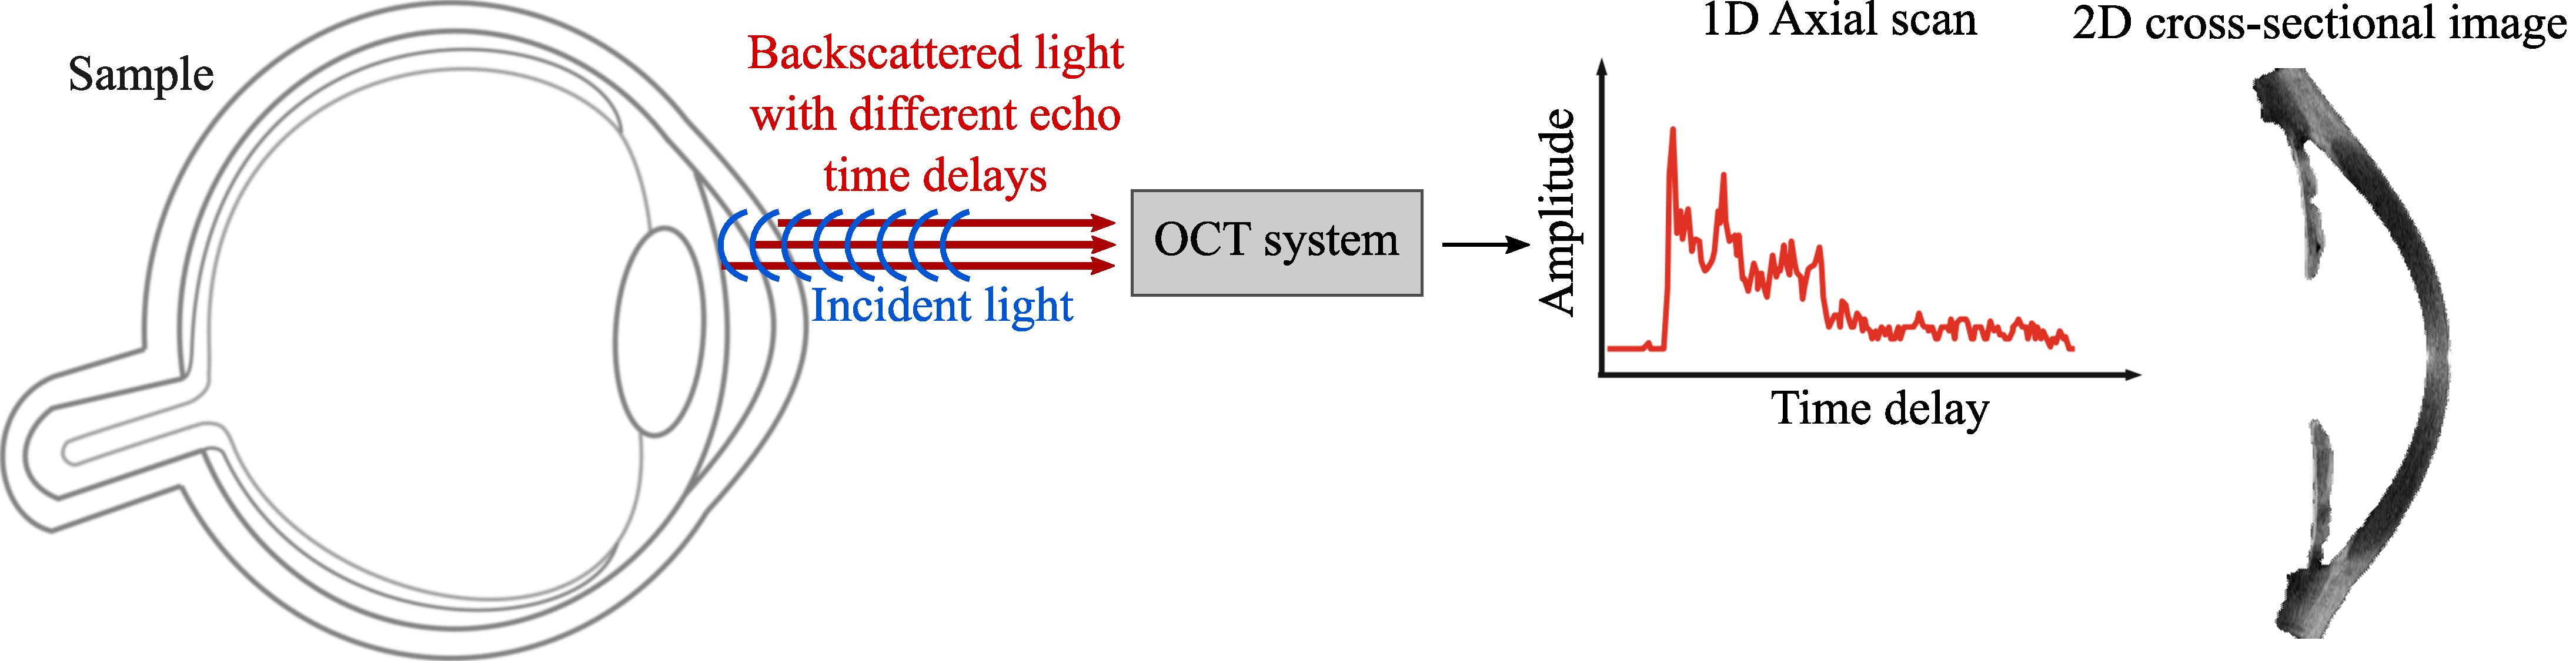
\includegraphics[width=\textwidth]{Figures/Introduction/BasicOCT.pdf}
    \caption{Example of axial scan and cross-section images generated by OCT measuring the magnitude and echo time delay of backscattered light.}
    \label{fig:BasicOCT}
\end{figure}

Providing cross-sectional images \textit{in situ} and in real time without the need to remove and process specimens is an important feature of OCT for the visualization of tissue micro-structure and pathology. This possibility to perform ``optical biopsies''~\cite{Fujimoto1995_Optical} enables operation of OCT in application where histopathology of excised tissue, the gold standard for assessing pathology, is insufficient for various reasons~\cite{Fujimoto2015_Introduction}: (1) biopsy is hazardous or impossible, for example in the eye, arteries or nervous tissues, (2) biopsy is susceptible to sampling errors, given the impossibility to precisely detect the location of the pathology, for example in cancer diagnosis, leading to false negative, (3) real time visualization is required, for instance in guidance of invasive procedures, and (4) structural information is not sufficient and additional functional imaging or measurements like blood flowmetry is necessary.

Several phenomena occur in the interaction of the sample and the incident light. OCT measures only the light that is backscattered, in other words, the light that is scattered in the opposite direction of the incident beam. In that sense, the major limitation of OCT is that light is highly scattered in multiple directions by most tissues reducing the portion of backscattered light, and this attenuation by scattering imposes a limit to imaging depth in OCT to $\sim$2~mm in tissue~\cite{Fujimoto2015_Introduction}. Light sources in the near-infrared range with wavelength between 840--1300~nm are widely used for OCT given the low water absorption and high scattering of tissue~\cite{Schmitt1994_Opticalcoherence}. In general, imaging at $\sim$1300~nm is preferred in most OCT applications because it provides larger imaging penetration compared to shorter wavelengths, although standard for ophthalmology are $\sim$850~nm and $\sim$1~$\mu$m wavelengths~\cite{Fujimoto2015_Introduction}.

OCT has become an important standard for clinical assessment in ophthalmology given that the optical transparency of the eye allows ``easy'' optical access to the retina and to the posterior segment of the eye in general. Actually, first experimental demonstration of OCT imaging in 1991 by Huang \textit{et al}. was performed in human retina and coronary artery \textit{ex vivo}~\cite{Huang1991_Optical}, then following works by Fercher \textit{et al}.~\cite{Fercher1993_Vivo} and Swanson \textit{et al}.~\cite{Swanson1993_Vivo-1} demonstrated retinal images \textit{in vivo}, and since then, ophthalmology has been the specialty with more clinical studies and technical developments in OCT, because it assists in the diagnosis of diseases in early and late stages~\cite{Puliafito1995_Imaging, Chu2007_Clinical, Sathyan2012_Optical}, even before visual symptoms or irreversible consequences occur~\cite{Schuman1995_Quantification}, and it also allows to track progression of diseases and monitor response to therapy~\cite{Carrasco-Zevallos2017_Review, Chang2018_Intelligent, Maltais-Tariant2020_Realtime}.

The most direct application of OCT after ophthalmology is in dermatology given the easy access to skin tissue~\cite{Welzel2001_Optical}. OCT allows readily identification of skin features like sweat ducts, dermal/epidermal junction and collagen-rich structures~\cite{Welzel1997_Optical}, but imaging depth is very limited due to the highly scattering properties of skin tissue~\cite{Carrion2007_Comparative}. Although it is an active application for OCT, for instance in skin cancer diagnosis~\cite{FerrantediRuffano2018_Optical}, medical impact of OCT in dermatology is not as relevant as in ophthalmology given that practical and scientific benefits over standard medical procedures in this field are not clear.

Medical applicability of OCT was extended after the integration of OCT imaging systems with catheters, endoscopes and needles probes that enable operation of OCT in luminal tissue such as gastrointestinal tract~\cite{Jackle2000_Vivo}, vasculature~\cite{Tearney1996_CatheterBased} and airway~\cite{Armstrong2003_Vivo}, as well as in solid organs~\cite{McLaughlin2012_Imaging}. The possibility to image internal body organs \textit{in situ} is particularly important when excision of tissue is not possible or hazardous, for instance in intravascular imaging, which currently is a relevant medical OCT application~\cite{Bouma2017_Intravascular}.

Moving to an experimental description of OCT, the general setup consists in a light source, an optical interferometer such as Michelson or Mach-Zehnder interfermeters, and a light detector~\cite{Huang1991_Optical}, as depicted in Figure~\ref{fig:OCT_ScanningScheme}. In the interferometer, light from the light source is divided into two beams, one is reflected by a mirror, the other by the sample, and both are recombined producing interference that is captured by the detector. The axis in which light propagates is referred as \textit{axial} axis and the orthogonal axes are known as \textit{lateral} or \textit{transverse} axes. Most OCT systems focus the light into a small spot in the sample and acquire the axial scan known as \textit{A-line}, relating the amplitude of the signal versus depth. Then, the position of the focused spot in the transverse plane is changed using two galvanometer mirrors and in each position an A-line is acquired, this is known as \text{raster scan}. Acquisition of A-lines at different positions of the sample along one lateral axis known as \textit{fast scan axis} produces 2D cross-sectional views known as \textit{B-scans}. Acquisition of B-scans at different positions of the sample along the lateral axis that is orthogonal to the fast scan axis, known as \textit{slow scan axis}, provides volumetric images or \textit{tomograms}. Furthermore, the cross-sectional views relating the two lateral axes at a fixed depth are known as \textit{en face}~\cite{Fujimoto2015_Introduction}. See Fig.~\ref{fig:OCT_ScanningScheme} for an illustration of the notation described above. An additional scan used in very particular applications consists in acquiring multiple A-lines in time but at the same location which is known as \textit{C-scan}. 

\begin{figure}
    \centering
    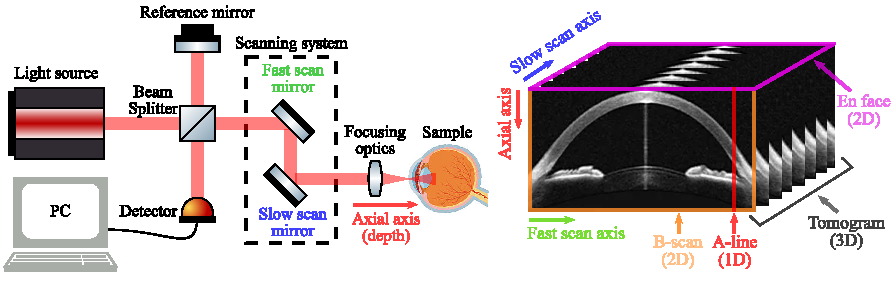
\includegraphics[width=\textwidth]{Figures/Introduction/OCT_ScanningSchemes.pdf}
    \caption[Schematic of a generic OCT setup based on a Michelson interferometer and illustration of common notation.]{Schematic of a generic OCT setup based on a Michelson interferometer and illustration of common notation used for axial axis, transverse axes (fast/slow scan axes), axial scan (A-line) and cross-sectional images (B-scan, \textit{en face}).}
    \label{fig:OCT_ScanningScheme}
\end{figure}

From this general scheme, OCT technology and theory have evolved and to date there is a wide variety of system configurations with particular advantages in terms of imaging speed, sensitivity, imaging depth, among others~\cite{Fujimoto2015_Introduction}. Nonetheless, the use of an optical system to focus the light into the sample and to collect the backscattered light is common to any OCT system and its properties greatly influence the quality of images, most notably, it determines the lateral resolution, i.e. the resolution in the lateral axes, and it may induce optical aberrations that degrade image quality, similarly to any other optical imaging technique~\cite{Ralston2006_Interferometric, Yasuno2006_Noniterative, Adie2012_Computational}.

\section{Aberrations in OCT}

In most OCT systems, light is focused into the sample, so that lateral resolution is defined by the diffraction-limited spot size of the focused light beam~\cite{Fujimoto2015_Introduction}. Optical aberrations, whether from the optical systems or the sample itself, degrade image quality affecting the visualization of fine structures and limiting the axial range where images appear sharp~\cite{Ralston2006_Interferometric,Zawadzki2005_Adaptiveoptics}. To avoid or reduce impact of aberrations, specialized optical systems are used, for instance, telecentric and achromatic systems correct for spherical and chromatic aberrations~\cite{Hu2015_Optical}.

One of the greatest limitations of optical systems is that in-focus images are only obtained for those planes of the sample that are within the \textit{depth of field} (DoF), defined by the numerical aperture (NA) of the system, while beam divergence causes a resolution loss for planes outside the DoF, producing defocused images~\cite{Yasuno2006_Noniterative, Ralston2006_Interferometric}. In the case of OCT, this means that certain planes of the tomogram will be in-focus and appear sharp, but others are out-of-focus and appear blurred. To avoid this, systems with large DoF of $\sim$0.5 -- 2~mm are commonly used so that imaging axial range is limited by signal attenuation in tissue rather than by the effect of defocus. However, this is achieved at the cost of reducing lateral resolution given its inverse relation with DoF, well-known as lateral-resolution--DoF trade-off. For this reason, it is very common that resolution in the transverse plane is lower than resolution in the axial axis, which depends on the central wavelength and spectral bandwidth of the light source and is independent of the NA~\cite{Fujimoto2015_Introduction}.

In addition to system-induced aberrations, the sample can introduce aberrations with a significant impact to reduce image quality, particularly in ophthalmology given that light beam passes through the eye of the subject and imperfections in the cornea and the lens may induce aberrations~\cite{Walsh1984_Objective, Liang1997_Aberrations}.

Because aberrations affect the raw OCT signal, any subsequent post-processing will be influenced by them as well~\cite{Cense2009_Retinal, Park2020_Angiographic}, such is the case of functional imaging techniques like polarization-sensitive OCT (PS-OCT) which is an extension of OCT for measuring the polarimetric properties of the sample~\cite{deBoer1997_Twodimensional}, and OCT angiography (OCT-A) used for vasculature label-free imaging~\cite{Wang2007_Three}.

High-resolution imaging is a very active research field in OCT since it gives access to additional and more detailed information of the sample, which is important in many applications, for example, in cellular imaging as eye photoreceptors~\cite{Zhang2006_Highspeed}. To obtain high-resolution images, aberration can be corrected with hardware-based adaptive optics (AO)~\cite{Zawadzki2005_Adaptiveoptics} or computational aberration correction (CAC)~\cite{Adie2012_Computational}. In AO, additional hardware is used to correct for wavefront distortions \textit{in situ}. It demands complex optics and system design that limits clinical applicability, yet, it is incapable of compensating the lateral-resolution--DoF trade-off given that each depth demands an individual correction but OA applies a global correction~\cite{Pircher2017_Review}.

CAC operates the complex OCT signal using mathematical models based on the propagation of light to compensate aberrations using an appropriate phase filter~\cite{Ralston2006_Interferometric, Yasuno2006_Noniterative, Adie2012_Computational}. CAC addresses lateral-resolution--DoF trade-off but its major limitation is the reduction of signal strength given that acquired signal is weaker in the presence of aberrations, which is an experimental limitation that, in principle, cannot be corrected in post-processing~\cite{Wu2019_Computed}. Currently, operation of CAC is not possible in all OCT systems due to technical limitations that prevent the acquisition of reliable complex-value tomograms~\cite{Shemonski2014_Stability}.

In this work, we present a method for CAC suitable for most common OCT systems to expand its applicability throughout research and clinical applications, making it possible to correct for optical aberration to improve image quality by post-processing in systems where it was not possible due to technical limitations.

\section{Noise in OCT}

Any contribution to the measured signal apart from the backscattered light, that is the interest of OCT, can be considered as \textit{noise}~\cite{Izatt2015_Theory}. In that sense, \textit{speckle} arising in tissue imaging as a consequence of coherent interference of backscattered light with random phases~\cite{Goodman2007_Speckle}, is not noise in rigorous terms, indeed, speckle is important for several functional imaging applications~\cite{Wang2007_Three, Lee2012_Dynamic, Liu2013_Quantitative}, but in practical terms it causes random fluctuations that hinder visual interpretation~\cite{Schmitt1999_Speckle}. Consequently, speckle reduction while preserving visibility of fine structures is an active area of research in OCT~\cite{Cuartas-Velez2018_Volumetric} and in most coherent imaging techniques, such as synthetic aperture radar (SAR)~\cite{Argenti2013_Tutorial}. For this reason, noise reduction in OCT is generally associated with speckle reduction, but there are multiple sources of strictly speaking noise in the OCT signal induced by the system, that have a relevant impact on imaging features such as the \textit{signal-to-noise ration} (SNR), define as the ratio of the signal power and the noise process variance; the sensitivity, defined as the SNR of a perfect reflector placed in the sample arm; and the dynamic range, defined as the range of SNR observable within a signal acquisition or image~\cite{Izatt2015_Theory, deBoer2003_Improved}. SNR is typically given in decibels (dB) through the logarithmic transformation $\text{SNR}_{\text{dB}} = 10\log_{10}\text{SNR}$. Developments in OCT technology had a significant improvement in sensitivity and current imaging systems achieve sensitivities as high as $\sim$100~dB, meaning that minimum detectable reflectivity in the sample is $\sim$1$\times$10$^{-10}$ times the reflectivity of an ideal reference mirror~\cite{Izatt2015_Theory}. In experimental terms, OCT images span dynamic ranges of 40--60~dB although it depends on the tissue and the system.

Most notable sources of noise in the OCT signal are shot, excess and thermal noise~\cite{deBoer2003_Improved}. \textit{Shot} noise originates from the uncertainty of ``counting'' particles of discrete nature such photons and electrons, and it arises in the detection of the OCT signal that involves photon-electron conversion and digitization. \textit{Excess} noise arises from time fluctuations of the incident intensity, mostly due to fluctuation of the emission of the light source. \textit{Thermal} noise stems from random motion of electrons in conductors. In OCT, noise has been addressed mostly experimentally, and at this points it is possible to achieved shot noise limited detection~\cite{deBoer2003_Improved}. For instance, excess noise suppression is achieved using two detectors in a \textit{balanced} detection scheme where non-interfering light ---that contributes the most to excess noise--- is suppressed. Computational approaches for noise reduction have concentrated in speckle suppression, and most shot noise reduction approaches rely on a straightforward average of multiple frame repetitions~\cite{Baumann2019_Signal}.

Reduction of signal strength due to aberrations have a negative impact in SNR and dynamic range because the collected signal is intrinsically lower in the presence of aberrations than in the aberration-free case, and this is not compensated in CAC techniques. An experimental approach to reduce signal strength loss is to use CAC techniques in systems with an astigmatic beam that provides high signal strength throuhout longer depth than a Gaussian beam, so that aberrations are corrected including the astigmatism induced on purpose~\cite{Adie2012_Computational}.


\section{Problem statement}

Post-processing is important in OCT to obtain images with high resolution and contrast as well as additional useful information of the sample, improving and facilitating study, diagnosis and monitory of diseases. Developing techniques to improve image quality in OCT has been the scope of collaborative projects between the Applied Optics Group at Universidad EAFIT and the Wellman Center for Photomedicine at Massachusetts General Hospital and Harvard Medical School. Results include the development of an useful technique for speckle suppresion~\cite{Cuartas-Velez2018_Volumetric}, as well as the derivation of models for robust estimation of the autocorrelation function of intensity OCT signal~\cite{Uribe-Patarroyo2020_Noise} that is the basis of functional imaging modalities such as angiography~\cite{Wang2007_Three} and flowmetry~\cite{Liu2013_Quantitative}. In parallel, experimental setups have been made, including a lab-made accessible full field OCT system~\cite{Cuartas-Velez2019_Labmade} and a linear-in-wavenumber spectrometer for spectral-domain OCT~\cite{Ruiz-Lopera2018_Design}. In addition, a numerical phase correction algorithm was proposed but, given its iterative structure, processing times are and results are limited unpractical~\cite{Cuartas-Velez2017_Formacion}, however, this initial approach for phase stabilization contributed to ideas and notions that led to the current proposal.

Computational aberration correction is a very active field in OCT to improve image quality in application where aberration have a significant impact and to provide high-resolution images~\cite{Adie2012_Computational, Hillmann2016_Aberrationfree, Kumar2017_Invivo}. Development of CAC techniques has been constrained to system configurations that allow a more reliable and robust measurement of the complex-valued tomogram. CAC techniques are based on a common mathematical model, hence requirements for its application are the same, being phase stability the most relevant requirement~\cite{Shemonski2014_Stability}. \textit{Phase stability} is achieved when there is a constant phase relation between measurements at different lateral locations~\cite{Shemonski2014_Stability}, in other words, when there exists a correlation between measurements.

Acquisition of phase stable tomograms is not straightforward in practical terms given that phase is very sensitive to phase noise that affects phase stability~\cite{Shemonski2014_Stability, Vakoc2005_Phaseresolved}, arising from the imaging system and from the sample itself due to axial motion~\cite{Shemonski2014_Stability-1, Shemonski2014_Threedimensional}. In fact, sample motion artifacts include two effects: the first is a phase jump due to Doppler effect~\cite{Chen1997_Optical, White2003_vivo} and the second is the effective shift of the complex information due to sample displacement. Doppler phase noise is the issue most addressed for CAC given that its impact is, in general, more notable than impact of complex-amplitude shift~\cite{Shemonski2014_Stability-1, Shemonski2014_Threedimensional}, although the impact of each effect is relative to features of the imaging system and the amount of motion~\cite{Shemonski2014_Stability}.

Achieving sufficient phase stability for CAC has restricted its usage to custom system configurations with volumetric phase stability, that in some cases is achieved at the cost of increasing system complexity~\cite{Ginner2018_Holographic, Kumar2013_Subaperture, Hillmann2016_Aberrationfree, Sudkamp2018_Simple}. In phase stable systems, operation of CAO is straightforward and for \textit{in vivo} imaging it is sufficient to correct for phase noise due to sample axial motion using numerical corrections based on reference phase signal, generated by adding a highly reflective surface such as a coverslip, or based on the acquired sample signal~\cite{White2003_vivo, Ralston2006_Phase}. Drawback of correction methods based on reference phase signal is that it demands hardware modifications to add a highly reflective surface in addition to the reference mirror.

Numerical phase stabilization methods based on the sample signal assume that there is phase stability at least along one lateral axis, thus correction is only required along the orthogonal lateral axis~\cite{Shemonski2014_Threedimensional}. This assumption is valid for phase stable systems in which phase instabilities in the tomogram arise from sample motion and only affect one lateral axis, commonly the slow scan axis~\cite{Shemonski2014_Threedimensional}. However, there are common OCT configurations that present phase noise induced in the system, for which current numerical phase corrections are hopeless given that there is not any axis with phase stability~\cite{Vakoc2005_Phaseresolved}. Operation of CAO in such phase unstable configurations rely on hardware modifications to avoid system-induced phase noise, restricting its applicability in research and medical application.

Given the current limitation of standard OCT systems to acquire phase stable tomograms, the proposal of this work is \textit{to develop and experimentally test a post-processing method for optical aberration correction in phase unstable tomograms, with no need for hardware modifications or specialized configurations, hence enabling operation of CAC for image quality improvement in system unsuitable for it so far, more specifically, in raster scan wavelength-swept source OCT systems.}

In addition, we also aim to address other important issues in CAC, in regard to the SNR reduction in aberrated tomograms due to signal strength loss, as well as the motion artifacts affecting the complex amplitude, not only the phase.

\newpage
\section{Objectives}
\vspace{\baselineskip}
\subsection{General objective}

To correct optical aberrations in optical coherence tomography with phase unstable systems using post-processing.

\subsection{Specific objectives}

\begin{itemize}
    \item To establish the state-of-art of computational aberration correction in optical coherence tomography.
    \item To identify sources of phase noise and phase correction methods for optical coherence tomography.
    \item To develop a computational method for phase stabilization and aberration correction of tomograms with no intrinsic phase stability.
    \item To test the performance of the method with \textit{ex vivo} and \textit{in vivo} tomograms acquired with typical phase unstable OCT systems.
    \item To identify and analize the possible limitation of the method.
\end{itemize}

\section{Outline of the work}

In this work we present our technique Short Aline-Range Phase-stability adaptive-optics (SHARP) for computational aberration correction in phase unstable systems~\cite{Ruiz-Lopera2020_Computational}, showing successful experimental results using systems with no need for specific hardware that ensure phase stability, in a variety of OCT application ranging from ocular imaging to endoscopic imaging and including \textit{ex vivo} and \textit{in vivo} modalities. SHARP integrates a computational aberration correction technique with numerical phase noise correction to compensate aberrations in phase unstable OCT tomograms, showing particular potential for extending the depth of field to relax the lateral resolution--DoF trade-off.

Additional approaches to address other general drawbacks and limitations of CAC are proposed. Complex noise reduction approaches are presented to countervail the intrinsic reduction of SNR in computational aberration corrected images when compared to experimental aberration-free images. Second, SHARP is extended to admit tomograms affected by complex amplitude shifts due to sample motion for \textit{in vivo} imaging, in addition to Doppler phase term, thus addressing both effects of motion artifacts. Furthermore, an alternative step for correction of spatial-varying aberrations encountered in certain practical scenarios is described. Finally, a strategy to perform computational aberration correction in polarization-sensitive OCT is presented, taking into consideration the particularities of the processing used in this functional imaging technique to properly correct aberrations. Successful computational refocusing of polarimetric properties images of tissue is presented. This is the first integration of computational refocusing in PS-OCT to the best of our knowledge.

There is a particular interest in this work in noise reduction because of its importance not only in CAC but in OCT imaging universally to improve sensitivity and dynamic range. First proposal introduced here for noise reduction is to use a straightforward frequency filter grounded in the context of image deconvolution, that has been used in several imaging modalities, for instance in astronomy, but not in the context of OCT, to the best of our knowledge. In fact, this filter is used for image deconvolution but is not particularly dedicated to noise reduction despite its potential for such purpose.

Second approach is a more sophisticated noise reduction technique that we developed and termed Coherent Tomographic Non-local-means denoising (CTNode). This technique is an adaptation of our previous despeckling technique Tomographic Non-local means despeckling (TNode) where modifications were made in order to address for photon noise in the complex-amplitude tomogram, that is the aim of CTNode, instead of speckle in the intensity tomogram, that is the aim of TNode. Both approaches are based on non-local-means weighted-averaging using statistical properties of its corresponding undesired component, i.e. photon noise or speckle. Experimental results of CTNode are presented in conjunction to SHARP, although applicability of both techniques is independent. CTNode promises to be a more efficient technique than standard approaches based on frames averaging, with potential applications in functional OCT techniques.

\section{Structure of the document}

In this Chapter, a general introduction of OCT was provided to present the problem and the objectives of this work.

In Chapter~\ref{chap:theory}, there is a description of the principle of operation of OCT and the different possible configurations, making emphasis in the level of phase stability that is achieved in each configuration. A mathematical model for the signal of the ``OCT experiment'' is presented from a interferometric perspective and then from a light propagation and image formation perspective. The latter model serves as the basis for the CAC techniques that are then described, followed by a description of phase stability requierment in CAC and phase stabilization techniques, emphasizing in numerical approaches. A simulated tomogram with simple structures generated elsewhere based on the acquisition of the complex OCT signal~\cite{Cuartas-Velez2017_Formacion} is used to illustrate concepts and explanations when required.

Foundation and description of SHARP are given in detail in Chapter~\ref{chap:SHARP}. Results of a proof of concept experiment are presented, in which a cucumber sample presenting remarkable structures was used to acquire tomograms with and without defocus induced intentionally shifting the position of the sample. Furthermore, approaches to address additional important issues in CAC, beside phase stability requirement, are proposed, namely, motion artifacts and spatially-varying aberration correction. Mathematical and conceptual framework of CTNode are also presented in Chapter~\ref{chap:SHARP}, briefly explaining the operation of non-local means algorithm and then deriving its particular operation in CTNode, taking into consideration the origin and statistical description of photon noise in the OCT signal. Results are presented using the simulated noiseless tomogram mentioned previously.

Experimental validation of the methods is presented in Chapter~\ref{chap:results} for a variety of samples, systems and applications, including \textit{ex vivo} and \textit{in vivo} imaging in ophthalmic, endoscopic and dermatologic OCT. Aberration correction with SHARP is demonstrated in anterior segment imaging of swine eye \textit{ex vivo}, endoscopic OCT of swine airway \textit{in vivo}, and skin imaging of human hand dorsal \textit{in vivo} with motion artifacts. Furthermore, it is showed that integration of SHARP and resolution-preserving despeckling technique TNode dramatically improves image quality in comparison to the raw tomograms. Also, noise reduction with CTNode is demonstrated in conjunction with SHARP in anterior segment imaging and independent in human retina imaging \textit{in vivo}, showing a significant noise floor reduction. Additionally, operation of SHARP in PS-OCT based on Stokes processing is demonstrated in the anterior segment of an excised swine eye, showing successful defocus correction in polarimetric parameters of tissue, In each demonstration, a discussion and analysis of the methods and the results are given, highlighting the capabilities and drawbacks.

Finally, conclusions in regard to results and objectives of the work are discussed in Chapter~\ref{chap:conclusions}, as well as possible further steps in the context of noise reduction and computational aberration correction in OCT.
\newpage
\phantomsection
\chapter{Theoretical basis}\label{chap:theory}

There have been several theoretical and technical advances in optical coherence tomography (OCT) in response to the importance that it has gathered in the biomedical optics community~\cite{Fujimoto2015_Introduction}. In this chapter, principle of operation, models for the OCT signal and advances of OCT are explained, including the different configurations that have been developed, starting from the initial approach based on low coherence interferometry in time domain detection~\cite{Huang1991_Optical} that later advanced into spectral domain detection~\cite{Fercher1995_Measurement, Chinn1997_Optical}, and presenting advantages and disadvantages in practical features such as sensitivity~\cite{deBoer2003_Improved}, imaging speed~\cite{Yun2003_Highspeed}, and most importantly here, phase stability~\cite{White2003_vivo} that is discussed in detail. In the first part of this Chapter, Section~\ref{OCT}, the OCT experiment is analyzed from an interferometric perspective in regard to the coherence gating used for axial scan performed in OCT. In second part, Section~\ref{Model}, propagation of light in the sample arm is taken into account to establish a more general model for image formation in OCT, in regard to the confocal gating used for transverse scan. From this model derive the state-of-the-art techniques for computational aberration correction in OCT explained in Section~\ref{CAC}, where also phase stability requirement and approaches to achieved it are discussed.

\section{Optical coherence tomography}\label{OCT}

\textit{Tomography} techniques produce images by sectioning the sample using a penetrating wave~\cite{Guy2005_Introduction}. In medicine, tomography techniques radiate waves into the sample and measure the backscattered waves to produce cross-sectional images of the internal structure of tissues~\cite{Guy2005_Introduction}. For instance, ultrasound employs sound waves and measures the echo time delay and amplitude of the reflected waves~\cite{Szabo2014_Diagnostic}, while light is used in optical coherence tomography. Measuring the echo time delay of light with micrometric resolution using direct electronic detection schemes as in ultrasound is challenging given that light is around six orders of magnitude faster than sound. Therefore, optical ranging measurements demand alternative approaches such as high-speed optical gating~\cite{Duguay1971_Ultrahigh} or low coherence interferometry that is the basis of OCT~\cite{Huang1991_Optical}.

\subsection{Measuring the echo time delay of light}

Using backscattered light to see through biological tissue was proposed by Duguay~\cite{Duguay1971_Light, Duguay1971_Ultrahigh} in 1971 employing a high-speed optical Kerr shutter with a 10~pico-seconds pulsed laser to ``photograph light in flight'' while propagating through a cell of milk and water~\cite{Duguay1971_Ultrahigh}. In subsequent approaches, resolution was improved using nonlinear optical processes to detect the time delay of backscattered light with femto-second resolution, making possible to measure corneal thickness in a rabbit eye \textit{ex vivo} with 15~$\mu m$ resolution~\cite{Fujimoto1986_Femtosecond}. These approaches are unpractical for reasons like the use of intense pulsed lasers and the relatevely low  sensitivity of around $-$70~dB while current OCT systems achieve sensitivities of $-$100~dB, three order of magnitude greater~\cite{Fujimoto2015_Introduction}.

\subsection{Low coherence interferometry}

Potential of low coherence interferometry to measure echo time delay of backscattered light with high resolution and sensitivity was devised in the 80s decade, starting with optical fibers and waveguide devices~\cite{Takada1987_New, Youngquist1987_Optical} and later with biological samples after the first demonstration by Fercher et al. in 1988~\cite{Fercher1988_Eyelength} measuring the axial eye length. Interferometry techniques measures the correlation between optical fields by interfering light that is backscattered by the sample with light that has traveled through a reference path~\cite{Malacara2007_Optical}. In a interferometer, light emitted by the source is splitted into two arms, one is reflected by a reference mirror and the other is reflected by the sample, and then both are recombined to produce interference in a detection plane. Interference only occurs when the optical path length (OPL) difference between the two light beams is within the \textit{coherence length} of the light source $l_c$. This is the optical distance that different waves from the same light source can mismatch and yet maintain a \textit{degree of coherence} or a \textit{correlation}~\cite{Hecht2017_Optics}. % Equivalently, the \textit{coherence time} $t_c$ is the period of time within which the light source emits photons that are correlated, and is related to $l_c$ as $l_c=t_cc$, with $c$ the speed of light.

Coherence of a light source is determined by its emission spectrum: $l_c$ is inversely proportional to emission spectrum bandiwdth. The key insight in high-resolution low coherence reflectometry is the use of light sources with broad spectrum that present short coherence length; \textit{interference signal at a given OPL can be distinguished from interference signals at others OPL with a resolution equal to the coherence length}. This \textit{coherence gating} establishes the principle of axial scan in OCT. For a Gaussian spectrum with central wavelength $\lambda_c$ and full-width at half-maximum $\Delta\lambda$, axial resolution $\delta z$ is

\begin{align}\label{eq:axialRes}
    \delta z = \frac{2\ln 2}{\pi}\frac{\lambda_c^2}{\Delta\lambda}.
\end{align}

Inverse relation between $\delta z$ and $\Delta\lambda$ shows that light source with broad emission spectrum provides high axial resolution. To derive the axial OCT signal, consider the Michelson interferometer depicted in Figure~\ref{fig:OCT_Model}.

\begin{figure}[htb!]
    \centering
    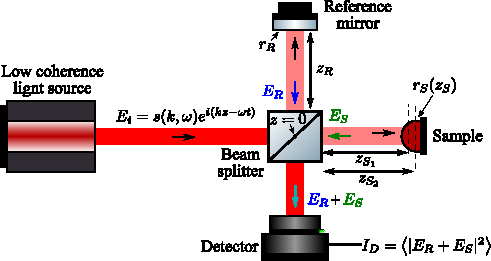
\includegraphics[width=.65\textwidth]{Figures/TheoreticalBasis/OCT_Model.pdf}
    \caption{Schematic of generic Michelson interferometer used in OCT.}
    \label{fig:OCT_Model}
\end{figure}

Interferometry measures the correlation between the electric fields of the light reflected by the sample and the reference mirror~\cite{Malacara2007_Optical}. Consider that the light source emits plane waves with electric field $E_i = s(k,\omega)e^{i(kz-\omega t)}$ at time $t$ and distance $z$ along the propagation axis, being $s(k,\omega)$ the complex amplitude, dependent on the angular frequency $\omega$ and wavenumber $k=2\pi / \lambda$ for wavelength $\lambda$. Assuming free space propagation and a 50/50 beam splitter, the reference beam propagates a distance $z_R$ from the beam splitter to the reference mirror with reflectivity $r_R$ and reflectance $R_R=|r_R|^2$, then reflected light propagates back to the beam splitter and its electric filed can be expressed as $E_R = \dfrac{E_i}{\sqrt{2}} r_R e^{i2kz_R}$.

On the other hand, light on the sample arm propagates a distance $z_S$ from the beam splitter to the sample. In biological tissues, the refractive index changes resulting in different reflectivities, therefore, the sample can be described as a discrete number $N$ of reflectors with reflectivities $r_{S_n}$ and reflectances $R_{S_n}=|r_{S_n}|^2$ located at distances $z_{S_n}$ as
\begin{equation}
    r_S(z_{S_n}) = \sum_{n=1}^N r_{S_n}\delta\left(z_S-z_{S_n}\right).
\end{equation}

\textbf{Coherent gating in OCT allows to reconstruct the function $\mathbf{\sqrt{R_{S_n}(z_{S_n})}}$ to produce images with optical contrast related to changes in the refractive index of the sample.}~\cite{Izatt2015_Theory}

Light backscaterred by the sample propagates back to the beam splitter with electric field $E_S=\dfrac{E_i}{\sqrt{2}}\sum\limits_{n=1}^Nr_{S_n}e^{i2kz_{S_n}}$. Reference and sample electric fields $E_R$ and $E_S$ interfere and a photodetector with responsivity $\rho$ captures the intensity producing a photocurrent $I_D(k, \omega)$ that can be described as~\cite{Izatt2015_Theory}
\begin{align}\label{eq:I_D(k,w)}
    I_D(k, \omega) &= \rho\left<\left|\frac{E_R}{\sqrt{2}} + \frac{E_S}{\sqrt{2}}\right|^2\right> \nonumber\\
    & = \rho\left<\left|\dfrac{E_i}{2} r_R e^{i2kz_R} + \dfrac{E_i}{2}\sum\limits_{n=1}^Nr_{S_n}e^{i2kz_{S_n}}\right|^2\right> \\
    & = \frac{\rho}{4}\left<\left|s(k,\omega) r_R e^{i2kz_R-\omega t} + s(k,\omega)\sum\limits_{n=1}^Nr_{S_n}e^{i2kz_{S_n}-\omega t}\right|^2\right>, \nonumber
\end{align}
assuming $z=0$ at the splitting surface of the beam splitter without loss of generalization, where $\left<\cdot\right>$ is the temporal averaging performed by the photodetector during the integration time of a single measurement, that is long enough to expect that $I_D$ is independent of the temporal component $\omega t$ given the fast temporal oscillation of light imposed by $\omega$. This is consequent with expansion of Eq.~\eqref{eq:I_D(k,w)} using $|E|^2 = E^*E$ that yields the spectral interferogram~\cite{Izatt2015_Theory}
\begin{align}\label{eq:I_D(k)}
I_D(k) &= \frac{\rho}{4}\left[S(k)\left(R_R + \sum_{n=1}^N R_{S_n}\right)\right] ... \nonumber\\
&+ \frac{\rho}{2} \left[S(k)\sum_{n=1}^N\sqrt{R_RR_{S_n}}\cos\left(2k\left[z_R-z_{S_n}\right]\right)\right] ... \\
&+ \frac{\rho}{4}\left[S(k)\sum_{n\neq m}^N\sqrt{R_{S_n}R_{S_m}}\cos\left(2k\left[z_{S_n}-z_{S_m}\right]\right)\right]. \nonumber
\end{align}
where $S(k) = |s(k,\omega)^2|$ is the light source spectrum and $z_R-z_{S_n}$ is the OPL difference.

There are three components in $I_D(k)$ as noted in Eq.~\eqref{eq:I_D(k)}. First one is a \textit{background} component that is independent of propagating distances and it is the largest component given that typically reference mirror reflectivity denominates the sample reflectivity. In general, this is a undesired component that is canceled out using dual balance detection~\cite{Podoleanu2000_Unbalanced}.

Second is a \textit{cross-correlation} component that depends on the spectrum of the light source $S(k)$, the wavenumber $k$ and the OPL difference $z_R-z_{S_n}$. This is the desired component in OCT imaging since it gives access to the sample reflectivity through the term $\sqrt{R_RR_{S_n}}$.

Last term is an \textit{auto-correlation} component that represents the interference between the different sample reflectors, independent of the reference light. This is commonly an artifact component that can be neglected increasing the magnitude of the other two components by increasing the reference mirror reflectivity.

Note that $I_D(k)$ in Eq.~\eqref{eq:I_D(k)} is the interference resulting from a particular wavenumber $k$, but the ultimate aim in OCT is to ``isolate'' the $\sqrt{R_RR_{S_n}}$ term along depth, i.e. versus OPL differences. There are two approaches to retrieve the depth-dependent photoccurent $i_D(z)$, yielding two major OCT configurations: time domain OCT (TDOCT)~\cite{Huang1991_Optical} and Fourier domain OCT (FDOCT)~\cite{Fercher1995_Measurement}.

\subsection{Time domain OCT}

Most straightforward way to obtain the depth-dependent signal is to use a mono-pixel detector to capture the interference while the reference delay $z_R$ is scanned by moving the reference mirror along the axial direction as shown in Figure~\ref{fig:TDOCT_Scheme}. The detector captures the intensity for all $k$ at the same time, thus $i_D(z_R)$ is the integration over all $k$ of $I_D(k)$~\cite{Izatt2015_Theory},
\begin{align}
    i_D(z_R) &= \frac{\rho}{4}S_0\left(R_R+\sum_{n=1}^N R_{S_n}\right)... \nonumber \\
    &+ \frac{\rho}{2}S_0 \sum_{n=1}^N \sqrt{R_RR_{S_n}} e^{-\left(z_R-z_{S_n}\right)^2 \Delta k^2}\cos\left[2k_0\left(z_R-z_{S_n}\right)\right].
\end{align}
where $S_0 = \int\limits_{0}^\infty S(k)dk$ is the spectral total power emitted by the light source, and a normalized Gaussian spectrum $S(k) =\dfrac{1}{\Delta k\sqrt{\pi}}e^{-\big[\frac{(k-k_0)}{\Delta k}\big]^2}$ is assumed, being $k_0$ the central wavenumber and $\Delta k$ the full-width at $1/e$ of the maximum.

\begin{figure}[htb!]
    \centering
    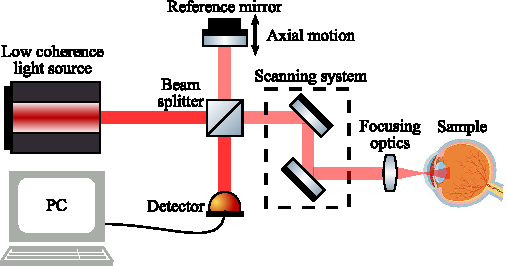
\includegraphics[width=.7\textwidth]{Figures/TheoreticalBasis/TDOCT_Scheme.pdf}
    \caption[Schematic of a generic TDOCT setup based on a Michelson interferometer.]{Schematic of a generic TDOCT setup based on a Michelson interferometer, where axial scan is performed by displacing the reference mirror in the axial axis while recording the interference with a mono-pixel detector.}
    \label{fig:TDOCT_Scheme}
\end{figure}

Time domain A-line $i_D(z_R)$ consists of a background component (DC), proportional to $S_0$, and an interference component that is a summation of Gaussian functions with finite width, having peak-values of $\sqrt{R_RR_{S_n}}$ located at OPL differences $z_R-z_{S_n}$ and modulated by cosines of period $\pi/k_0$, equivalent to $\lambda_0/2$. $\gamma(z_R)=e^{-(z_R-z_{S_n})\Delta k^2}$ is known as the \textit{coherence function} and it causes a ``broaning'' of the interference signal of each reflector and its width is related to the coherence length of the light source that determines the axial resolution, thus $\gamma(z_R)$ is considered as the axial point-spread function (PSF)~\cite{Izatt2015_Theory}. Figure~\ref{fig:Alines} illustrates a TDOCT A-line in Fig.\ref{fig:Alines}(b) for a sample characterized by three reflectors as shown in Fig.\ref{fig:Alines}(a).

\begin{figure}[htb!]
    \centering
    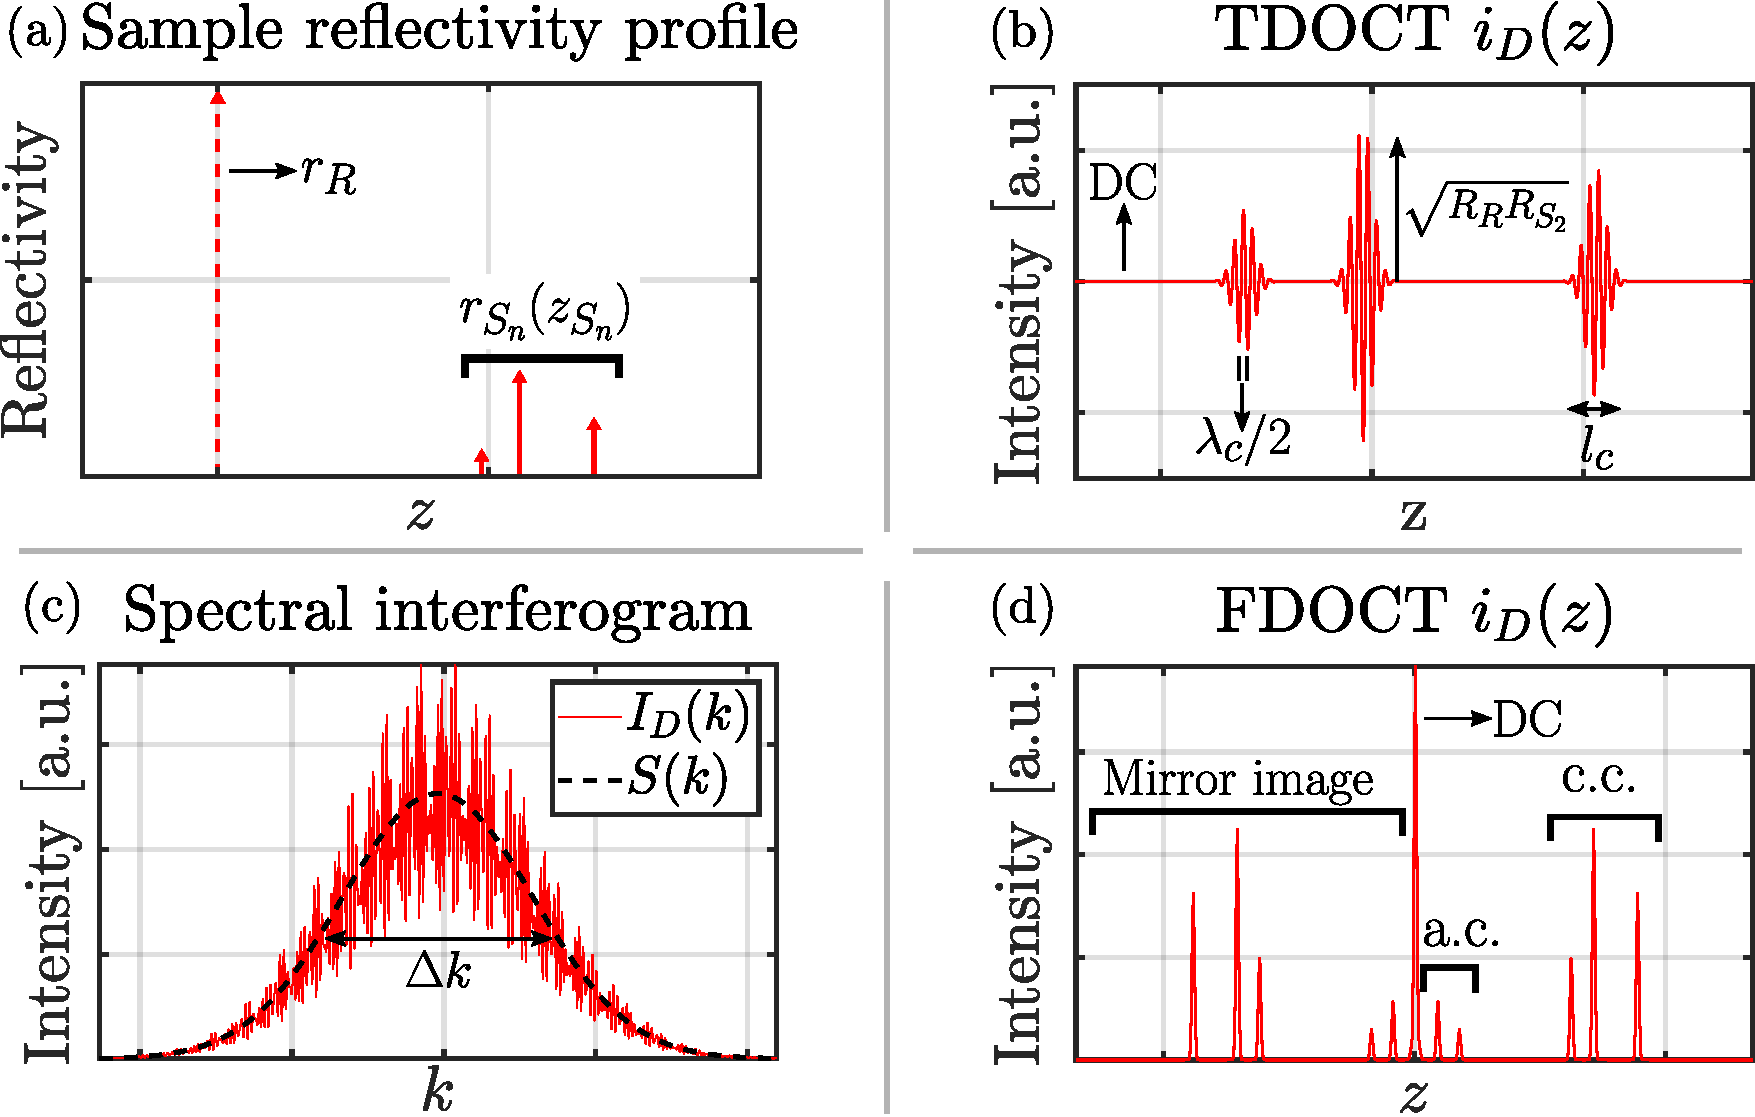
\includegraphics[width=.7\textwidth]{Figures/TheoreticalBasis/Alines.pdf}
    \caption[Illustration of A-lines obtained in OCT.]{Illustration of A-lines obtained in OCT. (a) Axial reflectivity profile for a sample characterized by three reflectors: (b) TDOCT A-line, (c) spectral interferogram and (d) FDOCT A-line obtained as the Fourier transform of (c), indicating the background (DC), cross-correlation (c.c.) and auto-correlation (a.c.) components.}
    \label{fig:Alines}
\end{figure}

Early OCT imaging systems including the first experimental demonstration of OCT in 1991~\cite{Huang1991_Optical} employed a time domain detection. Designation of time domain arises from the fact that the reflectivity axial profile of the sample is acquired while displacing the reference mirror in time. This demands mechanical systems to displace the reference mirror and this limits imaging speed to A-line rates $<\sim$2~kHz~\cite{Izatt2015_Theory}, due to technical restrictions to develop precise fast motion systems with micrometric resolution and millimetric travel range. Furthermore, given that axial scan is acquired while the detector captures the signal at different times, stable systems are required to avoid artifacts during imaging due to changes of the imaging system, for instance, changes of the light source emission. By this reason, achievable sensitivity is limited, and this in addition to low imaging speed establish the major drawbacks of TDOCT~\cite{Leitgeb2003_Performance}.

\subsection{Fourier domain OCT}

Although TDOCT systems served well in early medical OCT development, their relatively slow scan rate and limited sensitivity restricted the potential of OCT and restricted its expansion to many medical applications. An improvement in sensitivity and imaging speed in OCT was possible with the introduction of FDOCT systems where the reference mirror remains fixed~\cite{Choma2003_Sensitivity, Leitgeb2003_Performance, deBoer2003_Improved}. Axial spatial domain and optical frequency domain are conjugates with the wavenumber and the OPL difference being Fourier transform duals. This concept led to development of Fourier domain acquisition where photocurrent $I_D(k)$ in Eq.~\eqref{eq:I_D(k)} is captured directly in the $k$ space and a subsequent Fourier transform $\text{FT}_k\left\{\cdot\right\}$ of the signal  along variable $k$ yields the depth-dependent photocurrent $i_D(z)$, with not need to displace the reference mirror~\cite{Fercher1995_Measurement}.

Using the Fourier transform property $\text{FT}_k\left\{\cos(kz_0)\right\} = \frac{1}{2}\left[\delta\left(z+z_0\right) + \delta\left(z-z_0\right)\right]$, the convolution theorem $\text{FT}_k\left\{g\left(k\right)f\left(k\right)\right\} = \text{FT}_k\left\{g\left(k\right)\right\} \ast \text{FT}_k\left\{f\left(k\right)\right\}$, and the shifting property of delta functions $f(z)*\delta\left(z-z_0\right) = f(z_0)$, it is possible to obtain the FDOCT A-line $i_D(z) = \text{FT}_k\left\{I_D(k)\right\}$ from Eq.~\ref{eq:I_D(k)} as~\cite{Izatt2015_Theory}
\begin{align}\label{eq:i_D(z)}
    i_D(z) &= \frac{\rho}{8}\gamma\left(z\right)\left[R_R + \sum_{n=1}^NR_{S_n}\right] ... \nonumber\\
    &+ \frac{\rho}{4}\sum_{n=1}^N \sqrt{R_RR_{S_n}} \left[\gamma\left(2\left[z_R-z_{S_n}\right]\right) + \gamma\left(-2\left[z_R-z_{S_n}\right]\right)\right]...\\
    &+ \frac{\rho}{8}\sum_{n\neq m=1}^N \sqrt{R_{S_n}R_{S_m}} \left[\gamma\left(2\left[z_{S_n}-z_{S_m}\right]\right) + \gamma\left(-2\left[z_{S_n}-z_{S_m}\right]\right)\right], \nonumber
\end{align}
where again $\gamma\left(z\right)=\text{FT}_k\left\{S(k)\right\}$ is the coherence function of the source, that assuming a Gaussian emission spectrum is given by
\begin{align} \label{eq:SGamma}
    S(k) =\frac{1}{\Delta k\sqrt{\pi}}e^{-\big[\frac{(k-k_0)}{\Delta k}\big]^2} \xleftrightarrow{\hspace{8 pt}\text{FT}\hspace{8 pt}} \gamma(z) = e^{^{-z^2\Delta k^2}}.
\end{align}

Eq.~\eqref{eq:i_D(z)} contains three components as Eq.~\eqref{eq:I_D(k)}; background, cross-correlation and auto-correlation components. Figure~\ref{fig:Alines} shows an example of a Fourier domain A-line in Fig.~\ref{fig:Alines}(d) for a sample with three reflectors as shown in Fig.~\ref{fig:Alines}(a) and its corresponding interferogram in $k$ space in Fig.~\ref{fig:Alines}(c). Cross-correlation component provides access to the signal of interest in OCT $\sqrt{R_RR_{S_n}}$ by each reflector appearing at positions $\pm2(z_R-z_{S_n})$ and being ``broadened'' by the coherence function similarly to the case of the TDOCT A-line. The apparent position of the reflectors $\pm2(z_R-z_{S_n})$ have a factor of 2 since the interferometer measures the round-trip distance.

There is a ``mirror image'' produced by the fact that $I_D(k)$ is real, hence its Fourier transform is Hermitian symmetric, that is, the positive values are the complex conjugate of the negative values, and this is represented in the double sign of $\pm2(z_R-z_{S_n})$. This does not have an important influence if the sample is positioned entirely in one side of the zero OPL, such that it is possible to extract only one half of the Fourier spectrum to avoid the mirror image.

Background component appears as a large component centered at the zero OPL. In general, it can be easily omitted from the signal since the reflectors of the sample are positioned beyond the zero OPL such that cross-correlation terms do not overlap with the background component. However, additional to the main lobe, side lobes may appear and cause significant artifacts overlapping with the cross-correlation terms, therefore, background is typically removed by recording the spectrum of the source blocking the light from the sample arm and then subtracting this background spectrum to every measurement.

Autocorrelation component appears near the zero OPL if the position of the reference mirror is such that $(z_{S_n}-z_{S_m}) << (z_R-z_{S_n})$, and this way it is possible to omit this artifact, but a more direct solution is to adjust the reference reflectivity to ensure that amplitude of cross-correlation terms are much higher than amplitude of auto-correlation terms.

Note that the OCT signal $i_D(z)$ is given as a function of depth for a specific transverse point with coordinates $(x,y)$ of the sample. In raster scan systems, the beam is scanned in the sample plane using galvanometer scan mirror that deflects the light beam changing its position in the sample, and in each location $(x,y)$ an A-line is acquired. Given that the interest so far is the axial scan, dependence on coordinates $(x,y)$ has been omitted for simplicity.
 
Sensitivity improvement in FDOCT with respect to TDOCT arises from the fact that interference for all depths are captured simultaneously, considering that the signal is acquired in $k$ space and it is known that each value in frequency domain contributes to all values in spatial domain~\cite{deBoer2003_Improved}. In FDOCT, there are two approaches to measure the spectral interferogram. Most intuitive way is to use a digital spectrometer as detector as shown in Figure~\ref{fig:SDOCT_Scheme}, which provides the intensity signal as a function of wavenumber $I_D(k)$ in a single measurement, and it is known as spectral domain OCT (SDOCT)~\cite{Fercher1995_Measurement}. Digital spectrometers are composed of a linear camera and an optical system that separates the spectral components of input light in such way that each pixel of the detector captures the intensity of a portion of the spectrum~\cite{Neumann2014_Fundamentals}. Imaging speed in SDOCT is limited by acquisition rate of the linear camera and typical A-line rates are between 2 -- 50~kHz~\cite{Fujimoto2015_Introduction}.

\begin{figure}
    \centering
    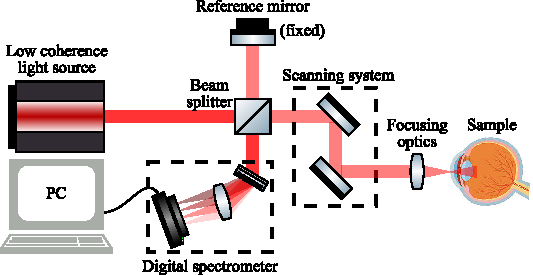
\includegraphics[width=.75\textwidth]{Figures/TheoreticalBasis/SDOCT_Scheme.pdf}
    \caption[Schematic of a generic SDOCT setup based on a Michelson interferometer.]{Schematic of a generic SDOCT setup based on a Michelson interferometer, where axial scan is obtained by computing the Fourier transform of the spectral interferogram acquired with a digital spectrometer.}
    \label{fig:SDOCT_Scheme}
\end{figure}

The second approach in FDOCT is to use a tunable light source with a narrow spectrum and to acquire the interference signal $I_D(k)$ with a single-element photodetector while the central emission wavenumber $k$ of the light source is swept among a broad spectrum, and it is known as wavelength-swept source OCT (SSOCT)~\cite{Chinn1997_Optical, Yun2003_Highspeed}. It is also referred as optical frequency domain imaging (OFDI)~\cite{Bouma2015_Optical} instead of low coherence interferometry given that, in rigorous terms, instantaneous emission of the tunable light source is considered coherent. OFDI achieves the highest imaging speed in OCT, presenting A-line rates up to 200~kHz~\cite{Okabe2012_200}, or even more with specialized instrumentation~\cite{Oh2010_400}, and it is limited by the sweeping rate of the light source. Here OFDI and SSOCT are used indistintively although in general OFDI is used to refer to the imaging technique and SSOCT is used to refer to the OCT systems itself. A more detailed description of SSOCT systems is provided below, because this is the one of interest for this work.

\subsection{Optical frequency domain imaging}

Operation of OFDI is grounded on the fact that OPL and wavenumber are conjugate variables. In low coherence interferometry, interference is acquired illuminating the sample with light spanning several wavenumbers while OPL is scanned. In the alternative scenario, interference corresponding to all OPLs is acquired  at the same time, while illuminating the sample with light spanning a single wavenumber that is scanned, and this is the principle of operation of OFDI~\cite{Yun2003_Highspeed}. Then, a Fourier transform of the signal in spectral domain yields the depth-dependent signal.

Detection scheme in OFDI employs a single-element detector, allowing higher A-line rates than in SDOCT systems that are limited by the acquisition rate of the linear camera, which is composed of multiple pixels. Increasing imaging speed reduces motion artifacts when imaging \textit{in vivo} and allows larger scans in limited time. Tunable light sources are available in the 1--1.3~$\mu$m wavelength range, where cameras technology is not well established, hence SSOCT systems are used commonly in the 1--1.3~$\mu$m range that serves for multiple medical applications and SDOCT in the complementary 0.85--1~$\mu$m range used mainly in ophthalmology~\cite{Fujimoto2015_Introduction}.

The most relevant specifications of tunable light sources in SSOCT are repetition rate, instantaneous linewidth $\delta\lambda$, tunable range $\Delta\lambda$ and tuning curve $k_i(t)$~\cite{Yun2015_Wavelength}. Axial resolution is determined by central wavelength of emission $\lambda_c$ and tunable range $\Delta\lambda$ equally to Eq.~\ref{eq:axialRes}, $\delta_z = \frac{2\ln 2}{\pi}\frac{\lambda_c^2}{\Delta\lambda}$, thus it is independent of instantaneous linewidth. Instead, the depth range $\Delta z$ observed within a single A-line is determined by the instantaneous linewidth as
\begin{align}
\Delta z = \dfrac{\lambda_c^2}{4\delta\lambda}
\end{align}
and is independent of tunable range. Note that central wavelength mediate in both parameters. As a numerical example, a tunable light source with instantaneous linewidth $\delta\lambda=0.1$~nm and tunable range $\Delta\lambda=125$~nm centered at $\lambda_c=1.3~\mu$m provides $6~\mu$m axial resolution along $4.2$~mm depth range. The same light source but with central wavelength $\lambda_c=860$~nm provides $2.7~\mu$m axial resolution over $2.15$~mm.

Tunable curve $k_i(t)$ determines the instantaneous wavenumber as a function of time $t$. Ideally, this is a linear curve $k_i(t) = k_0 + k_st$ where $k_0$ is the initial wavenumber and $k_s$ is the wavenumber step between consecutive instantaneous wavenumbers~\cite{Dorrer2000_Spectral}. In practice, $k_i(t)$ is a non-linear function of time and thus linearization is required, typically performed on post-processing prior to computing the Fourier transform of the spectral interferogram, otherwise, artifacts appear degrading axial resolution~\cite{Dorrer2000_Spectral}.

Development of SSOCT systems have inherited technology from optical communications in the near infrared spectrum that employs similar optical components such as tunable laser sources, optical fiber and detectors~\cite{Yariv2007_Photonics}. In that sense, there are multiple types of tunable light sources relying on different principles of operations, but currently the development of fast, stable, linear, low-cost tunable light sources is a very active area of research~\cite{YasinAlibhai2018_Swept}.

Lasers are optical oscillators comprising a gain medium that is pumped optically or electrically to amplify light by stimulated emission, and an optical cavity that gives coherent optical feedback for laser oscillations~\cite{Saleh1991_Fundamentals}. Semiconductor optical amplifier (SOA) is a gain medium widely used for tunable lasers because they offer a high gain in a broad bandwidth, a rapidly response time, in the picosecond scale, and a wide range of gain center wavelengths depending on the semiconductor materials~\cite{Yun2015_Wavelength}. One way to construct tunable lasers is to incorporate in the basic laser instrumentation an internal or external scanning filter to select the central wavelength of the instantaneous emission. One of the first approaches developed for OCT applications was tunable laser based on scanning filter using a polygonal mirror and to date this is widespread in research and medical systems~\cite{Yun2003_Highspeed}. Polygon-based tunable lasers offer high sweep rate in a wide tuning range with narrow linewidth, ideal features for OCT imaging.

In polygon-based lasers, the optical cavity includes a diffraction grating, a telescope and a rotating polygonal mirror with tens of facets~\cite{Yun2003_Highspeed}. Light emitted by a SOA within a broad spectrum is reflected by the diffraction grating in such way that there is an angular separation of spectral components. Light is relayed to the polygonal mirror through the telescope, and only the spectral component incident perpendicular to the mirror surface is reflected back to the grating and then to the SOA, proving a coherent light feedback. Rotation of the polygonal mirror changes surface angle and therefore the instantaneous spectral component that has perpendicular incidence also changes~\cite{Yun2003_Highspeed}. Drawbacks of this scanning filter approach is that polygonal mirror is a relatively bulky and moving part.

Figure~\ref{fig:SSOCT_Scheme} illustrates an optic fiber-based SSOCT system using a polygon-based tunable laser. Light from the tunable laser is delivered to an optic fiber beam splitter that divides the light into the sample and reference arms, then, reflected light from both produce interference that is detected by a photodetector and digitized. In this scheme, balanced detection is illustrated using two detectors to subtract the background signal and thus suppressing excess noise\cite{Podoleanu2000_Unbalanced}. Moreover, SSOCT systems require a trigger signal to synchronize detector acquisition with rotation of the polygonal mirror~\cite{Vakoc2005_Phaseresolved}. In the system of Fig.~\ref{fig:SSOCT_Scheme}, the trigger signal is generated by a narrowband fiber Bragg grating (FBG) that reflects light of a specific wavelength, thus when the laser source emits this wavelength, the FBG reflects light generating a pulse that indicates the beginning of interferogram acquisition, performed using N analog-to-digital conversions (ADC) following a sample clock~\cite{Vakoc2005_Phaseresolved}.

\begin{figure}[htb!]
    \centering
    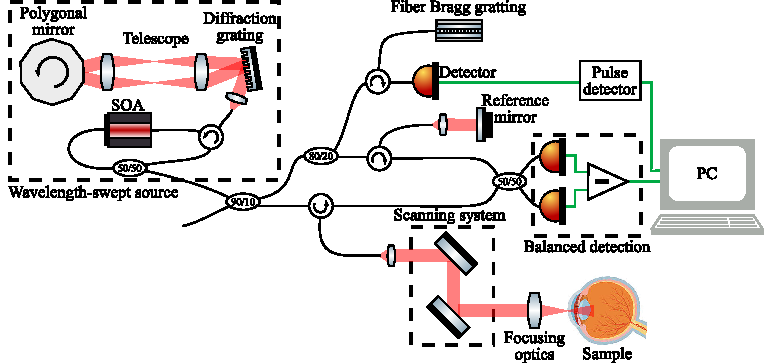
\includegraphics[width=\textwidth]{Figures/TheoreticalBasis/SSOCT_Scheme.pdf}
    \caption[Schematic of a fiber-based SSOCT setup.]{Schematic of a fiber-based SSOCT setup where the wavelength-swept source changes its instantaneous central wavelength in time due to the rotation of the polygonal mirror. A trigger signal to start the acquisition of the spectral interferogram is produced by the fiber Bragg grating that is designed to reflect a single wavelength, indicating the start of a sweep cycle of the light sorce.}
    \label{fig:SSOCT_Scheme}
\end{figure}

Compact tunable lasers have been possible with vertical cavity surface emitting lasers (VCSEL) in conjunction with a micro-electro-mechanical mirror system (MEMS) used to vary the cavity length of the VCSEL, thereby tuning the output wavelength~\cite{Vail1995_Tunable}. MEMS-VCSEL sources however have a limited tuning range and broad instantaneous linewidth although they are in current development to provide a powerful alternative to polygonal-based sources~\cite{Jayaraman2011_OCT}. In addition, current research focuses in developing akinetic tunable lasers to provide more robust and reliable light sources with the same or even better features of polygon-based sources~\cite{Lee2018_Akinetic}.

\subsection{Phase stability in OCT configurations}\label{sec:OCTConfigPhaseStab}

Being an interferometric technique, OCT provides information of the \textit{complex amplitude} of the light backscattered by the sample, and this includes phase and amplitude information. This is an important feature of OCT because the complex amplitude provides more information than the amplitude (or intensity) alone, enabling operation of phase-resolved functional techniques and phase-dependent post-processing~\cite{Park2020_Angiographic, Vakoc2005_Phaseresolved, White2003_vivo}.

In OCT, there are several undesired contributions to the phase that are considered as \textit{phase noise}, arising from the system or from the sample~\cite{Vakoc2005_Phaseresolved, Shemonski2014_Stability}, making development of phase-resolved OCT technology challenging. The ability of a system to provide repeatable phase measurements is known as \textit{phase stability} and it exists when there is a constant phase relation between measurements, that is, when the phase difference between entirely correlated measurements is zero~\cite{Shemonski2014_Stability}. In phase sensitive techniques like flowmetry, phase difference between successive measurements is directly related to the flow velocity, and phase stability is crucial because phase noise causing phase fluctuations adds spurious contribution to the calculation of the phase difference inducing errors in the velocity estimation~\cite{White2003_vivo}.

Phase stability is greatly influenced by the configuration used for axial and transverse scan, and it is possible to obtain 1D (along one axis), 2D (along two axis), or 3D (volumetric) phase stability. In SDOCT, the parallel acquisition of the entire spectral interferogram within a single measurement ensures phase stability during acquisition of every A-line, thus axial axis is phase stable. In addition, the high repeatability of spectrometers ensure phase stability along successive A-lines measured at different times while scanning the beam in the sample, hence in principle SDOCT provides volumetric phase stability. However, there are two additional sources of phase noise in OCT, one induced by sample motion that is detailed in Section~\ref{sec:phaseStab}, and second is induced in the galvanometer scanning system, due to separation of the pivot position of each galvanometer mirror and the back focal plane of the scan lens that adds a phase offset depending on the instantaneous angle of the mirror~\cite{Shemonski2014_Stability}. Although there is a physical limitation in positioning the pivot point of both galvanometers mirrors at the back focal length of the scan lens, precise alignment of one mirror would ensure phase stability along its corresponding lateral scan axis, resulting in 2D phase stability~\cite{Vakoc2009_Statistical}.

In SSOCT systems, achieving phase stability have been more challenging than in SDOCT because each component of the spectral interferogram is acquired sequentially in time and not in parallel like in a spectrometer. In principle, this is not a limitation if experimental conditions of the system during A-line acquisition do not change, but there is a particular issue in regard to the trigger signal that have a detriment effect in phase stability. SSOCT systems require a trigger signal to synchronize A-line acquisition with wavelength sweep of the light source~\cite{Vakoc2005_Phaseresolved}, for instance using a Fiber Bragg grating like in Fig.~\ref{fig:SSOCT_Scheme}. However, the fast sweeping cycle of the light source demand precise electronics to obtain a perfect synchronization, but in practice this is not the situation and there is a time delay or \textit{jitter} in the sample clock for acquisition with respect to the trigger signal. as a consequence, acquisition starts arbitrarily within the sweep cycle of the light source~\cite{Vakoc2005_Phaseresolved}.

A jitter in synchronization causes a shift $\delta k$ in the acquired spectral interferogram, thus the measured signal is $\tilde{I}_D(k) = I_D(k-\delta k)$. Depth-dependent signal obtained as $i_D(z)= \text{FT}_k\{\tilde{I}_D(k)\}$ results in~\cite{Hong2012_Highpenetration}
\begin{align} \label{eq:phaseJitter}
    \tilde{i}_D(z) &= \text{FT}_k\{I_D(k-\delta k)\} \nonumber \\
    &=  \text{FT}_k\{I_D(k)\} e^{-i2\pi z\delta k} \nonumber \\
    &=  i_D(z) e^{-i2\pi z\delta k}
\end{align}
being $i_D(z)=\text{FT}_k\{I_D(k)\}$ the unmodified depth-dependent A-line. Note that effect of spectral shift only impacts the phase of the A-line by the factor $e^{-i2\pi z\delta k}$ that represents a phase ramp with slope $-2\pi\delta k$, known as \textit{phase jitter} noise, but the amplitude $|\tilde{i}_D(z)|=|i_D(z)|$ remains unchanged, thereby traditional structural OCT image based on the intensity $|\tilde{i}_D(z)|^2=|i_D(z)|^2$ is not affected. The random behavior of jitter in synchronization causes that the spectral shift $\delta k$ varies randomly between spectral interferograms, and this dramatically impacts phase stability in raster scan systems because A-lines are captured sequentially in time while displacing the beam in the sample plane, inducing spatially-varying phase-jitter noise.

An approach to avoid phase-jitter is the use of $k$-clocks that produce a sample clock linear in $k$ using a Mach-Zehnder interferometer~\cite{Johnson_Multispeed}. In standard systems, signal acquisition is performed linearly in time with $N$ ADC following an internal electronic sample clock. With a $k$--clock, ADC are performed linearly in $k$ with certainty. Therefore, the use of a $k$--clock avoids phase-jitter because the uncertainty in trigger signal is solved, at the same time that acquired signal is linear in $k$ eliminating the need of signal linearization in post-processing. Although there are $k$-clocked SSOCT systems available~\cite{Kumar2017_Invivo}, they are not widespread because the need of additional hardware, thus phase-jitter is a very common issue affecting standard research and medical OCT systems~\cite{Bouma2015_Optical}. Additionally, even using a $k$-clock, SSOCT systems are sensitive to galvanometer and sample motion phase noise, affecting its phase stability~\cite{Shemonski2014_Stability-1}.

In the previous descriptions, it is possible to note that phase stability is very limited in raster scan systems, whether SDOCT or SSOCT, because transverse scan is performed in time. Parallel acquisition of A-lines for different transverse location can be achieved with extended-field systems where light is projected onto the sample in an extended area. In line-field SDOCT (LF-SDOCT), the sample is illuminated with a line-shaped beam produced by a cylindrical lens and the linear detector in the digital spectrometer is replaced by a two-dimensional detector; one dimension correspond to the $k$ space and the orthogonal dimension corresponds to the transverse fast scan axis~\cite{Nakamura2007_Highspeed, Ginner2017_Noniterative}. Hence, a single acquisition of the detector provides a B-scan view, and a single galvanometer is required to scan the beam along the slow scan axis providing three-dimensional images. Parallel acquisition along fast scan axis ensures phase stability \textit{in vivo} in this axis as long as acquisition rate is relatively fast compared to the velocity of the sample motion, nonetheless, slow scan axis typically remains phase unstable~\cite{Ginner2017_Noniterative}.

TDOCT and SSOCT systems allow full field (FF) acquisition~\cite{Dubois2002_Highresolution, Hillmann2016_Aberrationfree} where the sample is illuminated with an extended collimated beam, the single-element detector is replaced by a two-dimensional detector and additional optical lenses are used to image the sample plane on the detector plane, hence a single axial scan provides an entire tomogram with volumetric phase stability, even \textit{in vivo} if acquisition rate is relatively fast compared to the velocity of the sample motion. Figure~\ref{fig:LF_FFOCT_Scheme} illustrates simple schematics of LF-SDOCT and FF-SSOCT systems.

\begin{figure}
    \centering
    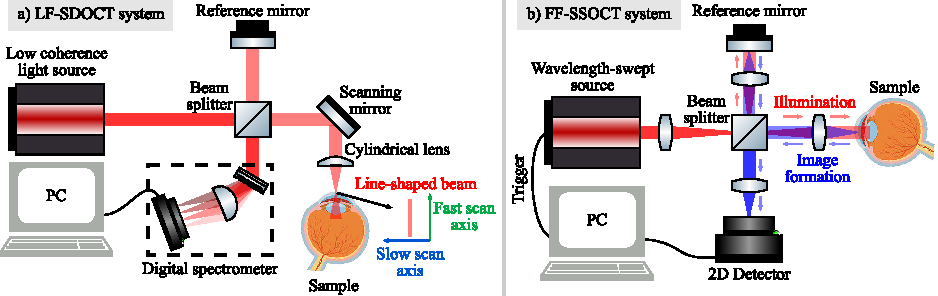
\includegraphics[width=\textwidth]{Figures/TheoreticalBasis/LF_FFOCT_Scheme.pdf}
    \caption[Schematic of generic LF-SDOCT and FF-OSCT setups.]{Schematic of generic (a) LF-SDOCT setup for acquisition of a B-scan in a single detector shot and (b) FF-SSOCT setup for acquisition of a tomogram in a single cycle of the wavelength-swept source. Red path illustrates the illumination beam and blue path the image formation on detector plane for a point.}
    \label{fig:LF_FFOCT_Scheme}
\end{figure}

Extended-field OCT systems are custom configurations used in particular scenarios, like in the CAC research area because they offer sufficient phase stability~\cite{Kumar2013_Subaperture, Hillmann2016_Aberrationfree}, but they are not widespread given that they have a more complex optical design including 2D detectors that are not well developed in terms of speed and sensitivity in the near-infrared range, but more importantly, they are more prone to multiple scattering~\cite{Karamata2005_Multiple}. Scattered light in tissue can be divided into two components: single scattering and multiple scattering (MS), the former is the backscattered signal of interest in OCT and the latter is an undesired component arising from light that is scattered multiple times following random paths that reaches the detector, but it does not contribute direct information to the OCT signal due to its random properties~\cite{Karamata2005_Multiple-1}. Raster scan systems have an intrinsic rejection to MS given because of confocal gating, that is, the focused beam scans a small region of the sample in a limited field of view (FoV), contrary to extended detection that is more prone to collect MS photons given that the FoV during each measurement is larger~\cite{Karamata2005_Multiple}.

There is not a general way to evaluate phase stability. Typically, assessment is performed by visually inspecting phase images, or more specifically images or histograms of phase differences between adjacent A-lines~\cite{Minneman2015_MEMS}. Other possible quantitative approach is to image a coverslip or a reflective surface that is expected to have a constant phase therefore the estimation of phase differences between consecutive A-lines yields an estimation of phase stability~\cite{Minneman2015_MEMS}. One possible configuration to image the coverslip is to acquired A-lines while sweeping the beam with the galvanometer system, thus acquiring a B-scan, or simply by acquiring multiple A-lines at the same position with a static beam what is known as a C-scan. Typical, the standard deviation (STD) of phase differences is provided and used as a quantitative reference of phase stability. For instance, a phase stability of 0.32–5.2~mrad STD has been reported for SD-OCT~\cite{White2003_vivo, Joo2005_Spectraldomain}, whereas 32~mrad STD has been reported for SS-OCT systems using a polygon mirror-based laser~\cite{Manapuram2009_Phasesensitive} using phase stabilization methods, showing that this configuration is indeed more prone to phase instabilities than SD-OCT, but a higher phase stability of 1.5~mrad STD using Akinetic swept laser has been obtained with SS-OCT systems~\cite{Choi2013_Phasesensitive}.

\section{Modelling the acquisition of the complex OCT signal}\label{Model}

In previous section, OCT experiment was described and analyzed from an interference perspective to derive the acquisition of axial scan that provides the depth-dependent signal by means of optical interferometry, however, this signal corresponds to the complex field of backscattered light by the sample but the ultimate aim is to obtain the \textit{scattering potential} of the sample denoted as $\eta$ that gives information of sample structure~\cite{Ralston2006_Inverse}. In other words, in OCT the optical beam probe is used to measure $\eta$ indirectly; the acquired signal contains the sample scattering information as well as the effect of the optical system. In the ideal situation, the effect of the optical system is not significant and the measured signal is directly related to $\eta$. This is the case of systems with aberration-free optical beams where imaging is diffraction-limited inside the depth-of-field and the theoretical lateral resolution is achievable, but in the presence of aberrations or outside the depth of field of the beam, the optical field is distorted and effective lateral resolution is reduced~\cite{Ralston2006_Inverse}.

Scattering theory can be used to derive a model of the imaging formation process that relates the measured signal with the sample structure, known as \textit{forward model}~\cite{Ralston2006_Inverse, Ralston2006_NonParaxial}. Inversion of the forward model results in the \textit{inverse scattering model} that allows to recover an approximate sample structure from the backscattering signal~\cite{Ralston2006_Interferometric}. Solutions to the inverse scattering model brought the development of computational techniques for aberration correction of OCT tomograms~\cite{Ralston2006_Interferometric, Yasuno2006_Noniterative, Adie2012_Computational}. In this section, the forward model is presented and subsequent section surveys solutions to the inverse scattering model to correct aberrations in post-processing.

\subsection{Confocal gating for lateral scan in OCT}

In raster scan systems, the transverse scan is performed using confocal gating resulting from the distribution of the focused beam as shown in Figure~\ref{fig:FocusingLens}. When light is focused on the sample plane, the illuminated cross-sectional area defines the lateral resolution and it can be given in terms of the input beam diameter~\cite{Yasuno2006_Noniterative}. Typically, at the back focal length of the optical system, the probe beam with central wavelength $\lambda_c$ is a Gaussian beam with a $1/e^2$--diameter $D$, and after the optical system, light is focused at the front focal length $f$ in a spot with a $1/e^2$--radius $w_0$ that defines the diffraction-limited lateral resolution $\delta x$~\cite{Fujimoto2015_Introduction}
\begin{align}
    \delta x = 2w_0 = \frac{4\lambda_c}{\pi} \frac{f}{D},
\end{align}
where $\dfrac{D}{2f} = \text{NA}$ is the numerical aperture of the optical system. The inverse relation of NA and $\delta x$ means that high NA systems produce small focused spots and therefore provide fine transverse resolution.

\begin{figure}[htb!]
    \centering
    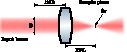
\includegraphics[width=.6\textwidth]{Figures/TheoreticalBasis/FocusingLens.pdf}
    \caption[Schematic of focusing optics in OCT.]{Schematic of focusing optics in OCT. Input collimated beam of diameter $D$ at the back focal length (BFL) is focused into focal point of diameter $\delta x$ at the front focal length (FFL).}
    \label{fig:FocusingLens}
\end{figure}

Due to convergence and divergence of the optical beam, the $1/e^2$--radius $w(z)$  of the focusing beam varies with depth $z$, and setting $z=0$ at the front focal plane, $w(z)$ ca be expressed as~\cite{Ralston2005_Deconvolution}
\begin{equation}\label{eq:beamWaist}
    w(z) = w_0 \sqrt{1 + \left(\frac{z\lambda_c}{\pi w_0^2n}\right)^2}
\end{equation}
where $n$ is the refractive index of the propagating medium.

Eq.~\ref{eq:beamWaist} shows that diffraction-limited resolution is only possible at the focal plane ($z=0$) and is degraded for other planes. However, for distances $z$ relatively close to the focal plane, change of spot size is relatively small. The confocal parameter $b$ is defined as the distance within which the spot size is smaller than $\sqrt{2}\delta x$ and thus resolution can be considered as nearly constant, and it is given by~\cite{Ralston2005_Deconvolution}
\begin{equation}
    b = 2z_R = \frac{\pi\delta x^2}{\lambda}
\end{equation}
where $z_R$ is known as the Rayleigh range. Confocal parameter defines the region where defocus is negligible and is also referred to as depth of field (DoF). It is proportional to the beam spot size squared and this establishes the lateral-resolution--DoF trade-off; high NA systems provides high resolution images in a limited DoF whereas low NA systems provides low resolution images in an extended DoF. In general, OCT systems employs low NA (between 0.01 and 0.15) to obtain tomograms with nearly focal resolution throughout the whole axial scan and this have limited transverse resolution in OCT to $\sim>10~\mu$m, although in certain applications high NA systems are used and known as optical coherence microscopy (OCM)~\cite{Fujimoto2015_Introduction}.

To illustrate confocal gating and its relation to numerical aperture, Figure~\ref{fig:ConfocalScan}(a) shows the focused beam produced by two optical systems in different NA regimes, for a wavelength $\lambda_c = 1~\mu$m. Low NA system (red) produces a large spot size but its size remains nearly constant along a large DoF. In contrast, the second system (blue) has a NA four times larger producing a spot size four times smaller but its size increases abruptly reducing the DoF by $4^2$ times. Fig.~\ref{fig:ConfocalScan}(b) shows the square relationship between confocal parameter and transverse resolution, indicating the corresponding values of the NA used in Fig.~\ref{fig:ConfocalScan}(a).

\begin{figure}[htb!]
    \centering
    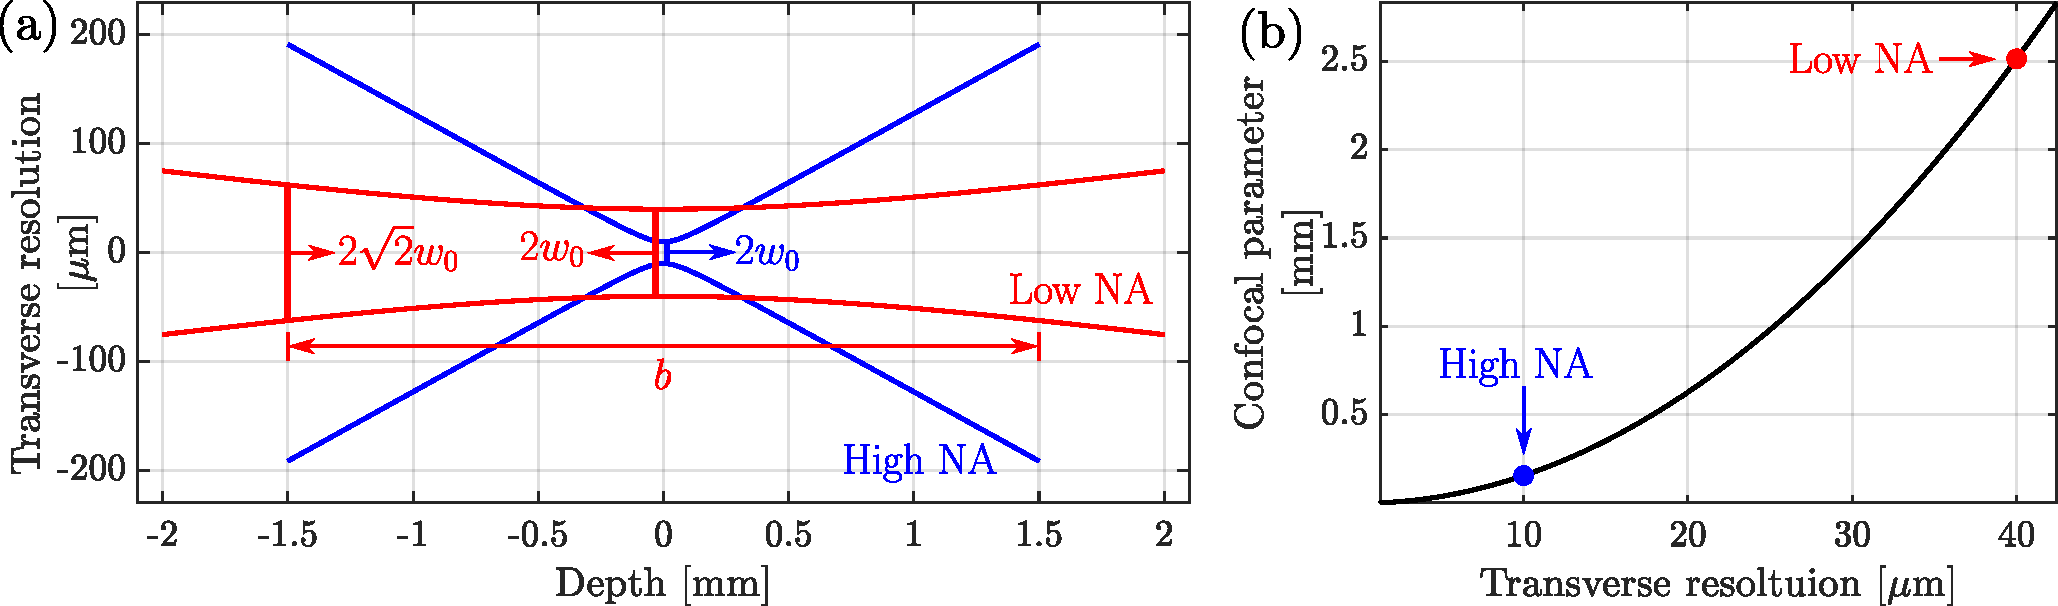
\includegraphics[width=\textwidth]{Figures/TheoreticalBasis/ConfocalScan.pdf}
    \caption[Illustration of confocal gating.]{Illustration of confocal gating for light with $\lambda_c = 1\mu$m. (a) Focused beam produced by two optical systems with relatively low and high NA. (b) Relation between confocal parameter and transverse resolution.}
    \label{fig:ConfocalScan}
\end{figure}

With this qualitative description of the resolution-DoF--trade-off, it is possible now to analyze how this impacts the acquired complex signal.

\subsection{Forward model}

This section presents the forward model (FM) that relates the measured OCT signal to the sample structure considering the effect of the optical system using a model for the image formation process. In the FM, the propagation of the Gaussian probe beam is taking into consideration to derive an expression for the interference signal that also considers the effect of confocal scan~\cite{Ralston2006_Inverse, Ralston2006_NonParaxial}. From Fourier optics theory, the acquired signal $S(x,y; k)$ for wavenumber $k$ at transverse coordinates $(x,y)$ can be modelled as $S(x,y; k)= h(x,y,z; k)\otimes\eta(x,y,z)$, that is the convolution (denoted by $\otimes$) of the system point-spread function (PSF) $h(x,y,z; k)$ with the scattering potential of the sample $\eta(x,y,z)$~\cite{Davis2007_Nonparaxial},
\begin{equation}\label{eq:conv}
    S(x,y; k) = \iiint h(x-x', y-y', z'; k) \eta(x',y',z') \text{d}x' \text{d}y' \text{d}z'
\end{equation}
where the integration over $z'$ indicates that light is captured simultaneously for all depths, as occurs in Fourier domain detection. The PSF $h(x,y,z; k)$ can be expressed as the product of the incident and detection complex probe beams $g_i(x,y,z;k)$ and $g_d(x,y,z;k)$ respectively, but given that OCT is based on a reflection (double-pass) geometry, the incident and collection beams are identical to $g(x,y,z;k)$, hence~\cite{Ralston2006_Inverse}
\begin{equation}\label{eq:PSF1}
    h(x,y,z; k) =k^2|A(k)|^2g^2(-x, -y, z; k),
\end{equation}
where $|A(k)|^2$ is the power spectral density and the inversion of lateral coordinates $(x,y)$ is due to the reflection geometry.

To derive a model for the probe beam $g(x,y,z;k)$, consider that the beam at the focal plane $z=z_0$ and transverse coordinate $\mathbf{r_0} = (x,y,z_0)$ is a normalized Gaussian probe beam
\begin{equation}\label{}
    g_0(\mathbf{r_0}; k) = \frac{1}{2\pi w_0^2(k)}e^{-\mathbf{r_0}^2/[2w_0^2(k)]},
\end{equation}
with waist radius $w_0(k) = \alpha / k$ for wavenumber $k$ and $\alpha = \pi/\text{NA}$. Using plane-wave decomposition with transverse frequency coordinate $\mathbf{q} = (q_x, q_y, 0)$, the beam at $\mathbf{r} = (x, y, z)$ in any plane $z$ is described as~\cite{Ralston2006_Inverse}
\begin{equation}\label{}
    g(\mathbf{r}; k) = \frac{1}{(2\pi)^2} \iint e^{i(z-z_0)\sqrt{k^2 - q^2}} e^{-q^2\alpha^2/2k^2} e^{i\mathbf{q}\cdot\mathbf{r}} \text{d}^2q
\end{equation}

Using Eqs.~\ref{eq:conv} and \ref{eq:PSF1}, it is possible to model the measured OCT interference signal taking into consideration the beam distribution, as explained in detail in Refs.~\cite{Ralston2006_Inverse, Marks2006_Inverse}, by means of the expression
\begin{equation}\label{eq:FM}
    S(\mathbf{r'}; k) = \frac{A(k)}{(2\pi)^2 k} \iiint f^2(\mathbf{r}-\mathbf{r'}; k) \eta(\mathbf{r}) \text{d}^2r \text{d}z,
\end{equation}
where the term $f^2(\mathbf{r}; k)$ is given by
\begin{equation}\label{eq:f^2}
    f^2(\mathbf{r}; k) = \frac{1}{8\pi^2}\left(\frac{\alpha^2}{k^2}+\frac{iz}{k}\right)^{-1} \iint e^{-q^2\alpha^2/4k^2} e^{iz\sqrt{4k^2-q^2}} e^{-i\mathbf{q}\cdot \mathbf{r}} \text{d}^2q.
\end{equation}

To understand Eq.~\ref{eq:FM}, note that $\mathbf{r'}=(x',y',z_0)$ is the instantaneous transverse position of the probe beam during a raster scan. The signal $S(\mathbf{r'},k)$ measured for the instantaneous wavenumber $k$ when the beam is located at the instantaneous position $\mathbf{r'}$ \textbf{is the contribution of all point scatterers in the sample weighted by the function $f^2(\mathbf{r}-\mathbf{r'}; k)$}, and scaled by a value proportional to the light source intensity for k, $A(k)$. Finally, a Fourier transform of $S(\mathbf{r'}; k)$ with respect to $k$ yields the depth-dependent signal $S(\mathbf{r'}, z)$. In regard to $f^2(\mathbf{r}-\mathbf{r'}; k)$, the factor $\frac{1}{8\pi^2}\left(\frac{\alpha^2}{k^2}+\frac{iz}{k}\right)^{-1}$ can be considered as a depth-dependent signal-loss factor that describes the signal reduction far from the focal plane, $e^{-q^2\alpha^2/4k^2}$ is related to the Fourier spectrum of the Gaussian beam, the factor $e^{iz\sqrt{4k^2-q^2}}$ encompasses both the interference and the PSF broadening effect, responsible of the signal blurring, and last factor $e^{-i\mathbf{q}\cdot \mathbf{r}}$ is the Fourier transform kernel as Eq.~\ref{eq:f^2} is actually a Fourier integral.

To illustrate the forward model, Figure~\ref{fig:FM1} shows an example of an OCT B-scan image simulated using Eq.~\ref{eq:FM}. For this purpose, a collection of $128$ point scatterers with random positions where defined within an axial and lateral field of view (FoV) of $820\times 450~\mu$m as depicted in Fig.~\ref{fig:FM1}(a). The light source have $\Delta\lambda=150$~nm and $\lambda_c=1.310~\mu$m providing an axial resolution of $\delta z=5~\mu$m. The numerical aperture is NA $= 0.25$, a relatively high value, resulting in lateral resolution $\delta x=5~\mu$m throughout a depth of field of $b=30~\mu$m, producing the Gaussian beam shown in Fig.~\ref{fig:FM1}(b), where the focal plane is clearly located at $z_0=0$. To generate the simulated OCT image shown in Fig.~\ref{fig:FM1}(c), the location of the Gaussian beam is changed iteratively, and in each location the contribution of all point scatterers weighted by $f^2(\mathbf{r}-\mathbf{r'}; k)$ is computed using Eq.~\ref{eq:FM}. At the $n$-th iteration, the location of the Gaussian beam is $\mathbf{r}'_m=(n\text{d}x - \frac{\Delta x}{2},0,z_0)$, where $\Delta x$ is the lateral FoV and $\text{d}x = 1.75~\mu$m is the sampling step which is smaller than Nyquist sampling $\delta x / 2$ in order to fulfill Nyquist theorem for correct sampling.

\begin{figure}[htb!]
    \centering
    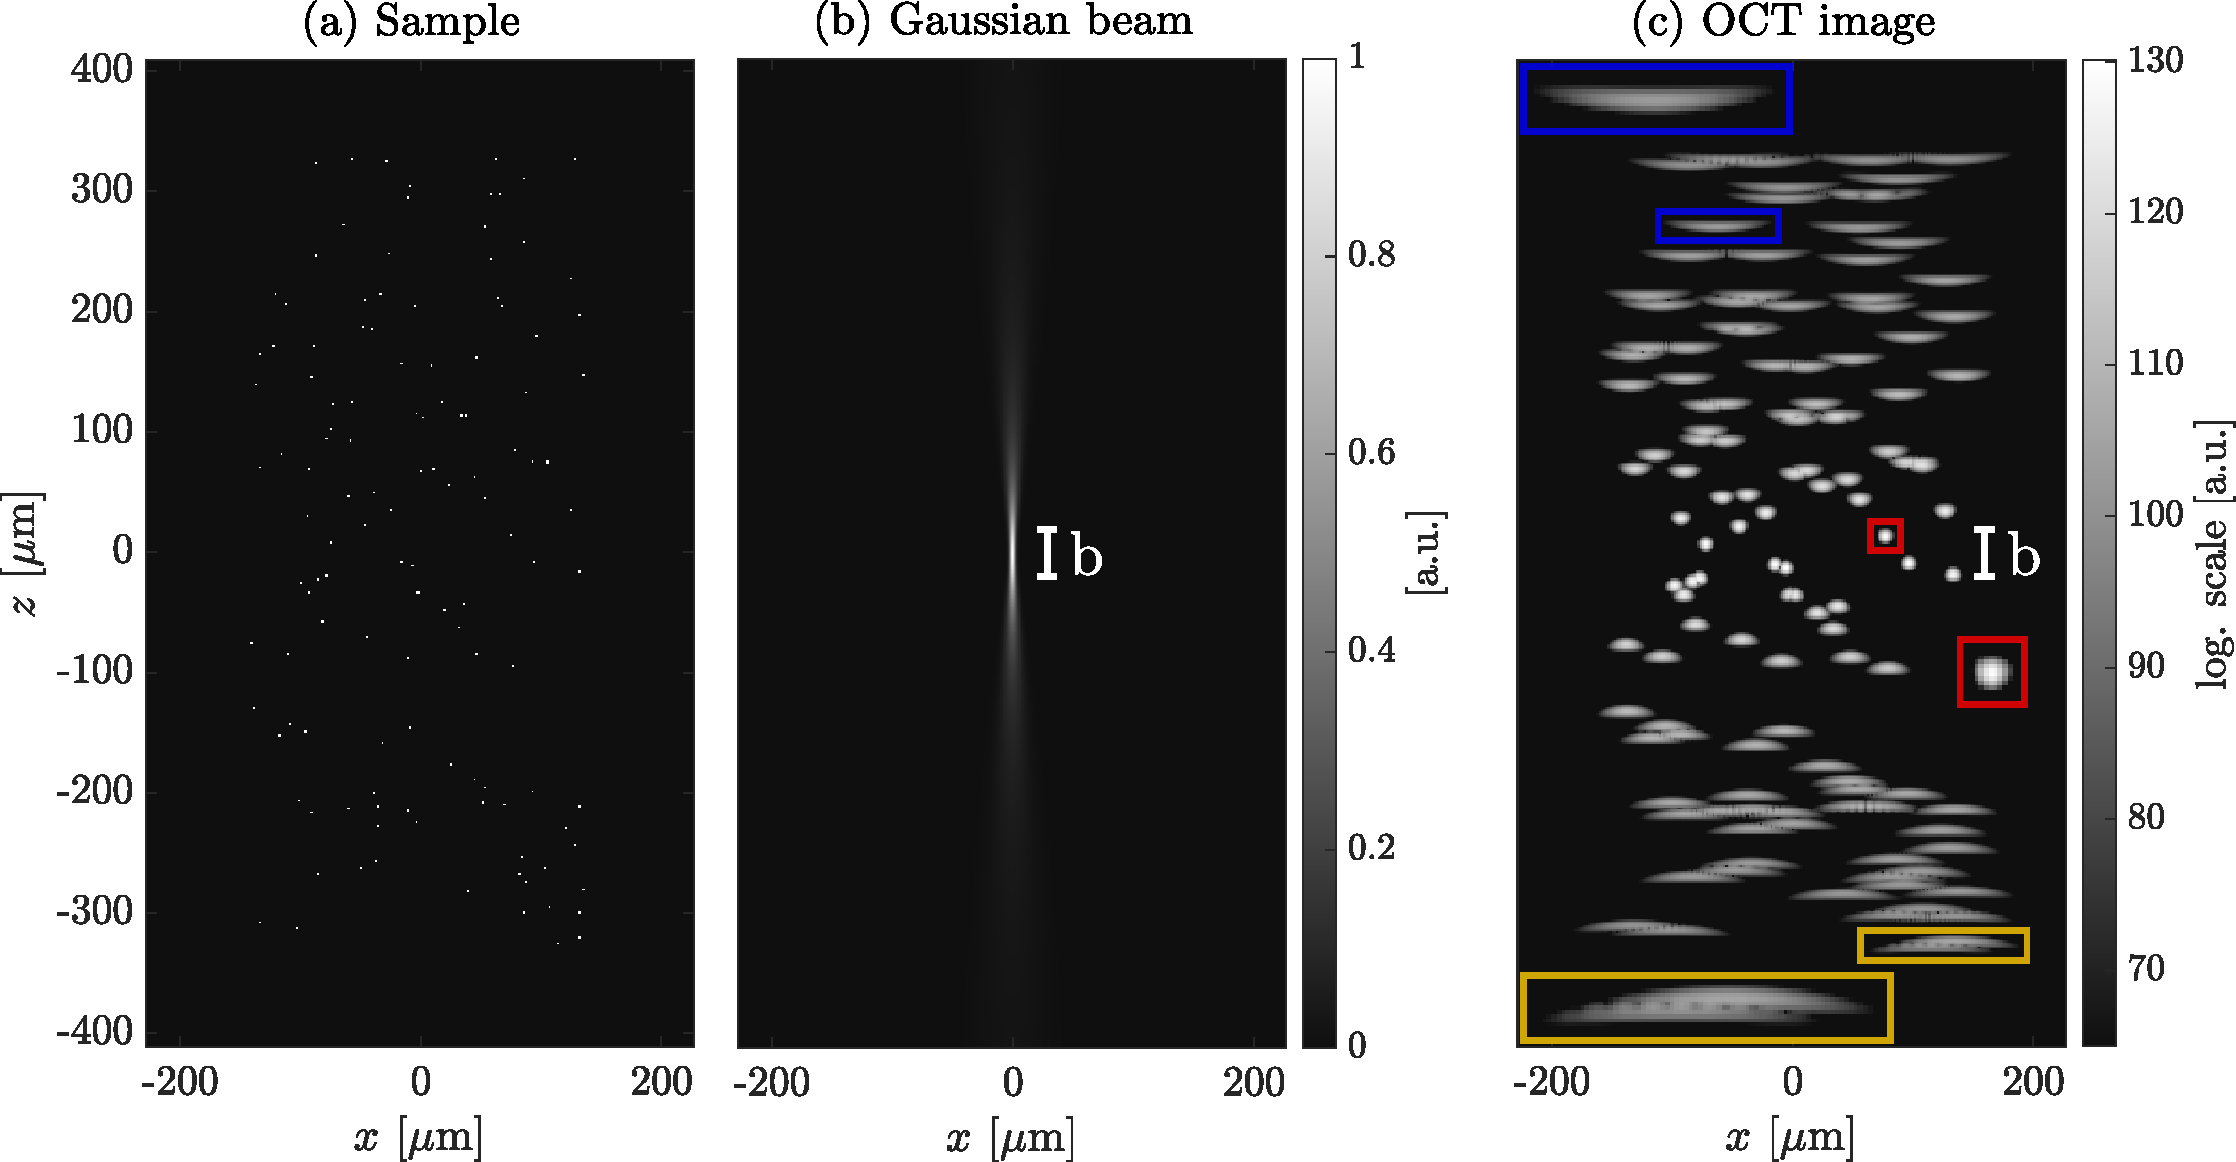
\includegraphics[width=\textwidth]{Figures/TheoreticalBasis/FM-HighNA.pdf}
    \caption[Simulation of an OCT image in high-NA regime.]{Simulation of an OCT image in high-NA regime. (a) Sample consisting of randomly located point scatterers, (b) Gaussian beam of the system with NA$=0.25$ and (c) OCT image simulated using the forward model, displayed in logarithmic scale.}
    \label{fig:FM1}
\end{figure}

The lateral blurring due to the convergence and divergence of the probe beam is evident in Fig.~\ref{fig:FM1}(c). Resolution within the confocal region marked as $b$ is diffraction-limited, so that point scatterers inside $b$ appear in focus, like the one inside the red rectangle, contrary to point scatterers away from the focal plane that appear blurred in the lateral axis as a consequence of beam size increase, such as the one in the blue rectangle. Note that superposition of signal from different point scatterers cause interference, like the two superimposed points in the yellow rectangle. When the number of point scatterers increases, random interference occurs and this phenomenon gives rise to speckle~\cite{Goodman2007_Speckle}.

It is important to remark that confocal effect is not restricted to the lateral axis. The factor $e^{iz\sqrt{4k^2-q^2}}$ in Eq.~\eqref{eq:f^2} can be written as $e^{izq_z(k, \mathbf{q})}$, where $q_z=\sqrt{4k^2-q^2}$ is the axial frequency coordinate of the object~\cite{Davis2007_Nonparaxial}. Because $q_z$ encompasses $k$ and $\mathbf{q}$, there is a mixing of the lateral and axial information that produce a coordinate warping, from the sample frequency coordinates $(q_x, q_y, q_z)$ to the signal frequency coordinates $(q_x, q_y, k)$~\cite{Ralston2006_Inverse}. As a consequence, there is an apparent object curvature away from the focal plane as observed in the yellow inset of Fig.~\ref{fig:FM1}(c). The signal warping occurs because the object axial frequency component $q_z$ is not measure directly but through the light wavenumber $k$~\cite{Fercher2003_Optical}. In other words, the object frequency content is in the $(q_x, q_y, q_z)$ space, but the measured signal is the $(q_x, q_y, \frac{1}{2}\sqrt{q_x^2 + q_y^2 + q_z^2})$ space. This phenomenon is significant in high NA regime, and for low-NA regime an approximation can be made to simplify the FM as will be discussed in the next section.

For a comparison between high and low NA regimes, Figure~\ref{fig:FM2} illustrates the result of imaging the same sample of Fig.~\ref{fig:FM1}(a) changing the NA to $0.1$, resulting in a lateral resolution of $ 12.5~\mu$m throughout a depth of field of $190~\mu$m. The Gaussian beam produced with this NA have a more constant beam size along depth, as shown in Fig.~\ref{fig:FM2}(b) in contrast to the previous NA used for Fig.~\ref{fig:FM1}(b). As a result, resolution loss away from the focal plane is less abrupt, at the expense of presenting a larger diffraction-limited spot size.

\begin{figure}[htb!]
    \centering
    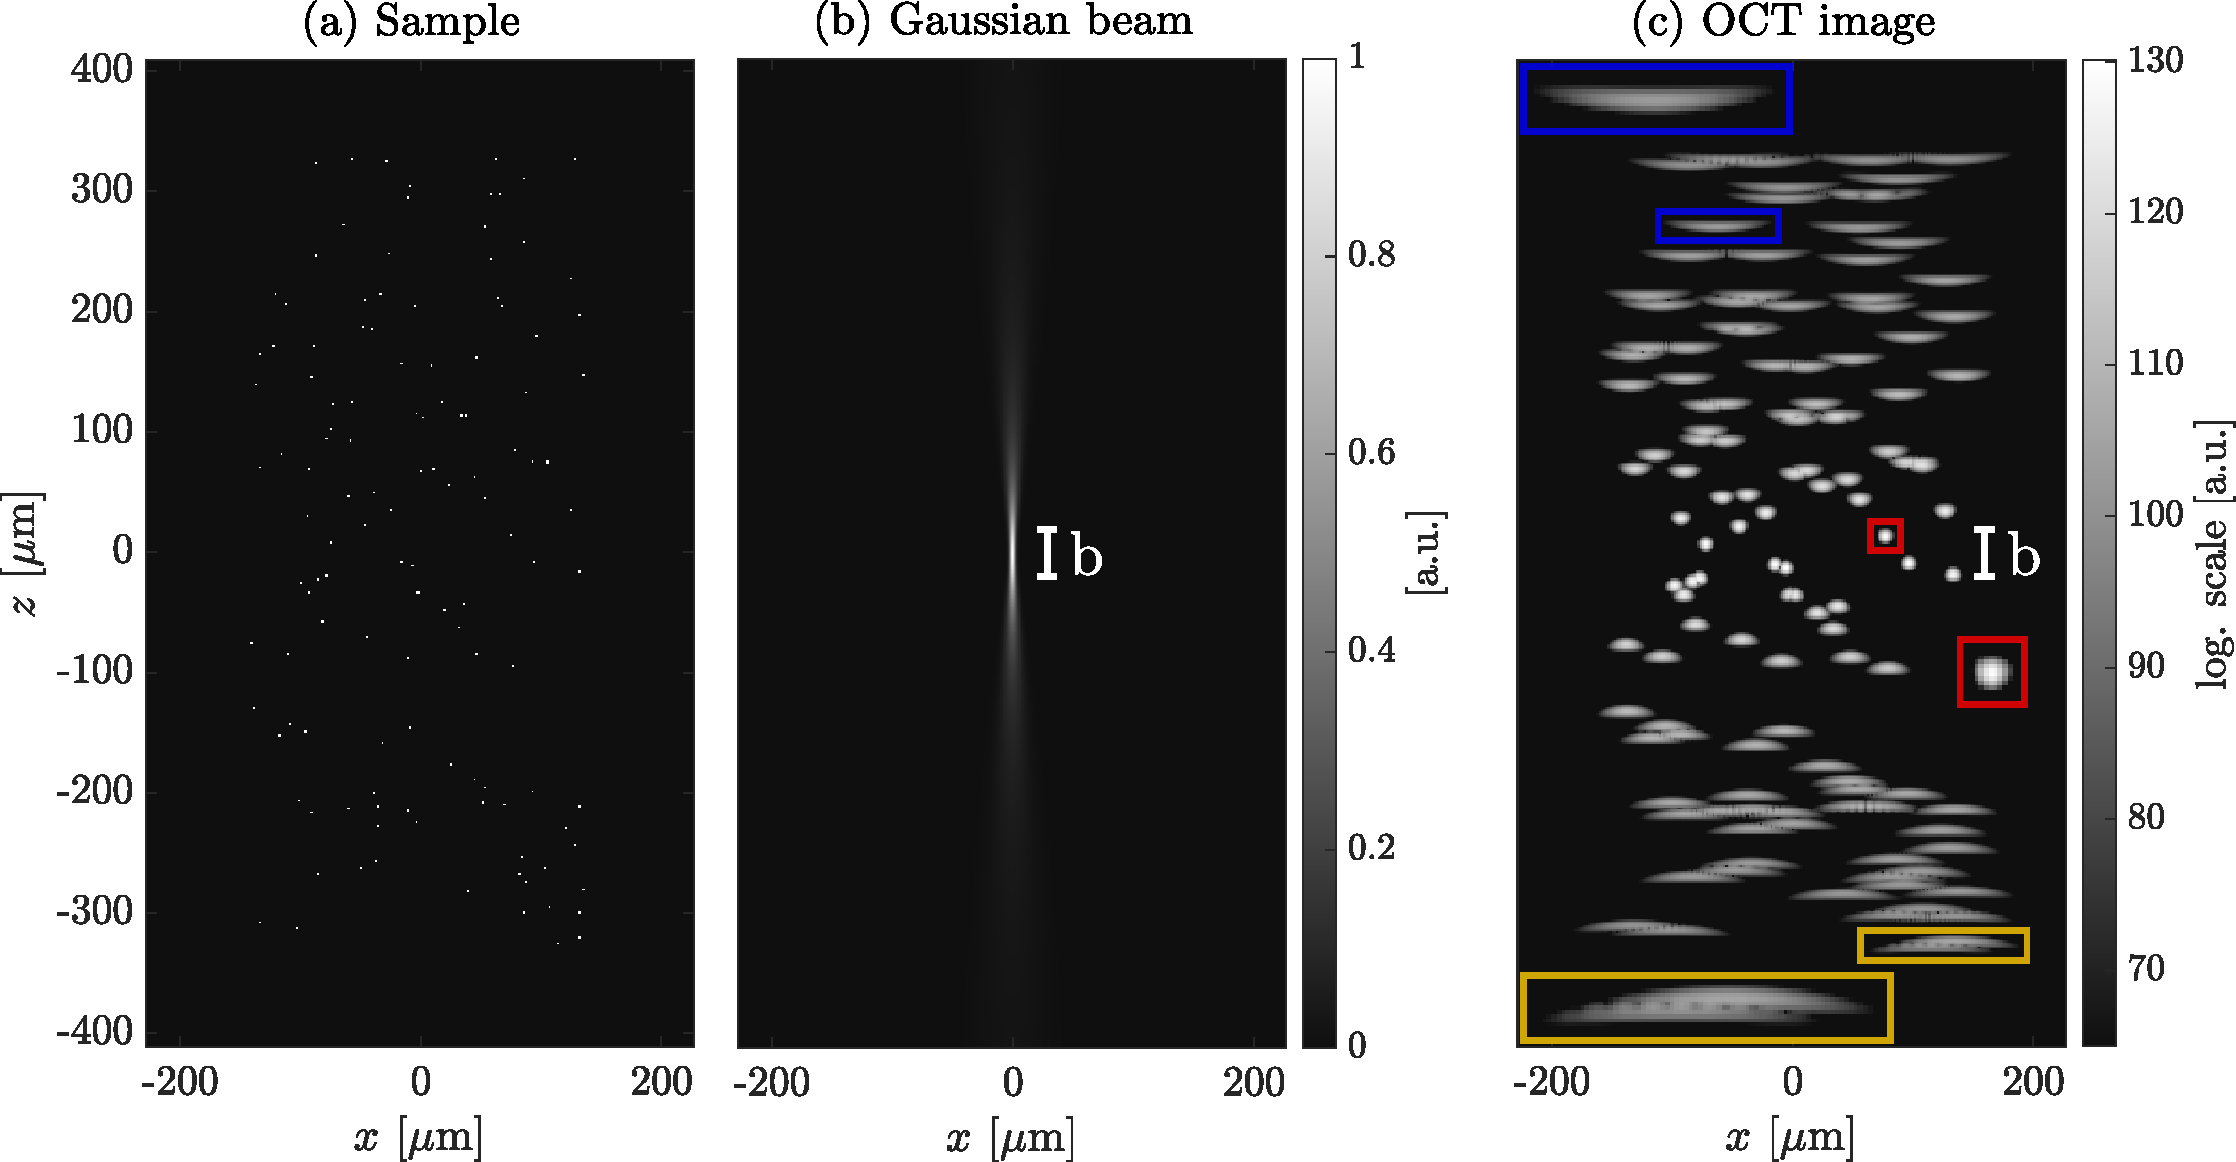
\includegraphics[width=\textwidth]{Figures/TheoreticalBasis/FM-LowNA.pdf}
    \caption[Simulation of an OCT image in low-NA regime.]{Simulation of an OCT image in low-NA regime. (a) Sample consisting of randomly located point scatterers, (b) Gaussian beam of the system with NA$=0.1$ and (c) OCT image simulated using the forward model, displayed in logarithmic scale.}
    \label{fig:FM2}
\end{figure}

% \iffalse Eq.~\ref{eq:conv} can be simplified in Fourier domain by invoking the convolution theorem and denoting the 2D Fourier transform over coordinates $(u, v)$ as $\text{FT}_{u,v}\{\cdot\}$,
% \begin{equation}\label{eq:convFT}
%     \hat{S}(q_x, q_y; k) = \int \hat{h}(q_x, q_y, z'; k) \hat{\eta}(q_x, q_y, z') dz'
% \end{equation}
% where $\hat{S} = \text{FT}_{x,y}\{S\}$, $\hat{h} = \text{FT}_{x,y}\{h\}$, $\hat{\eta} = \text{FT}_{x,y}\{\eta\}$, and $(q_x,q_y)$ are spatial frequency coordinates.

% The PSF can be expressed as the product of the incident and detection complex probe beams, and given that OCT is based on a reflection (double-pass) geometry, the incident and collection beams are identical to $\sqrt{\mu_r}k|A(k)|g(x,y,z;k)$, where $\mu_r$ is the beam splitting power ratio, $|A(k)|^2$ is the power spectral density, and $g(x,y,z; k)$ is the focused beam produced by an input collimated beam at the back focal length of the optical system, thereby
% \begin{equation}\label{eq:PSF1}
%     h(x,y,z; k) = \mu_rk^2|A(k)|^2g^2(-x, -y, z; k),
% \end{equation}
% where the inversion of lateral coordinates $(x,y)$ is due to the reflection geometry. 

% A plane wave decomposition of the focused probe beam yields~\ref{}
% \begin{equation}~\label{eq:planewavedecomp}
%     g(x,y,z ;k) = \frac{-i}{2\pi}\iint \frac{G(q_x, q_y, k)}{k_z}e^{i(q_xx+q_yy+k_zz)} dq_xdq_y,
% \end{equation}
% in terms of the generalized pupil function of the optical system $G(q_x, q_y, k)$, the object spatial frequencies $(q_x, q_y)$ and with $k_z(q_x, q_y) = \sqrt{k^2 - q_x^2 - q_y^2}$ that results from considering the optical wave vector $\mathbf{k}=(q_x, q_y, k_z)$.

% The 2D Fourier transform over coordinates $(q_x, q_y)$ of Eq.~\ref{eq:planewavedecomp}, $\hat{g} =  \text{FT}_{x,y}\{g\}$, results in
% \begin{equation}\label{eq:gFT}
%     \hat{g}(q_x, q_y, z; k) = -i2\pi\frac{G(q_x, q_y; k)}{k_z(q_x, q_y)}e^{izk_z(q_x, q_y)}
% \end{equation}

% Now, computing the 2D Fourier transform over coordinates $(q_x, q_y)$ of Eq.~\ref{eq:PSF1} and using the convolution theorem, note that the transverse transfer function $\hat{h} \propto \hat{g} \otimes\hat{g}$ and it can be expressed using Eq.~\ref{eq:gFT} as
% \begin{align}\label{eq:hFT}
%     \hat{h}(-q_x, -q_y, z; k) = -4\pi^2\mu_rk^2|A(k)|^2  &\iint \frac{G(q_x', q_y'; k)}{k_z(q_x', q_y')} \frac{G(q_x-q_x', q_y-q_y'; k)}{kz(q_x-q_x', q_y-q_y')}... \nonumber\\
%     &\times e^{-izk_z(q_x', q_y')}e^{-izk_z(q_x-q_x', q_y-q_y')}dq_x'dq_y'
% \end{align}

% To solve the integral in Eq.~\ref{eq:eq:hFT} it is possible to consider two complementary situations; near- and far-from-focus regimes. Recalling that $z=0$ at the focal plane, the far-from-focus regime is valid outside the DoF where effect of defocus is significant, where $z$ becomes large hence the phase term $|zk_z(q_x',q_y')|$ causes a rapid oscillation of the exponential term. This consideration allows to make use of the method of stationary phase~\ref{} which applies for integrals containing a rapidly oscillating complex exponential, such that the solution of the integral is found by evaluating the integral in the stationary point~\ref{}, that is, the point at which the argument of the complex exponential has zero gradient. The approximation of integral in Eq.\ref{eq:hFT} using the stationary point $(q_x', q_y') = (q_x/2, q_y/2)$ is
% \begin{equation}\label{eq:hFT_fff}
%     \hat{h}(-q_x, -q_y, z; k) \approx \frac{i4\pi}{-z}\mu_rk|A(k)|^2G^2\left(\frac{q_x}{2}, \frac{q_y}{2}; k\right)e^{-i2zk_z(\frac{q_x}{2}, \frac{q_y}{2})}.
% \end{equation}

% This expression shows explicit the amplitude and phase of the transverse transfer function of the system. The factor of $i=e^{i\frac{\pi}{2}}$ is equivalent to a phase of $\frac{\pi}{2}$ that is known as Gouy phase shift and it is characteristic of focused Gaussian beams~\ref{}. Decaying factor $1/z$ represents the signal decay with distance from focal plane that explains the loss of signal strength outside the DoF. In addition to the previous term, the other phase-dependent term is the phase factor that is responsible for the degradation of transverse resolution with increasing distance to the focal plane.

% For the near-focus regime, consideration to apply the method of stationary phase to solve the integral in Eq,~\ref{eq:hFT} is not longer valid. In this case, $z$ is small hence the phase term $|zk_z(q_x',q_y')|$ oscillates slowly and the term $G(q_x', q_y'; k)$ can be considered narrowly peaked compared to the slow oscillation of the exponential term, and this can be used to derive an approximation solution~\ref{}, however, the derivation is rather extensive as explained in detail in Ref.~\ref{} and superfluous in this context considering that inside the DoF defocus correction is unnecessary when compared to the far-from-focus regime.

% To finally derive the forward model for the far-from-focus regime, the transfer function of the system in Eq.~\ref{eq:hFT_fff} is replaced in Eq.~\ref{eq:convFT} to obtain
% \begin{equation}\label{eq:SFT}
%     \hat{S}_F(q_x, q_y; k) =  H_F(q_x, q_y; k)\int \frac{\tilde{\eta}(q_x, q_y, z')}{-z'}e^{-i2z'k_z(\frac{q_x}{2}, \frac{q_y}{2})} dz'.
% \end{equation}
% where $H_F(q_x, q_y; k) = i4\pi\mu_r k |A(k)|^2 G^2(-\frac{q_x}{2}, -\frac{q_y}{2}; k)$ is the depth-independent component of $\hat{h}$. Eq.~\ref{eq:SFT} is in the form of a Fourier transform with conjugate coordinates $z'$ and $2k_z(\frac{q_x}{2}, \frac{q_y}{2})$ and filtered by $H_F$. In fact, it has been proven that the forward model for the near-focus regime follow the same form that the forward model for far-from-focus, except that the Gouy phase shift and the decaying term $-1/z$ are not present and the depth-independent component of $\hat{h}$, denoted by $H_N(q_x, q_y; k)$, follows a slightly different functional form as can be seen in Ref.~\ref{}. Therefore, an unified approximate forward model for near- and far-from-focus regimes can be expressed in frequency domain as
% \begin{equation}\label{eq:FM}
%     \hat{S}(q_x, q_y; k) = H(q_x, q_y; k)\doublehat{\eta_a}(q_x, q_y, q_z)
% \end{equation}
% where $\doublehat{\eta_a}(q_x, q_y, q_z) = \text{FT}_{x,y,z}\{\rho(z)\eta(x,y,z)\}$ is the 3D Fourier transform of the attenuated scattering potential with spatial frequency coordinates $(q_x, q_y, q_z)$ where $q_z = -2\sqrt{k^2 - \left(\dfrac{q_x}{2}\right)^2 - \left(\dfrac{q_y}{2}\right)^2}$, and with the unified functions $H$ and $\rho$ given by
% \begin{equation}
% H(q_x, q_y; k) = 
% \begin{cases}
%     H_N(q_x, q_y; k)~~~\text{for}~~~|z| \ll z_R, \\
%     H_F(q_x, q_y; k)~~~\text{for}~~~|z| \gg z_R,
% \end{cases}
% \end{equation}
% \begin{equation}\label{eq:rhoz}
% \rho(z) = 
% \begin{cases}
%     ~1~~~~~\text{for}~~~|z| \ll z_R, \\
%     -\dfrac{1}{z}~~~\text{for}~~~|z| \gg z_R.
% \end{cases}
% \end{equation}

% The forward model in Eq.~\ref{eq:FM} is a one-to-one mapping of the frequency distribution of the measured signal $\hat{S}$ and the frequency distribution of the attenuated scattering potential $\doublehat{\eta}_a$, with an additional filtering $H$ and with a coordinates conversion from the sample coordinates $(q_x, q_y, q_z)$ to the signal coordinates $(q_x, q_y, k)$, and this is responsible for the sample scattering potential appearing defocused in the acquired signal. The coordinate conversion causes a signal warping as a consequence of the indirect measurement of the scattering potential using an optical beam with particular wavenumber $k$.

% To illustrate this, consider two point reflectors, one in the focal plane of the light probe and the other far from the focal plane as depicted in  Figure~\ref{}. Scattering follows the scattering vector relationship $\mathbf{q} = \mathbf{k}_{out} - \mathbf{k}_{in}$ that is a consequence of the momentum conservation, where $\mathbf{q}$ is the three-dimensional spatial frequency vector of the sample that is being measured and $\mathbf{k}_{out}$, $\mathbf{k}_{in}$ are wave vectors of the scattered and incident light, respectively. Input and scattered wavenumbers are within an acceptance angular range determined by the numerical aperture, describing what is known in diffraction tomography as an \textit{Ewald sphere}~\ref{}.

% For the point in the focal plane, the whole angular view is collected in a single scan, therefore resolution is diffraction-limited. Also, note that a large NA provides a wider angular scan thus more frequencies components $\mathbf{q}$ of the sample are probed increasing lateral resolution.

% For a point far from the focal plane, the acceptance angle becomes narrow, hence the frequency content $\mathbf{q}$ of the sample that can be probed in a single scan is smaller and resolution is decreased. Nonetheless, scanning the beam along the transverse coordinates increases the effective acceptance angle and it is possible to collected the frequency content of the sample even far-from-focus but along the sequential lateral scans, not in a single scan as for a point in the focal plane. This fact is related to the signal warping causing blurring of far-from-focus structures. For far-from-focus regime, $\mathbf{k}_{out}\approx - \mathbf{k}_{in}$ thus the measured frequency is $\mathbf{q} \approx -2 \mathbf{k}_{in}$, and the square magnitude yields the relation $4k = q_x^2 + q_y^2 + q_z^2$, that is the same obtained in the coordinate mapping of the forward model in Eq.~\ref{eq:FM}.
% \fi


\section{Refocusing and computational aberration correction techniques in OCT}\label{CAC}

In the FM of Eq.~\ref{eq:FM}, the OCT signal $S$ is given by the sample potential $\eta$ modified by the system funcion $f^2$~\cite{Marks2006_Inverse}. From this model, it is possible to computationally obtain an approximate scattering sample potential $\tilde{\eta}$ by correcting the undesired effects present in the acquired signal $S$, that so far is only defocus due to the beam propagation, but additional aberrations may also be considered with further extensions presented below. There are several computational aberration correction techniques, some are oriented to correct for defocus to provide focal resolution throughout all depths, and others are oriented to correct for other types of aberrations that depend on the specific imaging system or even on the sample itself, in addition to defocus, and they are explained in the following sections.

To retrieve an approximate scattering sample potential from the acquired signal it is necessary to invert the forward model, what is known as an inverse scattering problem~\cite{Ralston2006_Interferometric}. In simple words, the FM gives the backscattering signal produced for a given scattering potential, while the inverse model gives the scattering potential that produced a given backscattering signal, and the latter is the interest in CAC.

For the derivation of CAC techniques, it is convenient to introduce the forward model in Fourier domain~\cite{Liu2017_Computational}. To do so, the convolution theorem can be used to rewrite Eq.\eqref{eq:conv} as
\begin{equation}\label{eq:convFT}
    \hat{S}(q_x, q_y; k) = \int \hat{h}(q_x, q_y, z'; k) \hat{\eta}(q_x. q_y, z') \text{d}z'
\end{equation}
where $\hat{S}(q_x, q_y; k)=\text{FT}_{x,y}\{S(x,y;k)\}$, $\hat{h}(q_x, q_y, z; k)=\text{FT}_{x,y}\{h(x,y,z;k)\}$ is the depth-dependent frequency response of the PSF, and $\hat{\eta}(q_x, q_y, z)=\text{FT}_{x,y}\{\eta(x,y,z)\}$. Using an asymptotic approximation for the far-from-focus and near-focus cases~\cite{Davis2007_Nonparaxial}, Eq.~\eqref{eq:convFT} can be simplified to
\begin{equation}\label{eq:FMft}
    \hat{S}(q_x, q_y; k) = H(q_x, q_y; k) \int \hat{\eta}(q_x. q_y, z') e^{iz'\sqrt{4k^2-q^2}} \text{d}z'
\end{equation}
where $H(q_x, q_y; k)$ is the space-invariant axial and lateral frequency response of the PSF, that is directly related to the optical transfer function of the system. In Eq.\eqref{eq:convFT}, a Gaussian beam is not assumed, contrary to the derivation of the FM in Eq.~\eqref{eq:FM}, so that $H(q_x, q_y; k)$ is a general function that may describe any aberration and not only defocus. Computational aberration correction makes use of the FM in frequency domain to reconstruct an approximate sample scattering potential~\cite{Liu2017_Computational}.

In the notation used here, the tilde accent $\tilde{\ }$ is used to denote that a quantity is an numerical estimation of the true quantity. For instance $\tilde{\eta}$ is an estimation of $\eta$ using any of the CAC models presented above.

Furthermore, given that in practical terms computational approaches operate sampled variables rather than continuous variables, it is useful to define discrete notation to refer to the sampled counterparts of the ideally continuous variables. Hereafter, discrete indexes ($m, n, l$) are used as discrete counterparts of continuous coordinates $(x,y,z)$, respectively. For instance, $S(m,n,l)$ is the discrete counterpart of the signal $S(x,y,z)$, which in some cases will be written as $S_{m,n,l}$ for simplicity. In general, mathematical models will be described in continuous notation, and discrete notation will be used exclusively in equations that are intrinsically discrete.

\subsection{Interferometric synthetic aperture microscopy}

Interferometric synthetic aperture microscopy (ISAM) is a solution to the inverse scattering problem in OCT~\cite{Ralston2006_Interferometric, Ralston2007_Interferometric}, and actually it is very similar to procedures used in synthetic aperture radar (SAR)~\cite{Cafforio1991_SAR} and from this similarly arises the name ISAM. Eq.~\eqref{eq:FMft} can be considered as a Fourier integral with conjugate coordinates $z'$ and $q_z=\sqrt{4k^2-q^2}$, thus it is possible to write
\begin{equation}\label{eq:preISAM}
    \hat{S}(q_x, q_y; k) = H(q_x, q_y; k) \doublehat{\eta}(q_x. q_y, q_z)
\end{equation}
where $\doublehat{\eta} = \text{FT}_{x,y,z}\{\eta(x,y,z)\}$ is the 3D Fourier transform of the sample scattering potential. Eq.~\ref{eq:preISAM} is a one-to-one mapping between $\hat{S}$ and $\doublehat{\eta}$, contrary to convolution equation that is an all-to-all mapping between $S$ and $\eta$. The principle of operation of ISAM is to re-sample the Fourier spectrum of the acquired signal $S(x, y; k)$ in order to revert the coordinate warping, thereby the approximate scattering sample potential $\tilde{\eta}(x,y,z)$ can be expressed as~\cite{Ralston2007_Interferometric}

\begin{equation}\label{eq:ISAM}
    \tilde{\eta}(x,y,z) = \frac{1}{\rho(z)} \text{FT}^{-1}_{q_x,q_y.q_z}\left\{\big[H^{-1}(q_x, q_y; k) \hat{S}(q_x, q_y; k)\big]\bigg|_{k = \frac{1}{2}\sqrt{q_x^2 + q_y^2 + q_z^ 2}}\right\}.
\end{equation}
where $\rho(z) = -1/z$ countervails signal loss when far from focus. Eq.~\ref{eq:ISAM} consist in several steps; 1) computing the Fourier transform of the acquired signal along transverse spatial coordinates, 2) re-maping coordinates from $k$ to $q_z$ using the relation $k = \frac{1}{2}\sqrt{q_x^2 + q_y^2 + q_z^2}$, known as the Stolt mapping~\cite{Stolt1978_Mitigation}, and then 3) computing the three-dimensional inverse Fourier transform $\text{FT}^{-1}\{\cdot\}$. For ISAM, an ideal Gaussian beam is generally assumed, so that $H^{-1}$ is a weighting factor that will not introduce significant image distortion, thus it is usually set to unity. Normalization using $1/\rho(z)$ is not appropriate in practical terms to compensate for signal loss away from focal plane, thus it is commonly omitted or replaced with other depth normalization function.

\iffalse
ISAM reconstruction is illustrated in Figure~\ref{fig:IM1} for the high-NA case of the simulated data in Fig.~\ref{fig:FM1}. The ISAM reconstruction shown in Fig.~\ref{fig:IM1}(c) exhibit diffraction-limited resolution throughout all depths, and the major drawback present is the signal reduction, noticeable in points far from focal plane appearing dimmer than those in the focal plane.

ISAM reconstruction is illustrated in Figure~\ref{fig:ISAM} for the case of the simulated data of sample with two point reflectors, one in the focal plane and the other above, outside the Rayleigh range. Note that point far-from-focus appears greatly blurred in Fig.~\ref{fig:ISAM}(a), because the curvature distortion of the frequency components in the Fourier spectrum as seen in Fig.~\ref{fig:ISAM}(b). ISAM resampling compensates the phase curvature as shown in Fig.~\ref{fig:ISAM}(d), yielding an approximate sample scattering potential with diffraction-limited resolution throughout depth, although intensity of the point outside the Rayleigh range is lower than that of the point in the focal plane.

\begin{figure}[htb!]
    \centering
    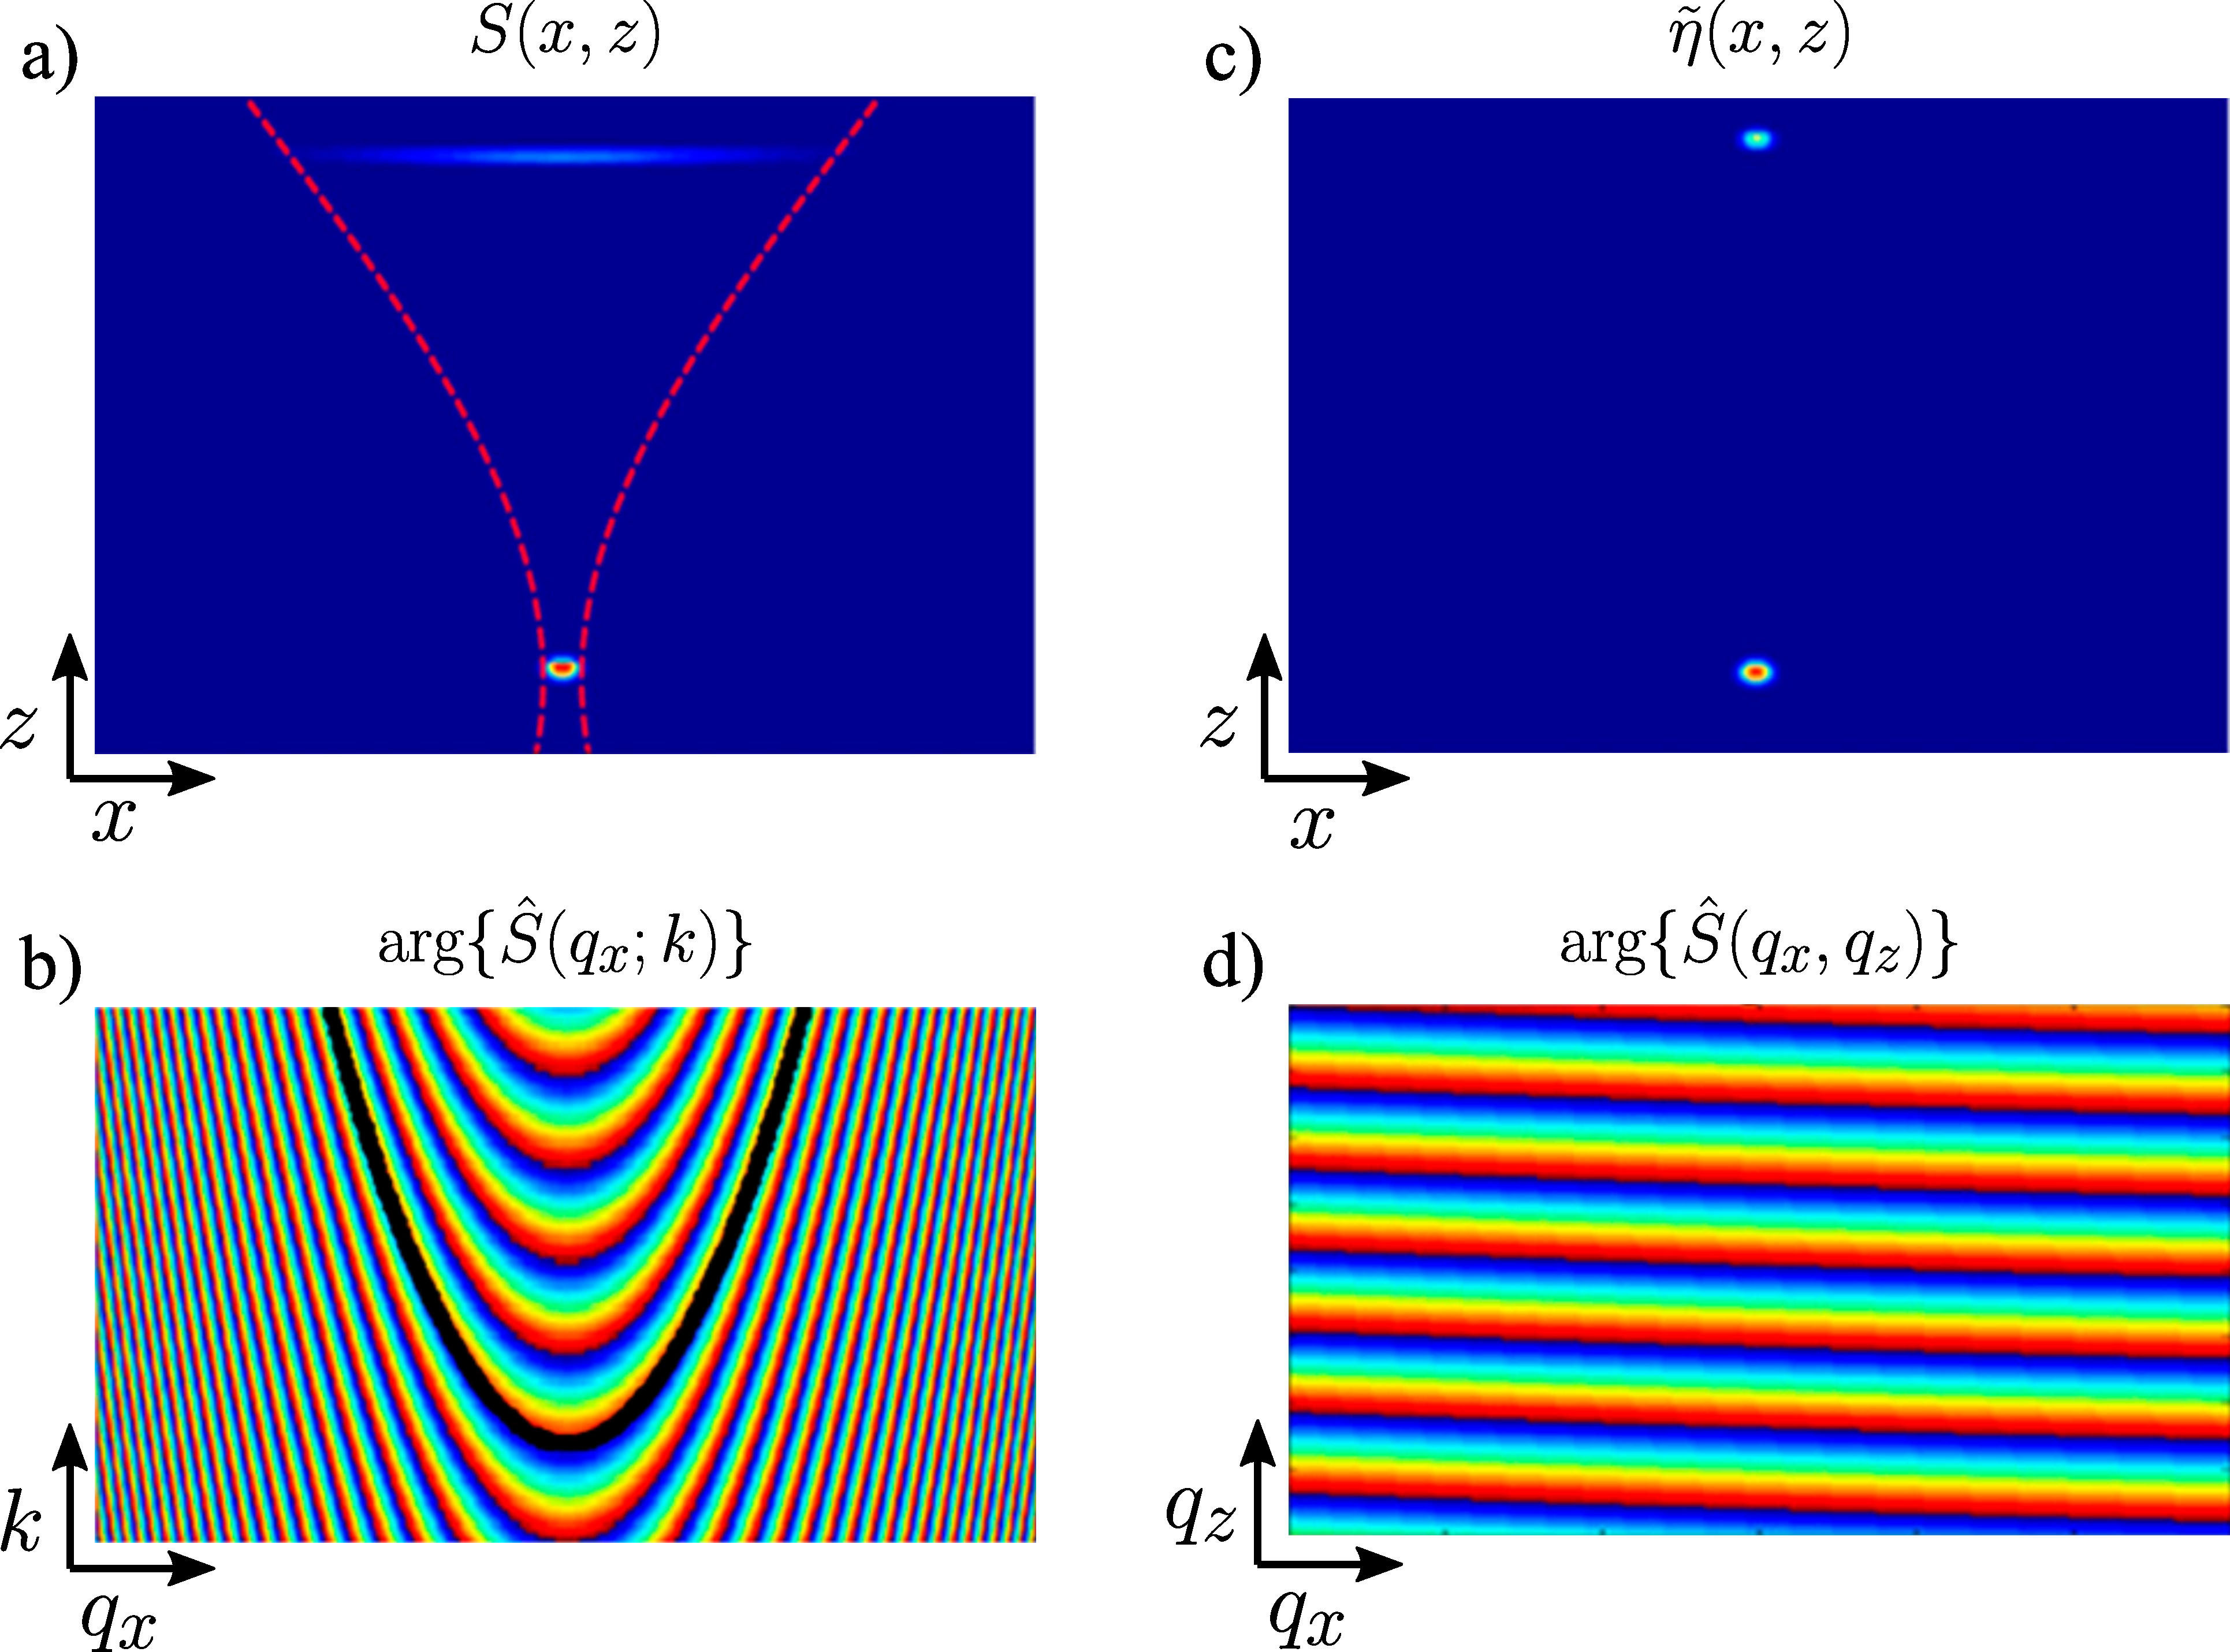
\includegraphics[width=.75\textwidth]{Figures/TheoreticalBasis/ISAM.pdf}
    \caption[Illustration of ISAM operation.]{Illustration of ISAM operation. (a) Acquired B-scan image, (b) phase map of its Fourier transform in $k$-space and (d) in $q_z$-space after re-sampling, yielding ISAM reconstruction in (c). Red line in (a) represents the distribution of the focused beam when positioned in the central Aline, and black line in figure (b) is an example of ISAM sampling curve. Figure adapted from Ref.~\ref{sudkamp}.}
    \label{fig:ISAM}
\end{figure}
\fi

ISAM, first proposed by Ralston et al.~\cite{Ralston2006_Interferometric}, has been used widely in the OCT community specially in high-resolution imaging where DoF is greatly reduced and computational correction of defocus is a key tool to extended the DoF~\cite{Liu2014_Computed, Boppart2015_Computational, Yi2019_Structure, Zysk2015_Intraoperative}, being the signal loss the major constrain. Extensions have been made to different imaging geometries and functional imaging, such as rotationally-scanned ISAM for endoscopic OCT~\cite{Marks2006_Inverse-1, Marks2006_Inverse}, and polarization-sensitive ISAM~\cite{Davis2007_Polarimetric}. Furthermore, the development of ISAM have enable real-time \textit{in vivo} visualization~\cite{Ralston2008_Realtime, Ralston2013_Interferometric, St.Marie2013_Robust}. 

\subsection{Digital refocusing}

ISAM reconstruction brings to focus all depths simultaneously, making use of the 3D frequency content of the tomogram. In relatively low numerical aperture systems (NA $<$ 0.15) the re-sampling curve approximates a linear path which means that frequency content in not spread along depth, hence a 2D correction in the transverse plane determined for each plane $z$ independently is sufficient~\cite{Yasuno2006_Noniterative, South2016_Computed} rather than a 3D correction as in ISAM. To isolate a single plane $z_d$, inverse Fourier transform along $k$ of Eq.\eqref{eq:FMft} is computed and evaluated at $z=z_d$,
\begin{equation}\label{eq:preDefocus}
    \hat{S}(q_x,q_y; z_d) = \int H(q_x, q_y; k) \int \hat{\eta}(q_x,q_y, z_d) e^{iz\sqrt{4k^2-q^2}} e^{-i2z_dk} \text{d}z\text{d}k.
\end{equation}
Replacing $k=k_c + k'$, being $k'$ the difference between $k$ and central wavenumber $k_c$, the term $(k'/k_c)^2$ is relatively small enough to be neglected, allowing to express $q_z=\sqrt{4k^2-q^2}$ under the paraxial approximation as~\cite{South2016_Computed}
\begin{equation}\label{eq:qzAprox}
    q_z = 2k_c - \frac{q^2}{4k_c} + 2k'.
\end{equation}

Replacing $q_z$ in Eq.\eqref{eq:preDefocus}, as well as using convolution theorem to rewrite Foruier integral along $k'$, it is possible to obtain~\cite{South2016_Computed}
\begin{align}\label{eq:preDefocus2}
    \hat{S}(q_x,q_y; z_d) &= \int H(q_x, q_y; k') \int \hat{\eta}(q_x,q_y, z_d) e^{iz(2k_c - q^2/4k_c + 2k')} e^{-i2z_d(k_c+k')} \text{d}z\text{d}k' \nonumber \\
    &= \int H(q_x, q_y; k') \int \hat{\eta}(q_x,q_y, z_d) e^{i2(z-z_d)k_c} e^{-izq^2/4k_c} e^{i2(z-z_d)k'} \text{d}z\text{d}k' \nonumber \\
    &= H(q_x, q_y; z_d) \otimes \left[ \int \hat{\eta}(q_x,q_y, z_d) e^{i2(z-z_d)k_c} e^{-izq^2/4k_c}  \delta(2z-2z_d) \text{d}z\right] \nonumber \\
    &= H(q_x, q_y; z_d) \otimes \left[ \hat{\eta}(q_x,q_y, z_d) e^{-iz_dq^2/4k_c}  \right]
\end{align}
where the convolution is performed along axial axis. The depth-dependent part of $Hq_x,q_y;z_d)$ is related to the axial PSF that can be approximated to a delta function, so that $H(q_x, q_y; z) \propto H(q_x, q_y)\delta(z-z_d)$, which can be replaced in Eq.~\eqref{eq:preDefocus2} to obtain its inverse Fourier transform along $\mathbf{q}$ as
\begin{equation}\label{eq:defocus}
    S(x, y; z_d) = \text{FT}^{-1}_{q_x, q_y}\left\{H(q_x, q_y)\hat{\eta}(q_x, q_y; z_d) e^{-iz_dq^2/4k_c}\right\},
\end{equation}

Eq.~\eqref{eq:defocus} is an expression with a form widely known in digital refocusing methods based on scalar diffraction models~\cite{Ralston2005_Deconvolution, Yu2007_Improved, Liu2009_Deconvolution} such as the Fresnel propagator~\cite{Yasuno2006_Noniterative}, where the exponential term is a quadratic phase term responsible of depth-varying defocus. A straightforward inversion of Eq.~\eqref{eq:defocus} provides an approximate refocused sample scattering potential by~\cite{South2016_Computed}
\begin{equation}\label{eq:refocus}
    \tilde{\eta}(x,y; z_d) = \text{FT}^{-1}_{q_x, q_y}\left\{H(q_x, q_y)\hat{S}(q_x, q_y; z_d) e^{iz_dq^2/4k_c}\right\},
\end{equation}
Similarly to ISAM, an ideal Gaussian beam can be assumed and $H$ is set to unity. Reconstruction using digital refocusing of Eq.\eqref{eq:refocus} is not complex and implementation is rather simple compared to ISAM, but there are conceptual differences with ISAM reconstruction. In digital refocusing, each depth is brought to focus independently, applying an appropriate quadratic phase term, whereas ISAM reconstruction restores the entire volume simultaneously re-sampling the signal in Fourier domain. More importantly, due to the paraxial approximation in Eq.\eqref{eq:qzAprox}, digital refocusing methods are valid only for low-NA regimes, where there is not coordinates warping that mixes lateral and axial information. Digital refocusing is illustrated in Figure~\ref{fig:IM2} for the low-NA case of the simulated data in Fig.\ref{fig:FM2}, and note that digital refocused image of Fig.~\ref{fig:IM2}(c) exhibit diffraction-limited resolution throughout all depth.

\begin{figure}[htb!]
    \centering
    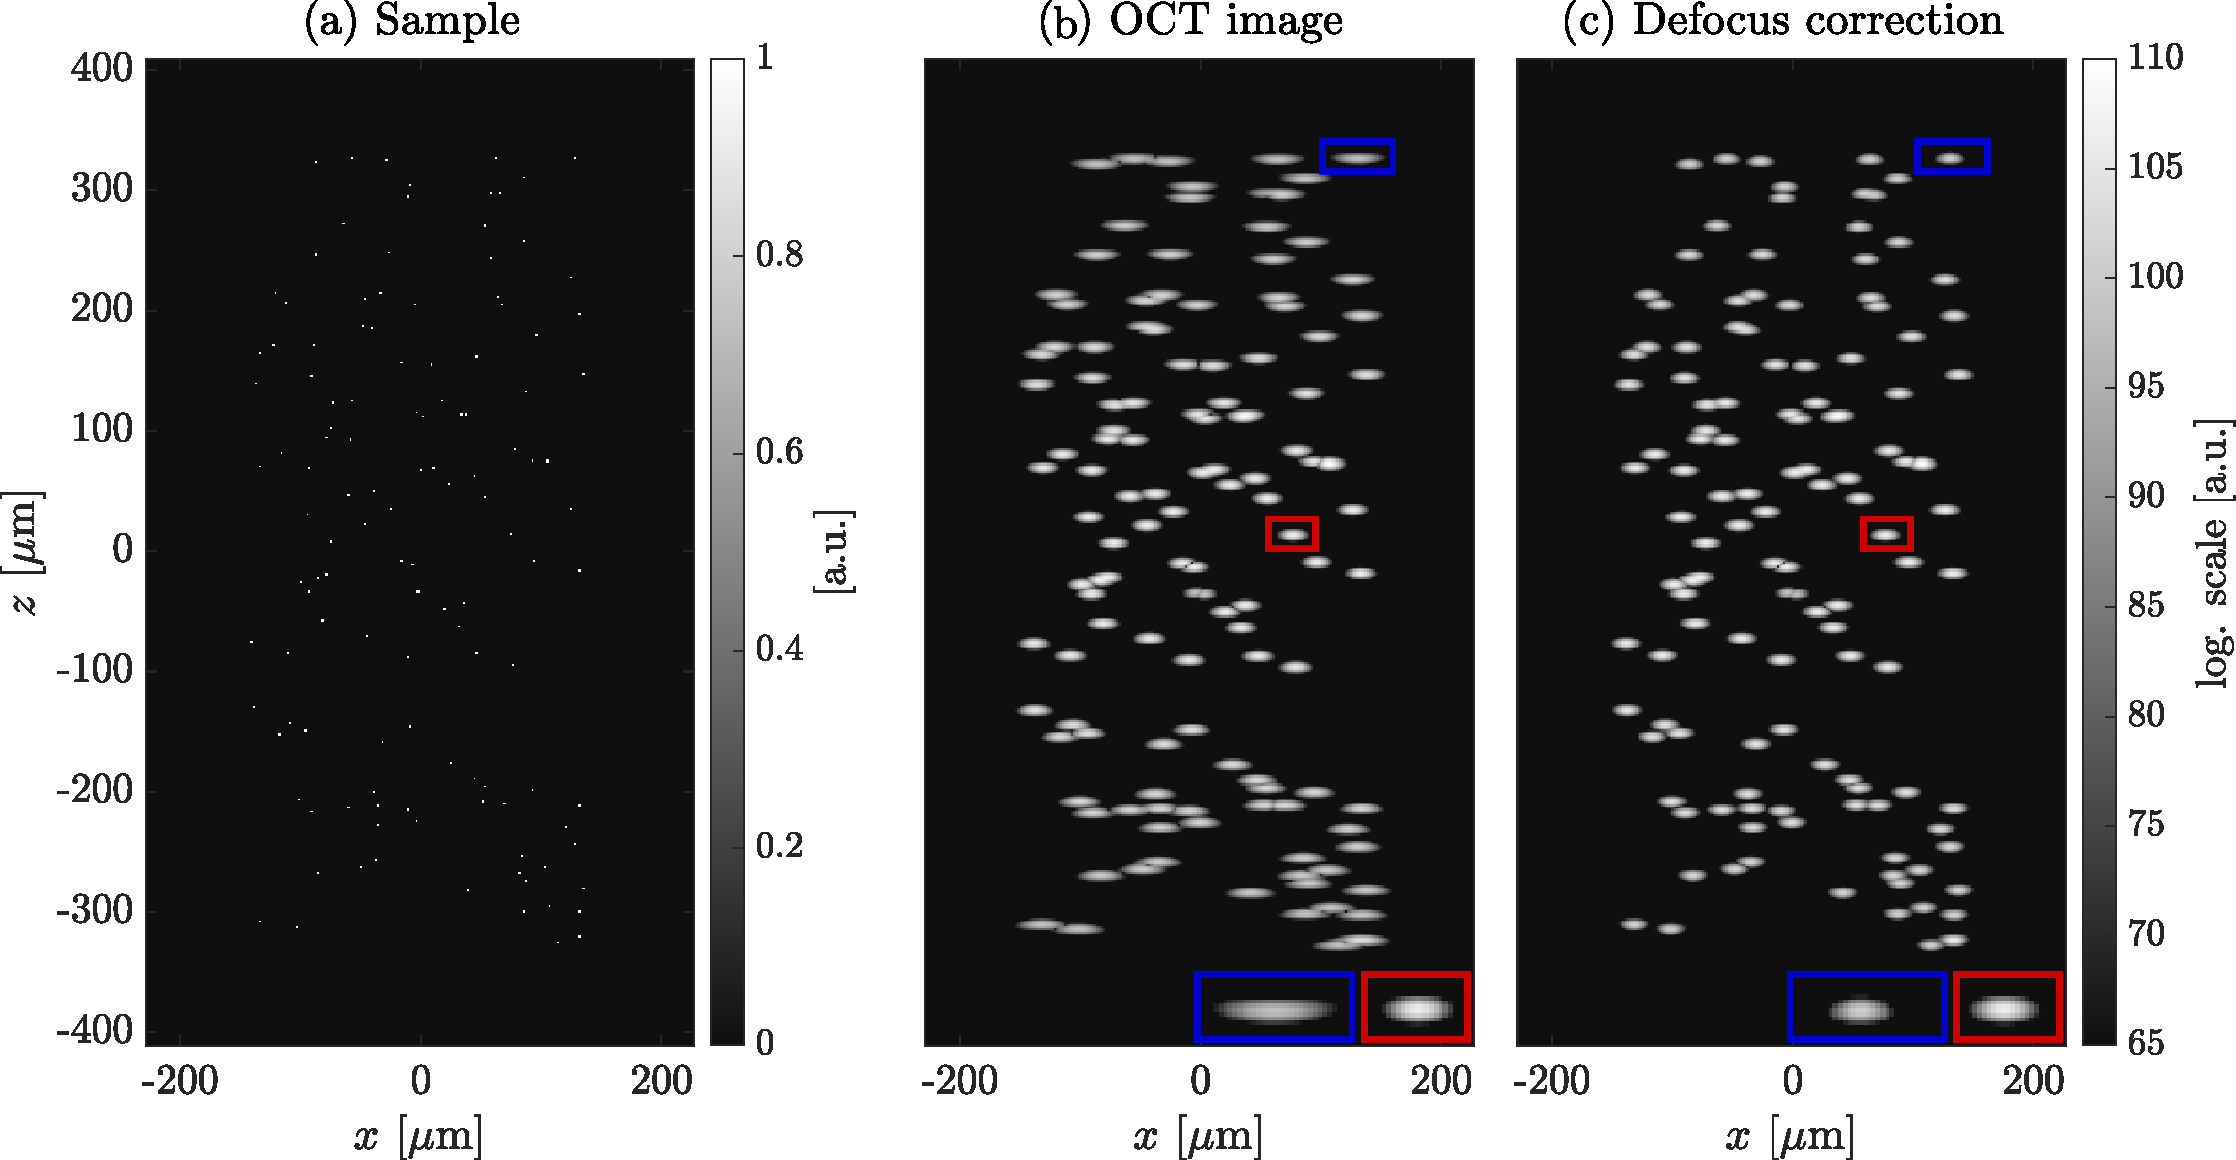
\includegraphics[width=\textwidth]{Figures/TheoreticalBasis/IM_Refocus.pdf}
    \caption[Illustration of digital refocusing.]{Illustration of digital refocusing. (a) Sample consisting of randomly located point scatterers, (b) OCT image simulated using the forward model, (c) Digital refocused. (b) and (c) are displayed in logarithmic scale.}
    \label{fig:IM2}
\end{figure}

\subsection{Computational adaptive optics}\label{sec:CAO}

Aberrations are wavefront distortions with respect to a reference wavefront, affecting image quality in imaging techniques such as OCT~\cite{Pircher2017_Review}. Several applications in OCT have benefited from aberration correction, whether using specific optical systems~\cite{Meemon2008_Optical, Xi2009_Highresolution,Mo2013_FocusExtension, Bo2017_Depthoffocus}, hardware-based adaptive optics~\cite{Zawadzki2005_Adaptiveoptics, Zhang2006_Highspeed} or computational adaptive optics~\cite{Kumar2017_Invivo, Hillmann2016_Aberrationfree, Fechtig2014_Line, Wu2019_Computed}. For instance, in retinal imaging, the probe beam is focused onto the retina using the optical system of the eye itself (cornea/lens) that may produce an distorted wavefront affecting image quality~\cite{Liang1997_Aberrations}. In particular, the wavefront in high NA systems is more susceptible to be distorted by imperfections of the optical systems or even the sample itself.

Defocus introduced in the propagation of light is intrinsic to the Gaussian probe beam, for this reason, it is not considered as an optical aberration, in this case aberrations are wavefront deviations from the ideal wavefront of a Gaussian beam. This can be noted in Eq.\eqref{eq:FMft}, where defocus arises from the exponential term whereas wavefront distortions can be modelled by $H(q_x, q_y; k)$ that is related to the effective generalized pupil of the optical system~\cite{Liu2017_Computational}, resulting from the convolution of the illumination and detection generalized pupils, that are identical in OCT given the double-pass geometry.

Recalling the forward model in frequency domain, it is possible to invert Eq.\eqref{eq:preISAM} to obtain an aberration-corrected OCT signal as
\begin{equation}\label{eq:preCAO}
    \tildehat{S}(q_x, q_y; k) = H^{-1}(q_x, q_y; k) \hat{S}(q_x, q_y; k).
\end{equation}
where $H^{-1}(q_x, q_y; k)$ acts as a frequency filter, which depends on spatial frequency and spectral domains, therefore it can address chromatic aberrations~\cite{Liu2017_Computational}. Given the relatively narrow spectrum of the light sources used in OCT, in practical scenarios it is convenient to assume a $k$-independent filter $H(q_x,q_y)$, which is the same for all depths~\cite{Liu2017_Computational}. In hardware adaptive optics (HAO), the correction filter $H^{-1}(q_x,q_y)$ is applied directly in situ to compensate for the distortions of the Gaussian beam~\cite{Zawadzki2005_Adaptiveoptics}, but, because coordinate re-sampling is not included in this expression, $\tilde{S}(q_x, q_y; k)$ is an aberration-corrected signal rather than the sample scattering potential, it means that defocus will be present yet in the acquired images. To correct for defocus using HAO, a depth-dependent phase filter is necessary but it is not possible with current hardware such as deformable mirrors. In the case of Computational adaptive optics (CAO), the filter is applied in post-processing~\cite{Adie2012_Computational}, enabling the combination of CAO with ISAM or digital refocusing to obtain aberration-free images with focal resolution throughout all depths, namely $\tilde{\eta}(x, y, z)$~\cite{Adie2012_Broadband}. In ISAM reconstruction $H^{-1}(q_x, q_y; k)$ is already included in Eq.\eqref{eq:ISAM}, note that  $\tildehat{S}(q_x, q_y; k)$ is written explicit in Eq.\eqref{eq:ISAM}. For low-NA regime, the depth-invariant filter $H(q_x,q_y)$ can be generalized in Eq.\eqref{eq:refocus} to a depth-dependent filter $H(q_x,q_y; z_d)$ that includes the exponential term, resulting in~\cite{Adie2012_Computational, Liu2017_Computational} 
\begin{equation}\label{eq:CAO}
    \tilde{\eta}(x, y; z) = \text{FT}_{q_x,q_y}^{-1}\left\{H^{-1}(q_x, q_y; z) \hat{S}(q_x, q_y; z)\right\}.
\end{equation}

In this case, defocus in treated as an aberration contained in the correction filter. $H^{-1}(q_x, q_y; z) = \Omega(q_x,q_z;z) e^{-i\varphi(q_x, q_y; z)}$ is a complex filter comprising an amplitude factor $\Omega(q_x,q_z;z)$ and a phase factor $e^{-i\varphi(q_x, q_y; z)}$. Phase factor is explicit in Eq.\eqref{eq:refocus} as $e^{iz_dq^2/4k_c}$ but the idea of CAO is to adaptively defined the phase factor based on the data rather than using the analytical expression~\cite{Adie2012_Computational}, which only accounts for defocus and requires precise knowledge of physical quantities of the system, for instance, the location of the focal plane in the tomogram. The procedure to obtain an aberration-correction sample scattering potential using Eq.\eqref{eq:CAO} is rather simple (note that it is a spatial deconvolution performed in Fourier domain) the key point is to determine the appropriate correction filter. In CAO, the amplitude factor $\Omega(q_x,q_z;z)$ is usually set to unity, because it does not produce a significant impact in image distortions, and a phase-only filter $H(q_x,q_y)=e^{-i\tilde{\varphi}(q_x, q_y; z)}$ is used, where the approximate phase $\tilde{\varphi}(q_x, q_y; z)$ is described in terms of a polynomial basis, such as Zernike polynomials $Z_i$ which are a convention for the description of optical aberrations~\cite{Malacara2007_Optical, Lakshminarayanan2011_Zernike}. Using a weighted sum with $N$ Zernike polynomials, $\tilde{\varphi}(q_x, q_y; z)$ is expressed as
\begin{equation}\label{eq:PhaseDecomp}
	\tilde{\varphi}(q_x, q_y; z) = \sum_i^N Z_i\alpha_i(z_d),
\end{equation} 
with weights $\alpha_i(z)$ that vary with depth. To determine $\alpha_i(z)$, there are two general approaches, optimization-based~\cite{Adie2012_Computational} and sub-apertures correlation~\cite{Kumar2013_Subaperture}.

Sub-apertures correlation method proposed by Kumar et al. consists in measuring the local slope of the wavefront in the pupil/Fourier plane to determine the correction phase, emulating a Shack-Hartmann sensor~\cite{Kumar2013_Subaperture}. To do so, the Fourier transform of the acquire signal for each depth, namely $\hat{S}(q_x, q_y; z)$, is split into sub-apertures and the inverse Fourier transform of each sub-aperture is computed to yield images that will exhibit lower resolution and relative shifts between them. These image are cross-correlated to the image of a reference sub-aperture to measure the relative shifts, that is related to the local slope of the wavefront. Then, the local slopes are used to construct the phase correction, possibly using a decomposition like Eq.\eqref{eq:PhaseDecomp}. The number of sub-apertures determines the degree of aberrations that can be corrected. For instance, splitting the pupil into two vertical and horizontal apertures enables defocus correction along the two scan axis. A large number of sub-apertures is desired to be able to correct for high-order aberrations, however, this leads to a significant resolution loss and increased image correlation error, which ultimately results in high errors in the determination of the correction phase.

Optimization-based CAO proposed by Addie et al.~\cite{Adie2012_Computational} consists in finding the set of weights $\alpha_i(z_d)$ that improves image quality as measured by a metric via optimization. The iterative operation of this procedure may increase computational time compared to sub-aperture based CAO, but it allows to straightforwardly include high-order aberrations by increasing the number of polynomials and weights used in the correction phase composition. Optimization-based CAO relies on the definition of a proper image quality metric, that ideally must have a minimum (or a maximum) when image aberrations are well compensated, being image sharpness metrics most used for this purpose since aberrations correction is supposed to improve sharpness.

Shannon's entropy metric $\text{SE}(I)$ of an image $I_{m,n}$ with discrete indexes $(m,n)$ and size $M\times N$ is known to be minimal when aberrations are minimized, it has been used in the context of CAO in OCT~\cite{Hillmann2016_Aberrationfree}, brought from SAR imaging~\cite{Flores1992_Robust}, and is given by
\begin{equation}\label{eq:SE}
	\text{SE}(I) = \sum_i^M\sum_j^N \Gamma(\bar{I}_{i,j}),
\end{equation}
where $\Gamma(I) = -I\log I$, although different transformations can be used, and
\begin{equation}
	\bar{I} = \left|\frac{I}{\sum_i^M\sum_j^N \left|I_{i,j}\right|}\right|^2
\end{equation}
is a normalized intensity image. Here, $I_{m.n}=S_{m,n,l}$ is the current $l$-th \textit{en face} plane being compensated [recall that $S_{m,n,l}$ refers to the discrete version of $S(x,y,z)$].

There are several image quality metrics that have been used in the context of other imaging modalities such as digital holography~\cite{Trujillo2015_Comparative}. For instance, Tamura's coefficient $T = \sqrt{\frac{\sigma(I)}{\left<I\right>}}$ is a measure of contrast~\cite{Memmolo2011_Automatic}, where $\sigma(\cdot)$ is the standard deviation and $\left<\cdot\right>$ is the average value, and gradient-based metrics such as
\begin{equation}
	\text{G(I)} = \sum_i^M\sum_j^N \sqrt{\left[I_{i,j}-I_{i-1,j}\right] ^2 + \left[I_{i,j}-I_{i,j-1}\right] ^2}
\end{equation}
where $I_{m,n} = |S_{m,n,l}| ^ 2$. Image spatial frequency content metrics have been used in sensor-less HAO and eventually in CAO~\cite{Debarre2007_Image}, and are based on the fact that mid- to high-frequency content of the complex amplitude should increase as resolution improves, i.e. when aberrations are minimized. One possible estimation is the ratio of energy within a band-pass frequency range to the total energy~\cite{Adie2012_Computational}, expressed as
\begin{equation}
	\text{F}(I) = \frac{\sum_i^M\sum_j^N |I_{i,j}B_{i,j}|^2 }{\sum_i^M\sum_j^N |I_{i,j}|^2}
\end{equation}
where $I_{m,n} = \hat{S}_{q_m, q_n,l}$, being $(q_m, q_n)$ discrete counterparts of $(q_x, q_y)$, and $B_{m,n}$ is a band-pass filter with cut-off frequencies tuned to obtain a good performance.

Figure~\ref{fig:CAO} illustrates the effect of aberrations in a simulated \textit{en face} ($xy$ plane) OCT image that was generated elsewhere~\cite{Cuartas-Velez2017_Formacion} with a probe beam waist diameter of $10~\mu$m. The tomogram consists of a large number of point scatterers distributed in the entire field of view as occurs in tissues, with similar index of refraction, producing speckle. In addition, point scatterers with a different index of refraction were added and arranged in a cylindrical shape along horizontal axis $x$, appearing as bright rectangles in the cross-sectional \textit{en face} view of Fig.\ref{fig:CAO}(a) located at the focal plane. Eq.\eqref{eq:defocus} was used to induce defocus as if the \textit{en face} plane of Fig.\ref{fig:CAO}(a) were located at $z=200~\mu$m from the focal plane, and defining the phase of $H$ shown in Fig.\ref{fig:CAO}(e), using Zernike polynomials $Z_5$ and $Z_7$ to induced astigmatism and coma aberrations with random magnitudes, resulting in the aberrated \textit{en face} of Fig.\ref{fig:CAO}(b), where blurring is evident and consequently resolution loss.

Digital refocusing was applied to the aberrated \textit{en face} using Eq.\eqref{eq:refocus} setting $H=1$, resulting in a refocused image with partial resolution improvement due to the presence of the remaining two aberrations deteriorating image quality. On the other hand, optimization-based CAO was applied to the aberrated \textit{en face} using Eq.\eqref{eq:CAO}, describing the phase correction filter with $Z_4$, $Z_5$ and $Z_7$, being $Z_4$ Zernike polynomial for defocus. Aberration-corrected \textit{en face} view of Fig.\ref{fig:CAO}(d) exhibits focal resolution similar to the original \textit{en face}, demonstrating the possibility of correcting defocus and additional aberrations using CAO.
 
\begin{figure}[htb!]
	\centering
	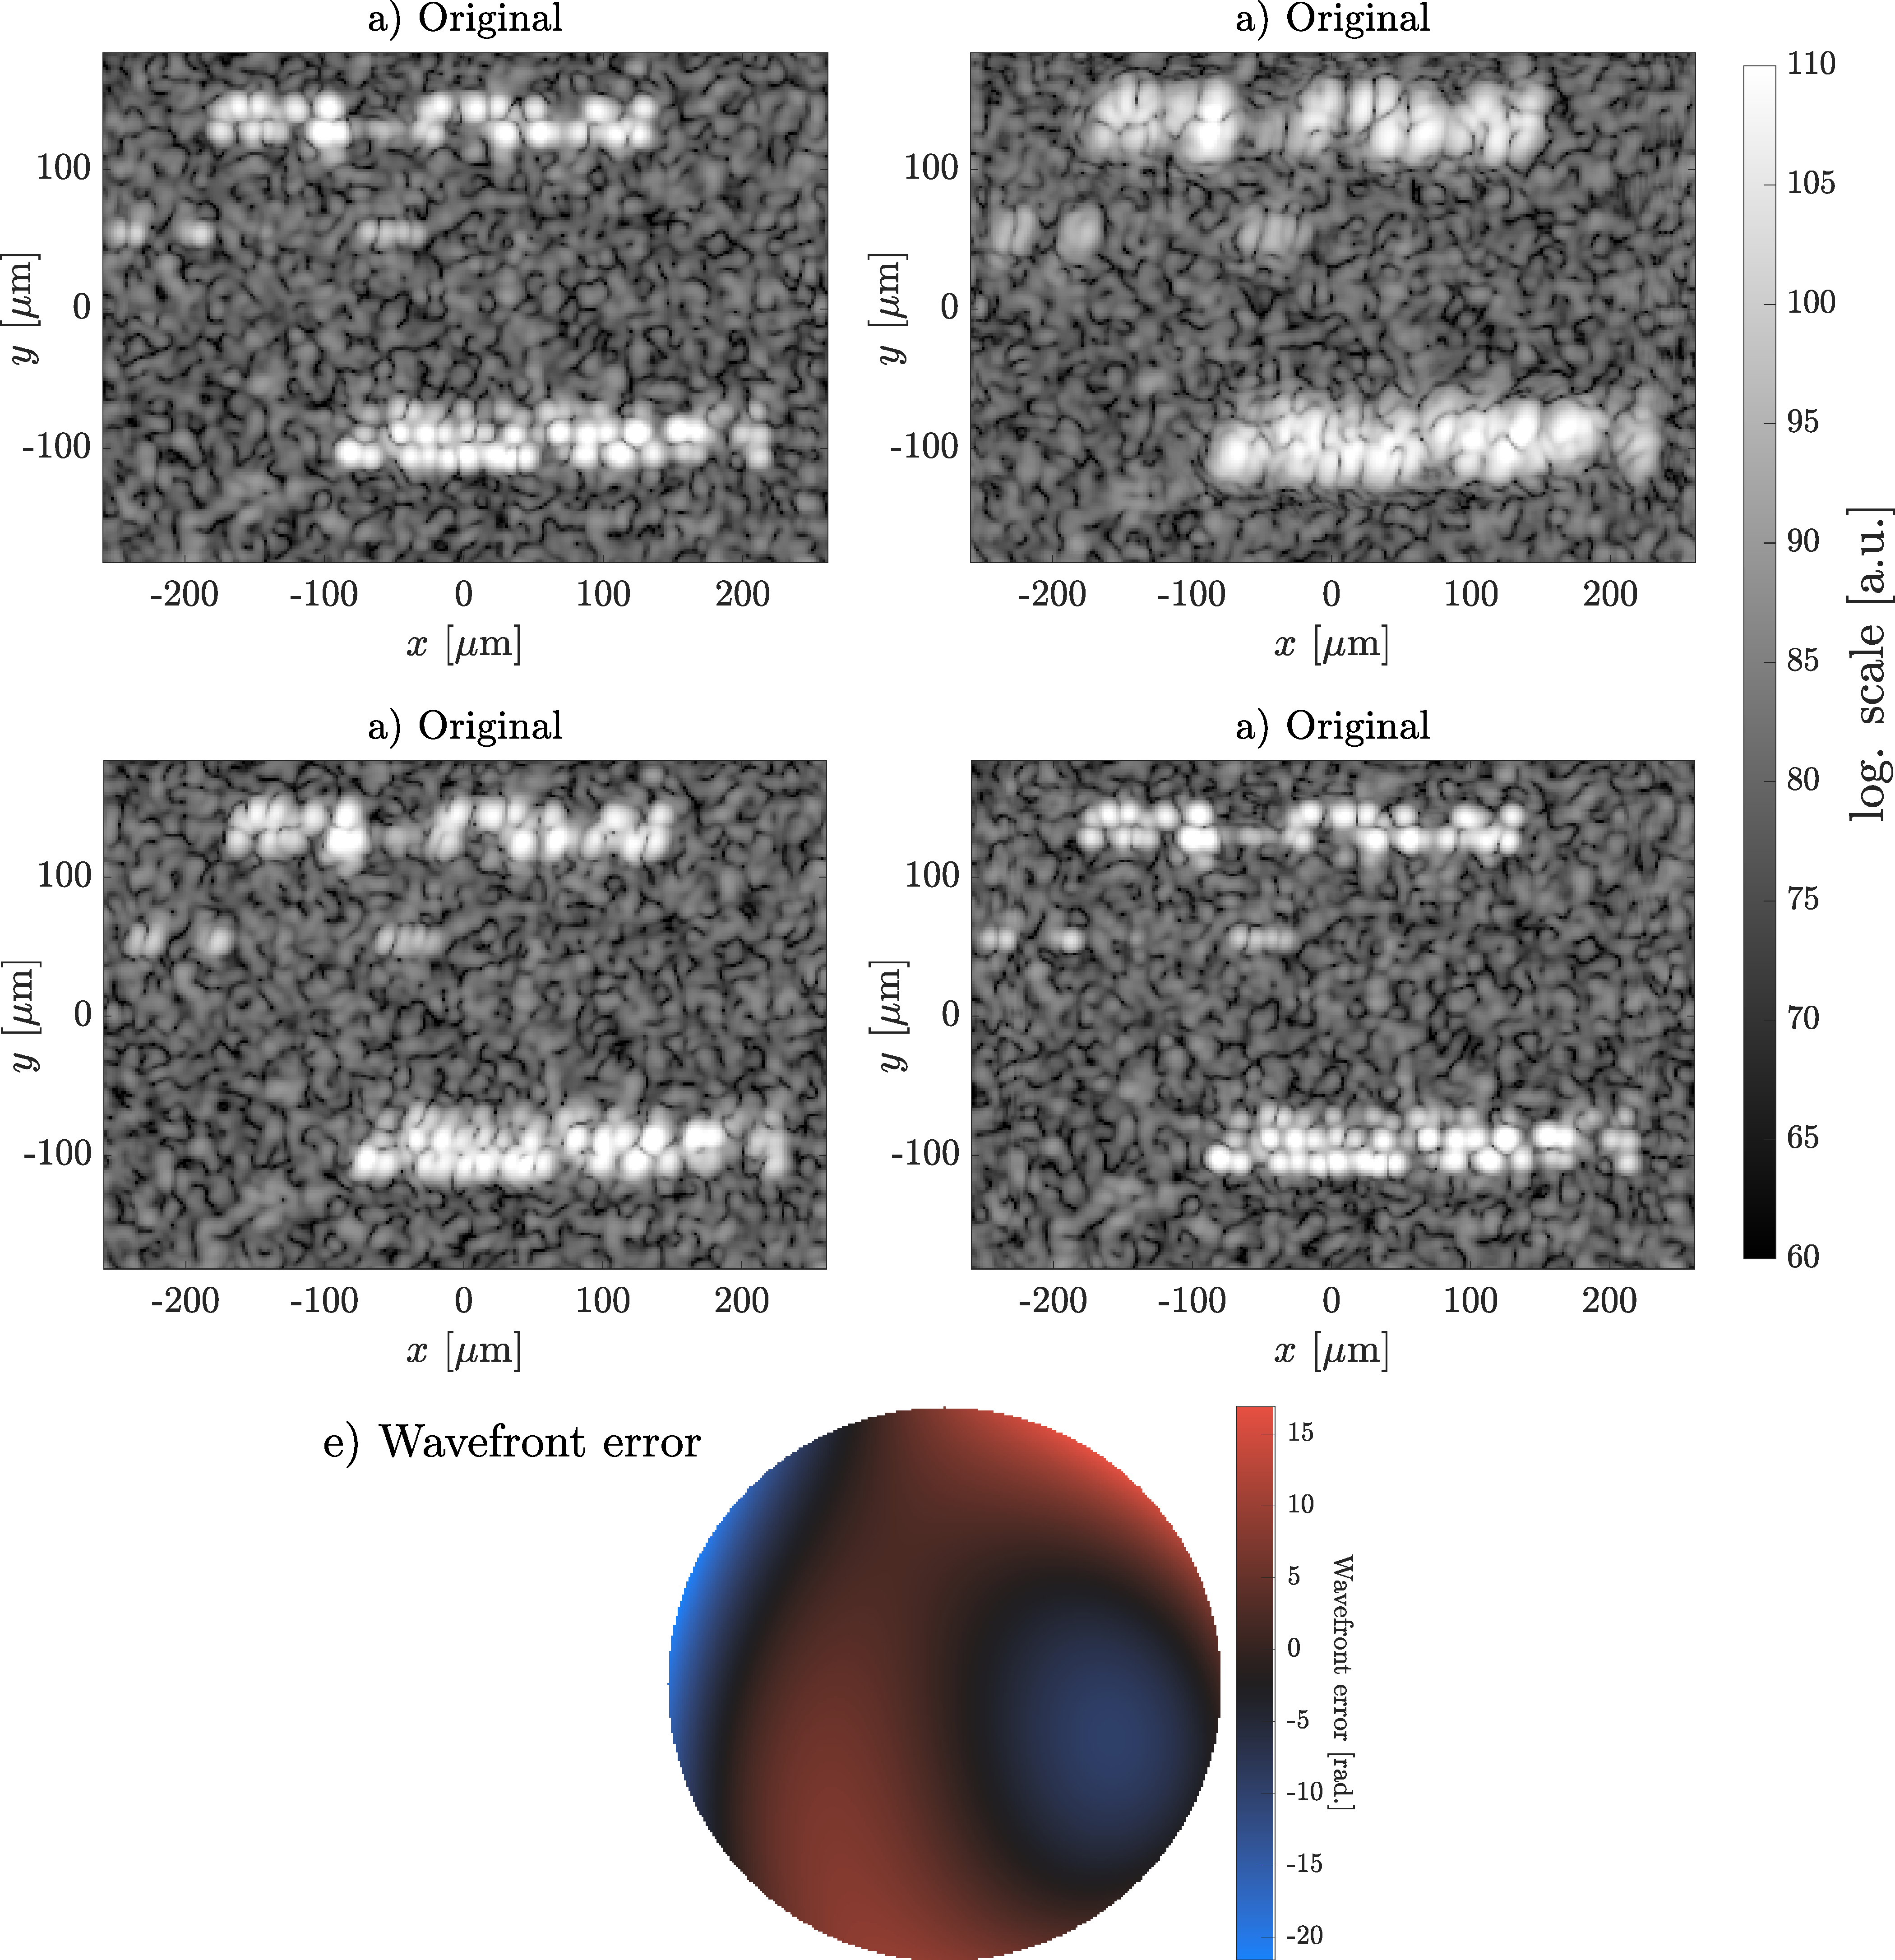
\includegraphics[width=\textwidth]{Figures/TheoreticalBasis/CAO.pdf}
	\caption[Illustration of computational adaptive optics.]{Illustration of computational adaptive optics. Simulated OCT \textit{en face} image (a) without and (b) with aberrations and defocus, induced using the wavefront in (e). Result of (c) digital refocusing and (d) computational adaptive optics. (a)--(d) are displayed in logarithm scale.}
	\label{fig:CAO}
\end{figure}

To illustrate the behavior of image quality metric that is the basis of CAO, original \textit{en face} of Fig.\ref{fig:CAO}(a) was defocused using $Z_4$ weighted by $\alpha_4=17.8$ and then several corrected images were created with weights linearly varying between $[-40, 20]$. Figure~\ref{fig:Sharpness} shows a plot of Shannon's entropy of the corrected image as a function of the correction weight $\tilde{\alpha}_4$, exhibiting a smooth behavior with a clear minimum at nearly $\tilde{\alpha}_4=-17.8$, where the negative sign is because the correction phase term is the conjugate of the applied defocus term. Alongside Shannong's Entropy, there are six example \textit{en faces} with different phase corrections, with the optimal \textit{en face} enclosed in a red box, showing the best image quality among them.

\begin{figure}[htb!]
	\centering
	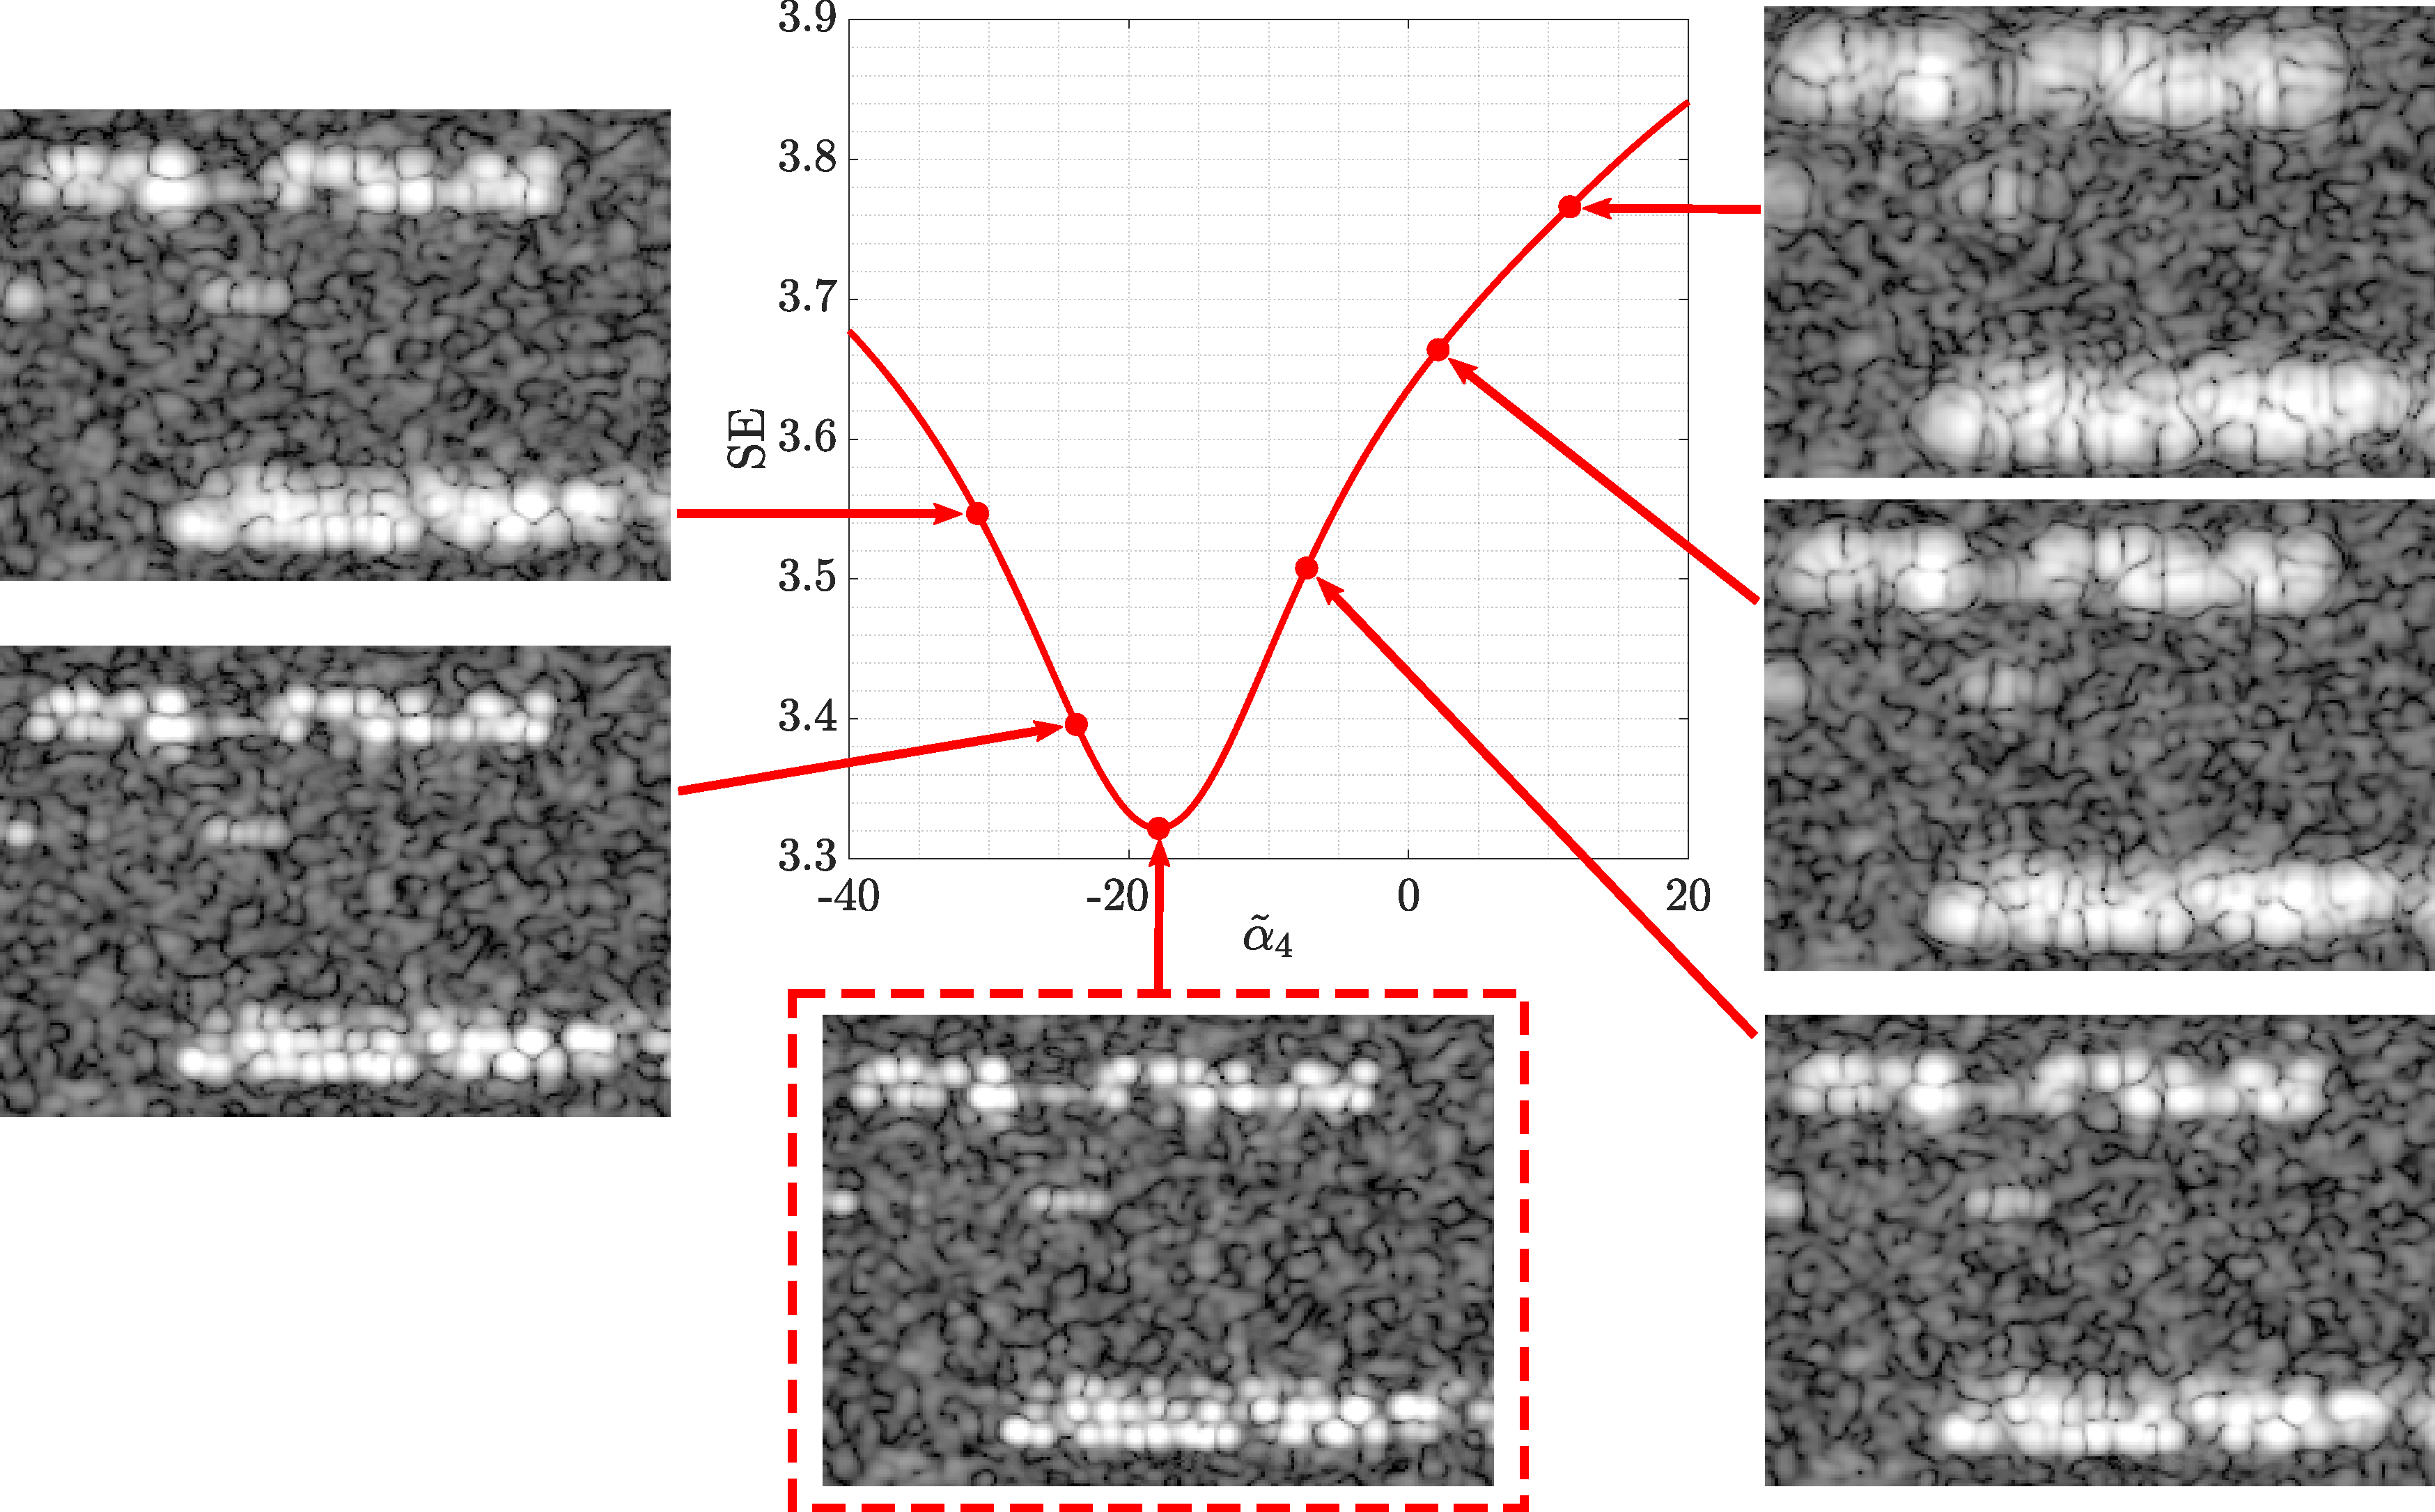
\includegraphics[width=\textwidth]{Figures/TheoreticalBasis/SharpnessCAO.pdf}
	\caption[Illustration of Shannon's entropy metric.]{Illustration of Shannon's entropy metric to measure image sharpness of a defocused \textit{en face} image corrected using Zernike polynomial $Z_4$. Plot shows the value of SE as a function of correction weight $\tilde{\alpha}_4$. Surrounding \textit{en faces} images were corrected with different weights for a visual inspection of image quality. Optimal corrected image (on the red rectangle) corresponds to the minimum value of SE.}
	\label{fig:Sharpness}
\end{figure}

Computational adaptive optics promises to be a powerful alternative to hardware-based adaptive optics that require very complex optical setups, specially in retinal imaging where the demand of cellular imaging increases, for example in photo-receptors mosaic imaging~\cite{Kumar2017_Invivo, Hillmann2016_Aberrationfree, South2018_Combined}.

There are two necessary requirements for computational aberration correction. Acquired tomogram should possess phase stability which is so far the major requirement~\cite{Shemonski2014_Stability, Liu2017_Computational, South2016_Computed}, but in addition the lateral sampling must satisfy Nyquist sampling~\cite{Liu2017_Computational}, i.e. lateral sampling must be equal or smaller than half the beam waist diameter, otherwise high-frequency content is not recovered properly and results will present distortions. In fact, Nyquist sampling is necessary in general for computational refocusing in any imaging technique, not only in OCT~\cite{Wallace2001_Workingpersons, Pawley2006_Handbook, Biggs2010_3D}. 

\subsection{Phase stability requirement} \label{sec:phaseStab}

Computational techniques described previously rely upon accurate measurements of the complex amplitude information in order to guarantee a coherent aperture synthesis, necessary for aberration correction. Complex amplitude comprises amplitude and phase information, but phase is more susceptible to undesired fluctuations~\cite{Vakoc2005_Phaseresolved}, hence reliable phase measurement is not a straightforward task due to experimental contains as explained in Section~\ref{sec:OCTConfigPhaseStab}. In fact, first digital refocusing approaches in OCT were based on the intensity~\cite{Ralston2005_Deconvolution, Woolliams2010_Spatially, Y.Liu2009_Deconvolution}, but they provide very limited results given that incoherent deconvolution ignores the phase information. Such initial approaches were designed to work with the intensity signal possibly because the lack of phase stable measurements in early OCT systems.

The aim of this section is to discus phase stability requirement in the context of computational aberration correction. Phase stability is affected by phase noise that may arise from the system or the sample. System-induced phase noises, such as phase-jitter~\cite{Vakoc2005_Phaseresolved} and galvanometer-induced phase noise~\cite{Adie2015_Interferometric, White2003_vivo}, were explained in Section~\ref{sec:OCTConfigPhaseStab}. On the other hand, sample-induced phase noise arises from sample motion~\cite{Shemonski2014_Stability-1}, therefore it affects mainly \textit{in vivo} imaging which is more prone to motion during signal acquisition than \textit{ex vivo} imaging, either global motion, such as involutary motion of the subject, or internal such as blood flow in arteries.

Development of computational aberration correction has been grounded in SDOCT systems. For this reason, most significant phase instabilities induced by the system arise from the galvanometer scanners, which can be experimentally avoided in some cases, therefore, in this area, major attention have been put in sample motion-induced phase noise, which is the focus of following discussions.

Sample motion have two primary effects in the complex OCT signal; effective shift of the complex amplitude and phase-only jump~\cite{Chen1997_Optical, White2003_vivo, Shemonski2014_Stability}. The former effect is rather intuitive, it is the displacement of apparent location of the signal in the tomogram, affecting both amplitude and phase. The latter effect is an additional phase-only jump that is a consequence of Doppler effect, and actually it is used for functional imaging techniques like flowmetry~\cite{Braaf2019_OCTBased}. Both effects have an impact in the phase of the tomogram and therefore they affect phase stability, but their individual influence vary depending on system parameters~\cite{Shemonski2014_Stability}. Effective complex amplitude shift scales with the spatial resolution of the system; the higher the resolution, the more susceptible the system may be to motion. In general, axial resolution is finer than lateral resolution, therefore this effect have a greater impact in the axial direction. On the other hand, phase-only jump $\delta$ is a consequence of motion in the axial direction only, and is proportional to the axial displacement $\delta z$ and the central wavenumber, $\delta = 2k_c\delta z$, where the factor of two is due to the double-pass, reflection geometry. Since $k$ is typically a relatively large value (of the order of $10^6$) relatively small displacements $\delta z$ can produce significant phase jumps $\delta$, and this is why optical phase-sensitive techniques can measure very small displacement using optical interferometry, but in the case of CAC this is an undesired phase contribution that in general have a greater influence than complex amplitude shift effect. For this reason, in some cases there is not an evident displacement in the tomogram intensity due to motion, yet there may be phase jumps reducing phase stability.

In practical terms, motion artifacts are negligible during one A-line acquisition under controlled circumstances, in the case of SDOCT because the parallel acquisition in $k$-space, and in SSOCT because the high A-line acquisition rate. However, motion artifacts may appear during acquisition of multiple A-lines and more significantly during acquisition of multiple B-scans which have a longer repetition time. Complex amplitude shifts appear as relative displacements between A-lines or B-scans, whereas phase-only jumps produce a relative phase offset between A-lines or B-scans. For these reasons, hereafter 1D and 2D phase stability are used to refer to phase stability along one or two lateral scan axes, obviating phase stability along axal direction which in general is ensured.

Figure~\ref{fig:motionEx} illustrates the effect of motion artifacts in OCT images and phase stability, using a simulated B-scan generated similarly to that of Fig.\ref{fig:IM2}, except that axial motion was added when computing the $n$-th A-line by changing the position $z$ of all scatters by $z + \delta z_n$, where $\delta z_n$ represents the magnitude of motion, with random values inside a predefined range for every A-line. This corresponds to a rigid body or \textit{bulk} motion because the entire sample is displaced by the same amount in every A-line. The simulated intensity B-scan with a static sample is shown in Fig.\ref{fig:motionEx}(a), displaying defocus away from the focal plane located at $z=0$. This image was re-generated inducing inter-A-line motion randomly distributed with standard deviation $1~\mu$m, shown in Fig.\ref{fig:motionEx}(d), and the resulting intensity B-scan shown in Fig.\ref{fig:motionEx}(b) exhibits spurious relative shifts between A-lines, which in this case are evident because the magnitude of motion is of the order of axial resolution 5~$\mu$m.

\begin{figure}[]
	\centering
	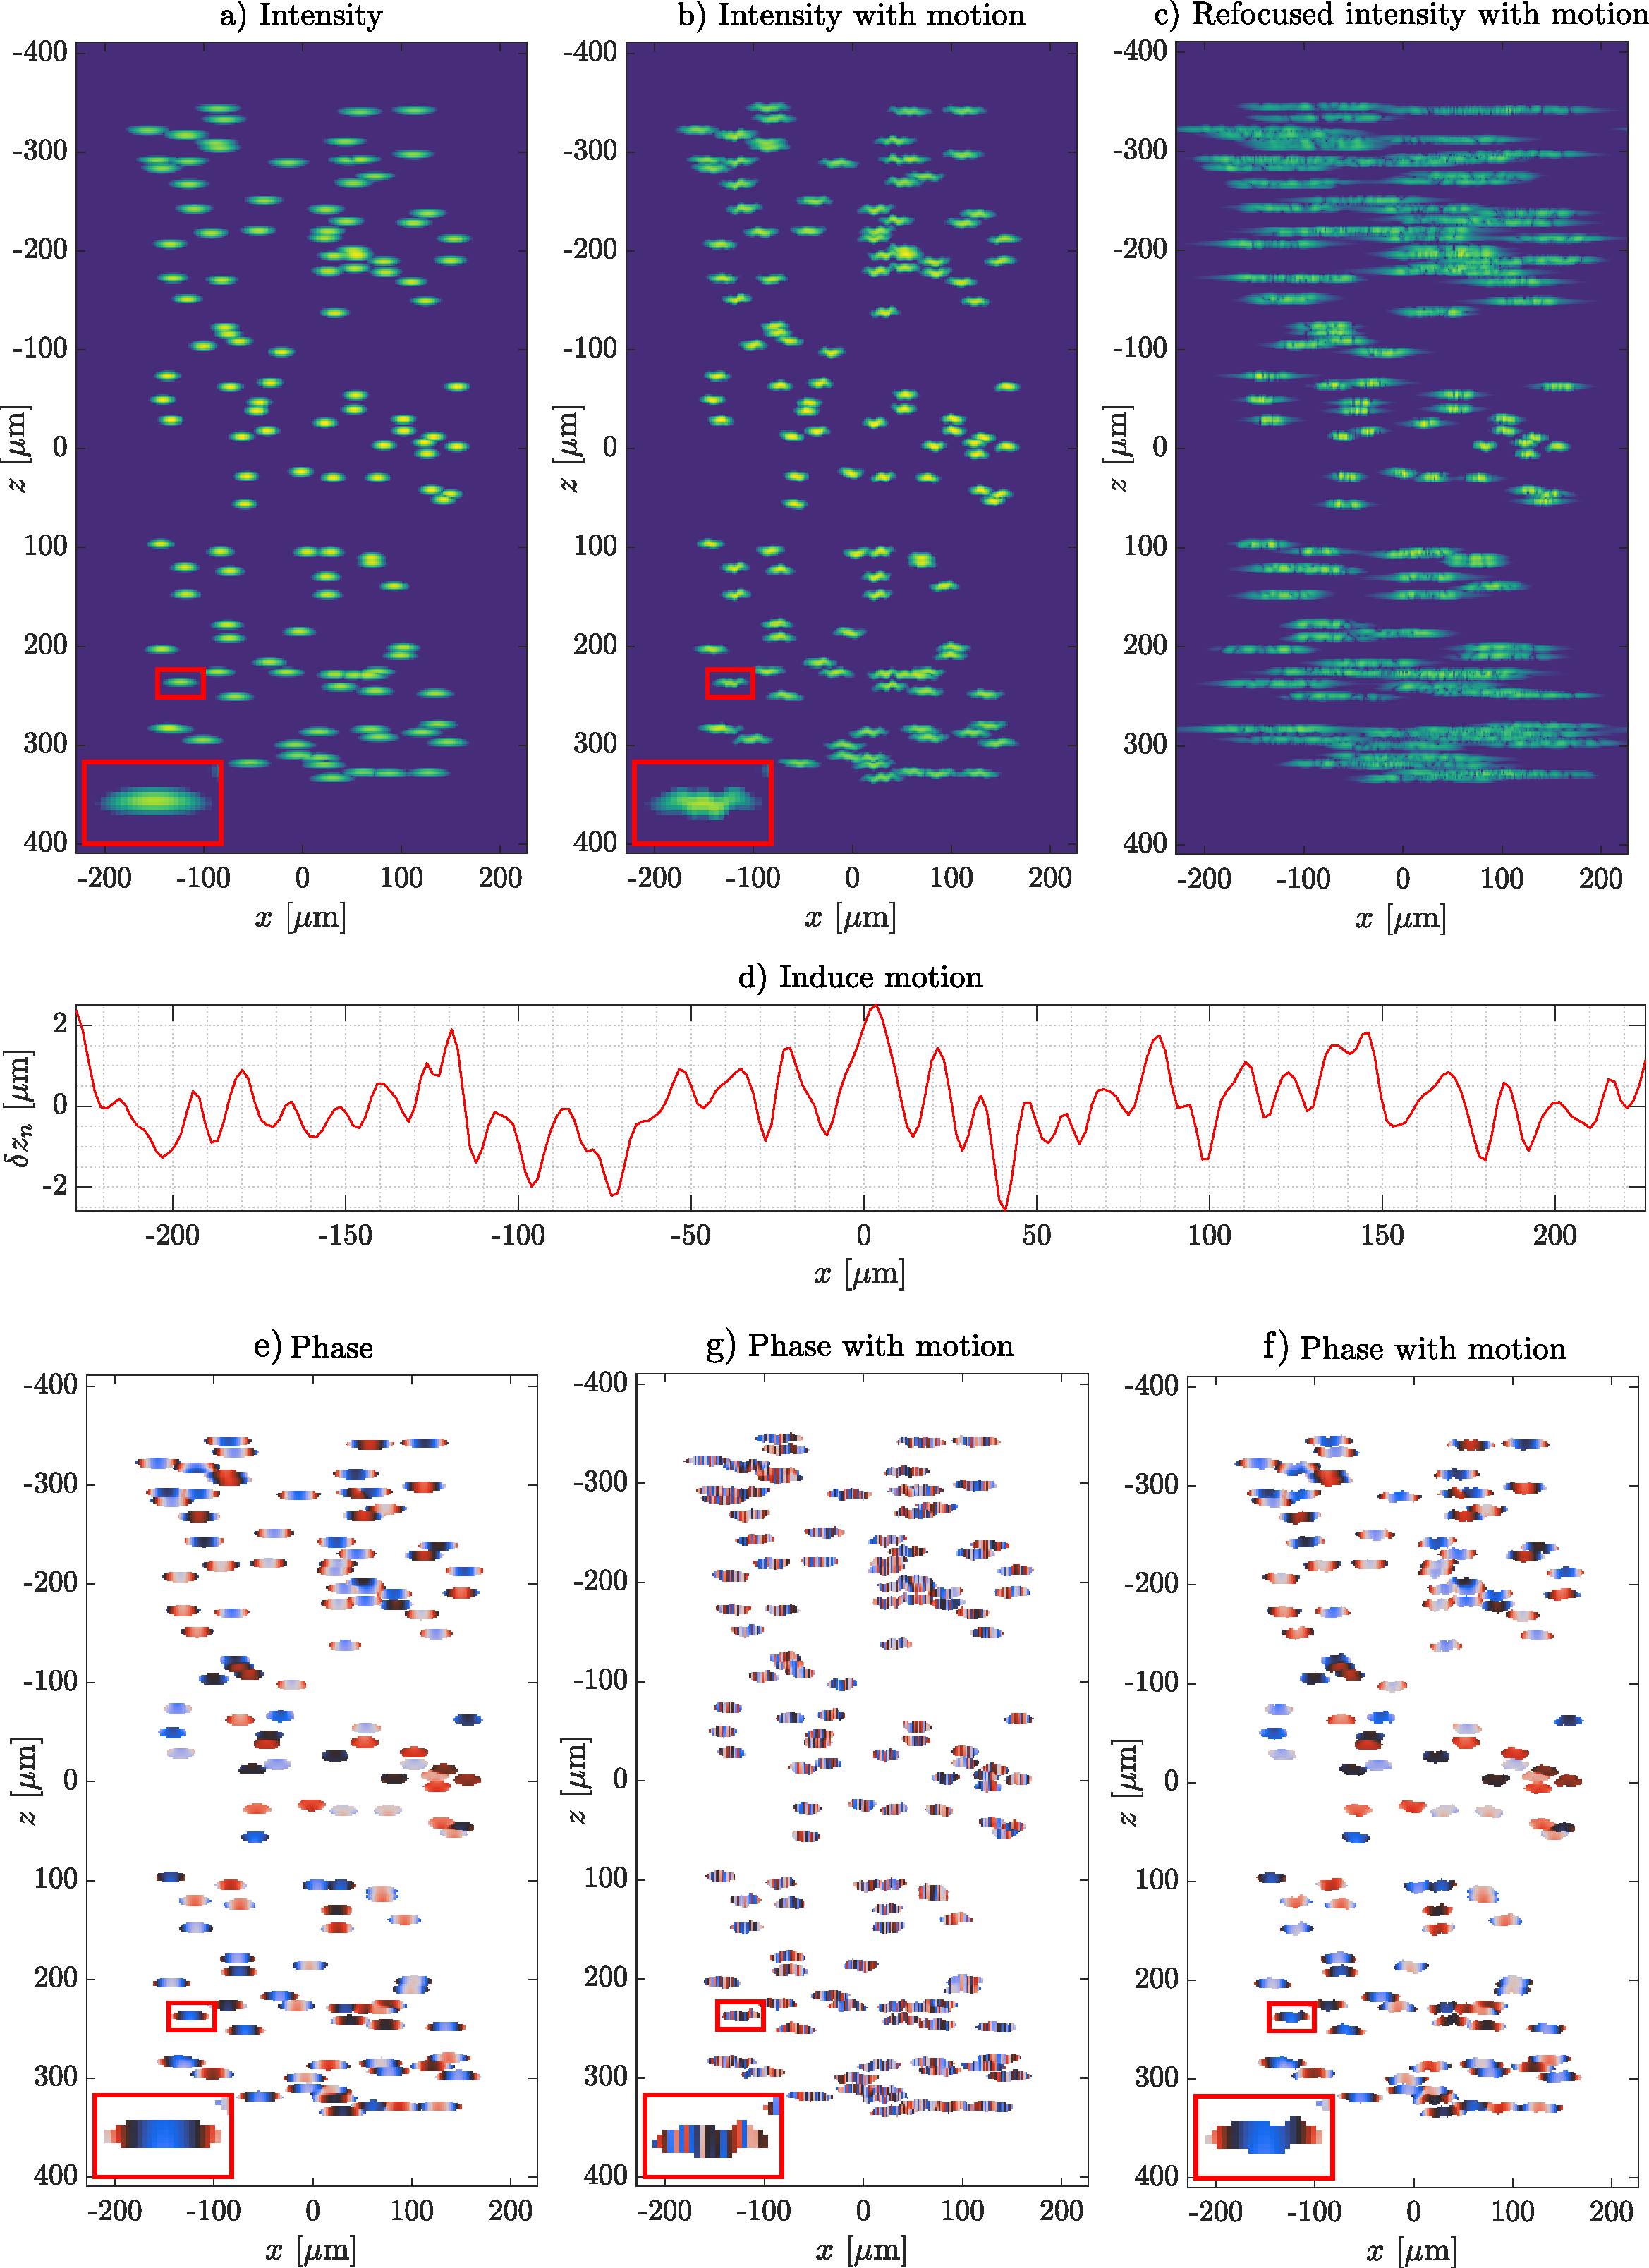
\includegraphics[width=.95\textwidth]{Figures/TheoreticalBasis/MotionEx.pdf}
	\caption[Illustration of the impact of motion in phase stability and digital refocusing.]{Illustration of the impact of motion in phase stability and digital refocusing. OCT image simulated using the forward model, (a) with static sample; (b) with sample motion shown in (d), that results in the unsuccessful digital refocused image (c) refocusing. Note the relative shift between A-lines when comparing the insets in red rectangles. Phase image: (a) with static sample; (g) with sample motion shown in (d) and the same of (g) but ignoring the phase-only jumps.}
	\label{fig:motionEx}
\end{figure}

To evaluate phase stability, Fig.\ref{fig:motionEx} shows phase images computed as $\arg\{S_{m,n,l}\}$, where a threshold was used to display only regions with high intensity, corresponding to the point scatterers. Fig.\ref{fig:motionEx}(e) is the phase with the static sample, exhibiting a stochastic but smooth behavior, distinctive of phase stable images, opposed to the phase image after inducing motion shown in Fig.\ref{fig:motionEx}(e) that exhibits very poor phase stability because of the relative shifts between A-lines, also observable in the intensity image in Fig.\ref{fig:motionEx}(b), and more importantly due to the random phase offsets induced by Doppler jumps, not observable in the intensity image in Fig.\ref{fig:motionEx}(b). Lack of phase stability frustrates the operation of digital refocusing or any other phase-dependent aberration correction method, as is evident in Fig.\ref{fig:motionEx}(c). To compare the influence of the two effects of motion, Fig.\ref{fig:motionEx}(f) shows the phase when ignoring the motion-induced phase offsets, thus considering only the complex amplitude shifts, and it can be noted that phase is smoother than that of Fig.\ref{fig:motionEx}(g) affected by both motion artifacts, however, even ignoring phase jumps, in this example complex amplitude shifts alone are strong enough to frustrate any aberration correction.

To quantitatively determine that certain tomogram has sufficient phase stability for a phase-dependent technique to work properly is somewhat not possible (unless attempts are performed to evaluate results), instead, it is possible to recognize when phase stability is not enough for such techniques to provide reliable results. Some systematic studies have been carried out to show the effect of various types of motion on defocus correction, namely, 1-D Brownian motion, steps functions and sinusoidal motion, and this helped to determined thresholds for admissible motion magnitudes for successful aberration correction to assist the design of OCT systems, for instance to determine an adequate imaging speed. Such works include simulated studies, as well as experimental studies with \textit{ex vivo} sample~\cite{Shemonski2014_Stability}, and a further extension with \textit{in vivo} imaging~\cite{Shemonski2014_Stability-1}, finding out that in terms of motion-induce phase noise, axial motion plays indeed the most important role in phase stability, although in some experimental scenarios traverse motion may be significant as well.

It is important to recall that phase stability is more difficult to achieve in SSOCT compared to SDOCT given that the former is susceptible to phase-jitter describing a linear depth-dependent noise, in addition to the phase noise sources affecting in SDOCT.

\subsection{Phase stabilization}\label{sec:phaseStabilization}

Given that the presence of phase noise in acquired tomograms is quite difficult to avoid or suppress experimentally~\cite{Adie2015_Interferometric}, phase stabilization in post-processing have been developed for phase-dependent imaging techniques in OCT like aberration correction and Doppler OCT. Phase stabilization techniques were designed to correct for phase jumps between A-lines, whether they arise from sample-motion or the system itself, but they cannot address complex amplitude shifts so that they must be small enough to be considered negligible. In this section, numerical phase stabilization approaches are presented oriented to the correction of phase offsets. In fact, correction of phase offsets is not sufficient for phase-jitter correction which is a linear depth-dependent phase noise, however the methods presented here can be extended to address phase-jitter with slight modification, and the core discussions of this section applies equally for this type of phase noise.

An early phase stabilization approach employs a reference signal consisting in an highly reflective flat surface in the sample arm, like a mirror or even a coverslip~\cite{Ralston2006_Phase, Yang2001_Phasereferenced}. The phase of this reference signal is assumed to be space-invariant, thereby any phase jump between A-lines must be due to phase noise. The procedure consist in identifying and extracting the reference signal in the tomogram $S(m,n,l)$, which should appear across the entire lateral field of view but typically occupy only a small set of pixels $L$ in the axial direction, and in a phase stable tomogram it should have a constant phase value. Then, the phase difference between adjacent A-lines $m$ and $m-1$ are computed as
\begin{equation}\label{eq:PhaseDiff}
	\delta(m,n) = \arg\left\{\sum_{l\in L} S(m,n,l)S^*(m-1,n,l)\right\},
\end{equation}
where $^*$ denotes complex conjugate and the summation over $L$ is to average the phase of phasors along depth. Phase differences $\delta(m,n)$ are relative to consecutive A-lines, the absolute phase differences $\Delta(m,n)$ with respect to a reference A-line, typically first A-line, are calculated using a cumulative sum as
\begin{equation} \label{eq:absPhaseDiff}
	\Delta(m,n) = \sum_{\hat{m}=1}^m \delta(\hat{m},n).
\end{equation}

Finally, the phase-corrected tomogram $\tilde{S}(m,n,l)$ is corrected applying the conjugate phase differences,
\begin{equation}
	\tilde{S}(m,n,l) = S(m,n,l)e^{-i\Delta(m,n)}
\end{equation}

To summarize, this phase stabilization process consist in applying a conjugate phase offset that is determined for each A-line using the phase difference between consecutive A-lines considering only a region of the signal containing a reference constant phase. There are some important features to remark. First, the correction phase is depth-independent; it consists of a global phase offset for every A-line, so that it cannot correct for phase-jitter which is a depth-dependent ramp phase noise as noted in Eq.\eqref{eq:phaseJitter}, an extension to cover phase-jitter is possible and has been developed~\cite{Vakoc2005_Phaseresolved} as will be explained later. Second, the need of a reflective surface in the sample arm is difficult to implement in practical terms, specially for \textit{in vivo} imaging where it is not easy to add a mirror in the sample arm directly. A very used approach is to separate the sample arm into two paths, one for the sample and the other for a mirror, but this is based on hardware modifications not present in basic OCT setups. 

This hardware-based phase stabilization approach was crucial for the development of CAC techniques like ISAM in an early stage~\cite{Ralston2006_Phase}. However, this is an unpractical approach because it relies on a hardware modification of the system. Fully numerical approaches were developed in the context of Doppler OCT~\cite{White2003_vivo}, then its use migrated to the field of CAC and are currently in the use~\cite{Shemonski2014_Threedimensional}. Fully numerical approaches rely on the use of the signal information itself to determined the relative phase offset between A-lines using Eq.\eqref{eq:PhaseDiff}, except that the entire axial scan $S(m,n,l)$ is employed and not the signal from a reference reflector, and then perform a phase correction of absolute phase offsets similarly to the previous description.

Operation of this method relies on speckle correlation: in phase stable tomograms, phase difference between consecutive A-lines must approximate to zero if speckle is fully correlated, thus any phase fluctuation is due to phase noise~\cite{White2003_vivo}. Correct speckle sampling is necessary because otherwise phase difference would be due to phase noise but also due to speckle decorrelation, yielding an erroneous phase correction. A correct sampling of speckle is obtained when Nyquist sampling theorem is fulfilled, actually this requirement is already imposed by CAC techniques. This method provides sufficient phase stability for phase-dependent techniques like CAC, but it suffers from some imperfections and thus results are limited. More specifically, because tissues are not homogeneous as is the case of a reference reflector, there are phase difference associated to changes in the tissue that are insignificant at local level, i.e. in the computation of relative phase differences $\delta(m,n)$, but become significant in the accumulation used to compute the absolute phase differences $\Delta(m,n)$ in Eq.\eqref{eq:absPhaseDiff}. Imperfection also arises when there are noisy A-lines or with no signal at all where phase correction may fail, producing errors that propagates in the cumulative sum. In other words, this method yields \textit{local} phase stability but the propagation of local errors in the cumulative sum frustrates obtaining \textit{global} phase stability. However, this is not a limitation for CAC techniques, because it is known that local phase stability is sufficient to perform the deconvolution operation that is the basis of CAC~\cite{Shemonski2014_Stability}, since the deconvolution kernel in practical scenarios has a relatively small size thus only local information from a small neighborhood of A-lines is merged in the deconvolution, which means that it is sufficient to have local phase stability, at the scale of the deconvolution kernel size.

It is important to remark that phase values that can be corrected are arbitrary despite phase wrapping may appear. Suppose a certain A-line $S_A$ is experimentally phase-shifted by $2\pi r$ with $r\in\mathbb{R}$, resulting in $\tilde{S}_A=S_Ae^{i2\pi r}$. Phase shift $2\pi r$ can be decomposed as $2\pi r = \Delta + 2\pi n$ with $n\in \mathbb{Z}$ and the effective computed phase shift $\Delta$ being in the range $[-\pi, \pi]$. Therefore, shifted A-line is $\tilde{S}_A=S_Ae^{i\Delta} e^{i2\pi n}=S_A e^{i\Delta}$, showing that a phase correction in the range $[-\pi, \pi]$ is sufficient and the $n$ additional cycles of $2\pi$ are inconsequential given that $\tilde{S}_A = \tilde{S}_Ae^{i2\pi n}$. In fact, this discussion in valid in the context of computational aberration correction where the requirement is to maintain a constant phase relation between measurements~\cite{Shemonski2014_Stability}, but in certain applications quantification of phase shifts is necessary thus in such cases phase wrapping must be properly addressed, for instance, for the proper quantification of flow velocity in Doppler OCT~\cite{Hong2012_Highpenetration}.

Examples of phase stabilization are shown in Fig.~\ref{fig:PhaseStabilization} for an OCT B-scan simulated using the forward model for a low NA system as in previous examples. In this case, there are 10000 point scatterers with random positions and equal index of refraction to produce speckle and 128 points with random positions and random index of refraction producing higher intensity than the background scatterers, as can be noted in the intensity image in Fig.~\ref{fig:PhaseStabilization}(a). Bulk sample motion randomly distributed with standard deviation $0.1~\mu$m was added, and such motion do not induce noticeable complex amplitude shifts as can be seen in Fig.~\ref{fig:PhaseStabilization}(a), but phase offsets are strong as shown in the phase image of Fig.~\ref{fig:PhaseStabilization}(b) that presents strong fluctuations that greatly reduce phase stability.

\begin{figure}[htb!]
	\centering
	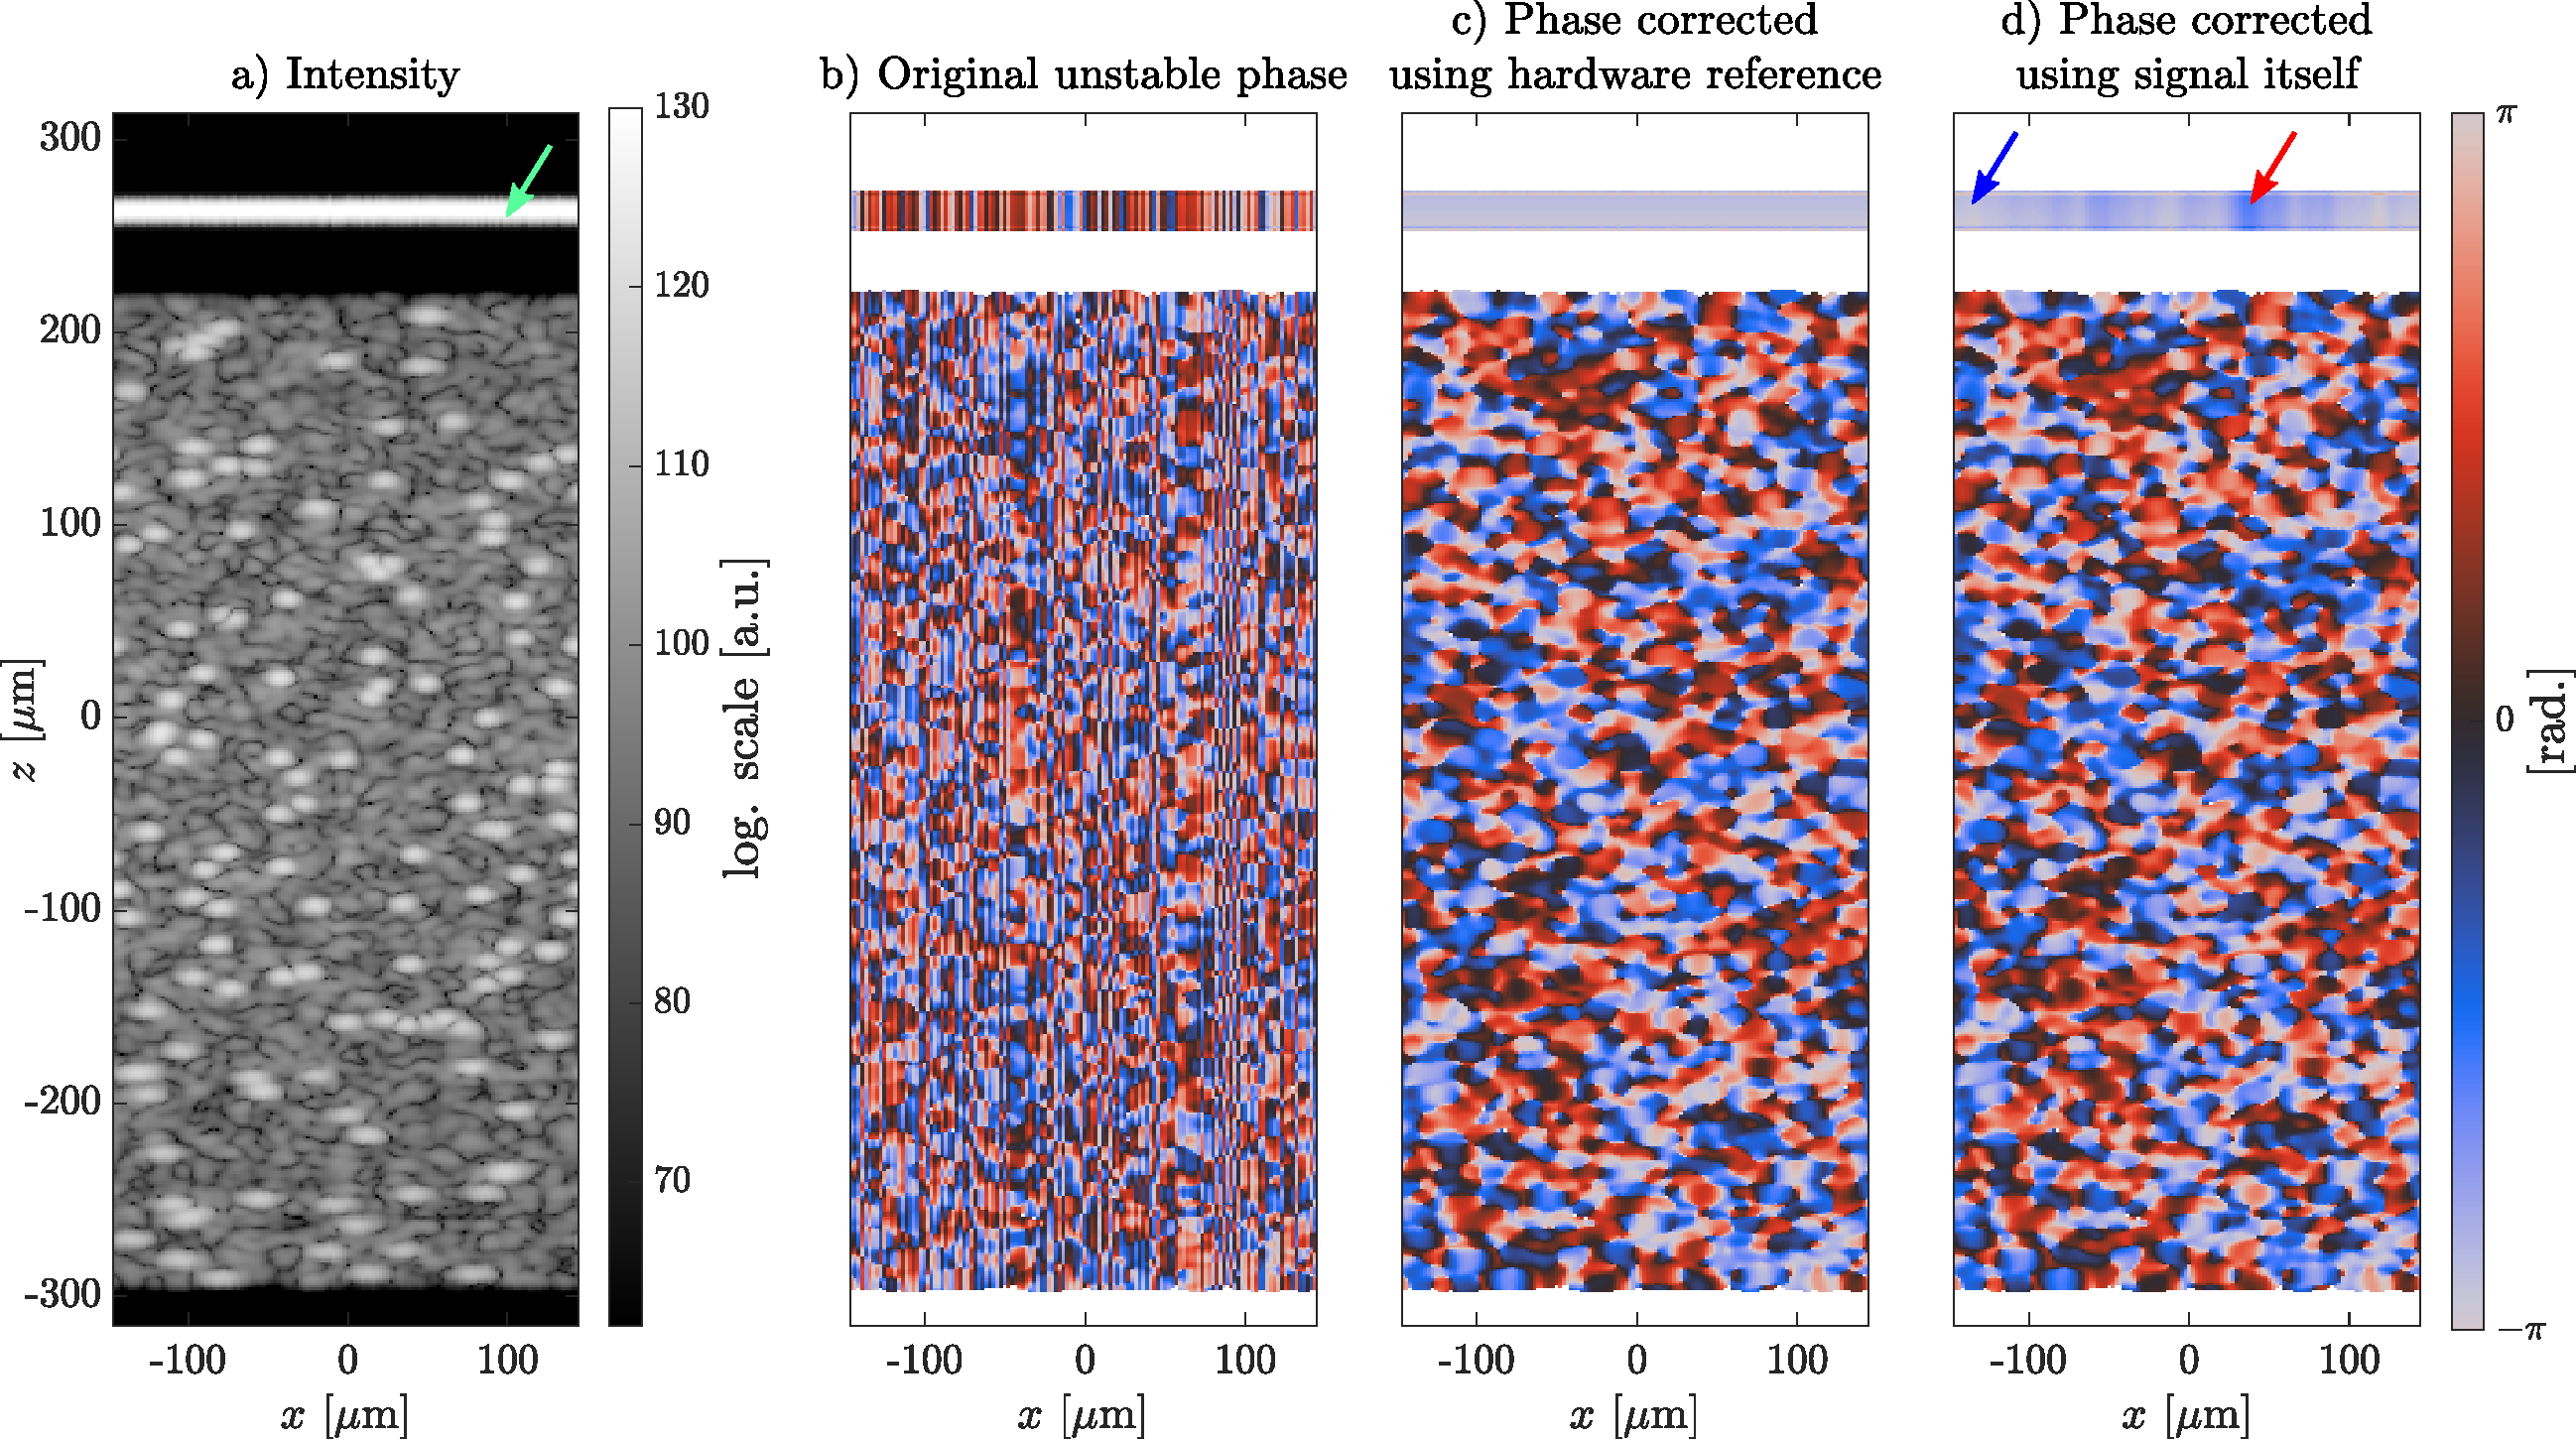
\includegraphics[width=\textwidth]{Figures/TheoreticalBasis/PhaseStabilizationComp.pdf}
	\caption[Illustration of phase stabilization.]{Illustration of phase stabilization. OCT image simulated using the forward model: (a) intensity and (b) phase presenting phase instabilities due to sample-induced phase noise. Corrected phase using (c) hardware reference and (d) tissue signal itself.}\label{fig:PhaseStabilization}
\end{figure}

Apart from the sample, a flat reflector marked by the green arrow in Fig.~\ref{fig:PhaseStabilization}(a) was added in the top of the image covering the whole fast scan axis but with a small thickness of $10~\mu$m. Note that phase of the reference reflector in Fig.~\ref{fig:PhaseStabilization}(b) appears constant along depth because no motion artifacts affects this direction, but it fluctuates randomly across the transverse axis due to sample-induce phase noise. This reference reflector was used to perform phase stabilization and the resultant corrected phase shown in Fig.~\ref{fig:PhaseStabilization}(c) exhibits a random but smooth behavior distinctive of correlated speckle, and the phase of the reference reflector is now constant as expected in a phase stable system.

Finally, the original unstable phase was also corrected using the signal information along, ignoring the pixels occupied by the reference reflector in the calculation of the phase differences. Resultant corrected phase shown in Fig.~\ref{fig:PhaseStabilization}(d) looks fairly similar to that corrected using the reference signal, showing that indeed phase correction is possible using the sample signal alone. Imperfections of the method can be visualized in the phase of the reference reflector in Fig.~\ref{fig:PhaseStabilization}(d): at local scale phase is correlated as observed in the individual regions marked by arrows blue and red, but at global scale the phase is uncorrelated as noted when comparing the phase in these two regions, which in  principle should have the same value.

In the previous models, phase differences for phase stabilization were calculated along fast scan axis $x$ but the same procedure can be applied along the slow scan axis $y$. Since its operation is intrinsically 1D, fully numerical phase stabilization yields successful results only along a single axis at a time, and its imperfections hinder any 2D correction. It means that in the presence of 2D phase instabilities in $xy$, only one axis can be phase-corrected; the one along which phase differences are calculated. Furthermore, performing two successive corrections along each axis once at a time, e.g. correcting $x$ axis first and then $y$ axis, is not successful either because the global errors induced in the first correction makes impossible to correct along the second axis without destroying the phase stability in the first axis.

Apart from using a hardware reference signal which relies on physical modifications, there is not any fully numerical phase stabilization method capable of correcting phase noise in two dimensions. This limitation has been overcome using systems that provide at least phase stability along one scan axis~\cite{Ginner2017_Noniterative, Shemonski2014_Threedimensional, Fechtig2015_Highspeed, Ginner2018_Holographic, Leitgeb2016_Digital,Yasuno2006_Noniterative, South2019_Local}, in some cases even phase stability along the two scan axis is obtainable and therefore phase stabilization is unnecessary~\cite{Kumar2013_Subaperture, Hillmann2016_Aberrationfree, Pande2016_Automated, Kumar2015_Anisotropic,Sudkamp2018_Simple}. In particular, CAC techniques has been used mostly in SDOCT systems that have potential to provide 1D, or even 2D phase stability using fast line-field systems. In raster scan SDOCT systems, scanning speed along fast scan axis is fast enough to neglect motion artifacts in that direction, and phase offsets are only significant along the slow scan axis, this, in combination with numerical stabilization is sufficient for the operation of CAC techniques~\cite{Shemonski2014_Threedimensional}.

Numerical phase correction of phase-jitter noise is straightforward with extensions of the aforementioned phase stabilization methods, but they still provide 1D phase stability and no 2D phase correction is yet known. Because SSOCT are intrinsically 2D phase unstable in the presence of phase-jitter, CAC techniques in such systems have rely on hardware solutions. For instance, full-field systems have been used since they provide intrinsic 2D phase stability given the parallel acquisition of the entire transverse plane~\cite{Kumar2013_Subaperture, Hillmann2016_Aberrationfree}, and more recently operation in raster scan systems has been possible using $k$-clocked systems~\cite{Kumar2017_Invivo}. These solutions are considerably unpractical since they require major hardware components that are not present in most OCT systems. For instance, $k$-clocks require an additional interferometer and a compatible digitizer that not only increase cost but also complexity of the systems.

Computational aberration correction is a powerful tool in many scenarios but it has been very restricted by the phase stability requirement; it is not possible to carry out any CAC technique in many raster scan OCT systems. There is therefore a great interest in developing a fully numerical strategies to perform CAC techniques in 2D phase unstable system.

In following chapter, a technique for CAO in 2D phase unstable systems developed in this work is described and succesful experimental demonstratations are presented.
\newpage
\phantomsection
%\chapter{Computational adaptive optics for phase unstable OCT systems}
\chapter[Computational aberration correction in phase-unstable OCT: SHARP]{Computational aberration correction in phase unstable OCT: SHARP}\label{chap:SHARP}

There are several techniques for computational aberration correction in OCT as presented in previous chapter, all relying on a phase stability requirement to successfully operate the complex OCT signal. The core proposal of this work is described in detail in this chapter, a technique called SHARP to carry out CAO in tomograms having two dimensional phase noise, capable of correcting $x$-$y$-separable aberrations in tomograms affected by phase-jitter noise, which typically appears as 2D phase noise. The foundation of the method are presented in Section~\ref{sec:SHARP}, starting with the description of a tool for the assessment of phase stability and the validation of Nyquist sampling, following with an illustration of attempts to 2D phase stabilization, to show the impossibility to succeed with current fully numerical correction and to explain the motivation behind the operation of SHARP, and by the end of the section, the steps of the method are described and explained in detail. Then, results from a proof of concept experiment are presented in Section~\ref{sec:Test}, to evaluate the performance of SHARP in experimental datasets and determine if its purposed is well accomplished. Finally, complementary steps for SHARP are explained in Section~\ref{sec:Extensions}, oriented to solve specific issues not covered by the general proposal, in order to increase its applicability and improve results in particular situations.

\section{SHARP: A CAO technique for OCT}\label{sec:SHARP}

\subsection{Phase stability and sampling assessment}

Although phase stability of a system can be roughly estimated by imaging an ideal reflective surface and computing the phase difference between consecutive A-lines, this is not useful in practical situations to estimate phase stability in tomograms of real samples unless there is a reference reflective surface. Here, a tool for qualitative assessing phase stability and sampling in any complex tomogram is presented, based on the sample signal information itself and its acquisition process, as devised in a previous work~\cite{Cuartas-Velez2017_Formacion}.

Consider the lateral Fourier transform of the acquired signal $\hat{S}(x,y;z_d)$ for the low-NA regime in Eq.~\eqref{eq:CAO}, which can be written as
\begin{equation}
    \hat{S}(q_x, q_y; z_d) = H(q_x, q_y, z_d) \hat{\eta}(q_x, q_y, z_d),
\end{equation}
where the phase term in Eq.~\eqref{eq:CAO} is included in the frequency filter $H$, that can be described as $H(q_x,q_y, z_d)=\Omega(q_x, q_y, z_d)e^{i\varphi(q_x, q_y, z_d)}$, being $\Omega(q_x, q_y, z_d)$ its amplitude and $\varphi(q_x, q_y; z_d)$ its phase. Although the phase of $H$ varies with depth, its amplitude can be approximated to be constant over depth, and it follows a Gaussian distribution in the case that the input collimated beam in the scan lens of the system is also Gaussian-distributed (as it is in standard systems), this can be noted in the amplitude term $e^{-q^2\alpha^2/4k^2}$ of the forward model in Eq.~\eqref{eq:f^2}. Now, the power spectrum $\xi = |\hat{S}|^2$ of the signal is
\begin{align}
    \xi(q_x, q_y, z_d) &= |H(q_x, q_y, z_d) \hat{\eta}( q_x, q_y, z_d)|^2 \nonumber\\
    &= |\Omega(q_x, q_y)e^{i\varphi(q_x, q_y, z_d)} \hat{\eta}(q_x, q_y, z_d)|^2 \nonumber\\
    &= |\Omega(q_x, q_y)|^2 |\hat{\eta}(q_x, q_y, z_d)|^2.
\end{align}

The power spectrum of the sample $|\hat{\eta}(q_x, q_y, z_d)|^2$ is in general unknown but it is known to be a random distribution, given the random scattering property that characterizes tissue. Therefore, the expected value over depth of $|\hat{\eta}(q_x, q_y, z_d)|^2$ will yield a flat, nearly constant power spectrum $\gamma$, thus the mean power spectrum (MPS) $\bar{\xi}$ of the acquired discrete signal, averaged over $N_z$ depths planes, is given by
\begin{align}
    \bar{\xi}(q_m, q_n) &= \frac{1}{N_z}\sum_{l=1}^{N_z}\left|\text{FT}_{m,n}\{S(m,n,l)\}\right|^2\nonumber\\
%    &\approx \frac{1}{N_z}\sum_{l=1}^{N_z}|\Omega(q_m, q_n)|^2 |\hat{\eta}(q_m, q_n, l)|^2 \nonumber\\
    &\approx \frac{1}{N_z}|\Omega(q_m, q_n)|^2 \sum_{l=1}^{N_z} |\hat{\eta}(q_m, q_n, l)|^2 \nonumber\\
    &\approx \frac{1}{N_z}\gamma|\Omega(q_m, q_n)|^2,
\end{align}
where $(q_m,q_n)$ are discrete indexes for $(q_x,q_y)$, and because $\Omega$ follows a Gaussian distribution, then \textbf{the MPS $\bar{\xi}$ is also expected to follow a Gaussian distribution}. However, the latter is true assuming that the are not phase or amplitude disturbances on the signal $S(x,y,z)$, implying that the MPS is indeed a potential tool to evaluate phase stability.

Phase noise affecting local phase stability manifests as high frequency disturbances in the OCT signal, thus the Fourier transform of the signal will be distorted, presenting more high-frequency content than expected and therefore the MPS will no longer follow a Gaussian distribution. In other words, \textbf{the MPS of a tomogram with local phase stability follows a Gaussian distribution} whereas the MPS of a tomogram with local phase instabilities follows a non-Gaussian distribution, approaching a flat distribution. This ``rule of thumb'' on the analysis of the MPS is useful to determine whether a certain tomogram has enough phase stability for a successful operation of any CAC technique.

In the presence of global or long-range phase noise, the MPS will be only slightly affected given that such phase noise manifests as low-frequency content that is less significant than the low-frequency content of the Gaussian function. Such observation is important given that numerical phase stabilization method described in Section~\ref{sec:phaseStabilization} yields only local phase stability and not global, yet the analysis on the MPS is valid for such case.

To visualize the previous explanations, Figure~\ref{fig:MPSExample} shows the MPS of the simulated tomogram used for Fig.~\ref{fig:CAO} that is intrinsically phase stable as shown in Fig.~\ref{fig:MPSExample}(a), and also the MPS after inducing phase noise consisting in phase offsets randomly distributed across A-lines to illustrate the MPS of a phase-unstable tomogram, which has a nearly flat distribution as observed in Fig.~\ref{fig:MPSExample}(b). Although the phase-stable MPS in Fig.~\ref{fig:MPSExample}(a) approximates to a Gaussian function, residual non-constant contributions of the sample frequency content appears when not sufficient depth planes $N_z$ are available (in this case $N_z = 256$). This, however, do not prevent the analysis on the MPS in practical terms because the Gaussian distribution dominates.

\begin{figure}[htb!]
	\centering
	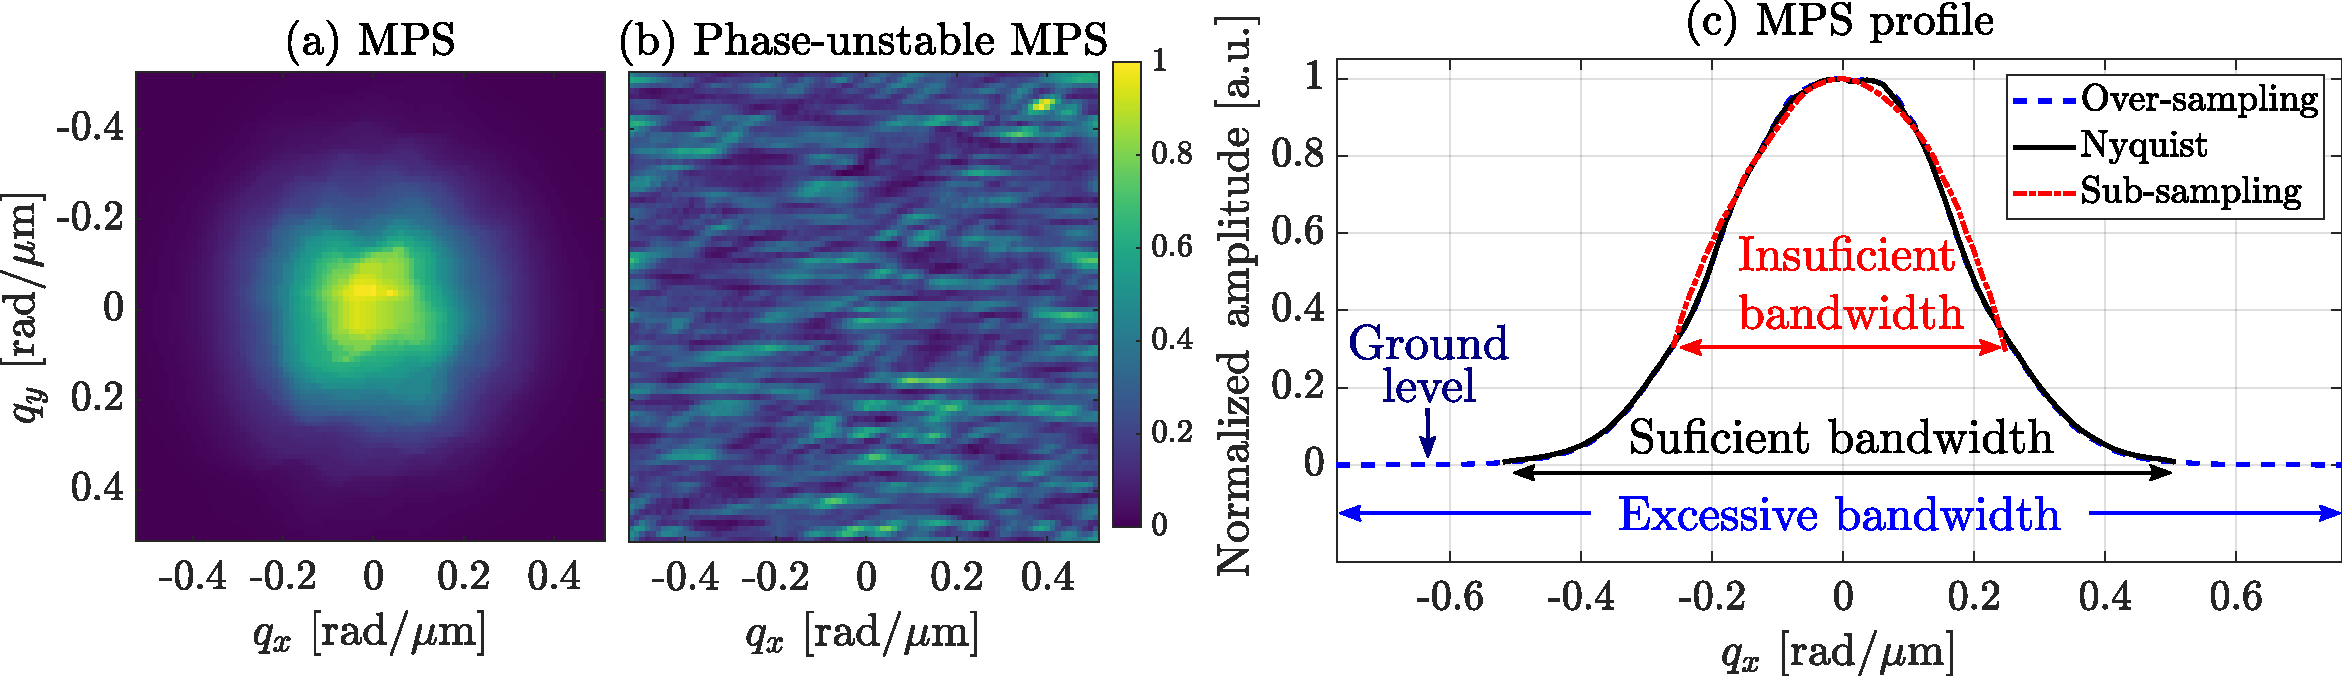
\includegraphics[width=\textwidth]{Figures/SHARP/PhaseStabilization/MPSExample.pdf}
	\caption[Illustration of the mean power spectrum with a simulated OCT tomogram.]{Illustration of the mean power spectrum with a simulated OCT tomogram. (a) MPS of raw tomogram, (b) MPS of tomogram with induced phase noise, and (c) 1D profile of the MPS averaging along $q_y$, for the tomogram using different samplings.}
	\label{fig:MPSExample}
\end{figure}

On the other hand, given the importance of a correct sampling for the operation of CAC techniques, it is worth to discuss the impact of sampling on the MPS, depicted in Fig.~\ref{fig:MPSExample}(c). Gaussian shape of the MPS is related to the fact that the optical system acts as a low-pass filter with cutoff frequency $f_c$ defined by the spatial resolution, thus the bandwidth of the Gaussian function is determined by the spatial resolution. The MPS will be truncated depending on the sampling, therefore changing sampling will not change the width of the Gaussian MPS, it will just truncate the Gaussian distribution depending on the sampling frequency. A \textit{correct/incorrect} sampling of the tomogram will result in a \textit{sufficient/insufficient} frequency bandwidth of the Gaussian-shaped MPS. as it is explained below.

It is known that Nyquist frequency $f_N = 2f_{\text{max}}$ provides the sufficient frequency bandwidth to correctly sample a signal with a known maximum frequency $f_{\text{max}}$, which in this case is determined by the lateral resolution $f_{\text{max}} = 1 / \delta x$, thus $f_N=2/\delta x$. In the case of having a correctly sampled tomogram (i.e. sampling less than $\delta x$/2), the frequency content will extend at least or beyond $f_c$, which means that the frequency bandwidth is \textit{sufficient} to capture the Gaussian shape of the MPS, as occurs in blue and black curves in Fig.~\ref{fig:MPSExample}(c) corresponding to the MPS of over-sampled and Nyquist-sampled tomograms, respectively. In the opposite case of having an incorrectly sampled tomogram (sampling greater than $\delta x$/2) the frequency content will be truncated before $f_c$, thus the frequency bandwidth is \textit{insufficient} to capture the Gaussian shape of the MPS, as occurs with red curve in Fig.~\ref{fig:MPSExample}(c) that corresponds to the MPS of a sub-sampled tomogram, which do not reaches the ground level, contrary to the other two curves. Therefore, \textbf{a tomogram with correct sampling will exhibit a MPS that captures the entire effective bandwidth of its Gaussian shape}, this means that the high frequency content reaches the ground level, which is essentially zero but in practical terms will be the noise floor level.

The two previous analysis on the MPS are therefore useful tools to determine that certain tomogram satisfies the two main requirements for successful operation of CAC techniques: phase stability and fulfillment of Nyquist theorem~\cite{Ruiz-Lopera2020_Computational}. The MPS can be used to analyze the phase stability provided by the fully numerical phase stabilization method described in Section~\ref{sec:phaseStabilization} that is of particular interest here. To do so, the simulated phase-unstable dataset used to exemplify the MPS in Fig.~\ref{fig:MPSExample} was corrected using the phase differences of A-lines along $x$ to compute the phase-jumps correction. Figure~\ref{fig:PhaseStable1D-enface} shows \textit{en face} phase images of the original tomogram, that is intrinsically phase stable [Fig.~\ref{fig:PhaseStable1D-enface}(a)], of the tomogram with induced random phase-jumps, that is 2D phase-unstable [Fig.~\ref{fig:PhaseStable1D-enface}(b)] and after correcting phase-jumps along $x$ axis, resulting in phase stability only along this axis [Fig.~\ref{fig:PhaseStable1D-enface}(c)]. The original tomogram is 2D phase-stable as indicated by the 2D Gaussian shape of its MPS shown in Fig.~\ref{fig:PhaseStable1D-enface}(d), whereas phase-corrupted tomogram exhibits a nearly flat MPS in the two axes as shown in Fig.~\ref{fig:PhaseStable1D-enface}(e). Instead, the phase-corrected tomogram exhibits 1D phase stability, and this yields a MPS with Gaussian shape only along one axis, in this case $x$ axis, whereas the orthogonal dimension remains phase unstable and thus with a flat MPS as depicted in Fig.~\ref{fig:PhaseStable1D-enface}(f). To verify that indeed 1D phase stability is achieved after correction, the 1D profile of the MPS in $x$ axis can be computed by averaging along $q_y$ axis, and this is shown in Fig.~\ref{fig:PhaseStable1D-enface}(e), where the 1D MPS of the original and phase-corrected tomograms approximate to a similar Gaussian shape, but corrupted tomogram has a constant MPS. Equivalent results are obtained if phase correction is computed using phase differences of A-lines along $y$ axis instead of $x$ axis, except that now the only phase-stable axis will be $y$.

\begin{figure}[htb!]
	\centering
	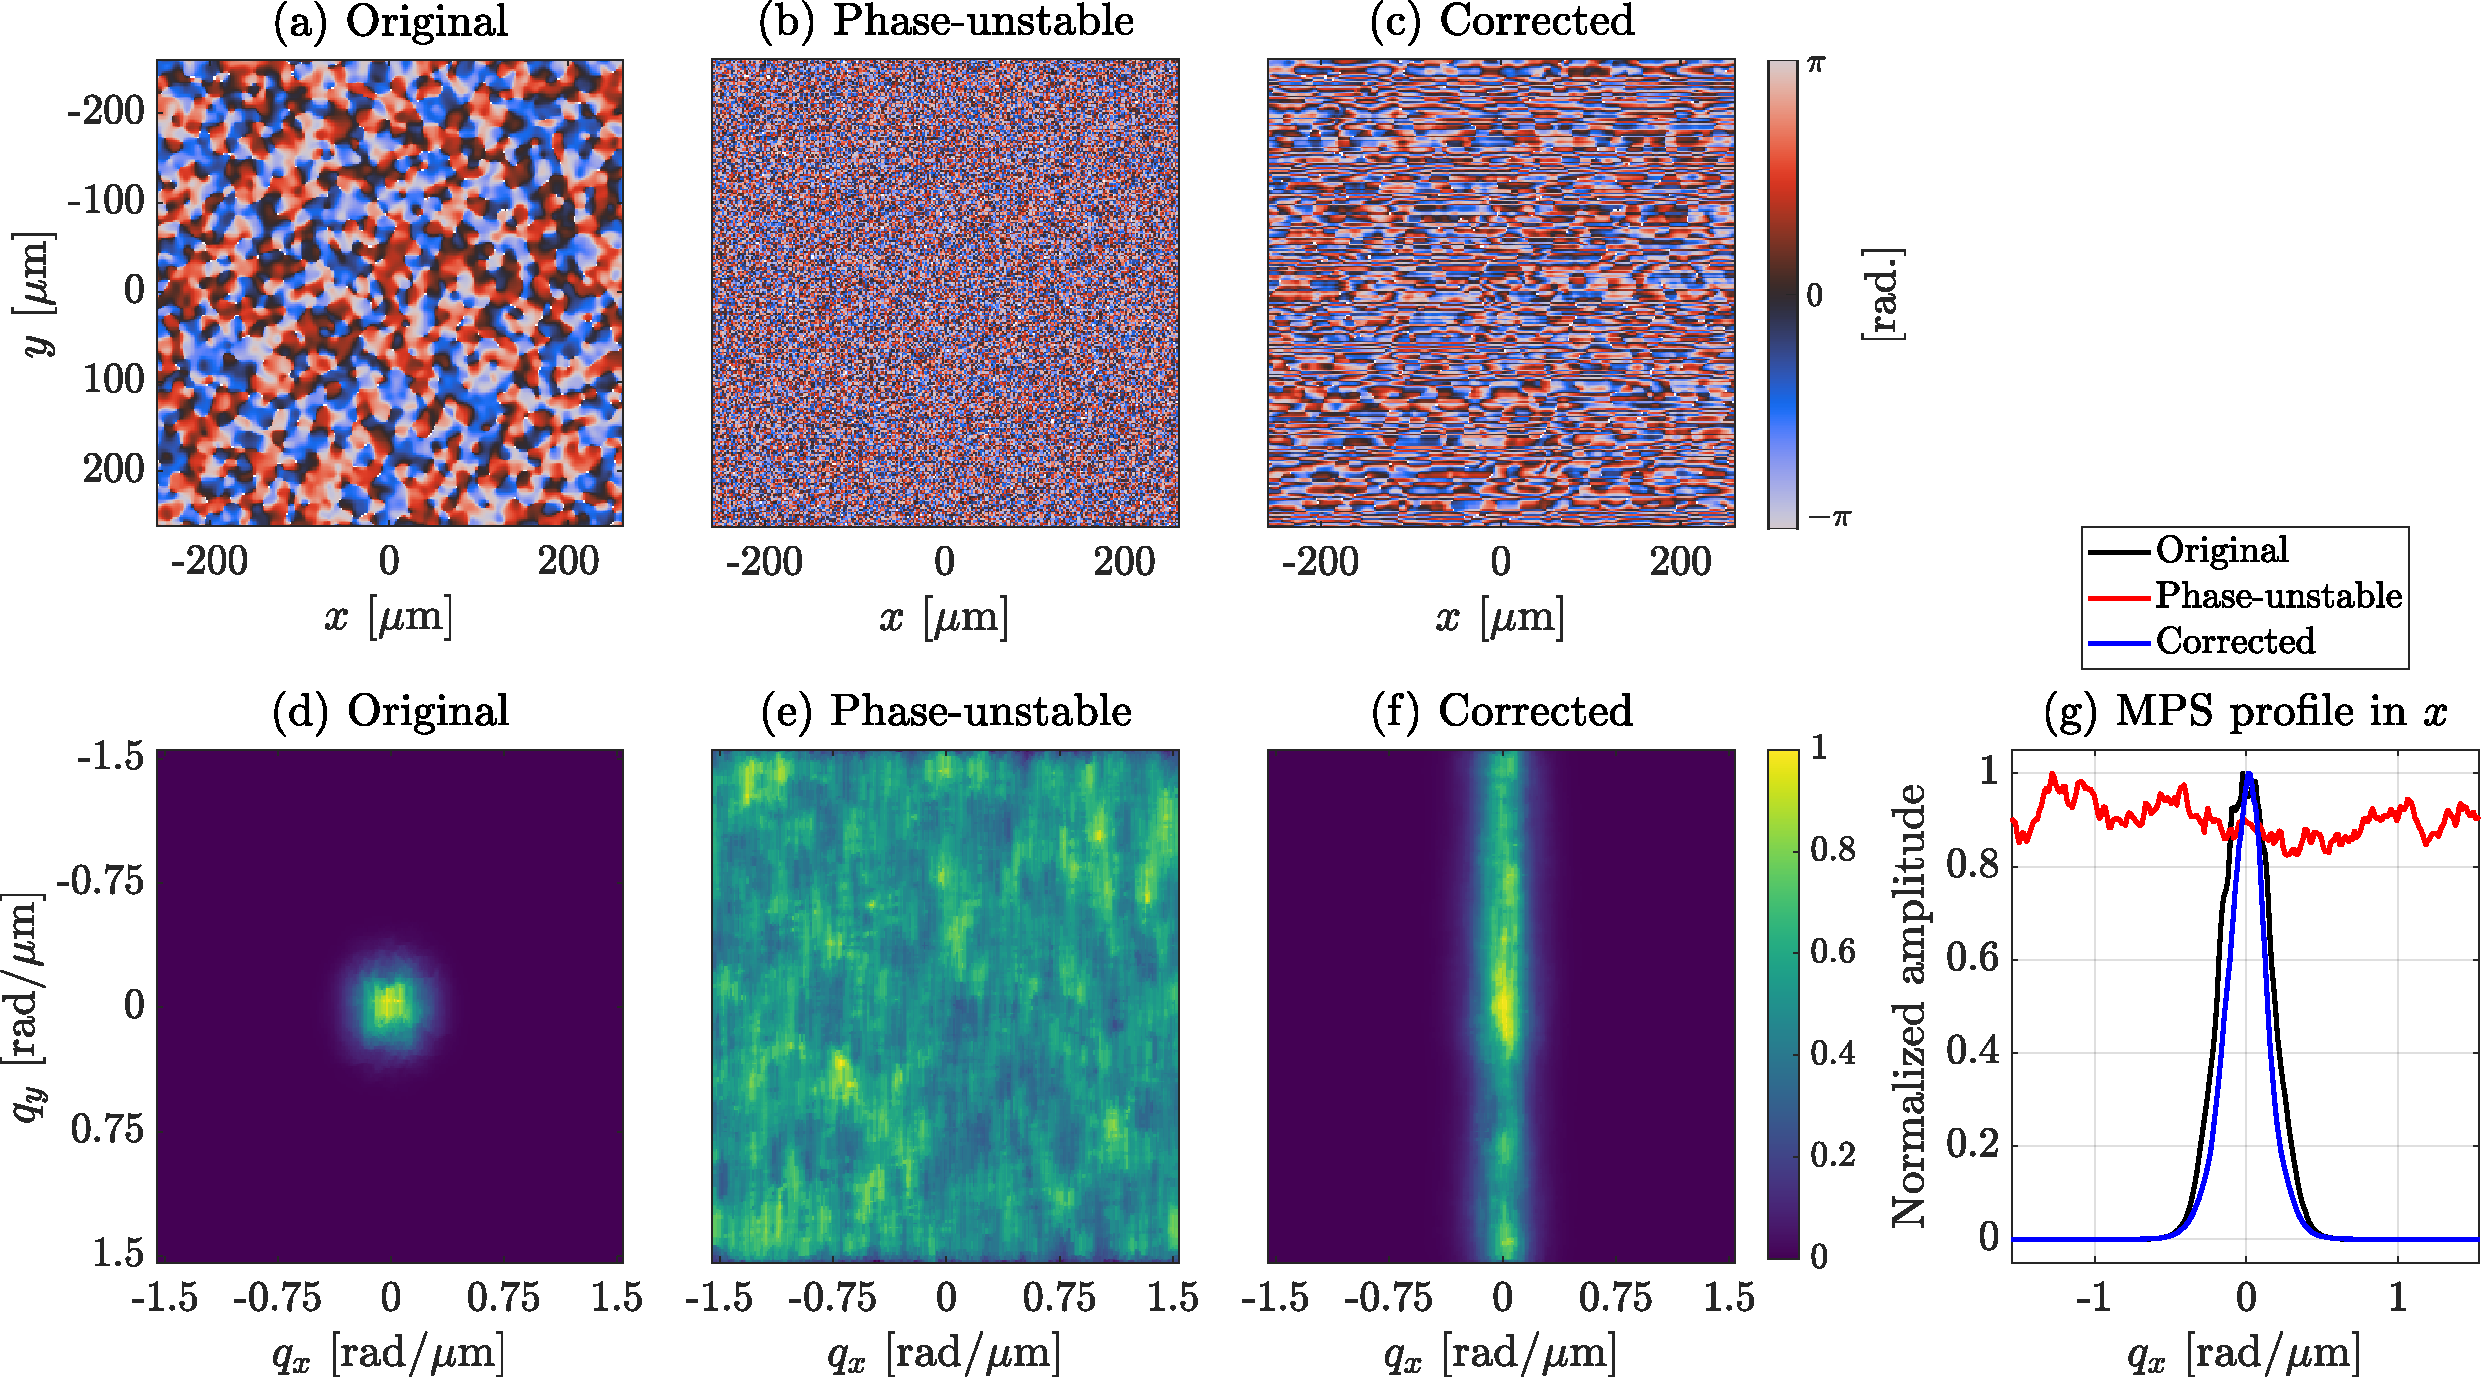
\includegraphics[width=\textwidth]{Figures/SHARP/PhaseStabilization/PhaseStabiliaztion1D-enface.pdf}
	\caption[Illustration of the mean power spectrum after phase correction with a simulated OCT tomogram.]{Illustration of the mean power spectrum after phase correction with a simulated OCT tomogram. \textit{En face} phase images: (a) original, (b) phase-unstable with random phase-jumps and (c) phase corrected along $x$. (d)-(f) MPS images of (a)-(c), respectively. (g) 1D profile of the MPS by averaing (d)-(f) along $q_y$.}
	\label{fig:PhaseStable1D-enface} 
23

\end{figure}
\FloatBarrier

\subsection{Attempts to 2D phase stabilization}

The presence of 2D phase noise requires a 2D correction but the fully numerical phase stabilization described previously is insufficient since its operation is intrinsically 1D. Two particular expansions of the phase stabilization method could be devised in order to achieve 2D phase stability, however, it is shown here that such attempts do not succeed as well as any stabilization based on traditional 1D phase correction.

First intuitive attempt to 2D phase stabilization is to perform two successive 1D phase corrections along the two scan axes. However, it has been found that the second correction would destroy the first correction hence, at the end, phase stability is achieved only along the axis that was corrected last. Results from this proposal were obtained using the phase-unstable simulated dataset used for Fig.~\ref{fig:PhaseStable1D-enface} and are illustrated in Figure~\ref{fig:PhaseStable2D} showing cross-sectional images of the plane $z$-$x$ (B-scan) and the orthogonal plane $z$-$y$. The phase-unstable tomogram was corrected along $x$ axis and resulting cross-sectional views are shown in Figs.~\ref{fig:PhaseStable2D}(a) and (b), exhibiting phase stability in the plane $z$-$x$ but not in the plane $z$-$y$. After the first correction, phase was corrected along $y$ axis expecting to obtain 2D phase stability but instead phase is corrupted again in the plane $z$-$x$ and only the plane $z$-$y$ is stable, as shown in Figs.~\ref{fig:PhaseStable2D}(c) and (d) which demonstrate that two consecutive 1D phase stabilization is not suitable to correct 2D phase noise. Because B-scan phase images are representative of a single plane, it is useful to analyze the MPS in order to know the general behavior of the entire tomogram. The $x$ and $y$ profiles of the MPS of the tomogram corrected only in $x$ and the one corrected in both axes are shown in Figs.~\ref{fig:PhaseStable2D} (g) and (h). Note that the MPS of the tomogram corrected only along $x$ is phase stable in this axis [black curve in Fig.~\ref{fig:PhaseStable2D}(g)] but it is phase unstable in $y$ axis [black curve in Fig.~\ref{fig:PhaseStable2D}(h)], contrary to the MPS of the tomogram corrected consecutively along the two axes [red curves in Figs.~\ref{fig:PhaseStable2D}(g) and (h)].

% \begin{figure}[htb!]
% 	\centering
% 	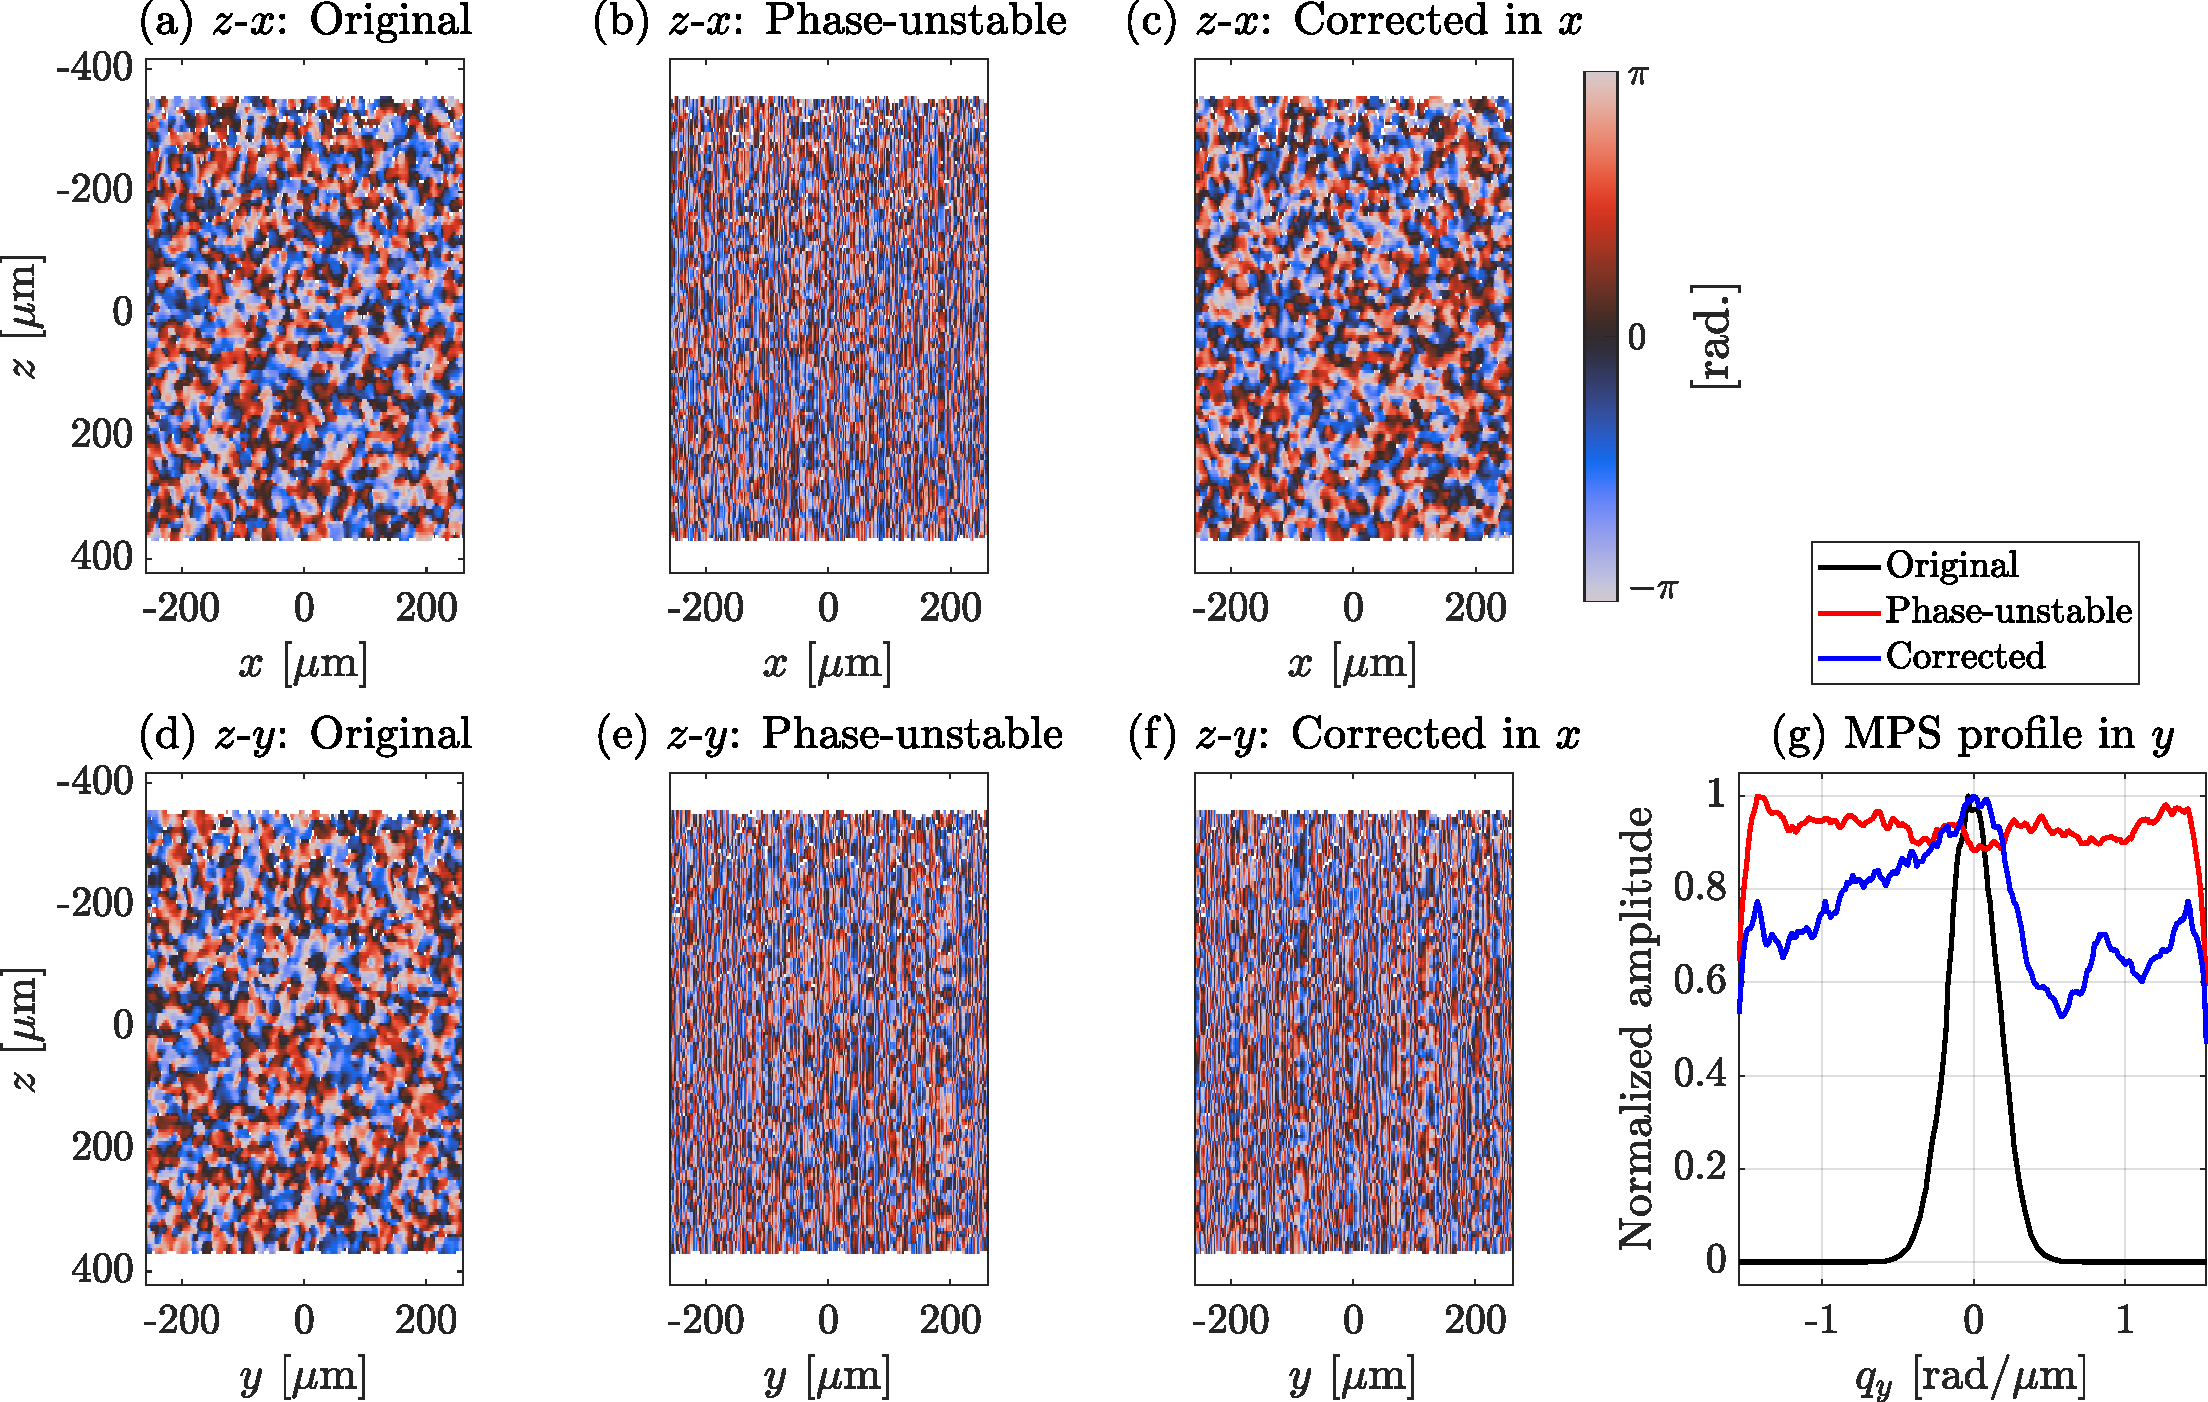
\includegraphics[width=\textwidth]{Figures/SHARP/PhaseStabilization/PhaseStabiliaztion1D.pdf}
% 	\caption[]{}
% 	\label{fig:PhaseStable1D}
% \end{figure}

\begin{figure}[htb!]
	\centering
	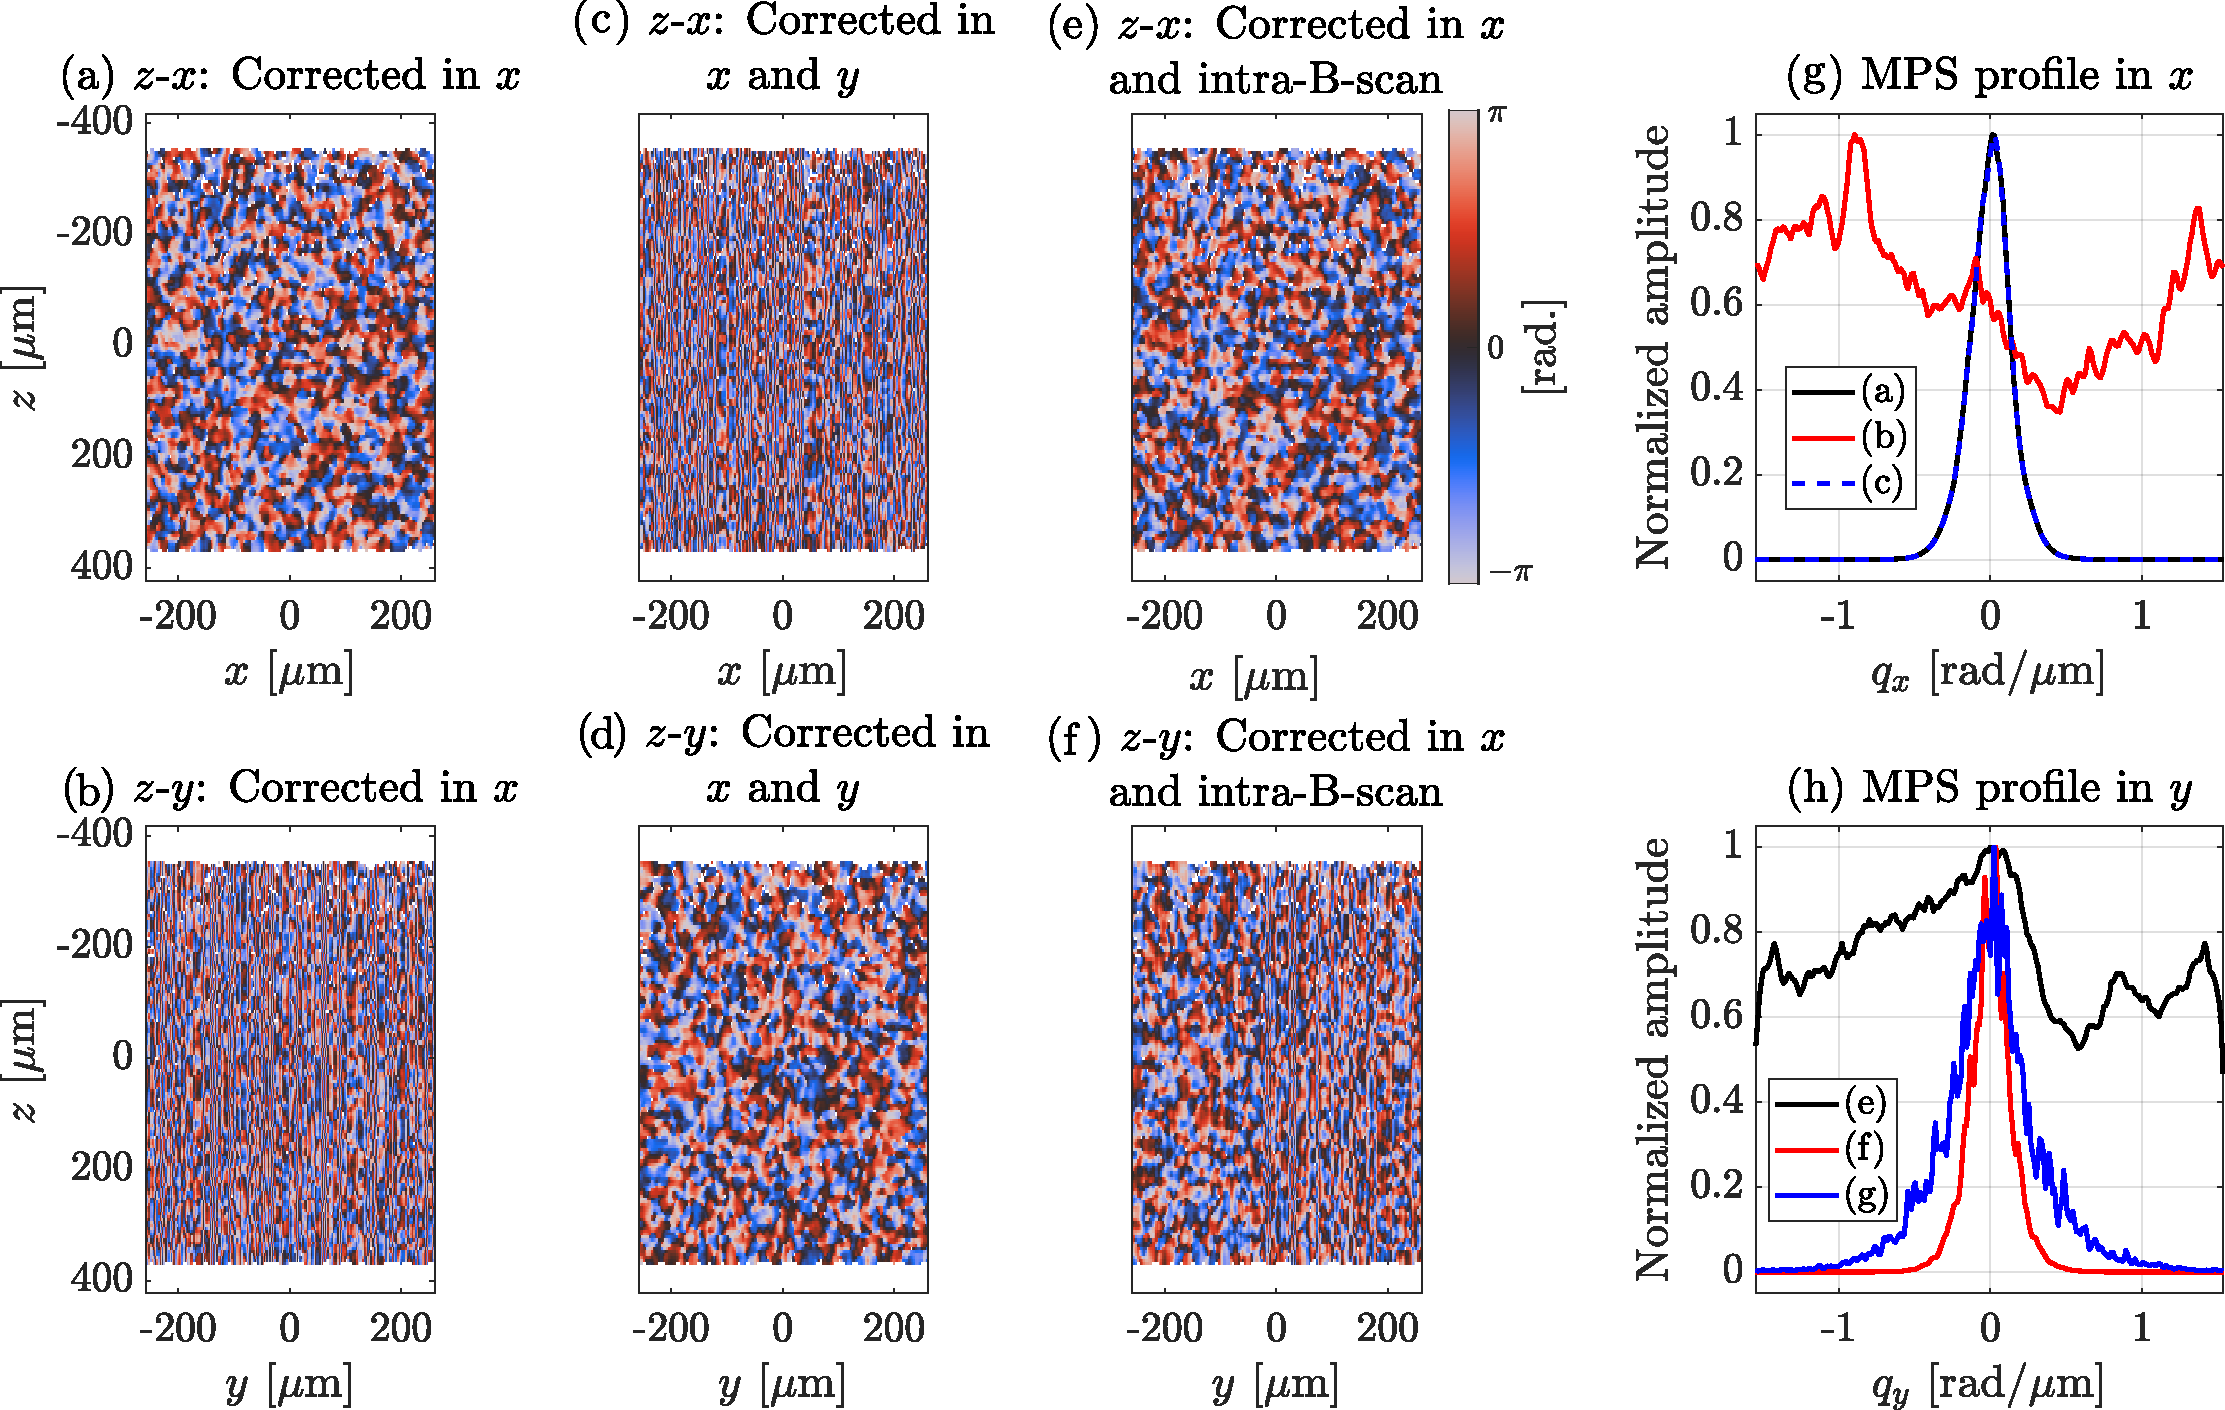
\includegraphics[width=\textwidth]{Figures/SHARP/PhaseStabilization/PhaseStabiliaztion2D.pdf}
	\caption[Illustration of attempts to 2D phase stabilization with a phase-unstable simulated dataset.]{Illustration of attempts to 2D phase stabilization with a phase-unstable simulated dataset. Cross-sectional views of: (a)-(b) tomogram corrected along $x$ axis, (c)-(d) tomogram corrected along $x$ axis and then along $y$ axis, (e)-(f), tomogram corrected along $x$ axis and then inter-B-scan. (a),(c),(e) are views of $z$-$x$ planes and (b),(d),(f) of $z$-$y$ planes. 1D Profile of the MPS: (g) in $x$ axis and (h) in $y$ axis.}
	\label{fig:PhaseStable2D}
\end{figure}

A second attempt to 2D phase stabilization is to correct the phase along one axis, and then to correct only for residual global phase noise between consecutive planes in the orthogonal axis, and this way the first correction will not be destroyed as in previous proposal. For instance, if phase is corrected along $x$, resulting in the corrected tomogram $\tilde{S}(m,n,l)$, then the second correction would be computed using the phase difference between A-lines along $y$ axis, that are then averaged along $x$ axis to obtain a global correction for each B-scan, instead of obtaining an individual correction for each A-line. The global corrections $\Delta_n$ between B-scans (or simply inter-B-scan) are calculated as
\begin{align}
    \delta(n) &= \arg\left\{\sum_{l=1}^{N_z} \sum_{m=1}^{N_x} S(m,n,l) S^*(m,n-1,l)\right\} \nonumber\\
    \Delta(n) &= \sum_{\hat{n} = 1}^n\delta(\hat{n}),
\end{align}
and applied as
\begin{equation}
    \tilde{\tilde{S}}(m,n,l) = \tilde{S}(m,n,l) e^{-i\Delta(n)},
\end{equation}
where $N_x$ is the number of A-lines in $x$ axis and $N_z$ is the number of depth samples, also note that $\Delta(n)$ is a function of B-scan index $n$ only. The purpose of the inter-B-scan correction is to correct for errors along the second axis without destroying phase stability along the first axis since it is a global correction for each B-scan. The latter is well-accomplished as noted in the B-scan phase image in Fig.~\ref{fig:PhaseStable2D}(e) that was corrected in $x$ and then inter-B-scan, but the inter-B-scan correction seems insufficient to correct for phase noise along $y$ axis as noted in Fig.~\ref{fig:PhaseStable2D}(f), which appears to be phase stable only in the left portion of the image, but not towards the right region, suggesting that a global correction is not sufficient. This is also observed in the MPS profiles; MPS in $x$ axis [blue curve in Fig.~\ref{fig:PhaseStable2D}(g)] is almost identical to that corrected only along $x$, but MPS in $y$ axis [blue curve in Fig.~\ref{fig:PhaseStable2D}(h)] exhibits residual high frequency content that suggests significant residual phase noise.

The impossibility to correct for 2D phase noise using traditional 1D phase stabilization may arise because small local errors, insignificant for local phase stability, are induced in the process and they propagate along the orthogonal direction as a consequence of the cumulative sum used to compute the global corrections, resulting in long-range errors that randomly disrupt the phase along this axis and frustrate any attempt to obtain 2D phase stability using 1D corrections.

\subsection{Description of the method}

In order to enable the operation of CAC techniques in tomograms with 2D phase noise like those acquired with SS-OCT systems presenting phase-jitter, it is possible to develop a scheme that leverage from 1D phase stability instead of aiming to succeed in 2D phase stabilization which is so far not possible with traditional phase correction. Here a novel technique is proposed for computational correction of aberrations in OCT tomograms with 2D phase noise, that leverages from the fact that 1D short-range phase stability is sufficient to perform the deconvolution operation in which CAC techniques are grounded, from this arises the name of the technique \textbf{SH}ort \textbf{A}line-\textbf{R}ange \textbf{P}hase-stability adaptive-optics (SHARP)~\cite{Ruiz-Lopera2020_Computational}.

SHARP integrates sequential 1D numerical phase noise and aberration correction steps and can operate in tomograms with phase noise arising from phase-jitter, galvanometer scanners and sub-resolution sample axial bulk motion, as long as Nyquist sampling is fulfilled. SHARP is suitable for OCT systems with no special hardware phase reference signals nor specialized configurations that ensure phase stability along any scan axis like those used often in the context of CAO, in particular, it is compatible with standard SS-OCT systems, affected by 2D phase noise.

The procedure consists in two sequential steps linked by an intermediate step as follows. First, phase noise is corrected along one axis $u$ (being $u$ either $x$ or $y$) followed by a 1D aberration compensation in that axis. Secondly, phase noise correction in $u$ is rolled-back by applying the inverse correction to the 1D \emph{corrected} tomogram. Then, phase noise is corrected along the other axis $v$, orthogonal to $u$, followed by a 1D aberration compensation in $v$, yielding a 2D computationally aberration-corrected volume. The intermediate rollback (RB) step is a key step to remove the long-range phase errors introduced in the first correction that would frustrate the second phase correction, and thus it enables the second CAC step.

A flowchart summarizing the procedure is shown in Figure~\ref{fig:SHARPFlowDiag}. $S_{m,n,l}$ is the input aberrated, phase-unstable tomogram, $\mathbb{C}_u\left\{\cdot\right\}$ represents the phase stabilization procedure applied along a generic axis $u$  and $\mathbb{C}_u^{-1}\left\{\cdot\right\}$ is its inverse meaning that the inverse phase correction is applied to cancel out the initial correction, $\mathbb{A}_u\left\{\cdot\right\}$ represents the aberration correction procedure applied along a generic axis $u$, and $\tilde{S}^{\text{1D}}_{m,n,l}$ and $\tilde{S}_{m,n,l}$ are the output, aberration-corrected tomograms, being $\tilde{S}_{m,n,l}$ the two-dimensional corrected tomogram that is the general interest, and $\tilde{S}^{\text{1D}}_{m,n,l}$ the one-dimensional aberration-corrected tomogram that is the aim in certain applications where 2D aberration correction is not possible for specific reasons subject to the application, for instance in catheter-based imaging. An optional, additional step is to rollback the second phase noise correction, thus recovering the original phase unstable tomogram but with aberrations already corrected, and this could be useful to combine SHARP with other phase-dependent techniques that would be carried out after application of SHARP.

\begin{figure}[htb!]
	\centering
	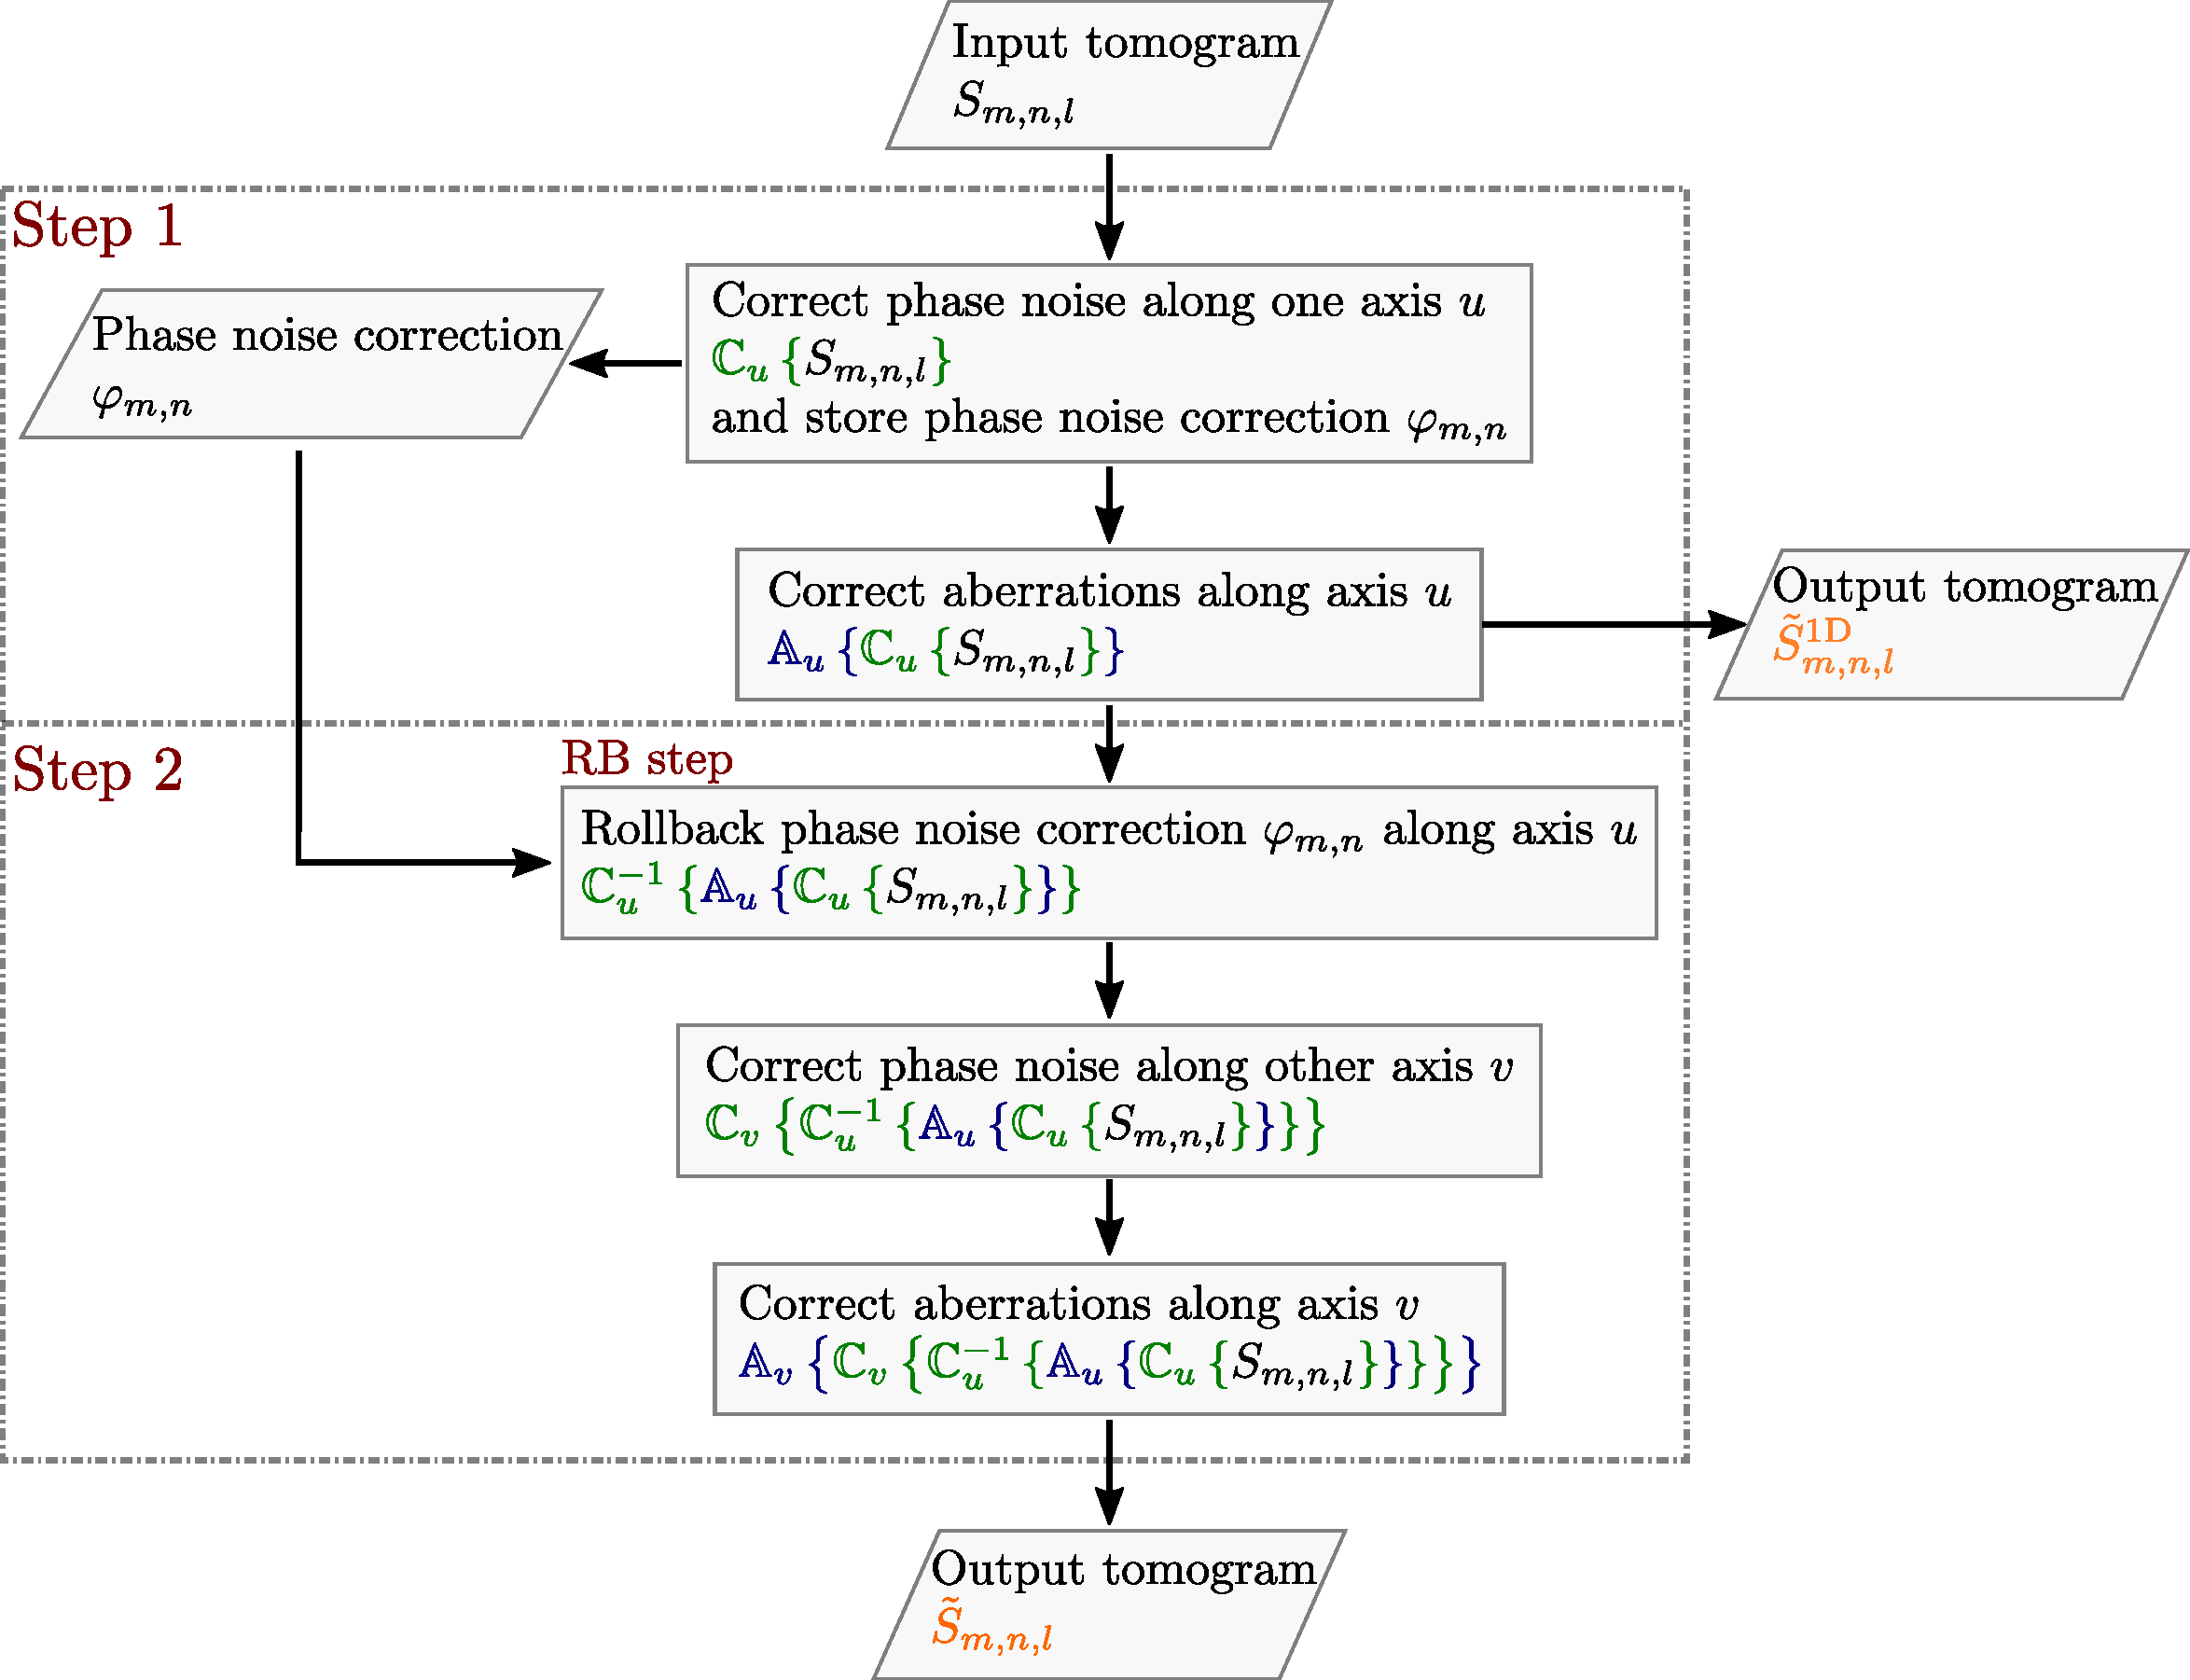
\includegraphics[width=\textwidth]{Figures/SHARP/BlockDiagram.pdf}
	\caption[Flowchart of the SHARP procedure.]{Flowchart of the SHARP procedure.}
	\label{fig:SHARPFlowDiag}
\end{figure}
\FloatBarrier

\subsubsection{Phase noise correction}

For the phase noise correction steps, a modification of the fully numerical method described in Section~\ref{sec:phaseStabilization} is used in order to address phase-jitter noise in addition to phase-offsets already covered by the method. The phase differences between consecutive A-lines along the axis of interest, for instance $x$ axis, are computed similarly to Eq.~\eqref{eq:PhaseDiff} as
\begin{equation}
    \delta(m,n,l) = \arg\left\{S(m,n,l)S^*(m-1,n,l)\right\}
\end{equation}
except that instead of summing along depth as in Eq.~\eqref{eq:PhaseDiff}, a linear fit of the form $\hat{\delta}(m,n,l) = b_0(m,n) + b_1(m,n)l$ is performed on $\delta(m,n,l)$ in order to estimate the phase offsets $b_0(m,n)$, arising from all potential sources such as galvanometer scanners or axial motion, as well as slopes $b_1(m,n)$ arising from phase-jitter noise. In other words, phase noise of each A-line is characterized by a phase-ramp noise with offset $b_0(m,n)$ and slope $b_1(m,n)$, with both parameters changing randomly across A-lines. Finally, phase correction operator $\mathbb{C}_x\left\{\cdot\right\}$ is applied to correct for phase-ramp noise as
\begin{align}\label{eq:phaseDiffJitterCor}
   \mathbb{C}_x\left\{S(m,n,l)\right\} &= e^{i\hat{\Delta}(m,n,l)} S(m,n,l) \nonumber\\ \text{where} \ \ \ \hat{\Delta}(m,n,l) &= \exp\left\{\sum_{\hat{m} = 1}^m \hat{\delta}(\hat{m},n,l)\right\}.
\end{align}

The exact same produce is applied to correct along $y$ axis, making $y$ as the variable of interest ($n$ in discrete notation). Logarithmic intensities of the conjugate products $10\log_{10}\left\{|S_{m,n,l}S^*_{m-1,n,l}|^2\right\}$ are used as weights to perform a weighted-linear fit. Furthermore, a mask is applied to ignore those pixels with logarithmic intensity below a threshold value, typically set to the noise floor level which in general can be approximated to be constant over the tomogram.

Given that the phase of a complex quantity is defined in the range [$-\pi,\ \pi$], phase wrapping may appear in Eq.~\ref{eq:phaseDiffJitterCor} if the phase-ramp exceeds these boundaries. It was already explained that phase wrapping is not an issue for phase-offsets correction (Section~\ref{sec:phaseStabilization}), but for the case of phase-slopes, wrapping can influence the linear fit, resulting in an erroneous correction. Therefore, phase unwrapping prior to the linear fit would be desirable to provide a more confident correction, however, it is challenging to perform an adequate phase unwrapping of the OCT signal given the presence of noise and speckle, and in practical terms it has been found that phase wrapping is not as critical as anticipated in this particular case. To clarify this, first consider that SS-OCT systems are equipped with a sampling clock to produce a trigger signal, typically using a fiber Bragg grating, so that the magnitude of phase-jitter is generally below one sampling cycle, equivalent to slopes below $2\pi$, being this the limit for phase wrapping, and timing jitter greater than two or three sampling cycles is seldom observed, in a standard system in normal conditions.

Furthermore, although imaging range of SS-OCT systems is typically of $\sim$6~mm, the effective axial range covered by tissue is in general equal or less than half the imaging range due to light absorption in the tissue. This means that the range where the phase-ramp is fitted is actually less than half the imaging range, reducing the susceptibility to phase-wrapping because only a portion of the ramp is used and not its entire extension. For instance, a timing jitter of two sample clocks results in a phase-ramp with effective range $4\pi$ in the full axial range but only with effective range $2\pi$ if the half axial range is used. Finally, before performing the linear fit, global phase offsets computed by averaging $\delta(m,n,l)$ along depth are subtracted to $\delta(m,n,l)$ in order to avoid the phase-ramp starting at a value where it could wrap.

Further experimental validation of SHARP will demonstrate that in practical terms these considerations and strategies are sufficient for the linear fit in the phase correction procedure despite the lack of phase unwrapping.

\subsubsection{Aberration correction: Phase filter}

For the aberration correction step, the idea behind SHARP is to perform two 1D independent corrections instead of a single 2D correction, given that only 1D phase stability is achieved in each phase noise correction step. This is possible assuming that the deconvolution process performed in CAC techniques can be separated into two 1D deconvolutions performed independently and sequentially, which is valid only for certain aberrations, more specifically for those aberrations represented by a deconvolution kernel that can be separated into two 1D kernels, called here as $x$-$y$-\textit{separable aberrations}. In SHARP, computational adaptive optics (CAO) approach (see Section~\ref{sec:CAO}) is adapted to a 1D operation. To do so, consider the expression for CAO in Eq.~\eqref{eq:CAO} written as
\begin{equation}
    \tilde{\eta}(x,y,z) = \text{FT}^{-1}_{q_x,q_y}\left\{\text{FT}_{x,y}\left\{S(x,y,z)\right\}H^{-1}(q_x,q_y,z)\right\},
\end{equation}
and assume that the complex filter $H(q_x,q_y,l)=H_{q_x}(q_x,z)H_{q_y}(q_y,z)$ is separable into two 1D complex filters, namely $H_{q_x}(q_x,z)$ and $H_{q_y}(q_y,z)$, that are applied independently using the 1D aberration correction operator $\mathbb{A}_x\left\{\cdot\right\}$ as
\begin{equation}
    \mathbb{A}_x\left\{S(x,y,z)\right\} = \text{FT}^{-1}_{q_x}\left\{\text{FT}_{x}\left\{S(x,y,z)\right\}H_{q_x}(q_x,z)\right\},
\end{equation}
where $x$ is the axis of interest, and similarly for $y$ axis by making $y$ as the variable of interest. The filter $H = \Omega e^{i\varphi}$ comprises amplitude $\Omega$ and phase $\varphi$. In CAO, the phase $\tilde{\varphi}$ that is an approximate estimation of the ideal and unknown phase $\varphi$ is defined in terms of a polynomial basis similarly to Eq.~\eqref{eq:PhaseDecomp}, but in SHARP a 1D polynomial basis $P_j$ is used instead of a 2D basis,
\begin{equation}
    \tilde{\varphi}(q_x,z) = \sum_{j=1}^K\vec{\alpha}_j(z)P_j(q_x)
\end{equation}
where $K$ is the number of polynomials used and $\vec{\alpha}_j(z)$ are the set of $K$ weights defined for each depth $z$. In SHARP, we use Legendre Polynomials $P_j$ (see \href{https://mathworld.wolfram.com/LegendrePolynomial.html}{Wolfram} or Ref.~\cite{Arfken2013_Legendre} for a quick revision if desired), being the first few orders
\begin{align*}
    P_0(x) &= 1 \\
    P_1(x) &= x \\
    P_2(x) &= \frac{1}{2}(3x^2 - 1) \\
    P_3(x) &= \frac{1}{2}(5x^3 - 3x) \\
    P_4(x) &= \frac{1}{8}(35x^4 - 30x^2 + 3) \\
    P_5(x) &= \frac{1}{8}(63x^5 - 70x^3 + 15x).
\end{align*}

There is not a 1D polynomial basis to describe aberrations, hence the choice of the polynomial basis is rather arbitrary because many basis will serve equally. For instance, defocus aberration can ideally be corrected with any quadratic polynomial ($P_2$ in Legendre's basis), but the weight value itself could vary from one basis to another. Zernike polynomials, the standard for description of aberrations, is a 2D basis thus it is not suitable for SHARP. In order to determine the optimal set of weights $\vec{\alpha}_j(z)$ that minimizes aberrations in the tomogram, SHARP employs an image sharpness quality metric based on the Shannon's entropy given by Eq.~\eqref{eq:SE}. This metric, widely used in CAO literature~\cite{Liu2011_Automatic, Liu2012_Digital, Hillmann2016_Aberrationfree} has been found to be robust to point objects  as well as extended objects which is appropriate for a reliable estimation of the optimal weights. The optimization procedure is carried out using the MATLAB's built-in function \textit{\href{https://www.mathworks.com/help/optim/ug/fminsearch.html}{fminsearch}} that employs the simplex algorithm~\cite{Lagarias1998_Convergence}.

\subsubsection{Amplitude filter}

The amplitude term $\Omega$ of the filter $H$ could be defined analytically based on the known properties of the probe beam, but this results in the amplification of undesired high-frequency noise because the inverse filter $\Omega^{-1}$ is applied in CAO. Given that amplitude term does not have a role in the correction of aberrations, but only in the signal strength, or equivalently in the signal-to-noise ratio (SNR), it is possible to simply use a unity-valued amplitude $\Omega = 1$~\cite{Yasuno2006_Noniterative,Hillmann2016_Aberrationfree,Adie2012_Computational}. There are, however, better approximations that aim to improve the results of the deconvolution process in terms of robustness to noise. An alternative, initially proposed for the restoration of astronomical images~\cite{Brault1971_Analysis}, is the so-called optimum filter (OF) that is constructed under the reasonable condition that the deviation of the noisy image $\tilde{I}(u) = I(u) + N(u)$ affected by noise $N(u)$ from the ideal noiseless image $I(u)$ should be minimum in the root-mean-square error sense~\cite{Bonet1999_High}, yielding the form of the OF as
\begin{equation}
    \tilde{\Omega}(q) = \frac{|\hat{I}(q)|^2}{|\hat{I}(q)|^2 + |\hat{N}(q)|^2},
\end{equation}
where $u$ is the variable in the measuring domain, $q$ is its conjugate in the Fourier domain, $\hat{I}(q)=\text{FT}_u\left\{I(u)\right\}$ and $\hat{N}(q)=\text{FT}_u\left\{N(u)\right\}$. Developed models for noise in OCT predict that noise is additive following a zero-mean Gaussian distribution, namely \textit{white} noise, thus its spectrum is flat, i.e. frequency-independent, which means that $|\hat{N}(q)|^2$ is nearly constant. Under the previous model, and because the noiseless signal is in general unknown, the OF can be rewritten as
\begin{equation}
    \tilde{\Omega}(q) = \frac{|\tildehat{I}(q)|^2 - |\hat{N}(q)|^2}{|\tildehat{I}(q)|^2},
\end{equation}
where $\tildehat{I}(q)=\text{FT}_u\{\hat{I}(u)\}$ is the Fourier transform of the measured noisy signal.

For the particular context of OCT, SHARP makes use of the MPS to define $|\hat{I}(q)|^2$, resulting in an smooth and overall filter for the entire tomogram. Given the 1D operation, the 1D MPS is used, obtained by averaging $\bar{\xi}(q_m,q_n)$ over the lateral axis that is not the interest, for instance averaging over $q_y$ as $\bar{\xi}_{q_m}(q_m) = \frac{1}{N_y}\sum_{q_n}^{N_y}\bar{\xi}(q_m,q_n)$ when filtering along $x$ axis, therefore the OF is
\begin{equation}
    \tilde{\Omega}(q_m) = \frac{\bar{\xi}_{q_m}(q_m) - \bar{\xi}_{q_m}(q_{N_m})}{\bar{\xi}_{q_m}(q_m)},
\end{equation}
where $|\hat{N}(q)|^2 = \bar{\xi}_{q_m}(q_{N_m})$ is an approximate estimation to the noise floor level assuming that the content of the MPS at the maximum frequency $q_{N_m}$ is dominated by noise, which is indeed valid given the Gaussian-shape of the MPS. In practice, rather than using directly the value at the maximum frequency, it is useful to average the value for a few more frequencies around it. The OF is an effective tool, not only to avoid amplification of high-frequency noise, but also to slightly reduce the noise floor level in the complex tomogram, and its application is straightforward since it is defined based on the data information alone; it is an adaptive filter. Handling noise is advantageous particularly for CAO because it is known that out-of-focus tomograms present lower SNR than in focus tomograms. 

An example of the optimum filter calculated for an ideal Gaussian MPS is depicted in Fig.~\ref{fig:OptimumFilter}. The amplitude of the filter is nearly constant and equal to one for the low frequency content where signal dominates, and decreases to zero towards the maximum frequency in order to filter out high-frequency components beyond the cutoff frequency that are dominated by noise.

\begin{figure}[htb!]
	\centering
	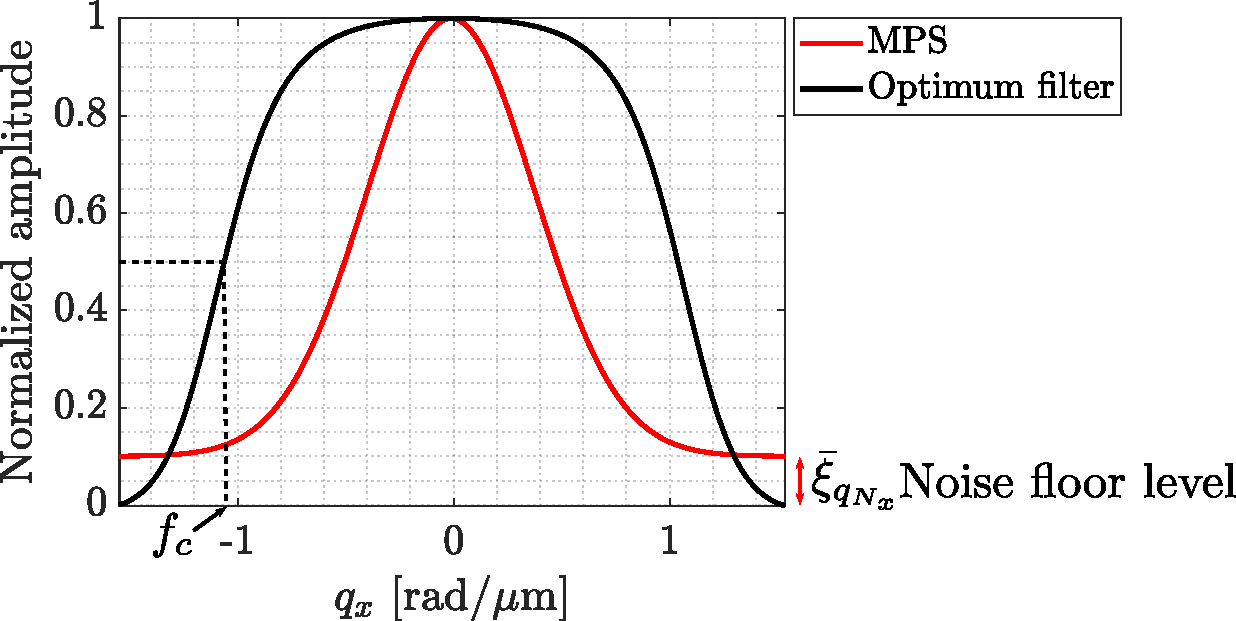
\includegraphics[width=.7\textwidth]{Figures/SHARP/OptimumFilterExample.pdf}
	\caption[Example of the optimum filter for a Gaussian MPS.]{Example of the optimum filter for a Gaussian MPS. $fc$: cutoff frequency of the filter.}
	\label{fig:OptimumFilter}
\end{figure}

Now that the phase stabilization and aberration correction procedures have been defined, the two 1D steps of SHARP can be condensed as
\begin{align}\label{eq:SHARP}
    \tilde{S}^{\text{1D}}(x,y,z) &= \mathbb{A}_x\left\{ \mathbb{C}_x\left\{ S(x,y,z) \right\} \right\}, \\
    \tilde{S}(x,y,z) &= \mathbb{A}_y\left\{ \mathbb{C}_y\left\{ \mathbb{C}^{-1}_x\left\{  \tilde{S}^{\text{1D}}(x,y,z) \right\} \right\} \right\},
\end{align}
where $\tilde{S}^{\text{1D}}(x,y,z)$ is the partially corrected tomogram and $\tilde{S}(x,y,z)$ is the $x$-$y$-separable aberrations corrected tomogram.

There are some particularities to discuss in regard to the described procedure. Because SHARP employs CAO, its operation is restricted to low-to-medium NA systems that is the regime of OCT. An extension to operate with high-NA systems could be possible by integrating ISAM in SHARP, however, this is the regime of OCM, which is not the aim in this work, and it is yet unclear whether ISAM procedure is compatible with 1D operation of SHARP.

The $x$-$y$ separability requirement has a direct limitation of the aberrations that can be corrected because not all aberrations can be separated into two 1D operations, only those whose deconvolution kernel can be separated into two 1D kernels. Among the $x$-$y$-separable aberrations, the most important for practical terms are defocus, $xy$-astigmatism and comma, being defocus the most relevant in many OCT applications given that it is intrinsic to the nature of the focused Gaussian beam used to illuminate the sample. In fact, defocus can be considered the only significant aberrations in many applications of OCT apart from retinal imaging where complex wavefronts may be induced by the eye of the subject. This means that SHARP is sufficient for many scenarios despite its $x$-$y$-separability requirement, in particular to numerically extend the depth of field, relaxing the trade-off between depth of field and lateral resolution.

Another important aspect is in regard to the role of the rollback step. The process of phase noise correction along the first axis adds random phase errors along the orthogonal axis that can become strong enough to frustrate the subsequent phase correction along the second axis, resulting in a lower local phase stability than the case of correcting the second axis directly, i.e. without correcting the first axis previously. The purpose of the RB step is to cancel out the first phase noise correction in order to avoid any strong error induced in the first correction. It can be noted that the RB step uses the phase noise correction computed before correcting aberrations along first axis but the RB itself is performed after correcting aberrations, which may change the phase pattern. Interestingly, the aberration correction applied along the first axis does not perturb the relative phase relation in the second axis although the phase pattern itself may have changed, hence the exact same phase noise correction is still valid for the RB (but conjugated) even though it is applied after aberration correction.

\section{Proof of concept experimental validation}\label{sec:Test}

To validate SHARP, an experiment was carried out in which a sample was imaged with a phase-unstable SSOCT system, inducing defocus on purpose by placing the focal plane of the scan lens outside the tissue thickness. A raster-scan non-$k$-clocked SSOCT system with a polygon-based wavelength-swept source was employed, similar to that in schematic Figure~\ref{fig:SSOCT_Scheme}. This custom-built system is affected by strong jitter in synchronization, as well as additional phase noise sources, such as the frequency shifter used to double the axial imaging range, that adds spurious phase offsets~\cite{Yun2004_Removing} and the galvo mirrors since the back-focal plane of the lens is not aligned with the pivot points of the galvos. The A-line repetition rate was $54$~kHz, in a $120$~nm $10$-dB-sweep spectral range centered at wavelength $1310$~nm. Light was focused onto the sample using a scan lens with transverse $e^{-2}$ beam diameter of $2w_0=22~\mu$m in a Rayleigh range of $z_R=290~\mu$m in air (Thorlabs LSM03, USA).

A \textit{cucumis sativus} sample was selected for the experiment as it displays prominent cellular walls with strong scattering, and large vacuoles with low scattering. The sample was imaged in a 3$\times$3~mm$^2$ lateral FoV within a ranging depth of 6~mm in air, acquiring 1024 samples per A-line, 512 A-lines per B-scan and 512 B-scans, for a total tomogram size of 1024$\times$512$\times$512 ($N_z\times N_x\times N_y$). A reference dataset was acquire placing the focal plane roughly 0.6~mm below the sample surface, referred to as \textit{in-focus} or reference tomogram, and the out-of-focus (OoF) dataset was acquired after shifting up the focal plane roughly 0.9~mm, thus located above the sample surface.

\begin{figure}[htb!]
	\centering
	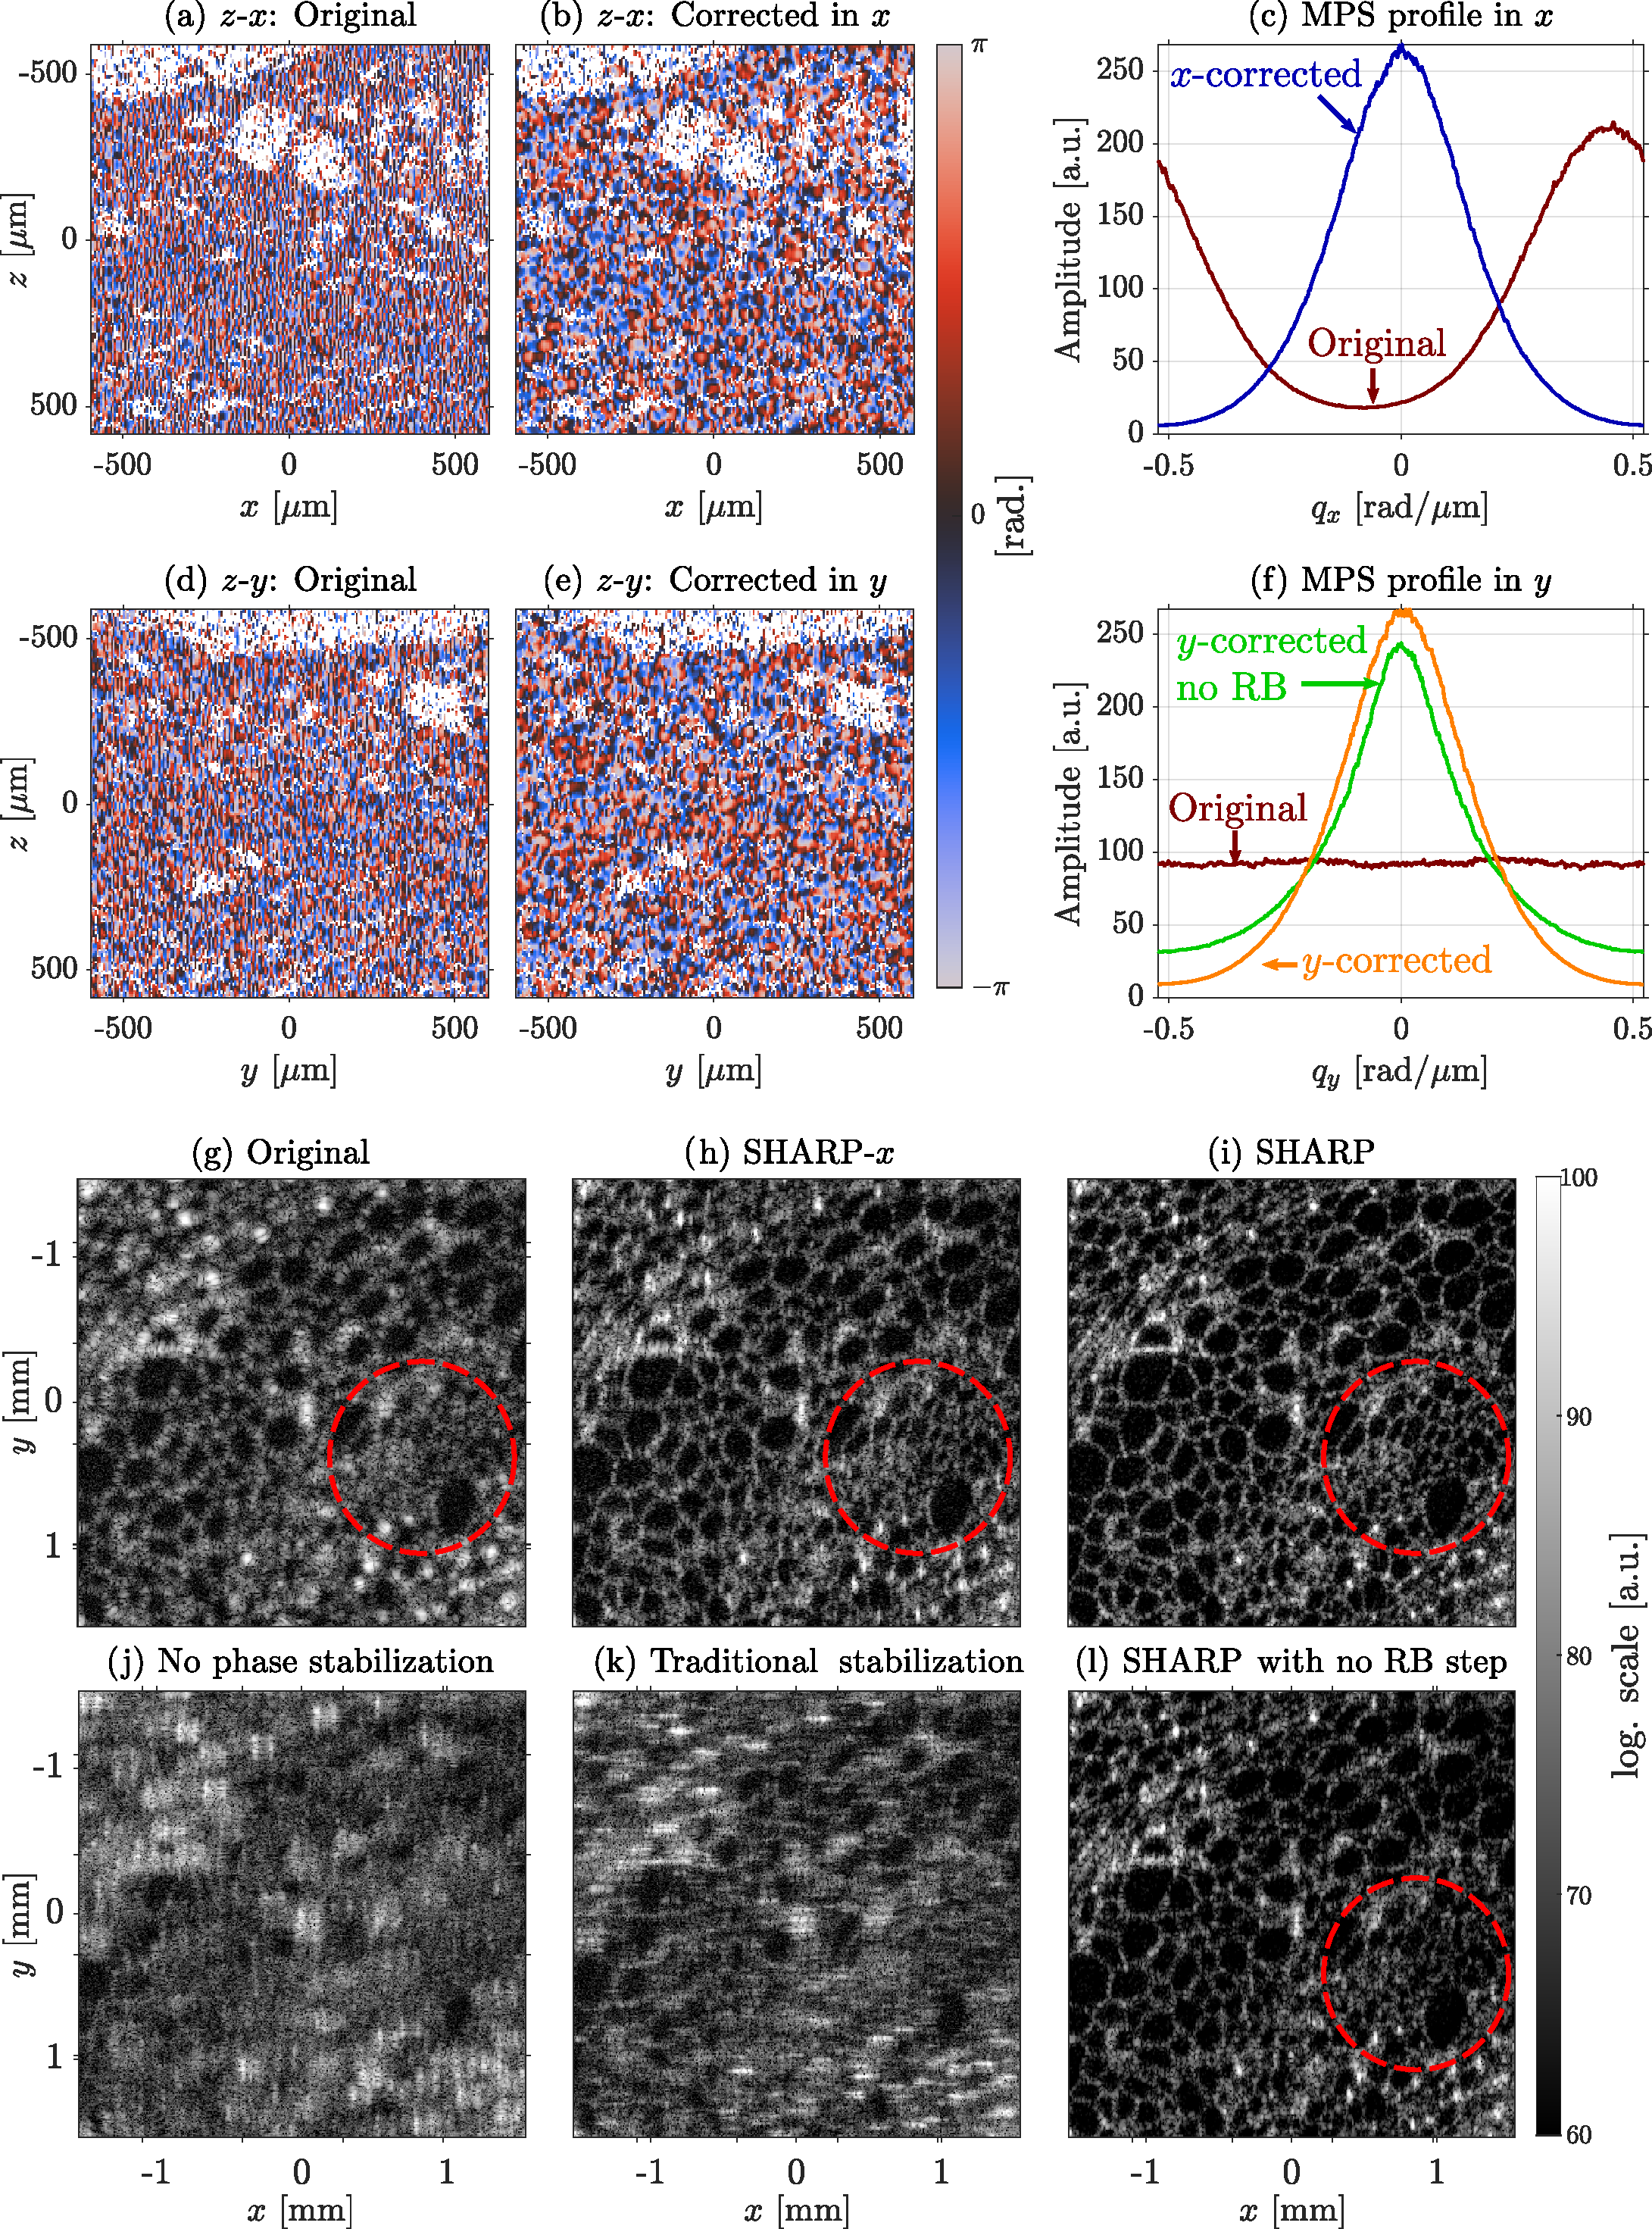
\includegraphics[width=.98\textwidth]{Figures/SHARP/SHARP_Cucumber.pdf}
	\caption[Proof of concept experimental validation of SHARP in a \textit{cucumis sativus} sample tomogram acquired with a SSOCT system.]{B-scan phase maps of \textit{cucumis sativus} sample in a small ROI; (a) before, (b) after $\mathbb{C}_x$ and (c) corresponding MPS profiles. $z$-$y$ phase maps; (d) before, (e) after $\mathbb{C}_y$ and (f) corresponding MPS profiles with and without RB step. Intensity \textit{en face} views; (g) original, (h) SHARP-$x$, (i)~SHARP, (l) SHARP without RB step, (j)~2D CAO with no phase stabilization and (k) with out-of-plane stabilization~\cite{Shemonski2014_Threedimensional}.}
	\label{fig:SHARP_Cucumber}
\end{figure}

SHARP was applied to the OoF tomogram using Legendre polynomial $P_2$ to describe the phase filter given that defocus is the only significant aberration in the experiment. Figure~\ref{fig:SHARP_Cucumber} illustrates results of each individual step of SHARP. A $z$-$x$ cross-sectional phase image in a small region of interest (ROI) of the raw unstable phase tomogram is shown in Fig.~\ref{fig:SHARP_Cucumber}(a), and after phase noise correction in $x$, or simply $\mathbb{C}_x$, in Fig.~\ref{fig:SHARP_Cucumber}(b), a point in which the MPS profile in $x$ exhibits a Gaussian shape and not a distorted one as original tomogram [Fig.~\ref{fig:SHARP_Cucumber}(c)]. After 1D CAO along $x$ axis (denoted as SHARP-$x$), the $zy$ plane remains phase unstable [Fig.~\ref{fig:SHARP_Cucumber}(d)], but after the RB step and $\mathbb{C}_y$, the $zy$ plane is now phase stable [Fig.~\ref{fig:SHARP_Cucumber}(d)] obtaining a MPS profile with Gaussian shape along $y$ [Fig.~\ref{fig:SHARP_Cucumber}(f)]. Without RB the MPS is distorted, approaching to a Gaussian function but with remnant high-frequency noise that suggests the presence of local phase instabilities that could frustrate CAO, as noted in the offset of green curve with respect to orange curve in Fig.~\ref{fig:SHARP_Cucumber}(f). Finally, a 2D refocused tomogram is obtained after applying 1D CAO in $y$.

Figures~\ref{fig:SHARP_Cucumber}(g)--(l) show intensity \textit{en face} views of the original tomogram, after SHARP-$x$ showing 1D refocusing only, after SHARP showing 2D refocusing and after SHARP without RB resulting in degraded quality of fine details, for instance in the region enclosed by the red circle, demonstrating the importance of the RB step. Additionally, results from failed attempts are illustrated; refocusing without any phase stabilization in Fig.~\ref{fig:SHARP_Cucumber}(j), showing destruction of signal information, and refocusing after phase stabilization only along out-of-plane axis in Fig.~\ref{fig:SHARP_Cucumber}(k), as is traditionally performed in SDOCT systems having in-plane phase stability~\cite{Shemonski2014_Threedimensional}, which also fails here because it is not sufficient for systems having 2D phase noise.

\begin{figure}[htb!]
	\centering
	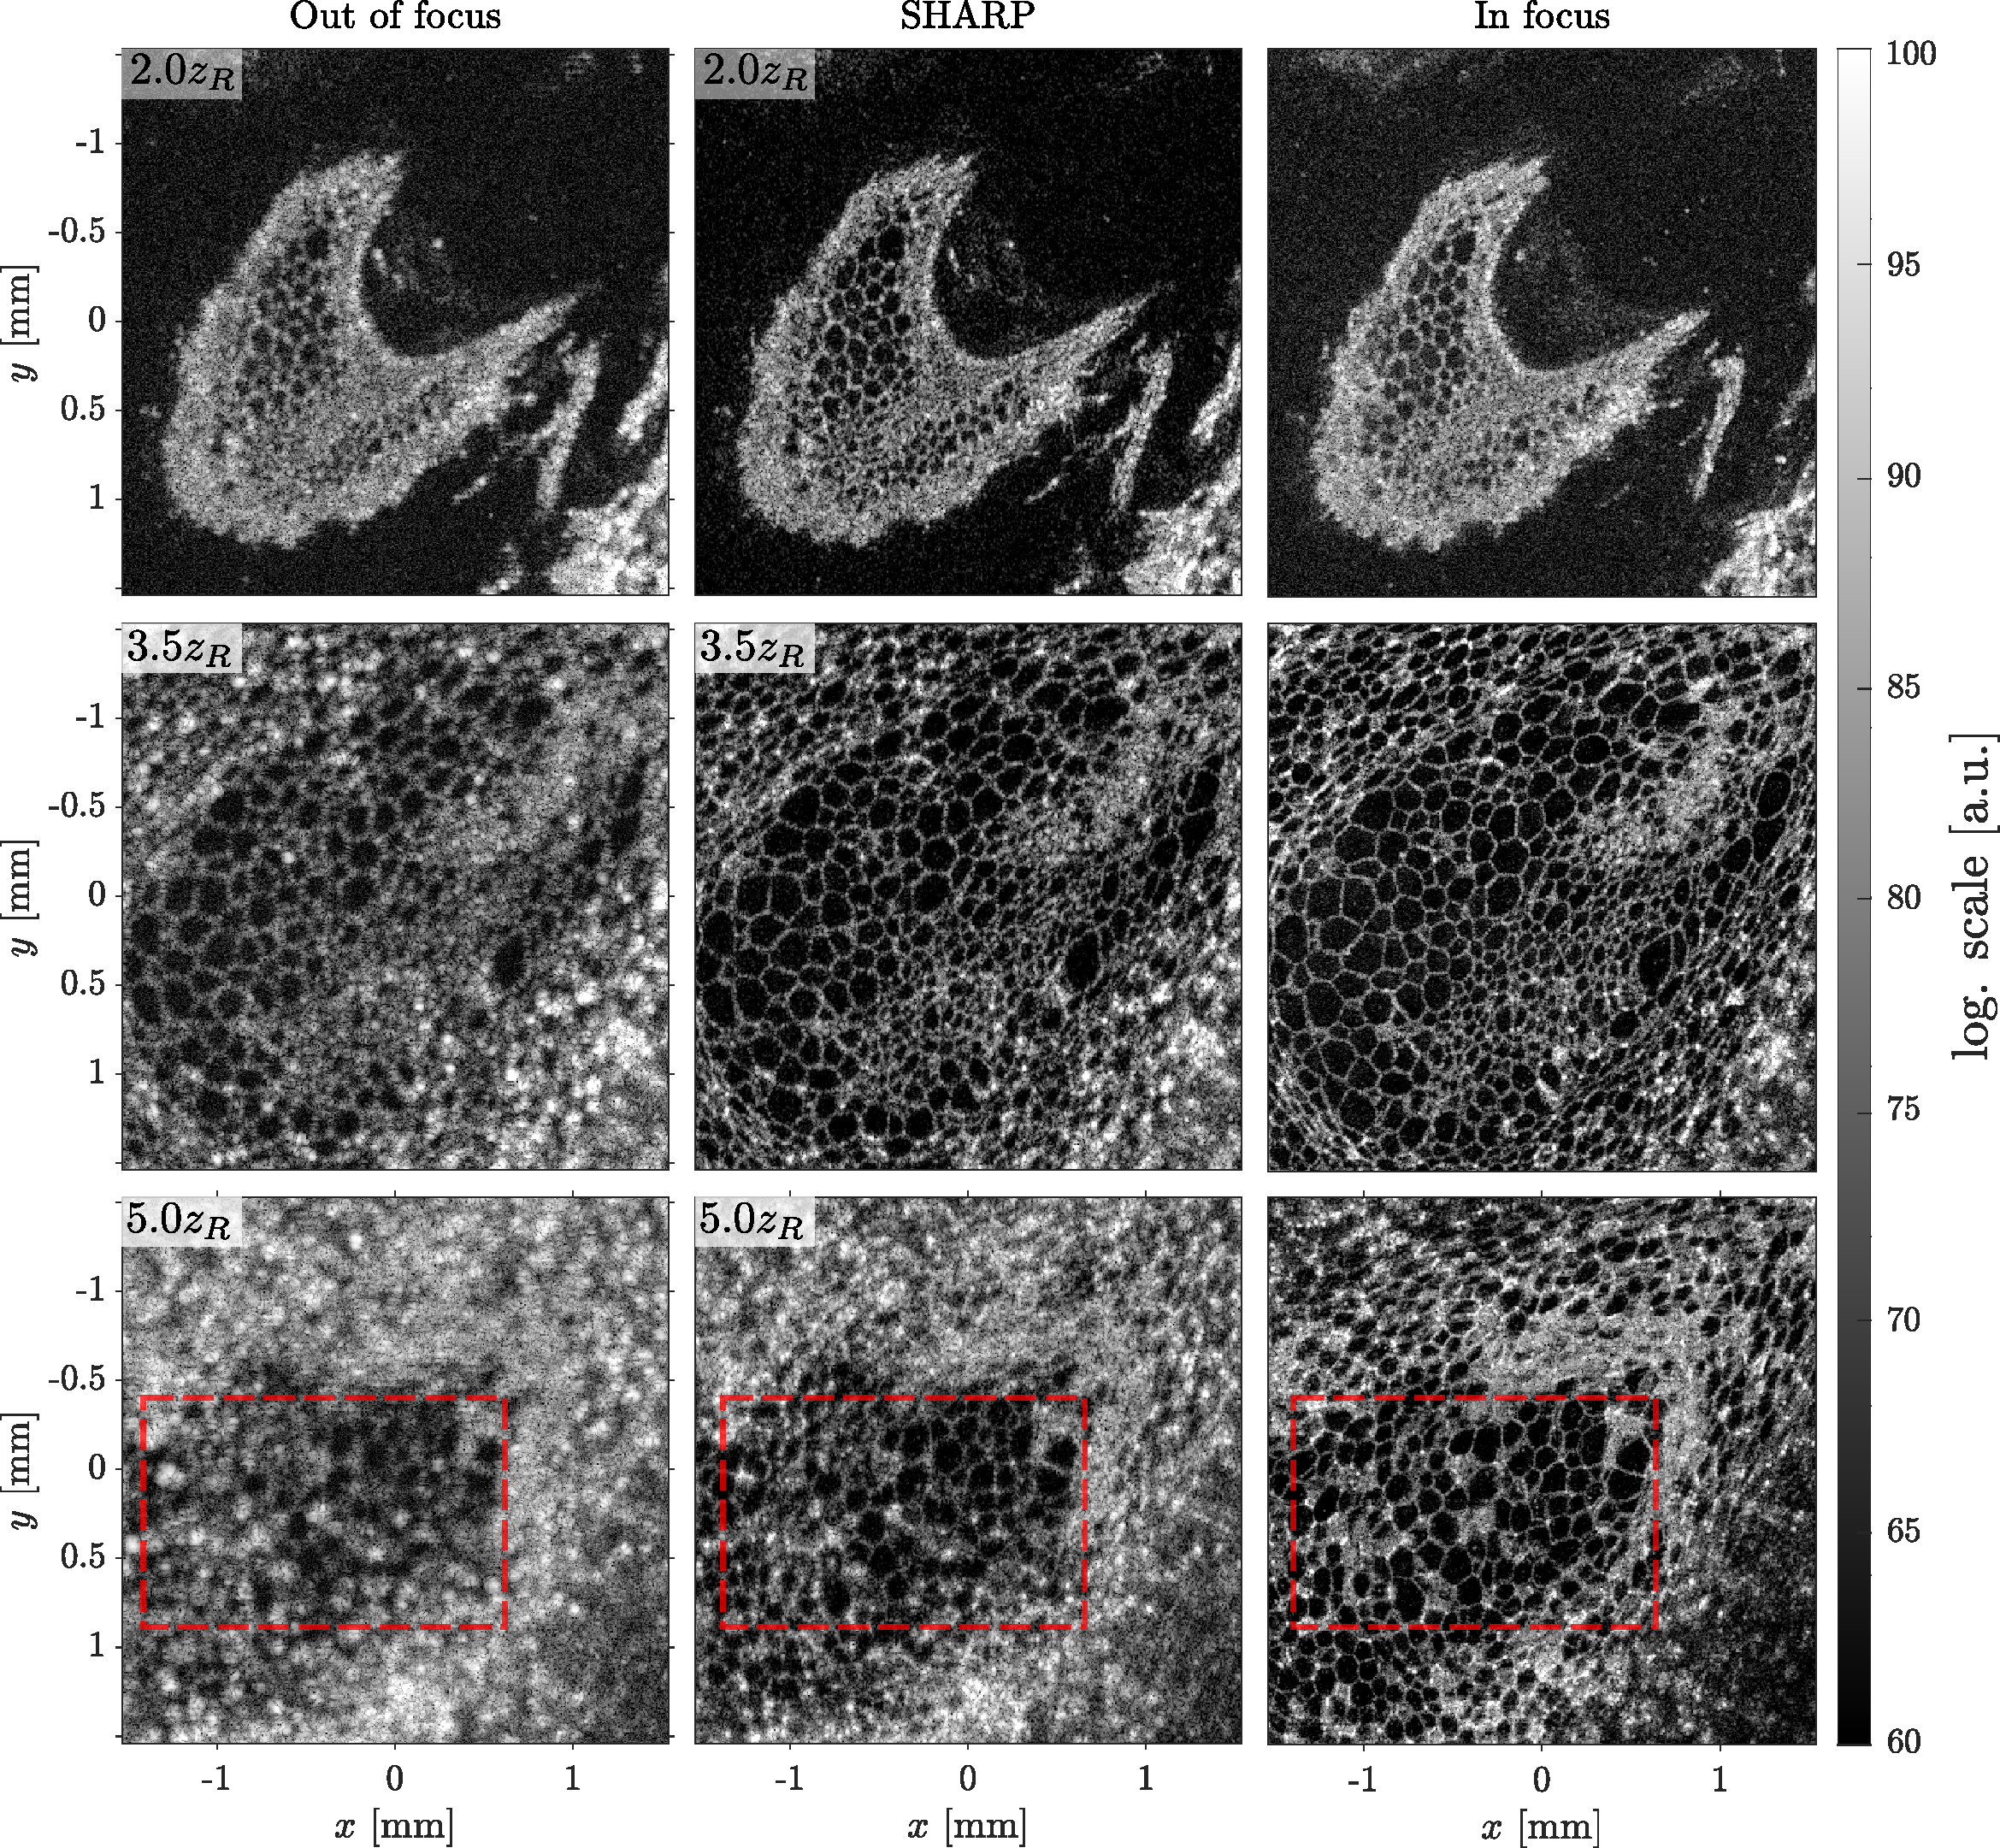
\includegraphics[width=\textwidth]{Figures/SHARP/SHARP_Cucumber_Enfaces.pdf}
	\caption[Comparison of several \textit{en face} views of out-of-focus, SHARP and in-focus tomograms.]{Comparison of several \textit{en face} views of out-of-focus, SHARP and in-focus tomograms, at depths $2.0z_R$, $3.5z_R$, and $5.0z_R$ as indicated in each image.}
	\label{fig:SHARP_CucumberEnfaces}
\end{figure}

Figure~\ref{fig:SHARP_CucumberEnfaces} presents \textit{en face} views located at depths $\sim 2.0z_R$, $3.5z_R$ and $5.0z_R$ from the focal plane of the OoF tomogram before and after SHARP, and of the corresponding in-focus reference tomogram. SHARP successfully restored the OoF tomogram despite the strong phase noise, providing images with better resolution and contrast than original images as a result of blurring correction and also due to the filtering effect of the optimum amplitude filter that reduced the average noise floor level from 63~dB to 59~dB, a difference corresponding to 1/10 of the images dynamic range 60--100~dB. In particular, cell walls of the sample are significantly sharper after SHARP compared to the original, approaching the in-focus counterparts, demonstrating the effectiveness of SHARP to correct for defocus.

For shallow depths, $2.0z_R$ and $3.5z_R$, SHARP produced successful results when compared to the reference images, but for the deepest plane shown, at $5.0z_R$, refocusing seems to be effective only for a small region having low signal density (see red boxes in Fig.~\ref{fig:SHARP_CucumberEnfaces}) whereas surrounding signal-dense region seems to be uncorrected. This may be a consequence of multiple scattering, which is likely to be stronger in these dense regions, and it is known that the deconvolution model only accounts for single-scattered or \textit{ballistic} photons, thus it is expected that a large contribution of multiple scattering hinders CAO, in this case for planes at $z>5.0z_R$ but this limit is sample-dependent.

SHARP was implemented in MATLAB and it took around 560~seconds to process the OoF tomogram in an ROI of size 450$\times$512$\times$512, using MATLAB 2019a in a workstation computer running on an Intel core i7-8700 processor @~3.2GHz. Aberration correction steps are the most computational expensive because of the optimization procedure performed in CAO, taking around 528 seconds for all planes including the two 1D corrections. In practical scenarios, it is possible to run the optimization only for certain planes and then to fit the optimal weights to find the correction for the intermediate planes, given that evolution of aberrations over depth is indeed smooth, and this will effectively reduce computation time.

\FloatBarrier

\section{Extending SHARP}\label{sec:Extensions}

\subsection{Complex amplitude motion artifacts correction}\label{sec:MotionCor}

Relevant effects of motion in the OCT signal for the context of CAC were already explain in Section~\ref{sec:phaseStab}, namely complex amplitude shift and phase-jump. The latter often has a greater relevance for CAC, thus phase stabilization methods correct phase offsets, including the phase stabilization performed in SHARP. However, in many \textit{in vivo} applications, complex amplitude shift may also have a significant influence and could be more noticeable since they affect both the phase and the amplitude of the tomogram, appearing as signal distortions in the structural image~\cite{Kraus2015_OCT}. In general, OCT systems are equipped with sample holders or interfaces to reduce impact of large acute motion, for instance chin rests and forehead holders in ophthalmic systems or handheld scanners for skin imaging, but there is yet low-frequency, slow motion arising from the heartbeat and respiration of the subject~\cite{Kraus2015_OCT}.

Motion artifacts can be prevented or corrected using a reference motion-free image from other imaging modality~\cite{Ricco2009_Correcting}, using tracking systems that follow and correct for sample motion \textit{in situ}, employed specially in retinal imaging~\cite{Maguluri2007_Three}, or using fast systems with volume acquisition rate such that sample appears static during the scanning, for instance recent reports have achieved volume acquisition rates in the order of tents of milliseconds with A-lines rates of the order of MHz~\cite{Auksorius2020_vivo}, but employing very specialized components. With A-line acquisition rates of the order of 100~kHz in current widespread systems, it is possible to assume that, in normal conditions, the sample is static during the acquisition of a single B-scan and motion manifests as rigid-body displacements across different B-scans, in other words, as inter-B-scan bulk displacements. In such case, complex amplitude shifts can be corrected straightforwardly using image registration~\cite{Zawadzki2007_Correction}.

The idea of bulk image registration is to find the relative global shift between two given images $I_1(m,l)$ and $I_2(m,l)$~\cite{Guizar-Sicairos2008_Efficient}. Most used method is intensity-based registration where the cross-correlation $r_{\text{cc}} = I_1(m,l)\star I_2(m,l)$ of the two images is computed and the location of the peak is found to determined the relative shift $(m_{\text{cc}}, l_{\text{cc}})$ between the two images, assuming that they are almost identical except for the relative shift between them. Then, the shift is applied to one of the two images in order to match one to the other. Commonly, cross-correlation is computed in Fourier domain as 
\begin{equation}\label{eq:ImageReg}
    r_{\text{cc}} = \text{FT}^{-1}_{q_m,q_l}\left\{\text{FT}_{m,l}\left\{I_1(m,l)\right\}\text{FT}_{m,l}\left\{I_2(m,l)\right\}^\ast\right\},
\end{equation}
where $^\ast$ denotes complex conjugate, then the shift is corrected as
\begin{equation}
    I_2 = \text{FT}^{-1}_{q_m,q_l}\left\{\text{FT}_{m,l}\left\{I_2(m,l)\right\} \exp\left[-i2\pi\left(m_{\text{cc}} \frac{q_m}{M} + l_{\text{cc}} \frac{q_l}{L}\right)\right]\right\},
\end{equation}
where $m_{\text{cc}}$ and $l_{\text{cc}}$ are given in pixels and $M\times L$ is the image size.

When a sub-pixel estimation is required, the product of the two Fourier-transformed images in Eq.~\eqref{eq:ImageReg} is zero-padded prior to computation of the inverse FT in order to have an upsampled cross-correlation $r_{\text{cc}}$. However, this zero-padding will increase the size of the input of the inverse FT increasing computational cost significantly as the sub-pixel resolution increases, for instance a $1/20$ resolution requires a zero-padding of $20M\times 20L$. Fortunately, there are efficient sub-pixel image registration methods that significantly improve speed without sacrificing accuracy~\cite{Guizar-Sicairos2008_Efficient}.

Using efficient sub-pixel image registration, it is possible to include a step for inter-B-scan bulk motion correction in SHARP procedure, assuming that transitions between B-scans is smooth, which is valid for typical biological samples scanned with a proper sampling, ideally equal or better than Nyquist sampling. This step, if necessary, is performed after the first phase stabilization step since correcting the complex signal requires phase stable data. Complex-shifts correction could enable operation of subsequent steps of SHARP for \textit{in vivo} imaging. Motion is corrected in SHARP by registering intensity of adjacent B-scans $n$ and $n-1$ and finding the relative lateral and axial shifts $(m_\text{cc}(n), l_\text{cc}(n))$ as
\begin{equation}
    (m_\text{cc}(n), l_\text{cc}(n)) = \arg\left\{\max\left\{ |S(m,n,l)|^2\star |S(m,n-1,l)|^2 \right\}\right\},
\end{equation}
where the cross-correlation is performed inside the B-scan plane, i.e. along coordinates $x$ and $z$. Shifts across B-scans are accumulated to computed global shifts with respect to the first B-scan as
\begin{equation}
    \mu_{\text{cc}}(n) = \sum_{\hat{n}}^n m_{\text{cc}}(\hat{n}) \ \ \ \ \ \text{and} \ \ \ \ \  \Gamma_{\text{cc}}(n) = \sum_{\hat{n}}^n l_{\text{cc}}(\hat{n}),
\end{equation}
that are applied to obtain a bulk motion-corrected complex tomogram $S_\text{mc}(m,n,l)$,
\begin{equation}
    S_\text{mc}(m,n,l) = \text{FT}^{-1}_{q_m,q_l}\left\{\text{FT}_{m,l}\left\{S(m,n,l)\right\} \exp\left[-i2\pi\left( \mu_{\text{cc}}(n)\frac{q_m}{M} + \Gamma_{\text{cc}}(n)\frac{q_l}{L}\right)\right]\right\}.
\end{equation}

Additionally, global shifts can be high-pass filtered to cancel out the spurious low-frequency shifts that appear when the sample has a non-flat geometry, for instance the curvature of the cornea, in order to preserv the surface geometry of the sample.

With this motion correction step, it could be possible to correct $x$-$y$-separable aberrations with SHARP in tomograms acquired \textit{in vivo} affected by bulk motion subject to the B-scan plane (inter-B-scan), but insignificant out-of-plane motion (intra-B-scan) since it is not addressed in the approach described above, actually out-of-plane corrections demands more sophisticated solutions out of the scope here~\cite{Kraus2012_Motion}. To register B-scans, the efficient sub-pixel image registration by cross-correlation algorithm~\cite{Guizar-Sicairos2008_Efficient} is used here, available in \href{https://www.mathworks.com/matlabcentral/fileexchange/18401-efficient-subpixel-image-registration-by-cross-correlation}{MATLAB Central File Exchange}~\cite{Guizar2020_Efficient}.

Figure~\ref{fig:MotionCor} illustrates motion correction with the simulated OCT tomogram used in previous demonstrations. Global lateral and axial shifts were defined randomly for each B-scan and applied to the original motion-free tomogram, then the motion correction procedure was carried out to compensate for the induced shifts using a sub-pixel resolution of $1/20$. Figs.~\ref{fig:MotionCor}(a)-(c) compare \textit{en face} views of each tomogram, and the effect of inter-B-scan bulk motion can be visualized in Fig.~\ref{fig:MotionCor}(b) as distortions and discontinuities along the $y$ axis. This is also evident comparing the cross-sectional $z$-$y$ planes in Figs.~\ref{fig:MotionCor}(d)-(f). In both views, it is clear that the motion correction yields a tomogram with no perceptual artifacts, approaching the appearance of the original one. In Fig.~\ref{fig:MotionCor}(g), a zoomed region of the cross-correlation image between two B-scan with relative shift of 3 pixels is shown, to illustrate how the location of the peak is shifted from the center of the image, indicating the relative displacement. 

\begin{figure}[htb!]
	\centering
	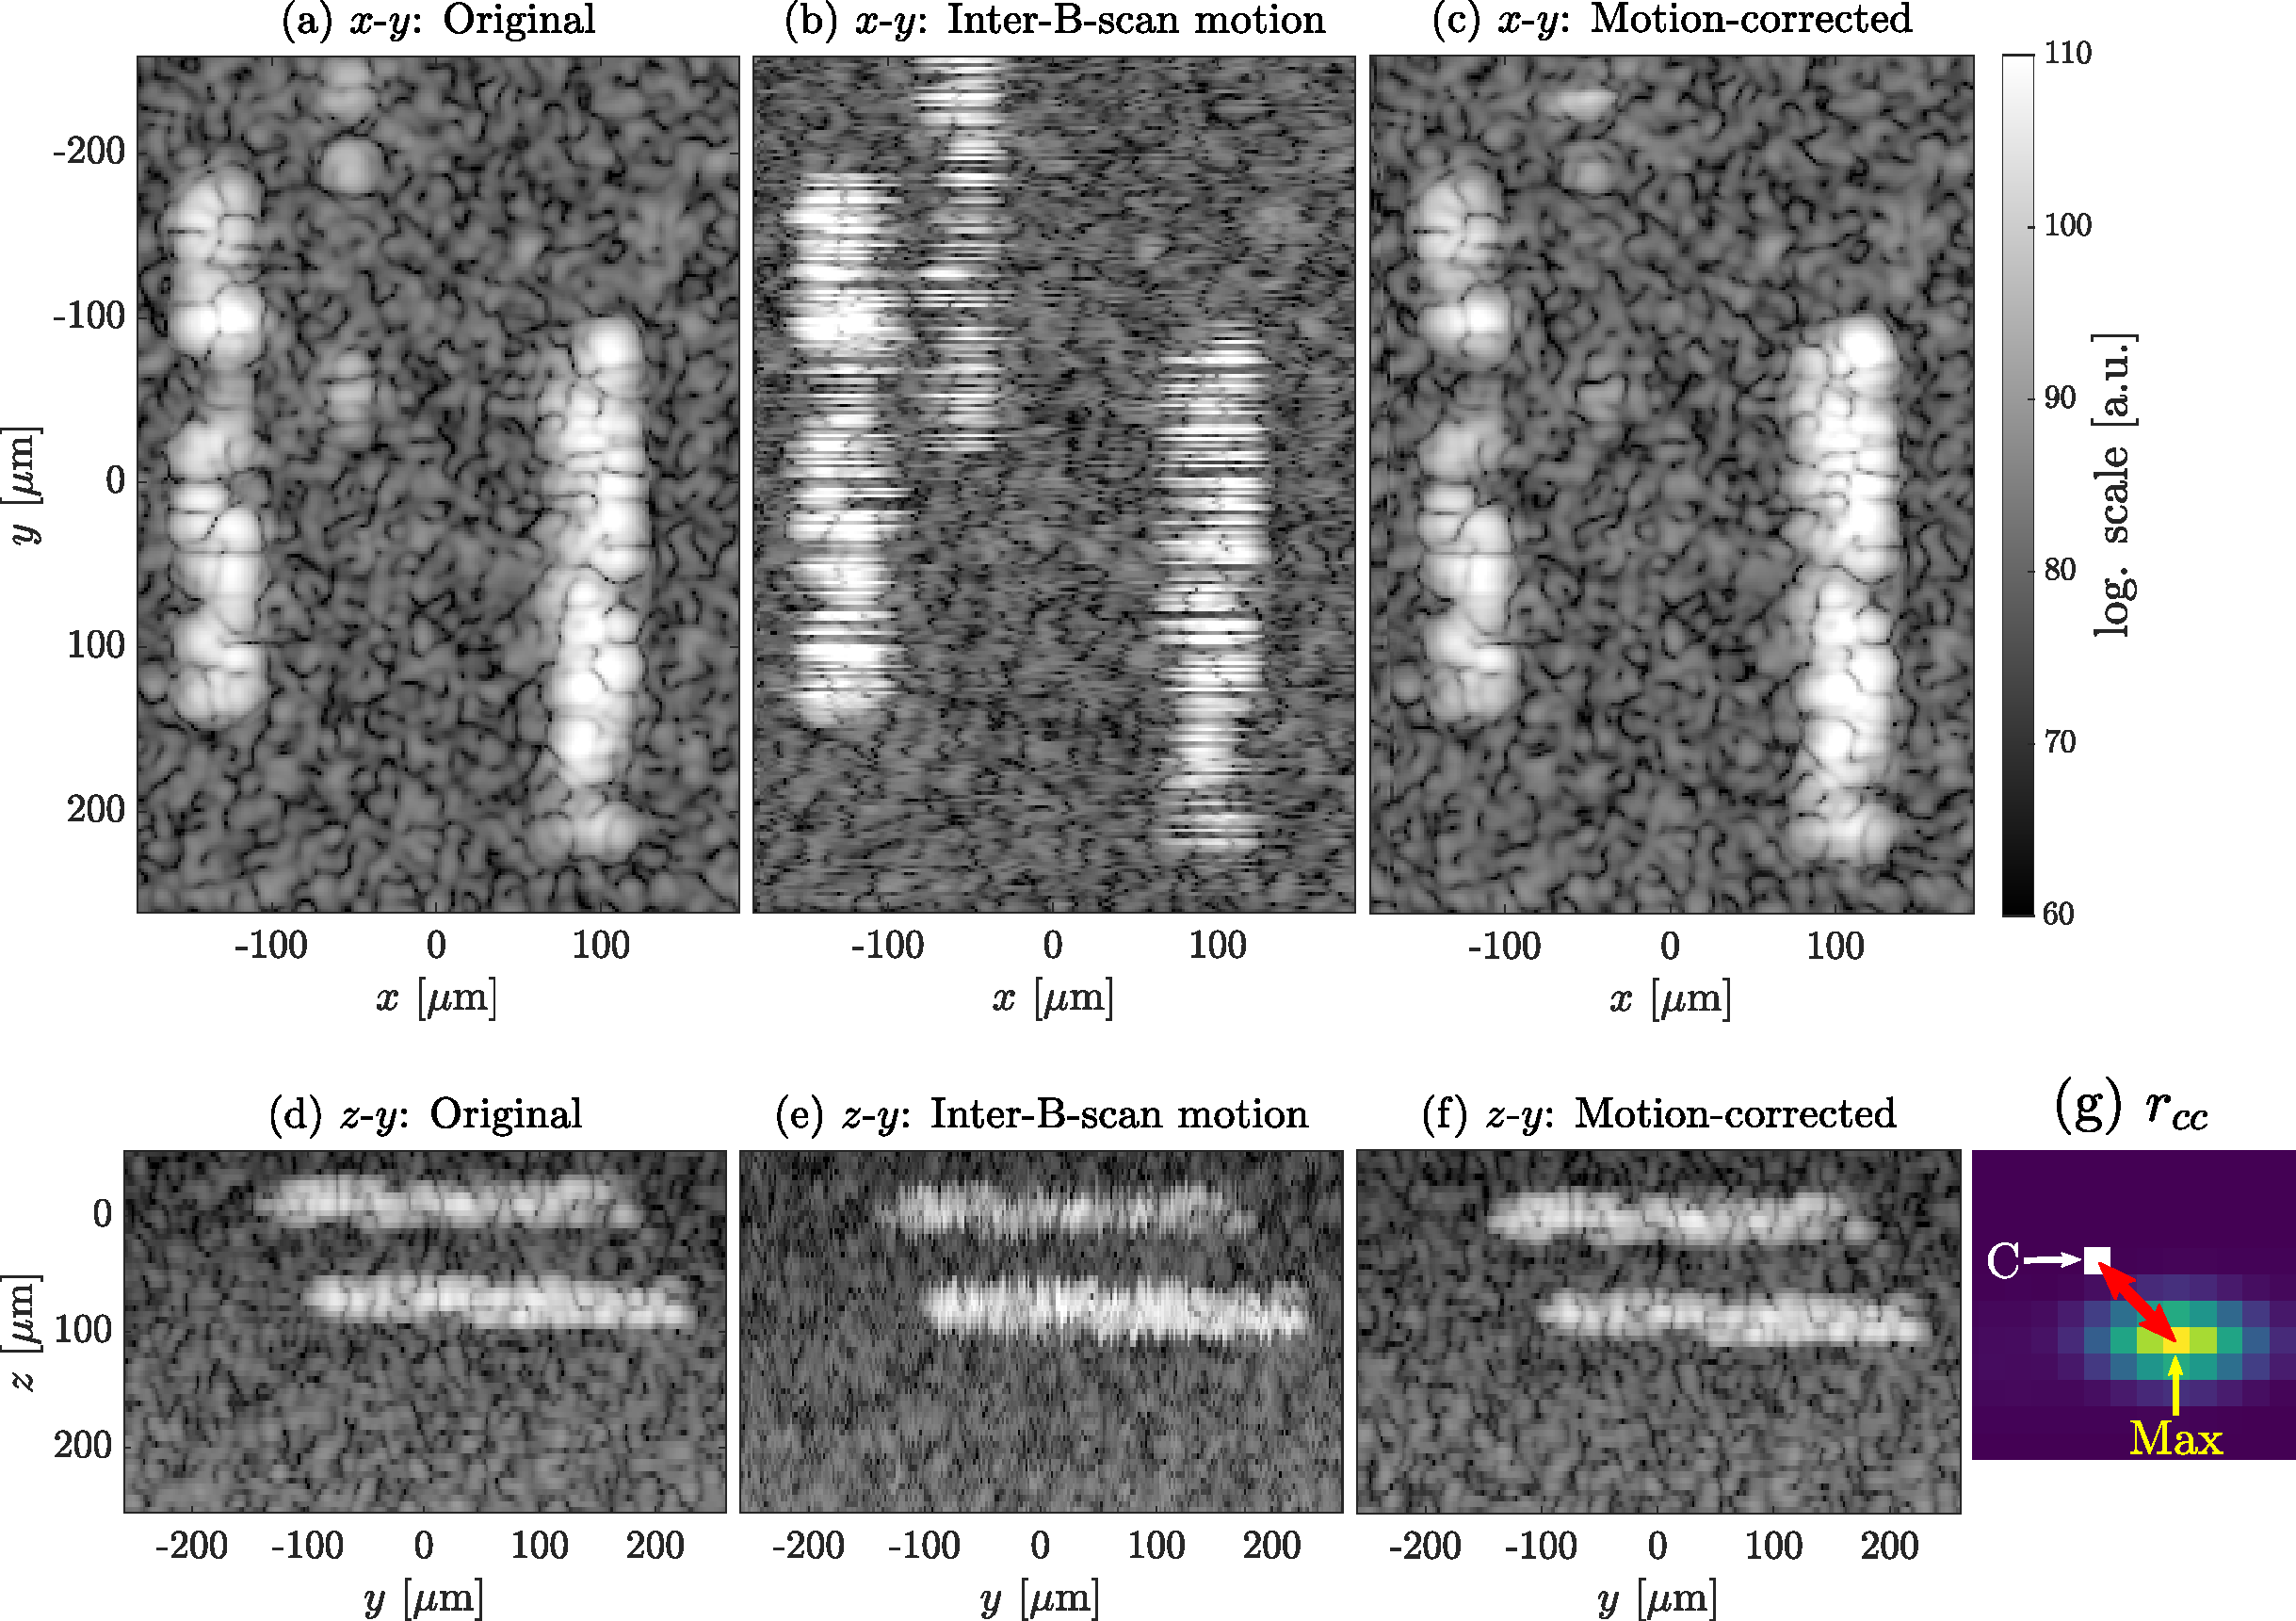
\includegraphics[width=\textwidth]{Figures/SHARP/MotionCorrection.pdf}
	\caption[Illustration of intra-B-scan motion correction with a simulated OCT tomogram.]{Illustration of intra-B-scan motion correction with a simulated OCT tomogram. (a), (d) original; (b), (e) original with induced axial and lateral in-plane bulk motion; (c), (f) motion corrected using image registration. (a)-(c) are \text{en-face} views and (d)-(f) are cross-sections of $z$-$y$ plane. (g) Example of the cross-correlation between two B-scan with relative motion (not shown). C: center pixel, Max: location of the maximum value of the cross-correlation. Red arrow indicates the estimated shift between the two B-scans.}
	\label{fig:MotionCor}
\end{figure}
\FloatBarrier

\subsection{Spatially-varying aberrations correction}

Although the numerical deconvolution in CAO is performed in Fourier domain for practical simplicity, by applying a complex filter to each \textit{en face} plane, the physical convolution in the image formation process actually occurs in spatial domain. The possibility to perform the numerical deconvolution in Fourier domain relies on the fact that the deconvolution kernel in spatial domain is constant over the lateral field of view (FoV) ---not to be confused with axial depth of field.--- The region within this assumption is valid is known as the \textit{isoplanatic-patch}, a term originated from astronomy~\cite{Beckers1993_Adaptive}, defined as the region within which aberrations and therefore the point spread function (PSF) do not vary~\cite{Kumar2015_Anisotropic}. There are scenarios where the lateral FoV is greater than the isoplanatic-patch, consequently the PSF is anisotropic resulting in aberrations that vary across the FoV thus they cannot be corrected entirely using a global filter in Fourier domain.  For instance, it is known that large numerical aperture systems often have a small diffraction-limited lateral FoV and outside this the resolution degrades progressively. Additional causes of an anisotropic PSF may be imperfect optical components, misalignment, or inhomogeneous samples, for instance in corneal imaging, where the axial focal position is not longer constant forming a plane, instead it is curved as a consequence of cornea curvature.

In rigorous terms, spatial-varying aberrations must be corrected locally, using a deconvolution kernel defined individually at each spatial coordinate. This would be computationally expensive and a fully localized correction might not be necessary for certain practical scenarios because variation of aberrations across the FoV is indeed smooth. To deal with spatial-varying aberration, region of interest-based CAO have been proposed for sub-aperture-based and optimization-based CAO~\cite{Kumar2015_Anisotropic, South2019_Local} under the general idea of splitting the FoV into several regions of interests (ROIs) or windows to perform CAO individually in each ROI and then stitching the aberration-corrected ROIs into the original full FoV. Ideally, aberrations within each ROI should be nearly constant, this is achievable using small ROIs, but in practice there is a limit on the minimum size given that the determination of aberrations in the CAO procedure could fail if few pixels are used.

Based on former idea, it is possible to perform spatially-varying aberration correction in SHARP procedure, as is illustrated in Figure~\ref{fig:spatialAber}, instead of using the standard global aberration correction. To do so, each \textit{en face} plane is splitted into windows of size $W_x\times W_y$ with an overlap of half window size along the axis being corrected, for instance, an overlap of $W_x/2\times 0$ when correcting in $x$ axis, or $0\times W_y/2$ for $y$ axis. Given the 1D operation of SHARP, overlap is not necessary in the axis that is not the interest in each aberration-correction step. The purpose of overlapping the windows is to avoid boundaries artifacts that appear in the composite images when there is not overlap. After performing CAO in each window, full \textit{en face} planes are assembled extracting an centered ROI of size $W_x/2\times W_y$  from each window when correcting along $x$, or $W_x\times W_y/2$ when correcting along $y$ axis. For windows occupying the frontier of the full image in the axis of interest (red box in Fig.~\ref{fig:spatialAber}), an extended ROI is selected in order to keep the same full image size. The appropriate number of windows may change for every tomogram depending on the sample and the anisotropy of aberrations.

\begin{figure}[htb!]
	\centering
	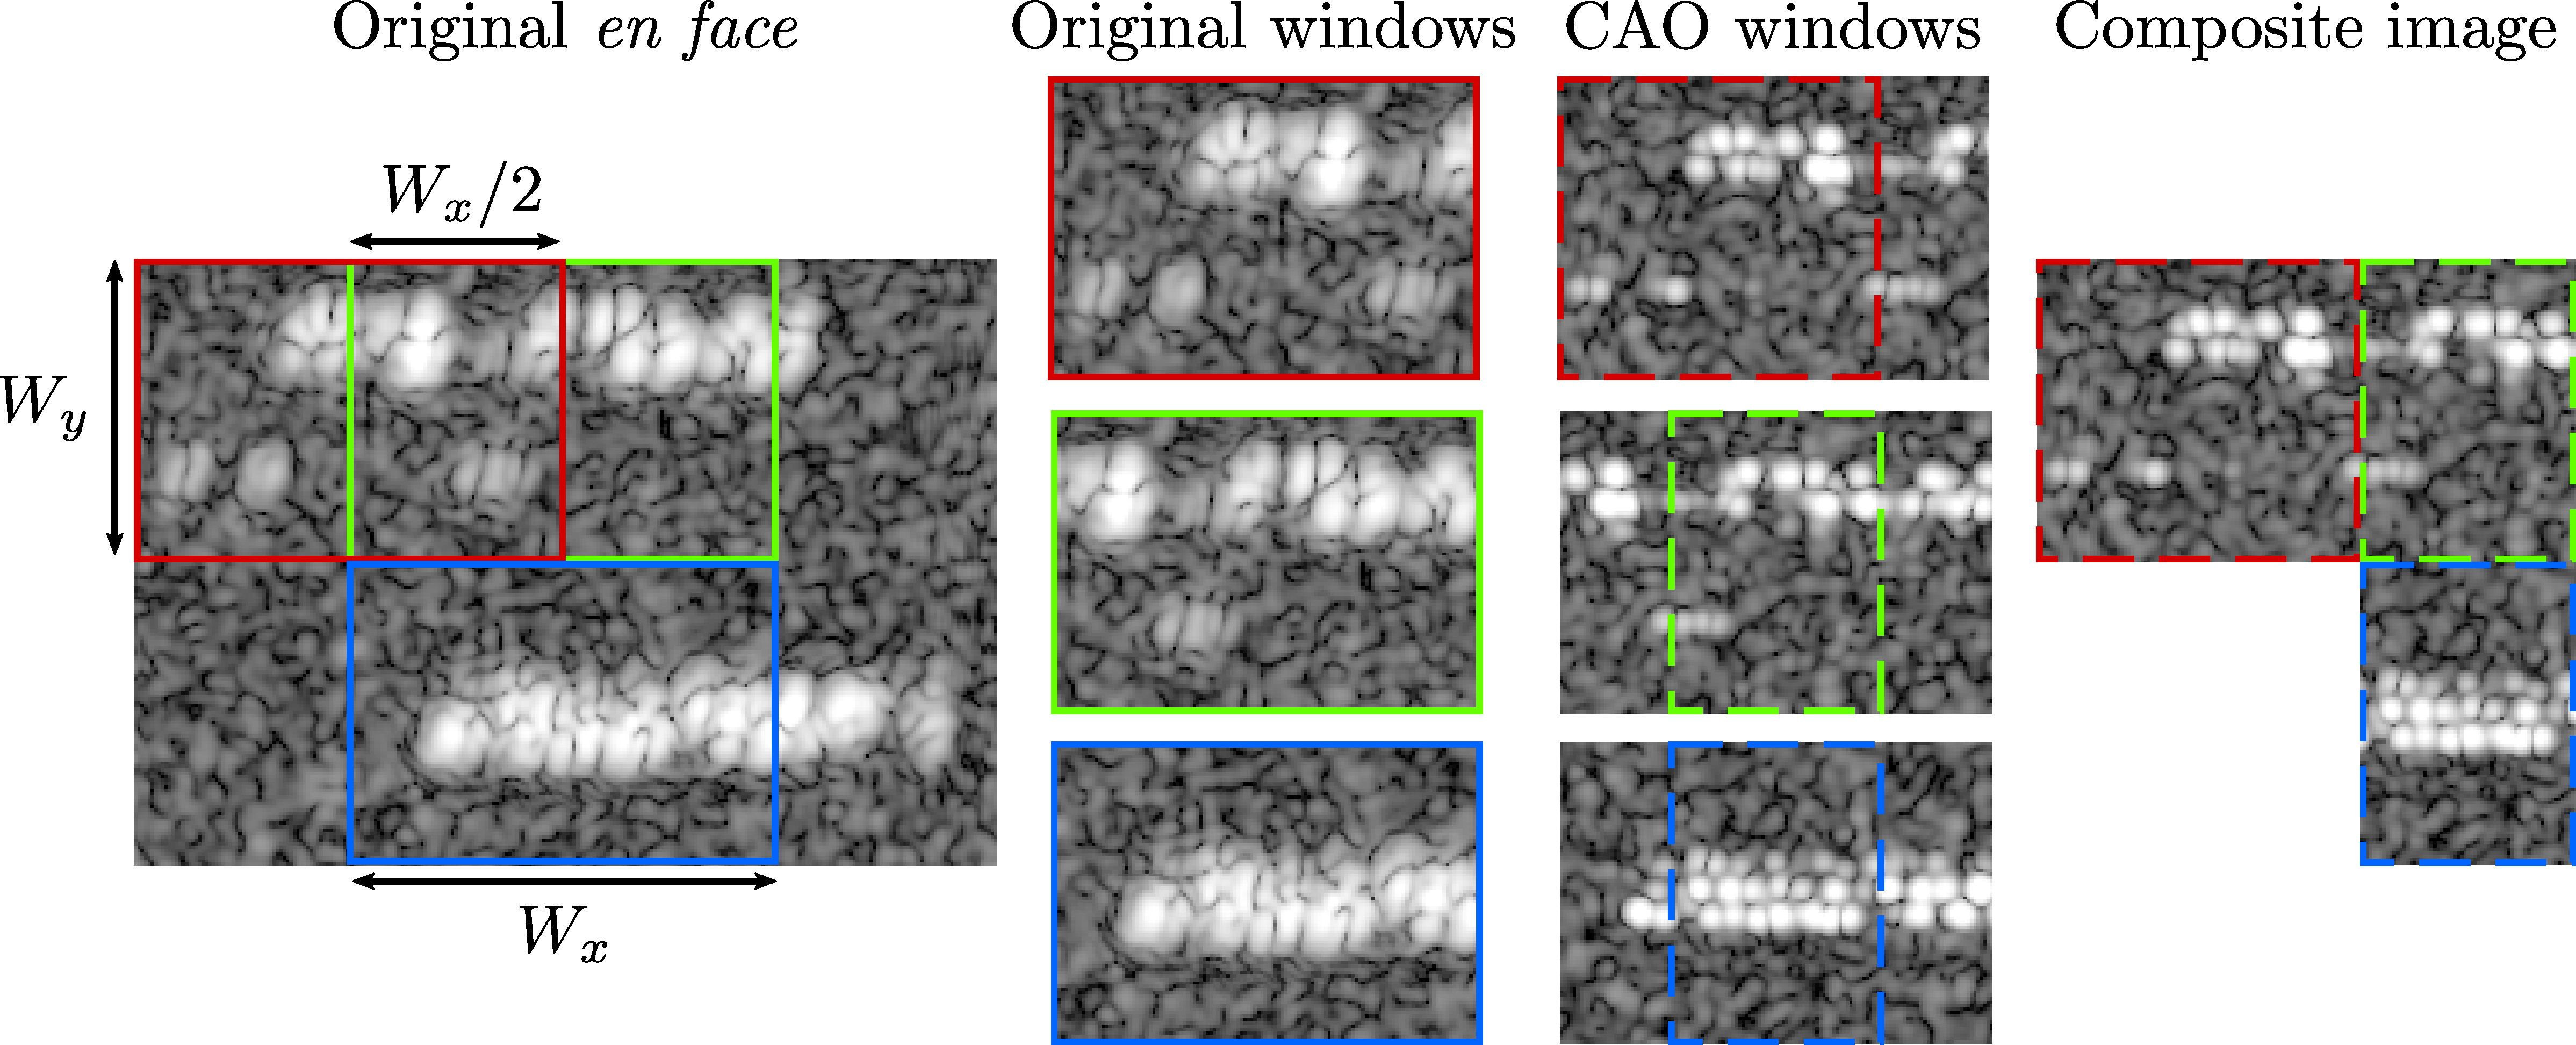
\includegraphics[width=\textwidth]{Figures/SHARP/SpatialVarAber.pdf}
	\caption[Illustration of spatially-varying aberration correction with a simulated OCT \textit{en face}.]{Illustration of spatially-varying aberration correction with a simulated OCT \textit{en face}, showing the process for three windows only to facilitate interpretation.}
	\label{fig:spatialAber}
\end{figure}


\FloatBarrier

\subsection[Beyond correction of separable in \textit{x-y} aberrations]{Beyond correction of separable in $x$-$y$ aberrations}

Although SHARP is capable of correcting for defocus and $xy$-astigmatism, the two major aberrations in OCT for many applications, a clear drawback is the constrain to only correct for $x$-$y$-separable aberrations, and this could limit applicability of SHARP, in particular, in retinal imaging applications given that arbitrary aberrations are present depending on the subject's eye~\cite{Kumar2017_Invivo, Ginner2018_Holographic, Hillmann2016_Aberrationfree}, It is therefore desirable to extend the procedure to cover more general aberrations and expand its applicability throughout more practical scenarios.

In the standard or SHARP-$xy$ procedure, aberrations are corrected along the two main axes $x$ and $y$. Keeping in mind the 1D operation, it is possible to correct aberrations along two secondary axes $x'$ and $y'$ obtained as the original axes $x$ and $y$ rotated by 45 degrees with the relationships $x'=x\cos45^\circ - y\sin45^\circ$ and $y' = x\sin45^\circ + y\cos45^\circ$. In principle, correcting for aberrations in the axes $x$-$y$ and then in the axes $x'$-$y'$ provides a global correction of aberrations oriented at an arbitrary angle. For instance, SHARP-$xy$ and SHARP-$x'y'$ can correct for $xy$- and oblique-astigmatism respectively, then complementing both procedures, it is possible to correct for astigmatism oriented at an arbitrary angle obtained from a combination of the two independent astigmatisms. 

The procedure for SHARP-$x'y'$ follows the idea behind the simple steps of the original method with slight differences as explain next and illustrated in Figure~\ref{fig:SHARP45d_Diag} for a grid of $6\times 6$ pixels. Local phase differences $\delta(m,n)$ for phase noise correction are computed between consecutive A-lines oriented in oblique paths [red lines in Fig.~\ref{fig:SHARP45d_Diag}(b)], denoted by indexes $(m,n)$ and $(m-1, n+1)$ in the case of correcting along $x'$ axis or $(m,n)$ and $(m+1, n-1)$ when correcting along $y'$ axis, then the proper accumulative sum is performed and this way phase stability is achievable along any oblique axis, $x'$ or $y'$. After phase stabilization, it is now possible to perform aberration correction along the phase-stable oblique axis.

\begin{figure}[htb!]
	\centering
	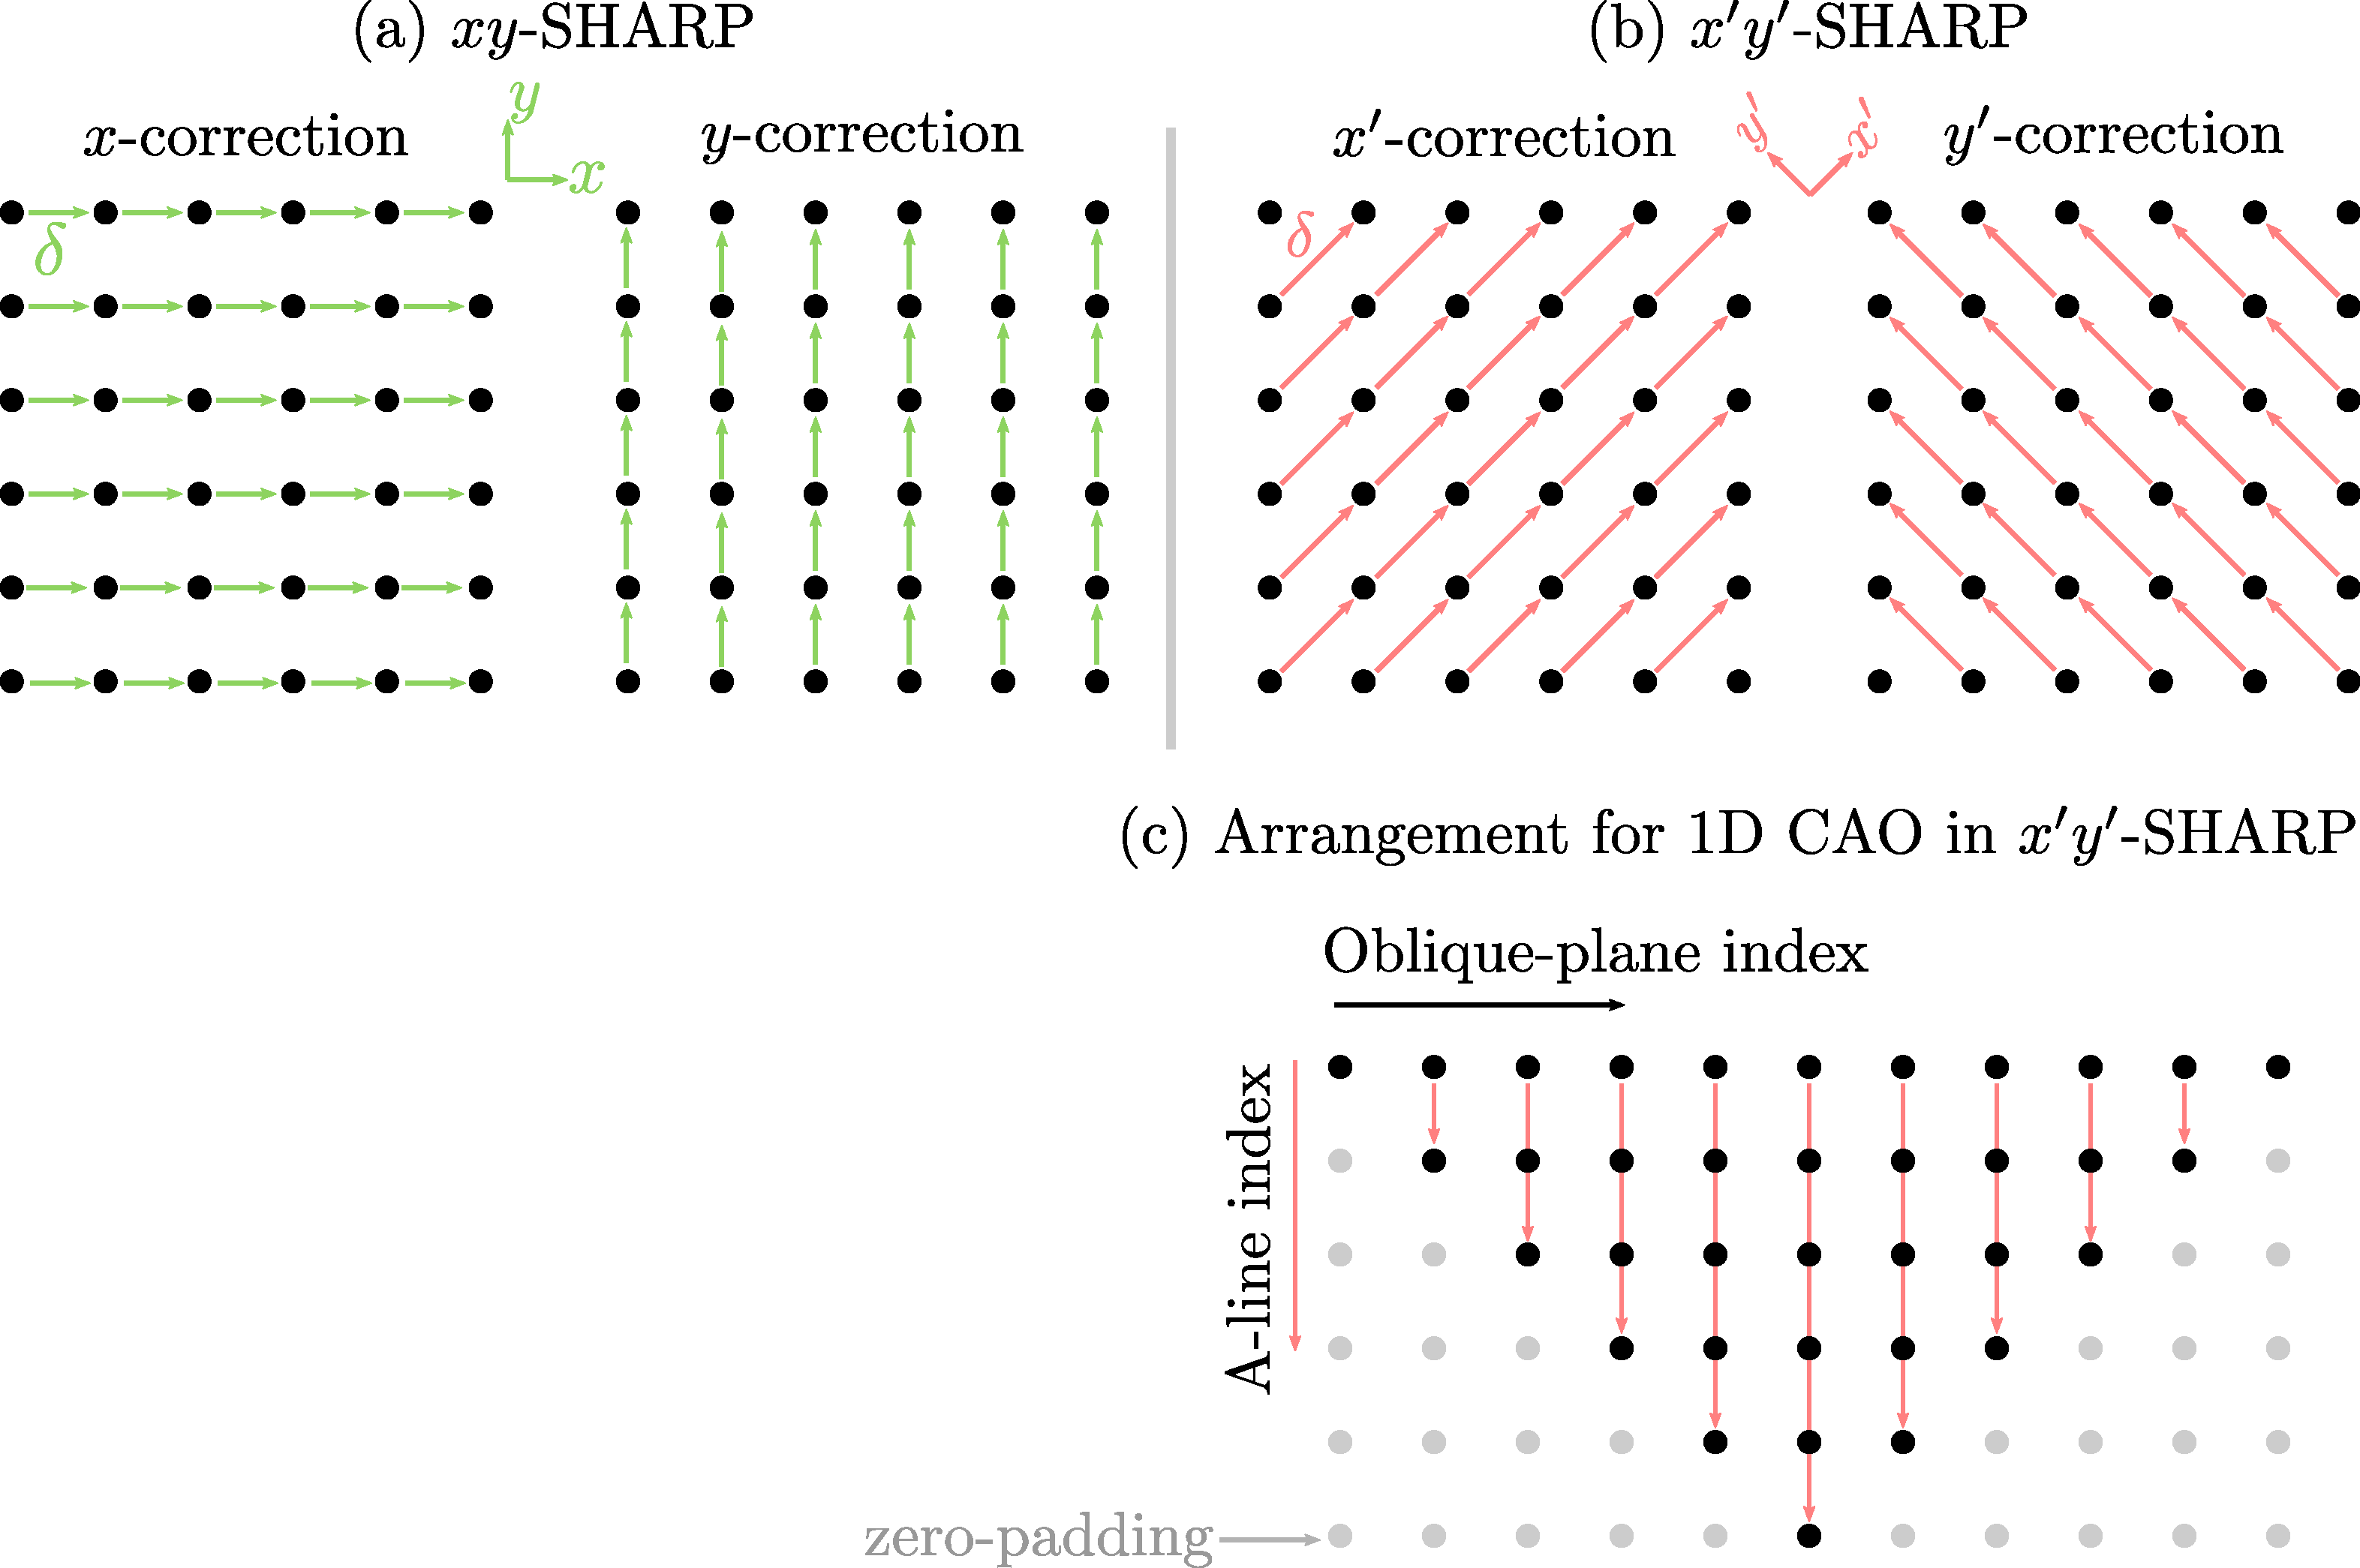
\includegraphics[width=\textwidth]{Figures/SHARP/SHARP45d_Diagram.pdf}
	\caption[Comparison of operation of SHARP-$xy$ and SHARP-$x'y'$.]{Comparison of operation of SHARP-$xy$ and SHARP-$x'y'$ for a grid of $6\times 6$ pixels. (a) Phase differences in SHARP-$xy$ are computed along vertical and horizontal paths, whereas (b) for SHARP-$x'y'$ are computed along oblique paths. (c) The tomogram grid is rearranged in order to perform CAO along an oblique axes.}
	\label{fig:SHARP45d_Diag}
\end{figure}

The essence of 1D CAO for the oblique axes is the same as that for the main axes but there are changes in the numerical implementation in order to carry out the corresponding calculations.  In a standard tomogram, \textit{en face} plane is arranged with one dimension being A-line index ($x$ axis) and the other being B-scan plane index ($y$ axis). To carry out 1D CAO in SHARP-$x'y'$, the tomogram is rearranged in the \textit{en face} plane in such way that one dimension corresponds to the A-line index ($x'$ axis) and the other to the oblique-plane index ($y'$ axis) [see Fig,~\ref{fig:SHARP45d_Diag}(c)]. In addition, the rearranged tomogram is zero-padded to keep a constant oblique-plane size because original planes have different numbers of A-lines. Then, the standard 1D CAO procedure can be applied directly to the rearranged tomogram using the A-line index dimension as the aimed dimension for the calculations.

The zero-padding in the rearrangement step provides a tomogram with uniform size, but it is clear that the number of A-lines with effective (non-zero) information in each oblique-plane is different, and it approaches to one A-line towards the tomogram frontiers. Because of that, planes having less A-lines than the deconvolution kernel size will possibly end up with a wrong correction, however, this effect is unimportant given that it occurs only towards the corners  of the FoV.

Because phase differences for noise correction in SHARP-$x'y'$ are computed between A-lines separated by $\sqrt{2}$ times the lateral sampling (and not by exactly the lateral sampling as in SHARP-$xy$), then in order to fulfill sampling requirement for CAO, the effective sampling of the tomogram should be $1/\sqrt{2}$ times the Nyquist sampling, i.e. $\delta_x/(2\sqrt{2})$, or smaller, this means that a finer lateral sampling is required. This is a key aspect to keep in mind but it does not have important experimental consequences given that in most systems sampling can be adjusted.

In the case of performing SHARP-$x'y'$ after applying SHARP-$xy$, it is important to rollback the last phase noise correction after the second aberration correction of  SHARP-$xy$, otherwise, subsequent phase noise corrections are likely to fail. In general, the entire SHARP procedure would consist in four steps, each one performing a phase noise and aberration correction along a single axis at a time, connected by their corresponding rollback step. An intuitive order for the axis of interest is each step is first $x$, then $y$, then $x'$ and finally $y'$, although order can be changed indistinctly.

A preliminary test using the simulated OCT tomogram mentioned previously was carried out to verify the correct operation of SHARP-$x'y'$ and results are summarized in Fig.~\ref{fig:SHARP45d_Int}. To establish a reference for comparison, intrinsic defocus of the tomogram was corrected using 2D CAO. Aberrations were induced in the original tomogram by applying a phase filter created with Zernike polynomials $Z_4$ and $Z_5$ for $xy$- and oblique-astigmatism with weights $0.8\lambda$ and $2.4\lambda$ respectively. Figs.~\ref{fig:SHARP45d_Int}(a) and (b) show one \textit{en face} plane of the aberration-free and aberrated tomograms. Fig.~\ref{fig:SHARP45d_Int}(e) shows the aberration wavefront exhibiting astigmatism oriented at an arbitrary angle, but close to 45 degrees given that the magnitude of the weight of $Z_5$ is greater, and it also shows the aberrated wavefront for the \textit{en face} plane Figs.~\ref{fig:SHARP45d_Int}(b) including its intrinsic defocus. 

\begin{figure}[htb!]
	\centering
	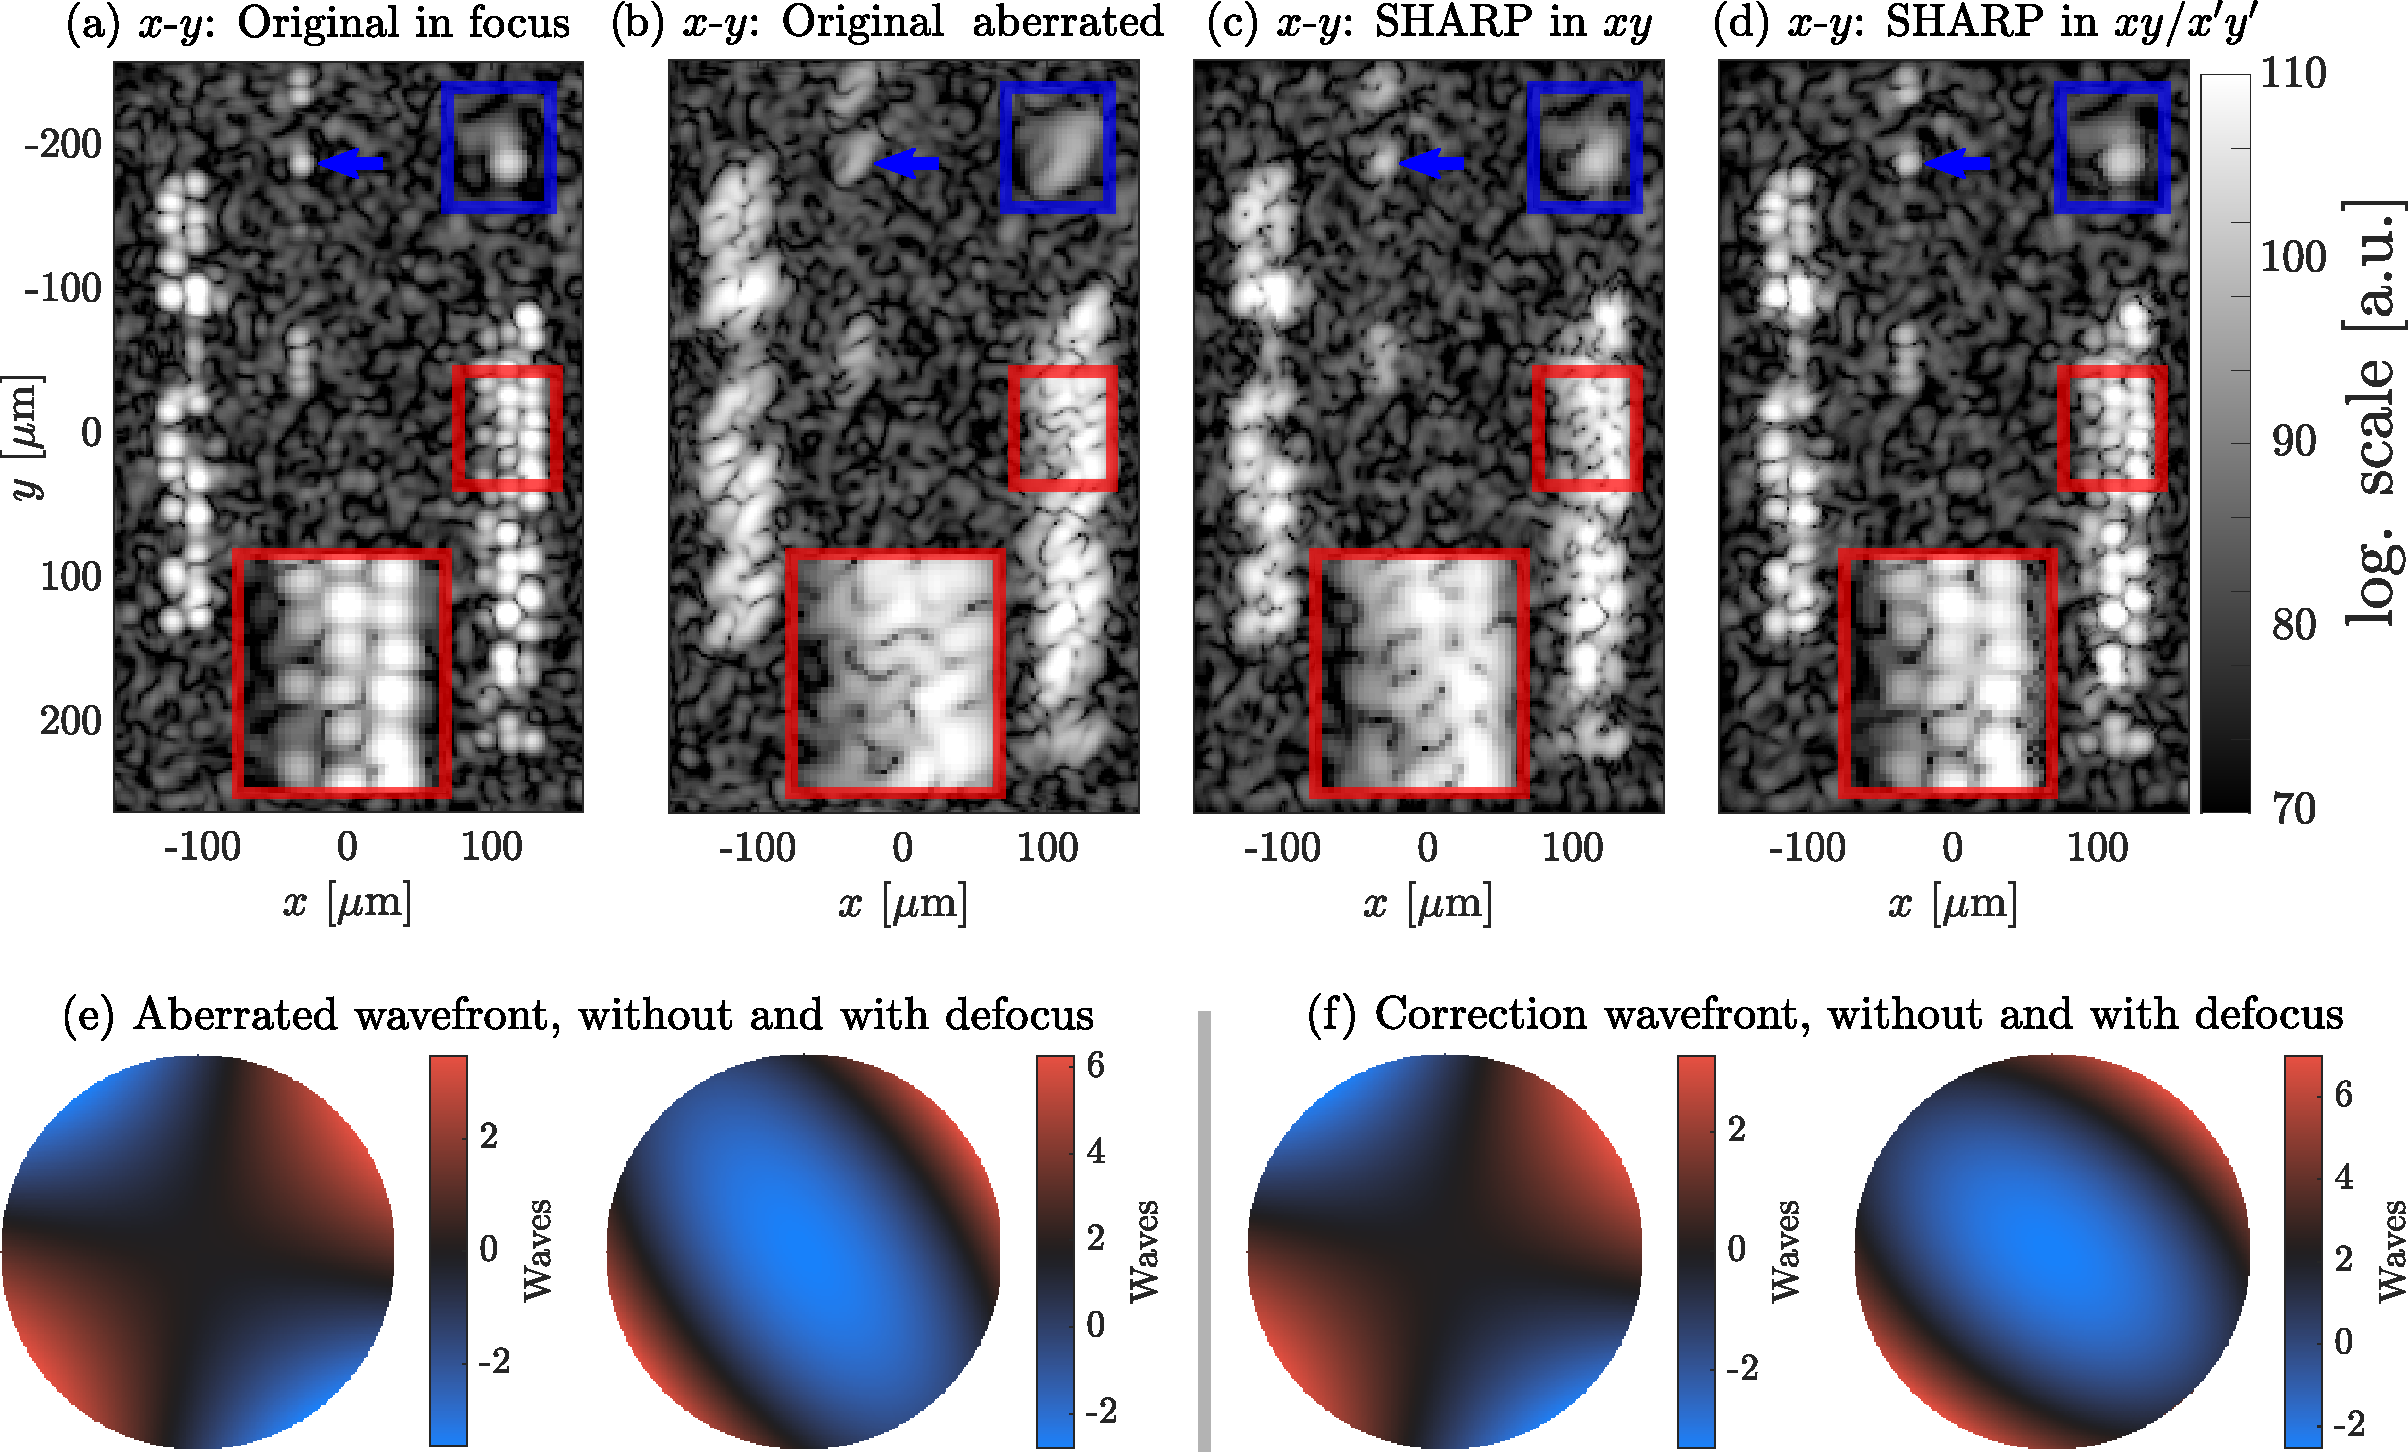
\includegraphics[width=\textwidth]{Figures/SHARP/SHARP45d_Int.pdf}
	\caption[Testing aberration correction with SHARP-$x'y'$ using a simulated OCT tomogram.]{Testing aberration correction with SHARP-$x'y'$ using a simulated OCT tomogram. \textit{En face} views of tomograms; (a) original in focus, (b) aberrated, (c) after SHARP-$xy$ and (d) subsequent SHARP-$x'y'$. Wavefront maps for the same \textit{en face} as before; (e) aberrated wavefront and (f) correction wavefront, without (left) and including defocus (right).}
	\label{fig:SHARP45d_Int}
\end{figure}

Phase noise comprising random offsets and slopes in the range $[0,\ 2\pi]$ was added to the aberrated tomogram. For describing the phase filter in 1D CAO, only Legendre polynomial $P_2$ was used. First, SHARP-$xy$ procedure was applied, obtaining partial aberration correction as visualized in the \textit{en face} plane of Fig.~\ref{fig:SHARP45d_Int}(c), followed by application of SHARP-$x'y'$ that resulted in a more noticeable image quality improvement due to aberration correction as noted in Fig.~\ref{fig:SHARP45d_Int}(d), and approaching the image quality of the original aberration-free tomogram, noted particularly when comparing the red and blue insets. Finally, the correction wavefront was computed as a superposition of the individual 1D corrections in the four axes [right panel in Fig.~\ref{fig:SHARP45d_Int}(f)] and its distribution shows that indeed correction of aberrations not oriented along the main axes $x$ and $y$ is feasible. Projection of the correction wavefront into Zernike basis yielded the weights $0.9\lambda$ for $Z_4$ and $2.2\lambda$ for $Z_5$, and using these weights to generate the correction wavefront without including defocus yields the wavefront in the left panel of Fig.~\ref{fig:SHARP45d_Int}(f).

To illustrate better the phase stabilization procedures performed along oblique axes, Figure~\ref{fig:SHARP45d_Phase} shows phase views of \textit{en face} and cross-sectional oblique planes of the original tomogram [Figs.~\ref{fig:SHARP45d_Phase}(a) and (d)], after correcting phase noise along $x'$ [Figs.~\ref{fig:SHARP45d_Phase}(b) and (e)] and along $y'$ [Figs.~\ref{fig:SHARP45d_Phase}(c) and (f)]. In the original phase images, 2D phase instability is clear. Instead, the \textit{en face} views after correcting phase noise exhibit 1D phase stability along the oblique axis. The oblique-planes images in Figs.~\ref{fig:SHARP45d_Phase}(d)-(f) showing the path marked by the white lines on the \textit{en faces}, also exhibit phase stability as expected. Interestingly, the analysis on the MPS [see Figs.~\ref{fig:SHARP45d_Phase}(g)-(i)] is yet valid for this case, only that the axis along which the MPS displays a Gaussian profile is now rotated, depending on the corrected axis.

\begin{figure}[htb!]
	\centering
	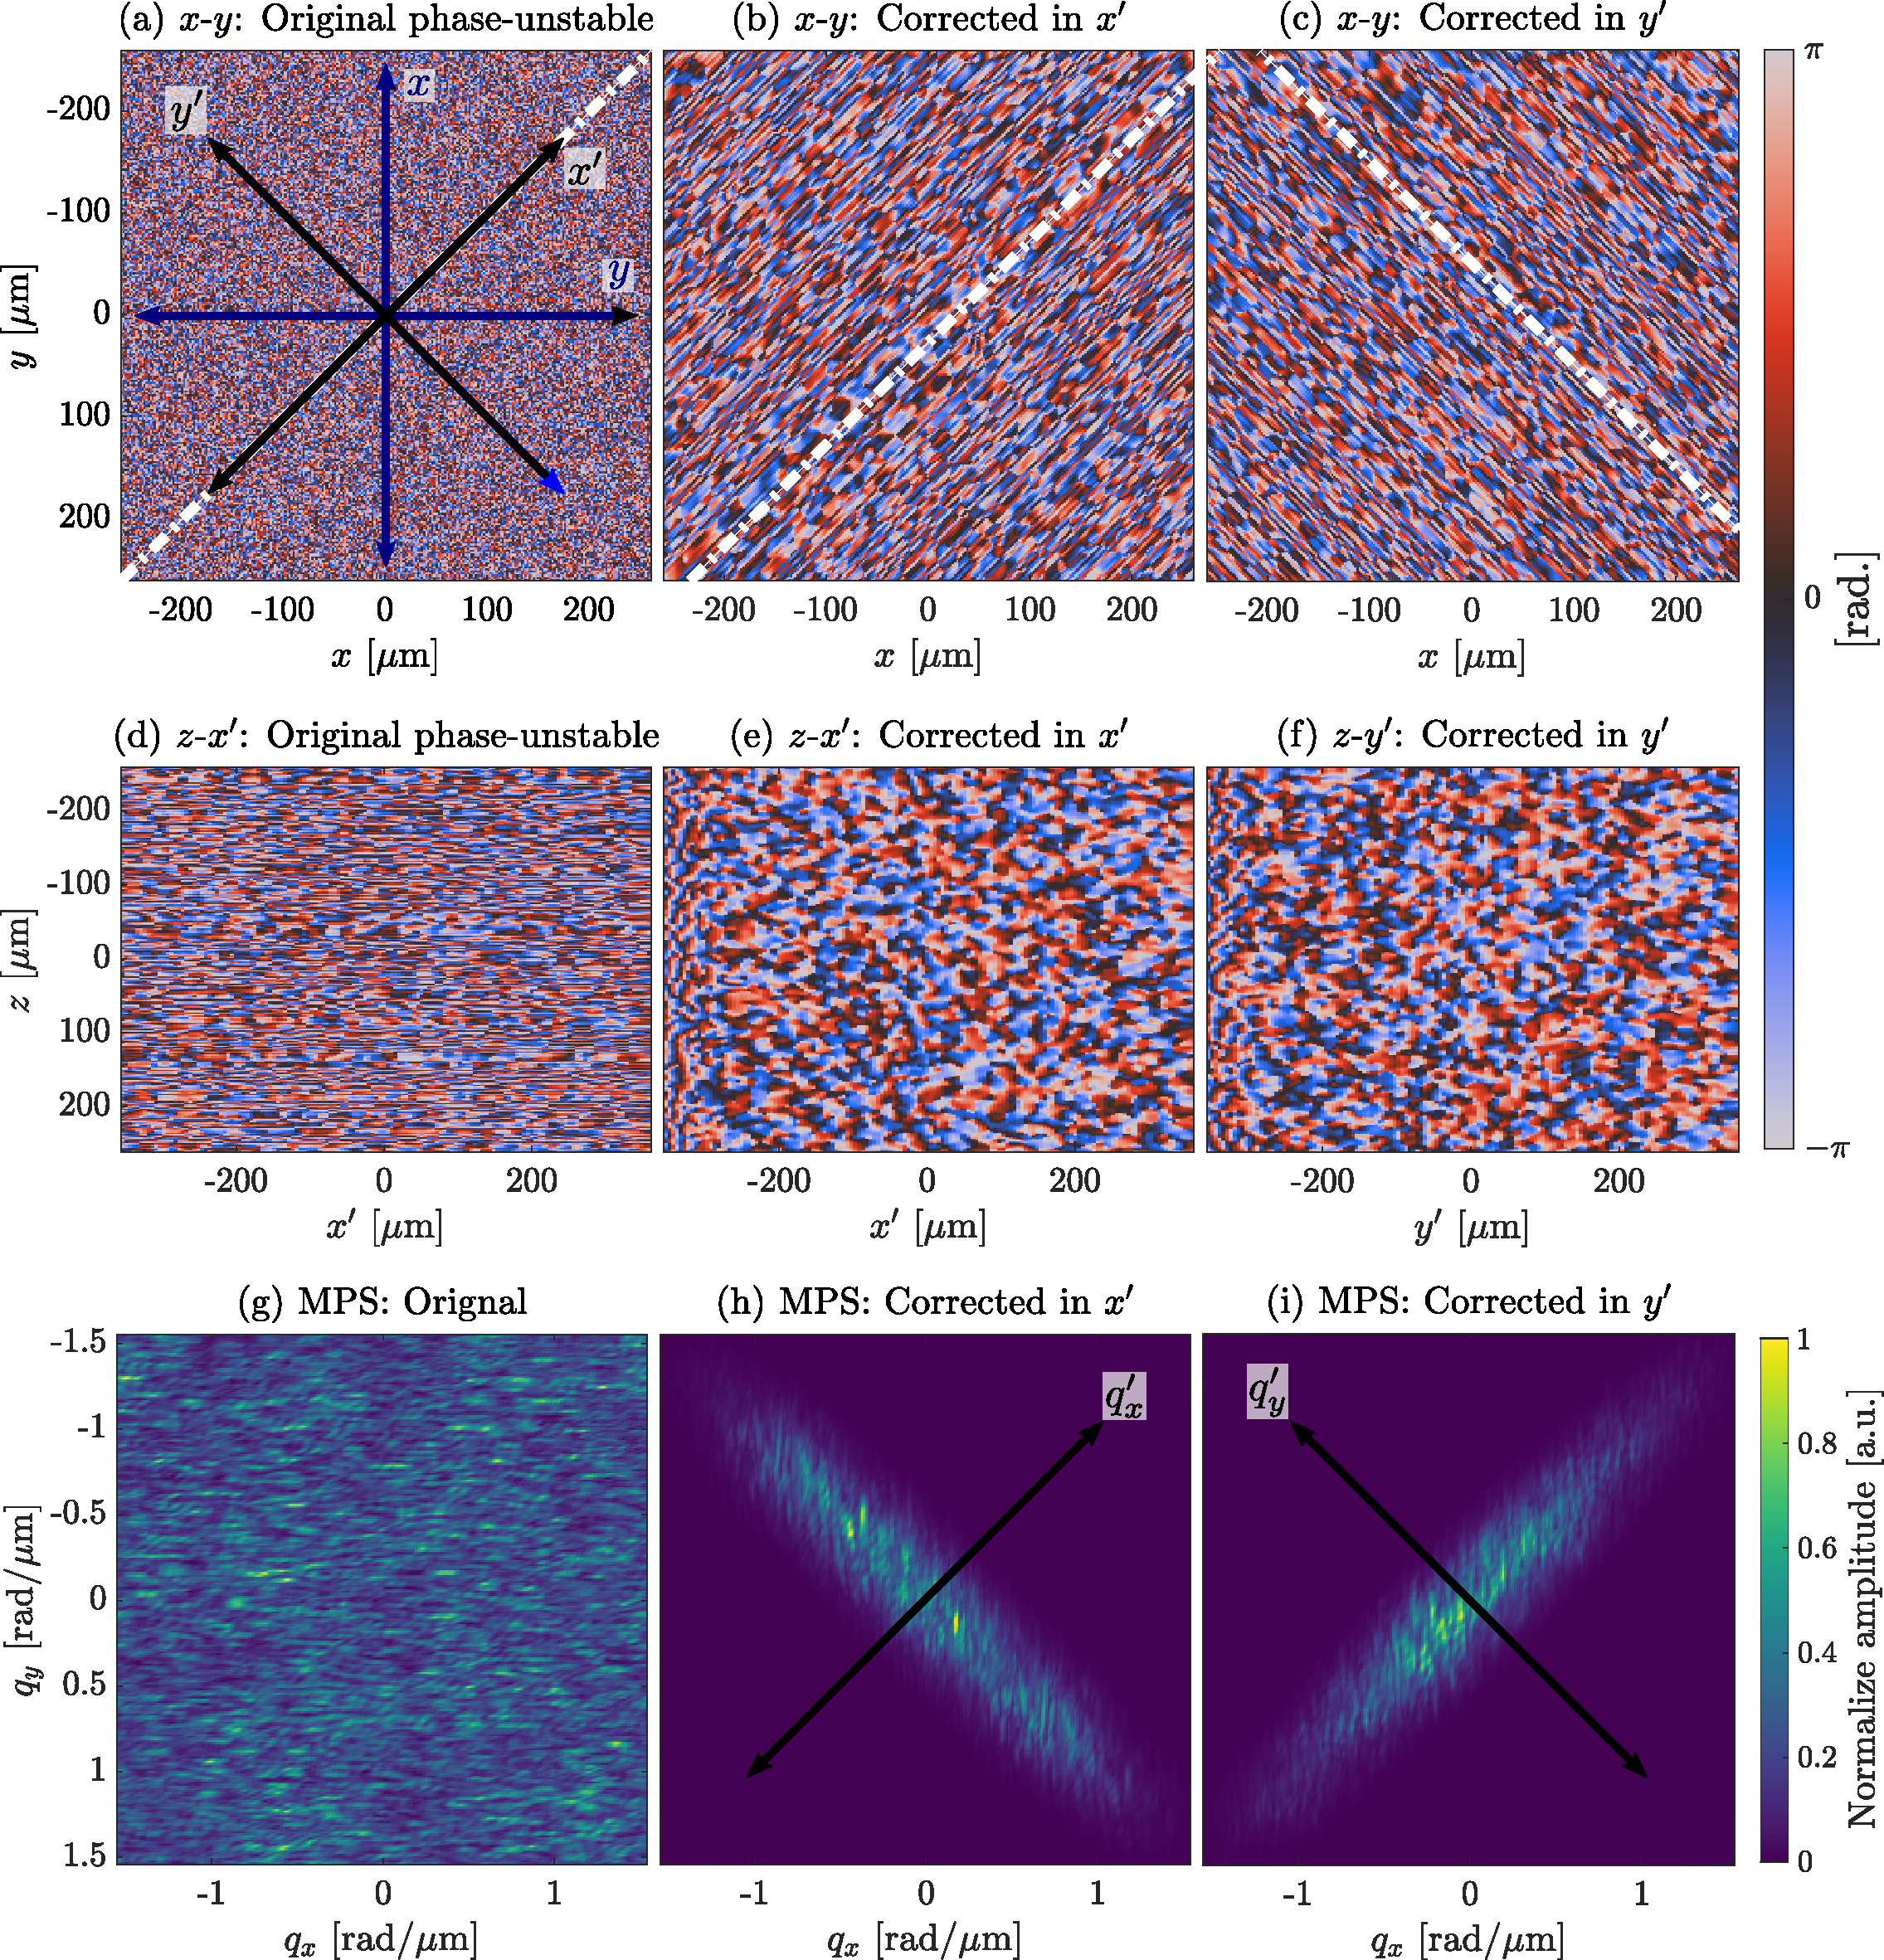
\includegraphics[width=\textwidth]{Figures/SHARP/SHARP45d_phase.pdf}
	\caption[Testing phase stabilization along oblique axes for a simulated OCT tomogram.]{Testing phase stabilization along oblique axes for a simulated OCT tomogram. \textit{En face} views of tomograms; (a) original, (b) corrected in $x'$ and (c) corrected in $y'$. Oblique cross-sections $z$-$x'$; (d) original and (e) corrected in $x'$. (f) Oblique cross-sections $z$-$y'$ corrected in $y'$. MPS of tomograms; (g) original, (h) corrected in $x'$ and (i) corrected in $y'$. Note that axes in the MPS maps are $q_x$, $q_y$ and not $q_{x'}$, $q_{y'}$.}
	\label{fig:SHARP45d_Phase}
\end{figure}

% When dofocus is the dominant aberration, independent results from SHARP-$xy$ and SHARP-$x'y'$ should be very similar given that the quadratic phase used to represent defocus can be fully described using either the main axes or the rotated ones. Therefore, a readily verification of SHARP-$x'y'$ in an experimental dataset could be performed using the OoF tomogram of the \textit{cucumis sativus} sample used in Section~\ref{sec:Test}, to complement the previous verification with the simulated dataset. Figure~\ref{fig:SHARP_EnfacesComp} shows an \textit{en face} plane of the original OoF tomogram in Fig.~\ref{fig:SHARP_EnfacesComp}(a), after SHARP-$xy$ in Fig.~\ref{fig:SHARP_EnfacesComp}(b) and after SHARP-$x'y'$ in Fig.~\ref{fig:SHARP_EnfacesComp}(d). Defocus of original image was successfully corrected with both procedures, showing its equivalence for defocus correction.

% Also, a experimental validion of  windows-based SHARP-$xy$ was also applied and show in Fig.~\ref{fig:SHARP_EnfacesComp}(c), obtaining that 

% \begin{figure}[htb!]
% 	\centering
% 	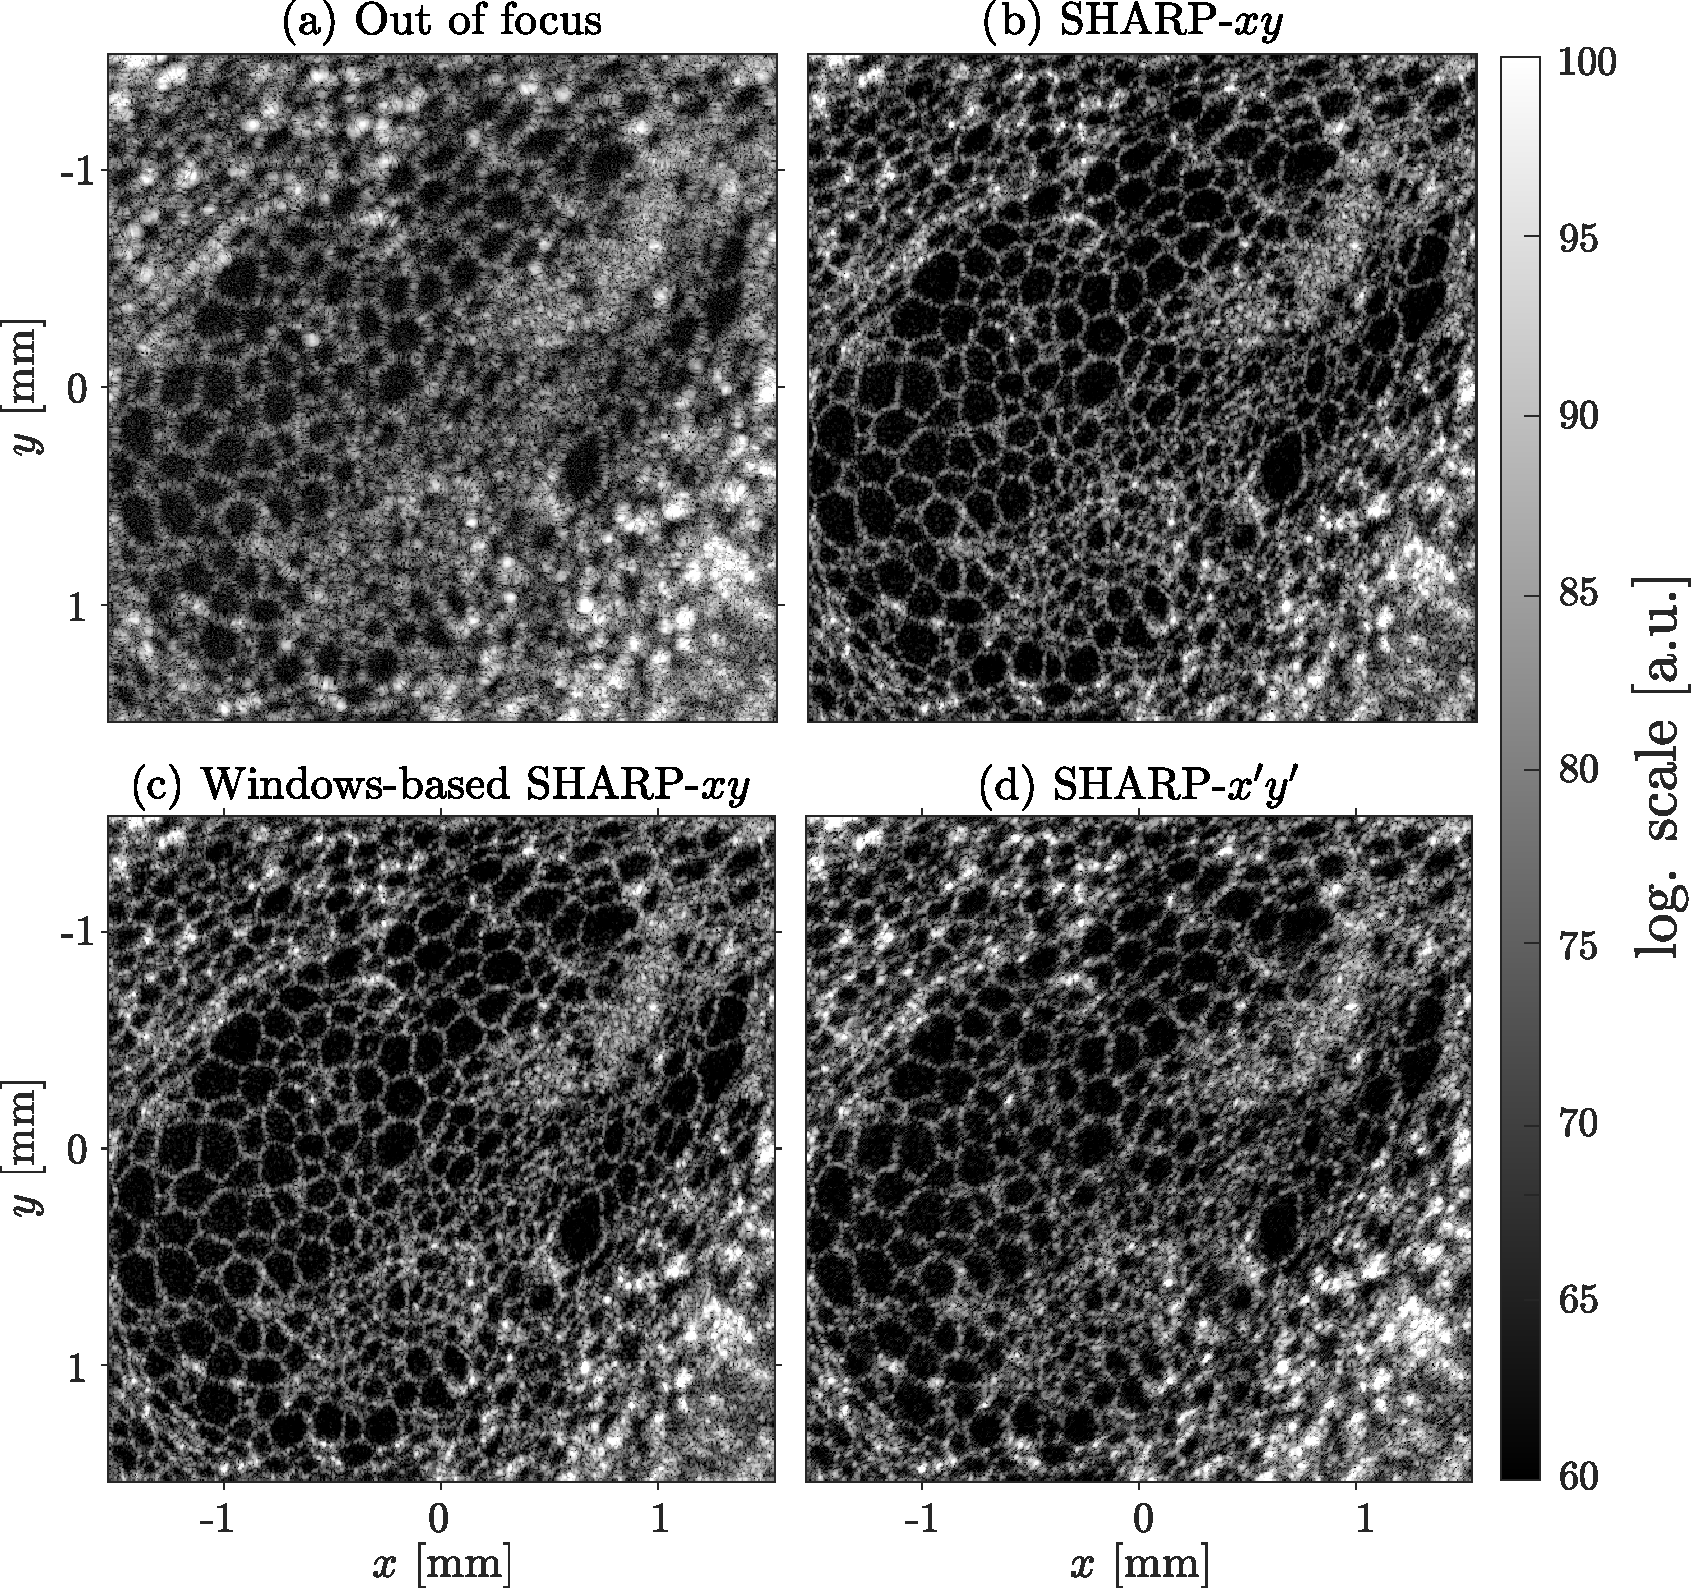
\includegraphics[width=.8\textwidth]{Figures/SHARP/SHARP_ExtensionsEnfaces.pdf}
% 	\caption[Testing phase stabilization along oblique axes for a simulated OCT tomogram.]{Testing phase stabilization along oblique axes for a simulated OCT tomogram. \text{En face} views of tomograms; (a) original in focus, (b) aberrated, (c) after SHARP-$xy$ and (d) SHARP-$x'y'$.}
% 	\label{fig:SHARP_EnfacesComp}
% \end{figure}

\FloatBarrier

\subsection{Computational aberration correction in polarization-sensitive OCT}

The operation of CAC techniques so far has been described for intensity images used for structural contrast, however, in functional extensions of OCT the effects of aberrations in the acquired complex signal is also transferred through the post-processing methods used for calculating additional useful information of the sample, such is the case of polarization-sensitive (PS-)OCT, which is used for the measurement of polarimetric properties of tissue~\cite{deBoer1997_Twodimensional, deBoer2017_Polarization}. PS-OCT has great clinical interest due to its sensitivity to fibrillar tissue and its organization, and is used in intravascular OCT~\cite{Villiger2018_Coronary}, retinal imaging~\cite{Elmaanaoui2011_Birefringence, Cense2009_Retinal}, anterior segment~\cite{Li2020_Vectorial}, among others applications. Adaptive optics (AO) has been integrated into PS-OCT systems for aberration-free retinal imaging with improved effective lateral resolution~\cite{Cense2009_Retinal}, however, it is known that AO does not extend the depth of field, whereas numerical alternative like ISAM or CAO are capable of extending the depth of field by correcting for the depth-dependent defocus. The phase stability requirement has hindered adoption of CAC technique in many systems oriented to PS-OCT that may not satisfy the phase stability requirement. Apart from the work of Davis \textit{et. al.} where they developed a vectorial description of ISAM for polarization-sensitive imaging~\cite{Davis2007_Nonparaxial, Davis2007_Polarimetric}, CAC techniques have not been demonstrated in PS-OCT, and thus it is unclear whether the processing performed in such techniques affects negatively the PS-OCT processing.

Given that SHARP can operate with phase-unstable systems, its operation can be extended to PS-OCT systems which often do not satisfy the phase stability requirement. In this section, a procedure to properly apply SHARP in PS-OCT taking into consideration the particularities of Stokes tomograms processing is presented. Because the theory and models used in PS-OCT are rather extensive and out of scope of this work, only the sufficient information required to understand the operation of SHARP in PS-OCT is provided here, and detailed information if required by the reader can be explored in addition bibliography~\cite{deBoer2017_Polarization, Villiger2013_Spectral}.

\subsubsection{Overview of Stokes processing}

In PS-OCT processing, briefly summarized in Figure~\ref{fig:PSOCTProc}, the polarimetric properties of the backscattered light by the sample are retrieved from a collection of several polarization-diverse measurements. More specifically, the sample is illuminated using two polarization states $p=\{p_1, p_2\}$ orthogonal in the Poincar\'e sphere and the backscattered signal is measured by a polarization-diverse receiver with two orthogonal polarization channels $c=\{c_1, c_2\}$, for a total of four tomographic complex measurements $S_{p,c}(x,y,z)$. In standard Stokes processing for PS-OCT, these four complex measurements forming two Jones vectors are converted into two Jones-Stokes vectors $\mathbf{\mathbb{S}} = [I, Q, U, V]^T$ composed of the four Stokes parameters from which polarimetric properties of the sample are calculated~\cite{deBoer2017_Polarization}, being $I$ the total intensity and $Q$, $U$ and $V$ quantities related to the degree of linear, oblique and circular polarization, when properly normalized. Polarimetric properties retrieved in Stokes processing are degree of polarization (DOP) and birefringence comprising phase retardation or retardance $\Delta n$ and optic-axis orientation $\psi$. 

%Polarization-diverse detection consist in placing a polarization-dependent beam splitter in the output of the interferometer to split the light into two orthogonal polarization states, typically horizontal and vertical states, and each one is detected by an independent detector. To generate the two illumination polarization states, advanced active elements are used like electro-optic modulator (OEM) to dynamically interchange the polarization state between pair of A-lines during the measurement, a method known as inter-A-line modulation, or passive elements like polarization delay units (PDU) that separates the light into two polarization states which are then delayed by a constant optical path length resulting in the two polarization states being depth-encoded in the acquired tomogram.

Because of the coherent nature of OCT signal, the Jones-Stokes vectors are affected by speckle which appears as strong noise in the subsequent calculation of polarimetric properties. For this reason, each Jones-Stokes parameter is spatially averaged, typically using a Gaussian kernel, to produce incoherent Stokes parameters $\mathbf{\bar{\mathbb{S}}}~=~[\bar{I}, \bar{Q}, \bar{U}, \bar{V}]^T$ with reduced speckle resulting in polarimetric properties with reduced noise. However, a resolution loss is associated to this spatial average, which in combination to aberrations have imposed a relatively coarse lateral resolution in PS-OCT imaging~\cite{Cense2009_Retinal}, making difficult to obtain highly-localized measurement of polarimetric properties of tissue which may be of great interest~\cite{Cense2009_Retinal, Li2020_Vectorial}.

\begin{figure}[htb!]
	\centering
	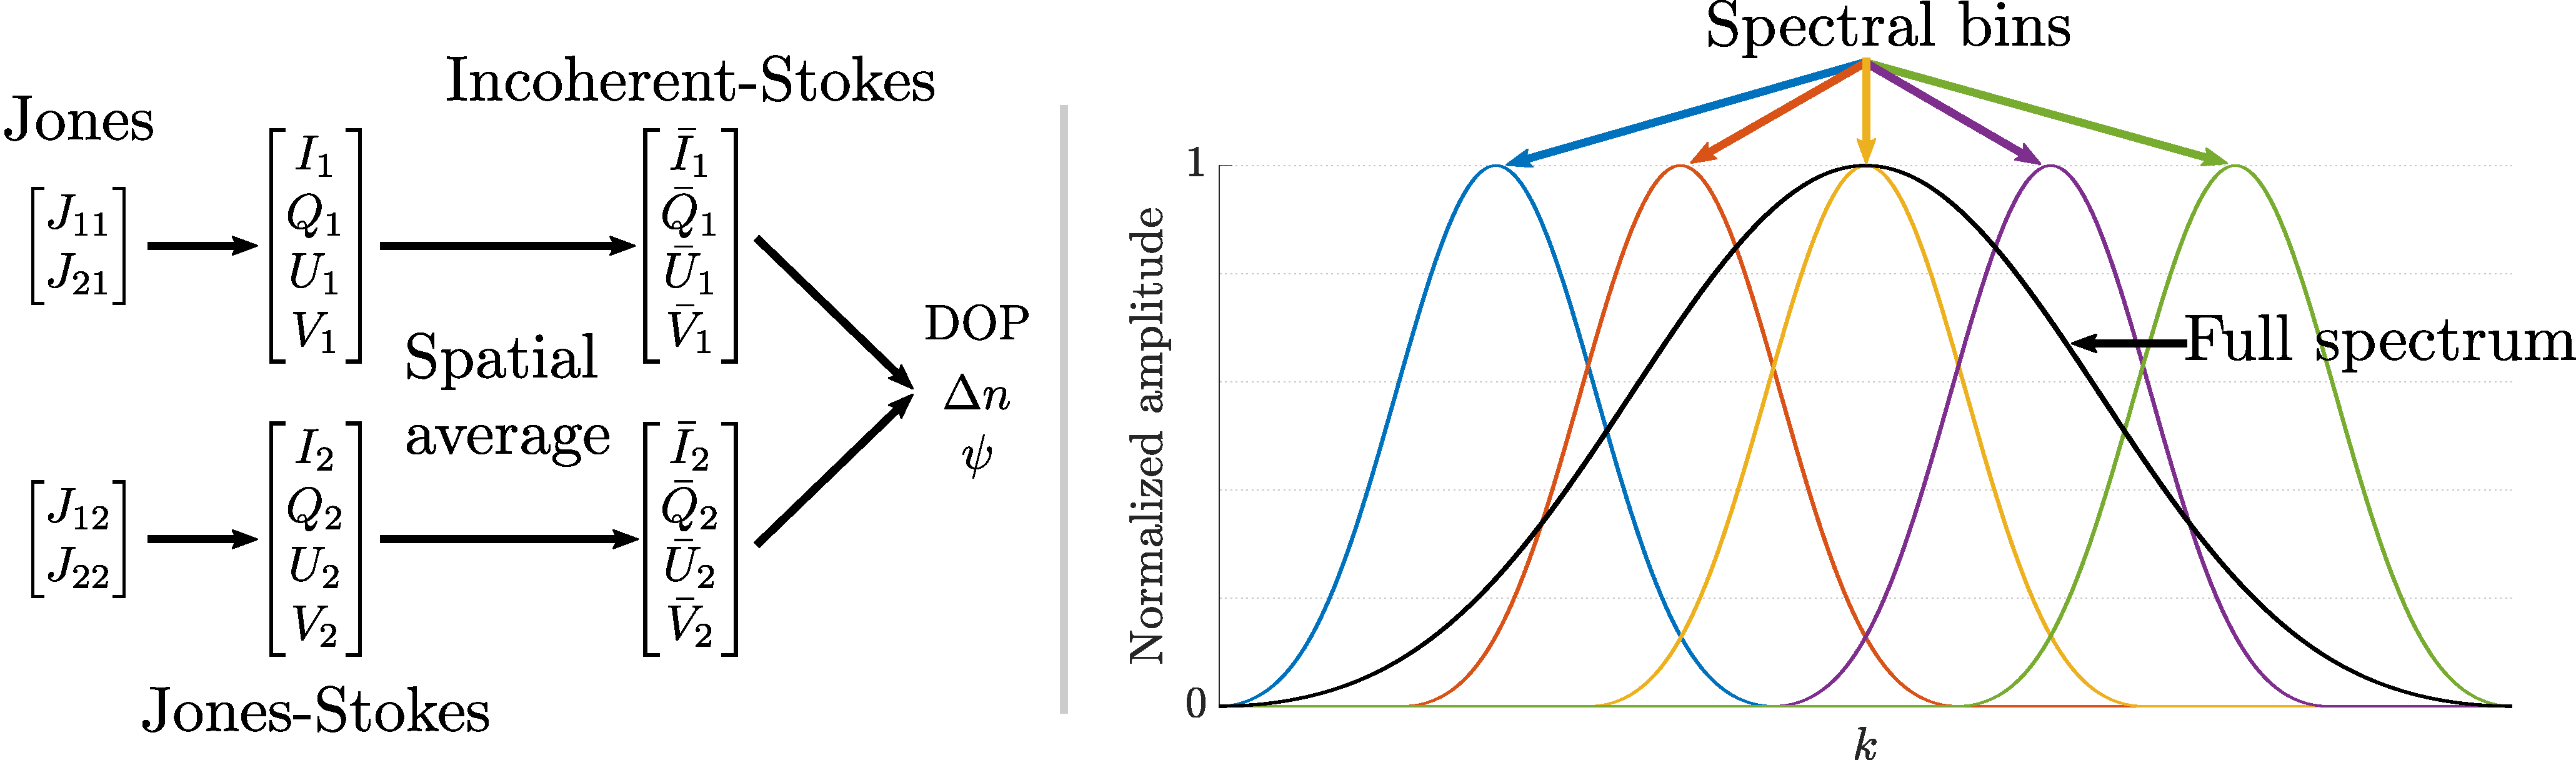
\includegraphics[width=\textwidth]{Figures/SHARP/PSOCT-Processing.pdf}
	\caption[Overwiew of Stokes processing for PS-OCT and spectral binning.]{Overwiew of Stokes proccesing for PS-OCT and spectral binning.}
	\label{fig:PSOCTProc}
\end{figure}

In certain PS-OCT systems, fiber-based components induce wavelength-dependent changes on the polarization state of light that prevent to obtain reliable information from the acquired signals $S_{p,c}(x,y,z)$ directly~\cite{deBoer2017_Polarization}. To overcome this, spectral binning processing has been proposed~\cite{Villiger2013_Spectral}, in which the acquired spectral signals $S_{p,c}(x,y;k)$ in $k$-space are splitted into several bins covering smaller portions of the bandwidth, as depicted in Fig.~\ref{fig:PSOCTProc}, such that wavelength-dependent effect of the system is made more constant within each spectral bin since they have a narrower bandwidth than the original spectrum. Then, PS-OCT processing is performed independently for each reduced-bandwidth tomogram, with additional steps based on vectorial analysis to align the estimated polarimetric properties into a single estimation comprising the information of the entire original spectrum~\cite{Villiger2013_Spectral}. There is an additional resolution loss in spectral binning processing, but this time in the axial direction only, because the bandwidth of each spectral bin is narrower than the original spectrum, resulting in a coarser axial resolution.

\subsubsection{Polarization-sensitive SHARP}

Given that aberration correction operates on the complex field, SHARP must be applied on the four complex tomograms $S_{p,c}$ prior to conversion to Stokes parameters which are intensity values. Particularities of the process are following explained, but first, it should be clarified that the goal here is to correct non-polarizing aberrations, which are different to polarization aberrations that include changes in the polarization state of light associated with ray paths through optical systems~\cite{Chipman1989_Polarization}.

The determination of the optimal weights for CAO from individual spectral bins tends to be ineffective since each spectral bin has a reduced axial resolution and different amount of signal-to-noise ratio. Therefore, the tomogram with the full spectral bandwidth of the system is employed to determine the optimal weights via optimization rather than finding the optimal weights for each spectral bin independently. The optimization procedure is performed only for a single polarization state $p$ and the image sharpness metric is calculated from the total intensity given by $|S_{p,c1}|^2 + |S_{p,c2}|^2$, assuming that aberrations are polarization-independent thus they are the same for both polarization states. Strictly speaking, polarizing media may induce undesired changes in wavefront that depend on the polarization state of light, but magnitude of these changes have generally a small contribution compared to wavefront aberrations, even more with the magnitude of polarizing effects of tissue.

Phase offsets and slopes required for phase stabilization are determined also in the full-bandwidth tomogram but for the two polarization states $p$ independently because phase noise is not necessarily the same. After determining phase noise correction (offsets and slopes) and the optimal weights for aberration correction using the full-bandwidth tomograms, these parameters are then applied to all spectral bins and input polarization states. To summarize, operation of SHARP in PS-OCT consists in determining the parameters for phase noise and aberration correction in the full-bandwidth tomograms and then using those to correct each spectral bin independently. This is possible since the filter applied in CAO is $k$-independent and since phase noise correction operates on each A-line globally and therefore it does not change across spectral bins. Aberration-corrected complex tomograms  $\tilde{S}_{p,c}$ for each spectral bin are then transformed into Stokes vectors followed by the subsequent steps in PS-OCT processing. The positive effect of CAO applied to the complex tomograms is translated into the Stokes parameters and ultimately into the polarimetric properties.

\section{Complex noise reduction: CTNode}\label{sec:CTNode}

High sensitivity of typically $\sim$100~dB is provided by OCT system, meaning that backscattered light as weak as $10^{-10}$ times the reference mirror reflection can still be detected~\cite{Choma2003_Sensitivity, deBoer2003_Improved}. Further improvements are possible with post-processing, and most used approach consists in averaging multiple frames to reduce noise, taking advantage of the high imaging speed provided by FDOCT that enables to acquire multiple repeated frames~\cite{Baumann2019_Signal, Szkulmowski2013_Averaging}. Averaging can be either incoherent, i.e. using the intensity signal, or coherent, i.e. using the complex signal, but it has been found that coherent averaging is more efficient in improving the SNR in phase stable data~\cite{Baumann2019_Signal}. Although frame averaging has been effective to increase SNR of OCT images for an improved visualization and diagnosis~\cite{Sakamoto2008_SpectralDomain}, it demands the acquisition of multiple frames which is unpractical in certain scenarios, specially in volumetric imaging given the large amount of data, the significant increase in acquisition time and the susceptibility to be negatively affected by motion artifacts. 

Analyzing and addressing noise in complex signal is advantageous for phase-dependent post-processing techniques~\cite{Uribe-Patarroyo2020_Noise}. In particular, in CAC there is an explicit interest in improving SNR because aberrations produce a significant reduction of signal collection, and as a consequence acquired images have a reduced dynamic range that is not expanded by aberration correction. The optimum amplitude filter integrated in SHARP is a straightforward tool to address noise and although its performance could be improved by means of oversampling, its effectiveness is limited specially when sampling approaches Nyquist.

In this section, a statistical approach for noise reduction is proposed as an alternative to current strategies, in which the 2D or volumetric information of the tomogram is exploited to reduce noise with no need of frames repetitions. The framework of this proposal is based on the previously developed technique \textbf{T}omographic \textbf{NO}n-local means \textbf{de}speckling (TNode) that suppresses speckle on the intensity while preserving resolution~\cite{Cuartas-Velez2018_Volumetric}, except that here the aim is to denoise the complex signal thus the new proposal is called \textbf{C}oherent \textbf{T}omographic \textbf{NO}n-local means \textbf{de}noising (CTNode). A description of CTNode is provided below.

\subsection{Non-local means}

Non-local means has been used widely in image processing in several fields~\cite{Deledalle2015_NLSAR,Lu2012_Nonlocal,Yu2016_Probabilitybased,Coupe2008_Optimized} as it outperforms traditional averaging in resolution preservation. The core idea behind non-local means is to perform a spatial average using an adaptive kernel defined explicit for each pixel of the image using the information of neighboring pixels~\cite{Cuartas-Velez2018_Volumetric}. To define the weights of the kernel used to filter a target pixel, a statistical metric is used to determine how similar are each neighboring pixel to the target pixel. Defining the acquired noisy tomogram as $S_N(\bm{r})$ with $\bm{r}$ being a 3D vector representing the three coordinates $\bm{r}=(x,y,z)$, the weighted estimation $\hat{S}(\bm{r})$ of the noiseles signal $S(\bm{r})$ is computed as
\begin{equation}\label{eq:NLM}
    \hat{S}(\mathbf{r}) = \frac{\sum_{\bm{r}'\in \bm{\nu}} w(\bm{r}, \bm{r}') S_N(\bm{r}')}{\sum_{\bm{r}'\in \bm{\nu}} w(\bm{r}, \bm{r}')}
\end{equation}
where $w(\bm{r}, \bm{r}')$ are the weights of target pixel $\bm{r}$ with respect to all neighbor pixels $\bm{r}'$ inside a search windows $\bm{\nu}$. The search windows $\bm{\nu}$ is a collection of pixels centered at $\bm{r}$ with sizes $(\nu_x, \nu_y, \nu_z)$ for a total size of $V=(2\nu_x+1)\times(2\nu_y+1)\times(2\nu_z+1)$ that defines the spatial extension of the filtering kernel. In order words, the search window controls how many pixels are included in the weighted average of target pixel. The following step is to find a proper definition of $w(\bm{r}, \bm{r}')$ based on statistical properties of noise in order to produce an appropriate filtering.

\subsection{Derivation of weights for noise reduction}

Noise in FDOCT is originated in the acquisition of the spectral fringes under an additive model, allowing to express the measured noisy signal in $k$-space as $s_n(x,y,k) = s(x,y,k) + n(x,y,k)$ where $s(x,y,k)$ is the true noiseless signal and $n(x,y,z)$ is the randomly distributed noise. After Fourier transform of the spectral fringes used to compute the depth-dependent signal $S_N(x,y,k)$, noise still follows an additive model since
\begin{align}
    \text{FT}_k\{s_n(x,y,k)\} &= \text{FT}_k\{s(x,y,k)\} + \text{FT}_k\{n(x,y,k)\} \nonumber\\
    S_N(\mathbf{r}) &= S(\mathbf{r}) + N(\mathbf{r}),
\end{align}
where $S(\mathbf{r})$ is the true noiseless depth-dependent signal and $N(\mathbf{r})$ the additive noise, setting $\mathbf{r} = (x,y,z)$ for simplicity as before. The task is therefore to cancel out the contribution of noise. It has been shown that noise in OCT follows a zero-mean complex Gaussian distribution with equal standard deviation $\sigma_N$ on both the real and imaginary parts~\cite{Makita2016_Noiseimmune, Uribe-Patarroyo2020_Noise}. Analyzing only the real part of the signal $R_N = \text{Re}\{S_N\}$ by now, the probability of measuring a realization $R_N$ given a true value $R = \text{Re}\{S\}$ and the standard deviation $\sigma_N$ of noise is~\cite{Deledalle2012_How}
\begin{equation}\label{eq:GaussianProb}
    \mathcal{P}(R_N|R, \sigma_N) = \frac{1}{\sqrt{2\pi}\sigma_N} \exp\left\{-\frac{(R_N-R) ^ 2} {2\sigma_N^2}\right\}
\end{equation}
and similarly for the imaginary part $I_N = \text{Im}\{S_N\}$.

To determine the similarity between a pair of values $R_N(\bm{r})$ and $R_N(\bm{r}')$, a similarity criterion is defined using the likelihood-ratio test (LRT),
\begin{equation}
    \mathcal{L}\{R_N(\bm{r}), R(\bm{r})\} = \frac{\mathcal{P}[R_N(\bm{r})|R(\bm{r},\bm{r}'), \sigma_N] \mathcal{P}[R_N(\bm{r}')|R(\bm{r},\bm{r}'), \sigma_N]} {\mathcal{P}[R_N(\bm{r})|R(\bm{r}), \sigma_N] \mathcal{P}[R_N(\bm{r}')|R(\bm{r}'), \sigma_N]}
\end{equation}
which evaluates the probability that the underlying noiseless parameters $R(\bm{r})$ and $R(\bm{r}')$ are different between them or equal to a common parameter $R(\bm{r}, \bm{r}')$. The standard deviation of noise is assumed equal in all probabilities given that $\sigma_N$ tends to be constant over the entire tomogram. More specifically, the numerator of the LRT is the probability of the two values $R_N(\bm{r})$ and $R_N(\bm{r}')$ being different realizations of the same distribution, in which case the similarly is high and the numerator tends to one, while the denominator is the probability of the two values $R_N(\bm{r})$ and $R_N(\bm{r}')$ being realizations of different distributions, in which case the similarity is small and the denominator tends to a large value. In consequence, the LRT tends to one when the two pixels being compared are likely similar and to zero when they are dissimilar.

In practice, the underlying parameters are in general unknown and the LRT cannot be computed directly, therefore it is replaced by the generalized likelihood ratio (GLR) $\mathcal{L}_G$~\cite{Cuartas-Velez2018_Volumetric} where the parameters are changed by their maximum likelihood estimates~\cite{Deledalle2012_How}, enabling to obtain a closed-form expression given by
\begin{equation}\label{eq:GLR}
    \mathcal{L}_G\left\{R_N(\bm{r}), R_N(\bm{r}')\right\} = \exp\left\{-\frac{[R_N(\bm{r}) - R_N(\bm{r}')]^2} {4\sigma_N^2}\right\}
\end{equation}
for the case of the Gaussian distribution of Eq.~\eqref{eq:GaussianProb}. The GLR in Eq,\eqref{eq:GLR} was derived using the real part of the signal, but the expression for the imaginary part is equivalent. The probability of the real and imaginary parts must be compounded in order to avoid corruptions in the phase due to dissimilar filtering. This compounding imposes the condition that two pixels are similar only when the real \textit{and} imaginary parts are similar. Hence, the GLR for the complex signal $\mathcal{L}_C$ is
\begin{align}\label{eq:GLR_total}
    \mathcal{L}_C\left\{S_N(\bm{r}), S_N(\bm{r}')\right\} &= \exp\left\{-\frac{[R_N(\bm{r}) - R_N(\bm{r}')]^2} {4\sigma_N^2}\right\} \exp\left\{-\frac{[I_N(\bm{r}) - I_N(\bm{r}')]^2} {4\sigma_N^2}\right\} \nonumber\\
    &=  \exp\left\{-\frac{[R_N(\bm{r}) - R_N(\bm{r}')]^2 + [I_N(\bm{r}) - I_N(\bm{r}')]^2} {4\sigma_N^2}\right\} \nonumber\\
    &= \exp\left\{-\frac{|S_N(\bm{r}) - S_N(\bm{r}')|^2} {4\sigma_N^2}\right\},
\end{align}
where the property of complex numbers $|\mathcal{Z}|^2 = \text{Re}\left\{\mathcal{Z}\right\}^2 + \text{Im}\left\{\mathcal{Z}\right\}^2$ was employed. $\mathcal{L}_C$ depends only in the two observed values $S_N(\bm{r})$, $S_N(\bm{r}')$ and the standard variation of noise that can be estimated experimentally. 

The GLR is a point-wise estimation but comparing patches of pixels around the two pixels of interest could yield a more robust estimation. Similarity between patches $\mathcal{L}_{P}$ is calculated by computing the point-wise similarity between corresponding pixels of the patches and then compounding the logarithmic probabilities as
\begin{equation}
    \mathcal{L}_{P}\left\{S_N(\bm{r}), S(\bm{r}')\right\} = \sum_{\bm{\tau}\in\bm{p}}\log\{\mathcal{L}_C[S_N(\bm{r}+\bm{\tau}), S_N(\bm{r}'+\bm{\tau})]\}
\end{equation}
where $\bm{p}$ is a collection of 3D shifts such that $\bm{r}+\bm{\tau}$ and $\bm{r}'+\bm{\tau}$ span the pixels in the patches around $\bm{r}$ and $\bm{r'}$, respectively, which are called similarity windows having sizes $(p_x, p_y, p_z)$ and total size $P=(2p_x+1)\times(2p_y+1)\times(2p_z+1)$.

Finally, the expression for the weights in Eq.~\eqref{eq:NLM} is 
\begin{equation}
    w(\bm{r}, \bm{r}') = \exp\left[\frac{\mathcal{L}_{P}\left\{S_N(\bm{r}), S_N(\bm{r}')\right\}}{h}\right]
\end{equation}
where an additional parameter $h>0$ is introduce to modify the distribution of weights and control the overall filtering. Additionally, because the weight of the self-similarity $w(\bm{r}, \bm{r}')$ is significantly larger than any other weight, it is replaced by the maximum similarity found in the patch to obtain a better performance~\cite{Cuartas-Velez2018_Volumetric}.

To summarize, to estimate the noiseless value of each pixel, CTNode performs a non-local means around a search window centered in the target pixel, using weights calculated based on the similarity between pixels inside a similarity window, as is depicted for two patches in Figure~\ref{fig:CTNodeScheme} in a 2D arrangement, although 3D similarity and search windows can be used, depending on the information available. 

\begin{figure}[htb!]
	\centering
	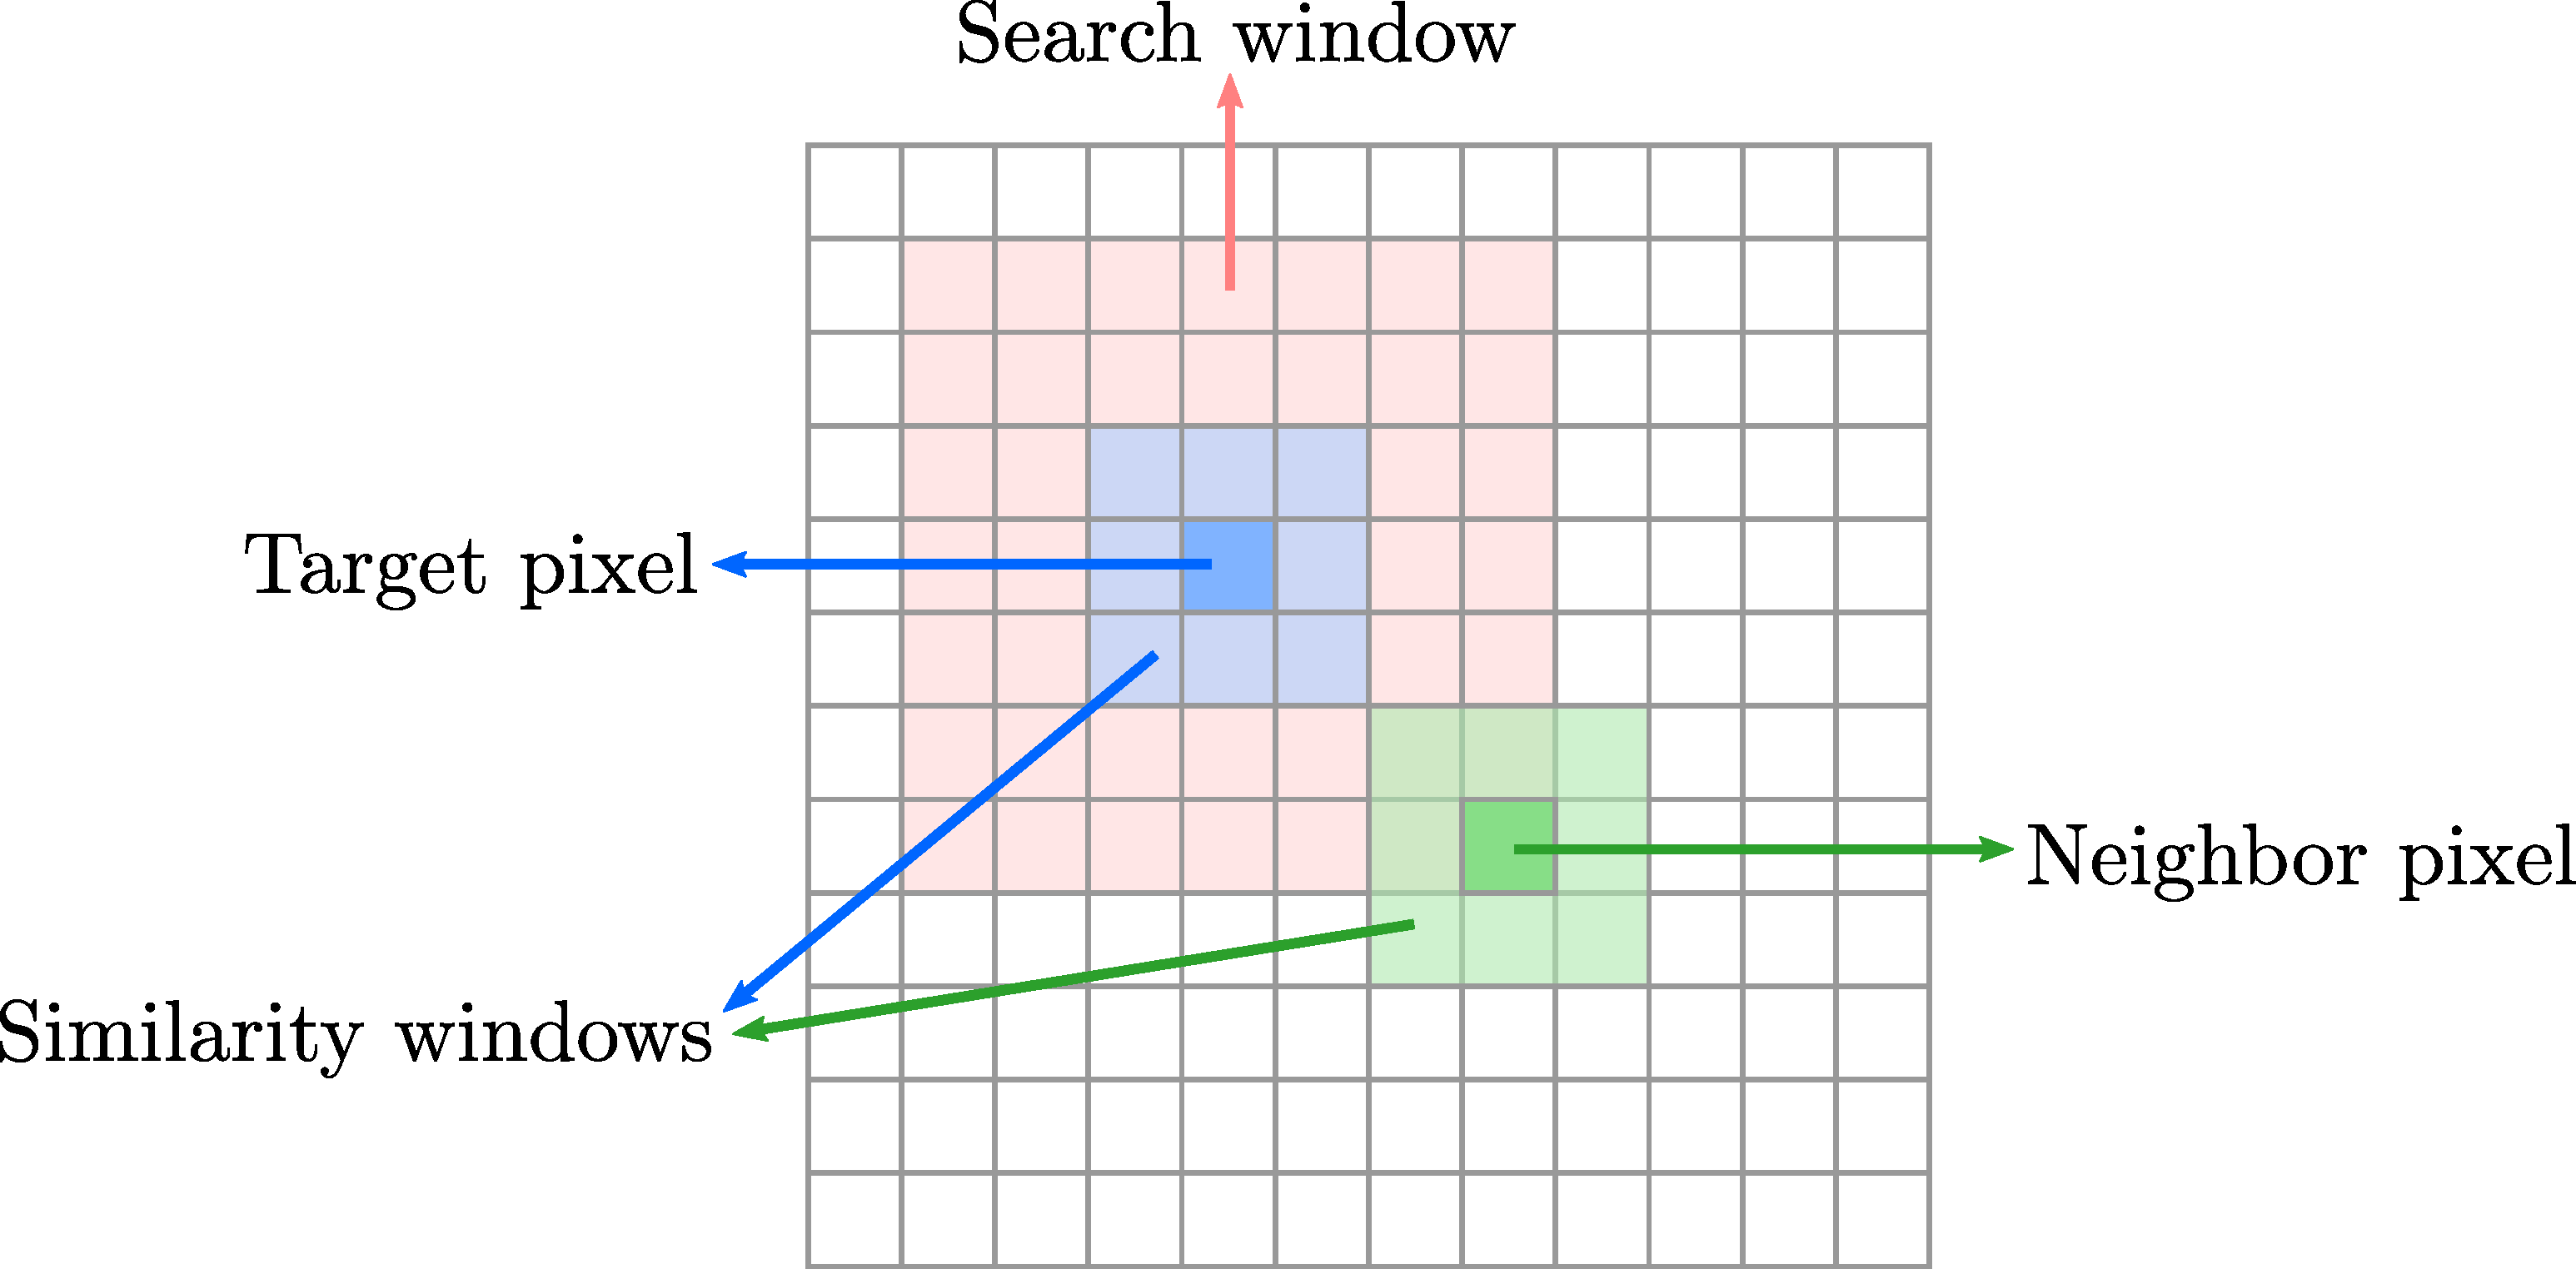
\includegraphics[width=.8\textwidth]{Figures/SHARP/CTNodeScheme.pdf}
	\caption[Illustration of the operation of non-local means.]{Illustration of the operation of non-local means using search window of size 7$\times$7 and similarity windows of size 3$\times$3.}
	\label{fig:CTNodeScheme}
\end{figure}

The purpose of CTNode in the context of this work is to complement SHARP to increase dynamic range of aberration-corrected images. Actually, reduction of complex noise could benefit subsequent operation of SHARP improving the procedure of optimizing image quality in CAO steps in regions with low SNR. Furthermore, there is a wide variety of applications yet to explore where CTNode could also be beneficial, in particular in phase-dependent or complex signal-based techniques like angiography~\cite{Makita2016_Noiseimmune}, flowmetry~\cite{Uribe-Patarroyo2014_Quantitative} and elastography~\cite{Wang2007_Phasesensitive} in which sensitivity is greatly influenced by noise level thus pre-processing the complex signal with CTNode could boots subsequent performance of these techniques, with no need of acquiring multiple repetitions frames as demanded in traditional averaging.

\subsection{Evaluation of CTNode in simulated OCT signal}

To evaluate CTNode, it is desirable to have a noise-free reference but it is in principle impossible to achieve experimentally, therefore, the noise-free simulated OCT tomogram used previously was employed for this purpose. Figure~\ref{fig:CTNode_Sim_int} shows a selected B-scan from the original tomogram in Fig.~\ref{fig:CTNode_Sim_int}(a), showing the cross-section of the bright-intensity cylindrical objects, immersed in the low-intensity nearly homogeneous medium that constitute the tomogram. Synthetic zero-mean Gaussian noise was added to the real and imaginary parts of the noiseless simulated tomogram with a constant variance $\sigma_N^2$ over the entire tomogram, as illustrated with the noisy B-scan of Fig.~\ref{fig:CTNode_Sim_int}(b). There is a signal decay over depth in the original tomogram emulating light absorption, although it may not be obvious in Fig.~\ref{fig:CTNode_Sim_int}(a). This signal decay causes a variation of SNR despite $\sigma_N$ being constant, as can be appreciated in the logarithmic SNR map shown in Fig.~\ref{fig:CTNode_Sim_int}(c), where a threshold was used to display only values greater than $-3$~dB, corresponding to 0.5 in linear scale, which means that the signal level is half the noise variance, hence signal is masked by noise. A limit for the SNR of the minimum detectable signal is 0~dB (1 in linear scale) meaning that the signal level is equal to noise variance.

\begin{figure}[htb!]
	\centering
	\includegraphics[width=\textwidth]{Figures/SHARP/CTNode_Sim_int.pdf}
	\caption[Evaluating performance of CTNode in a simulated OCT tomogram.]{Evaluating performance of CTNode in a simulated OCT tomogram. Intensity B-scan planes: (a) Original noise-free (b) noisy with zero-mean Gaussian noise, (d) after CTNode, after (e) coherent and (f) incoherent averaging. (c) Logarithmic SNR for B-scan in (b) threshold to show only values $>-3$~dB.}
	\label{fig:CTNode_Sim_int}
\end{figure}

Then, CTNode was applied to the noisy tomogram. It was found that the use of large search and similarity windows yields strong noise reduction but at the cost of degrading resolution because the filtering kernel is large and prone to smear information. Conversely, resolution is better preserved using small windows but filtering efficiency is reduced. Furthermore, a large value of $h$ is desired for an efficient noise reduction but it causes a strong filtering of high SNR pixels which are expected to be slightly filtered since effect of noise is not significant. These observations are expected from the general operation of non-local means algorithm and in particular from the operation of TNode for speckle suppression~\cite{Cuartas-Velez2018_Volumetric}. Parameters were iteratively tuned by visual inspection of results seeking for an optimal trade-off between the thee competing aspects: efficient noise reduction, resolution preservation and avoidance of corruption of pixels with high SNR, resulting in a search window of 15$\times$15$\times$15, a similarity window of 3$\times$3$\times$3 and a filtering parameter $h=0.10$. Processing time was about 8~seconds per B-scan of size 160$\times$256~px$^2$, in a workstation computer running on an Intel core i7-8700 processor @~3.2GHz, using a GPU-based implementation in MATLAB 2019a running on a 6~GB GPU NVIDIA P4000.

For comparison, images using coherent and incoherent frames averaging were also computed. The set of repetition frames was created by replicating the noiseless B-scan, then adding synthetic noise to each repetition with the same variance and finally computing the arithmetic mean of the complex signal for coherent averaging and of the intensity signal for incoherence averaging. It is known that coherent averaging of $N$ frames produces a reduction of noise variance by a factor of $1/N$ whereas incoherent averaging only of $1/\sqrt{N}$, however, coherent averaging also reduces signal level resulting in a less SNR improvement than expected, although it is still higher than improvement achieved by incoherent averaging~\cite{Baumann2019_Signal}. For this test, $N$ was set to 12, a value at which coherent averaging performed similar to CTNode. 

Fig.~\ref{fig:CTNode_Sim_int}(d)-(e) shows the noisy B-scan after CTNode, coherent and incoherent averaging, respectively. There is not any signal degradation after CTNode suggesting that its application to the tomogram did not produce any detrimental effect in signal quality, and indeed there is a clear overall reduction of noise level as supposed, compared to noisy B-scan. For the following analysis, two regimes can be identified, one where SNR is below 0~dB and other where SNR is above 0~dB. For $\text{SNR}>0$, CTNode and coherent averaging recovered the underlying signal at an acceptable level, allowing to visually distinguish the speckle pattern from the noise, and in particular the upper dark band can be distinguished from the object information. For incoherent averaging, the speckle pattern is also visually perceptible but the contrast is greatly reduced because in this approach the noise floor level is not reduced, only the noise variance, contrary to coherent average approach where both the noise mean and variance are reduced~\cite{Baumann2019_Signal}. In all cases, the bight intensity structures appear unchanged, as is expected given that noise reduction is less significant when SNR is high. For this reason, noise reduction in intended to improve contrast in regions with SNR approaching to zero, whereas in regions with high SNR it is unlikely necessary because contribution of noise is unimportant. 

For $\text{SNR}<0$~dB, it can be observed that despite the noise reduction, underlying signal information is lost in all filtering approaches, since in this regime the mean intensity signal is below the noise variance and therefore underlying true signal cannot be distinguishable from noise. In fact, it is possible to increase negative SNRs values using coherent average and for this case it was achieved at $N=100$ which is a relatively large and possibly unpractical amount.

The relevance of complex noise reduction is not only evident in intensity images in terms of contrast improvement but also in phase information that is very susceptible to noise. Figure~\ref{fig:CTNode_Sim_Phase} shows phase images of the B-scan plane used for Fig.~\ref{fig:CTNode_Sim_int}, of the original and noisy tomogram in Figs.~\ref{fig:CTNode_Sim_Phase}(a) and (b). Speckle pattern is directly visualized in noiseless phase B-scan, whereas noisy phase shows regions dominated by noise, and even in the high SNR regions noise is perceptible, making difficult the visualization of speckle pattern. Phase B-scans after CTNode and coherent averaging are shown in Fig.~\ref{fig:CTNode_Sim_Phase}(c) and (d), respectively, and both exhibit a reduction of noise in high and low SNR regimes, recovering the speckle pattern lost in low SNR regions and improving visualization of high SNR regions. 

% \begin{figure}[htb!]
% 	\centering
% 	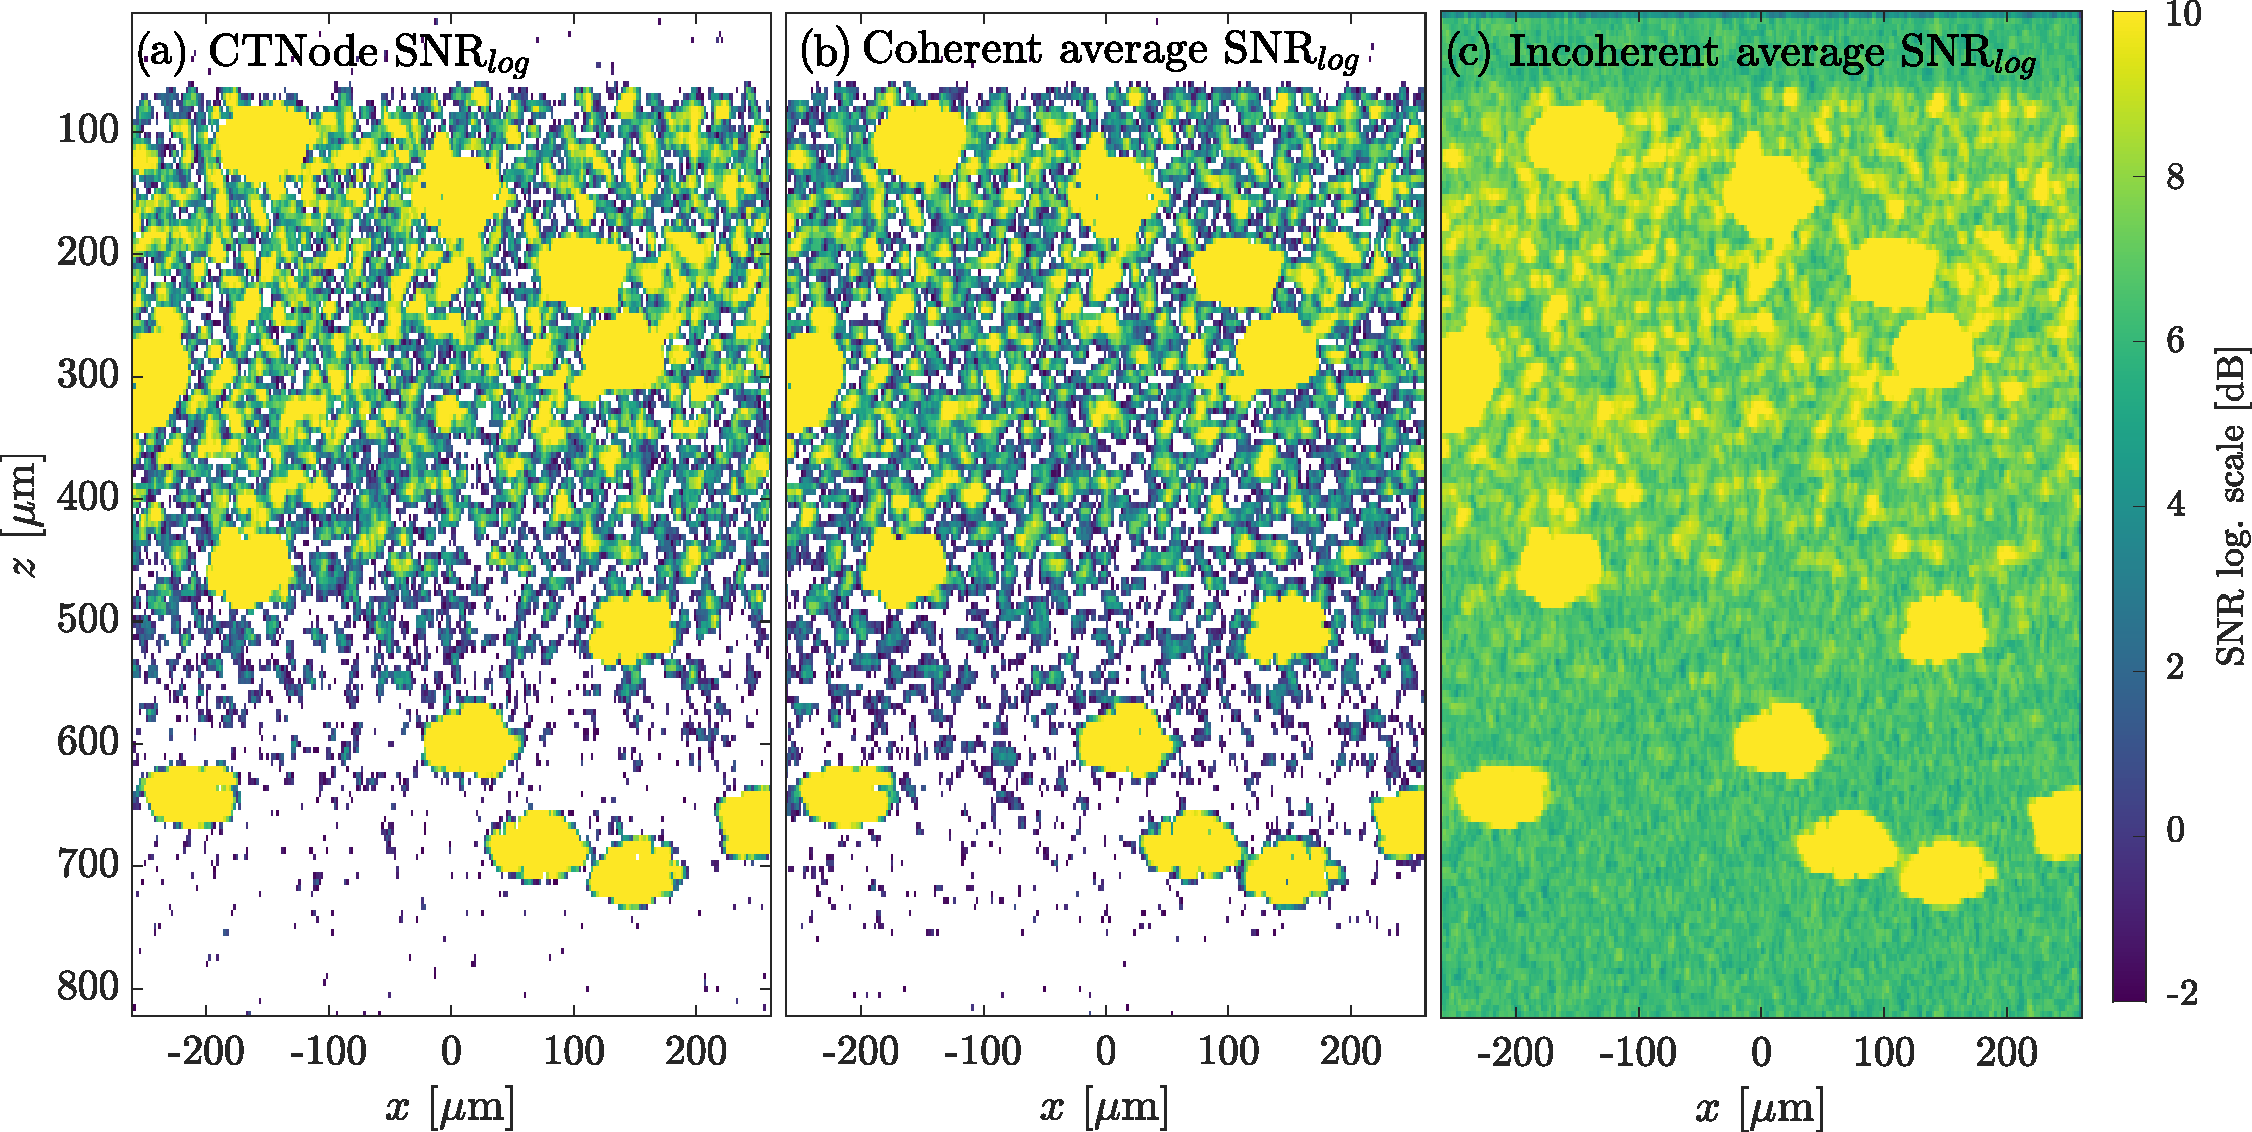
\includegraphics[width=\textwidth]{Figures/SHARP/CTNode_Sim_SNR.pdf}
% 	\caption[.]{.}
% 	\label{fig:CTNode_Sim_SNR}
% \end{figure}

\begin{figure}[htb!]
	\centering
	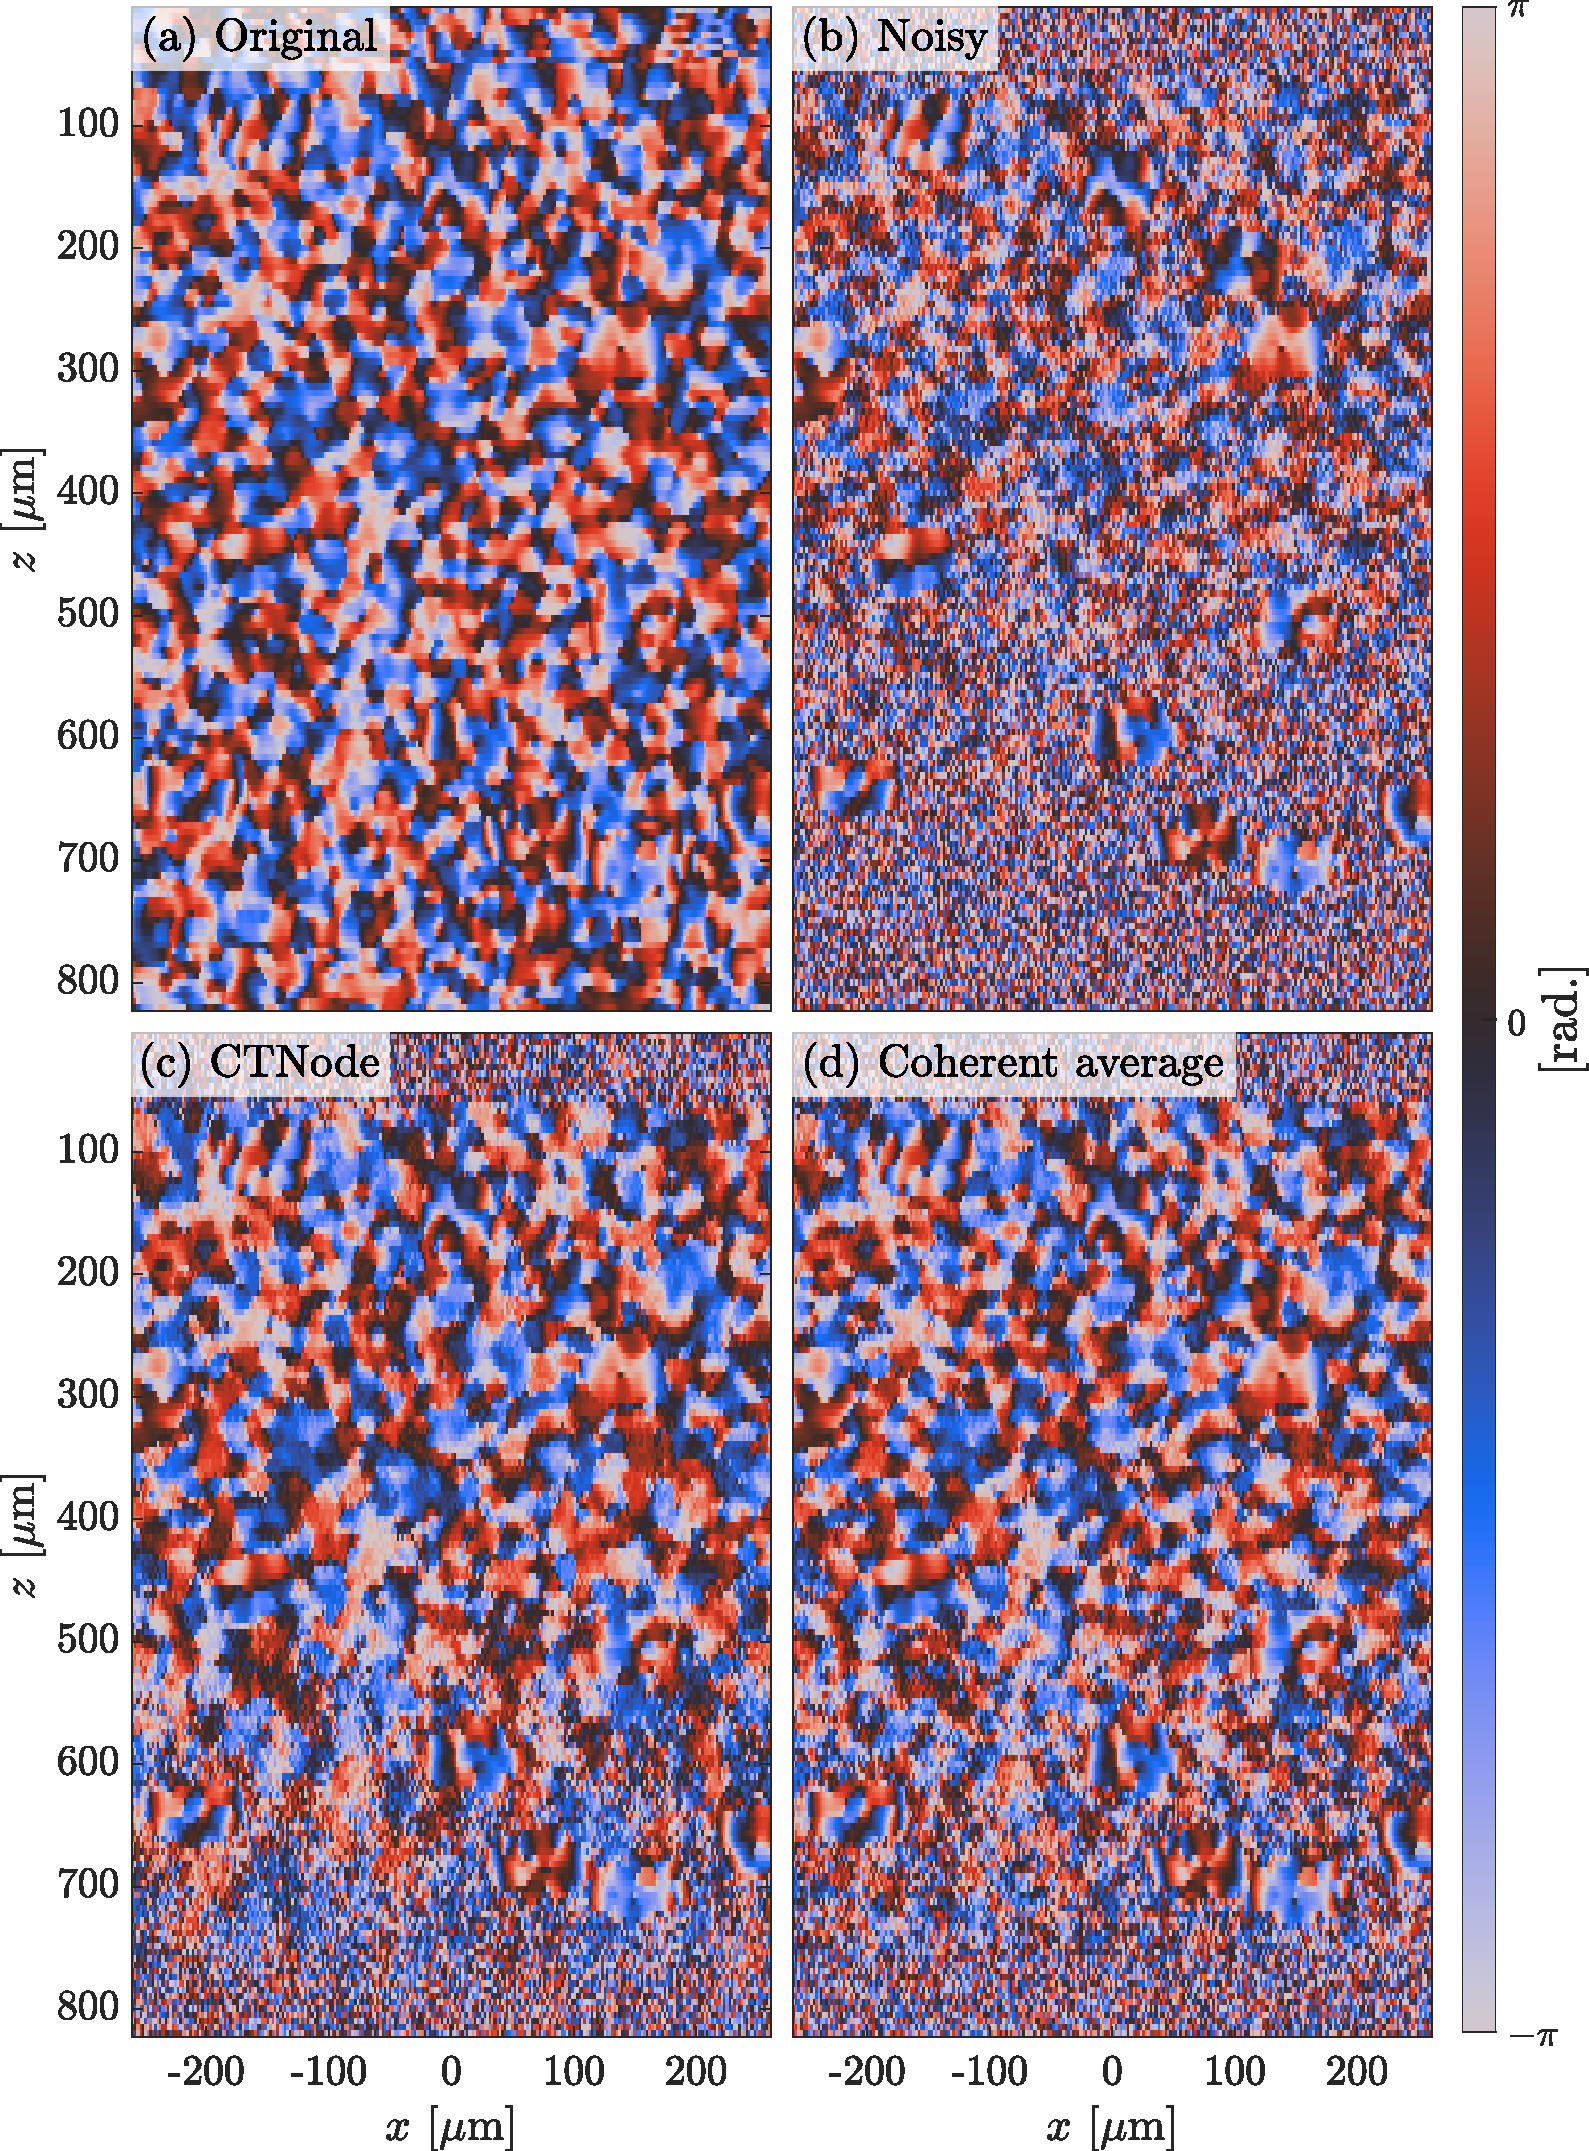
\includegraphics[width=.7\textwidth]{Figures/SHARP/CTNode_Sim_Phase.pdf}
	\caption[Evaluating reduction of Gaussian noise in phase information with CTNode in a simulated OCT tomogram.]{Evaluating reduction of Gaussian noise in phase information with CTNode in a simulated OCT tomogram. B-scan phase images: (a) Original noise-free, (b) noisy with zero-mean Gaussian noise and then filtered (c) with CTNode and (d) with coherent wavering.}
	\label{fig:CTNode_Sim_Phase}
\end{figure}

Although with current implementation of CTNode it appears to be unfeasible to filter pixels with negative SNRs to recover the underlying signal properly, it is clear that CTNode outperforms coherent averaging in the sense that it required a single repetition to obtain a similar result of averaging $12$ repetitions, given that CTNode (and non-local means in general) efficiently exploits the available information. It is expectable that extension of CTNode to operate with multiple frame repetitions, like it is possible with TNode currently, could boost its operation even more compared to arithmetic frame averaging. Anyhow, the possibility to efficiently reduce complex noise with a single acquisition is attractive for phase-dependent techniques where multiple repetition of frames is not practical given its specific acquisition scenarios~\cite{Uribe-Patarroyo2020_Noise}.

%\newpage
\phantomsection
%\chapter{Computational adaptive optics for phase unstable OCT systems}
\chapter{Complex shot noise reduction in OCT: CTN\lowercase{ode}}\label{chap:CTNode}

\iffalse
\section{SHARP: A CAO technique for OCT}

\subsection{Phase stability assessment}

\subsection{Description of the method}

\section{Proof of concept experimental validation}

\section{Extending SHARP}

\subsection{Motion artifacts correction}

\subsection{Spatially-varying aberrations correction}

\subsection{Complex amplitude noise reduction}
\fi
\newpage
\phantomsection
\chapter{Experimental applications}\label{chap:results}

In the previous chapter, the SHARP technique was explained in detail, including additional steps and modifications to address specific issues encountered in certain instances, as well as a proof of concept experimental validation using a straightforward to image sample with prominent structures, convenient to readily visualize and verify computational refocusing. Also, the CTNode technique was described and evaluated with a simulated tomogram.  In this chapter, experimental operation of SHARP is demonstrated with samples with medical relevance including \textit{ex vivo} and \textit{in vivo} imaging, to show the potential of SHARP to improve the quality of OCT tomograms in order to provide more detailed information of tissue and to facilitate visualization of images for an improved analysis of specialists, more importantly in intensity-based imaging but in polarization-sensitive imaging as well. Additionally, experimental application of SHARP is complemented with the previously developed technique TNode and the new proposal CTNode, to provide a more significant improvement of image visualization.

First experimental demonstration is presented in anterior segment imaging of an excised swine eye, where SHARP is complemented with TNode and CTNode independently, being this an application with great relevance in OCT given that the anterior segment possesses structures with fundamental roles for vision, including cornea, limbus, iris, sclera, among others. An additional demonstration of performance of CTNode is then presented in human retina \textit{in vivo}, independently of SHARP.  A second demonstration of SHARP is presented in catheter-based imaging, which is the second largest imaging modality in OCT after ophthalmic-OCT, using a dataset from the airway of a swine acquired \textit{in vivo}. An additional \textit{in vivo} demonstration is showed in skin imaging of human hand dorsal where involuntary sample motion arising from pulse heartbeat and respiration must be corrected. Finally, the operation of SHARP in polarization-sensitive OCT is demonstrated in the limbal region of the excised swine eye, showing computational refocusing of polarimetric parameters.

The experimental data-sets of the anterior segment and human skin were acquired with the bench-top system used for the proof of concept experiment, varying in some cases the scan lens and sampling configuration accordingly. The endoscopic dataset was provided by NinePoint Medical. The human retina dataset was acquired with a bench-top retinal SSOCT system integrated in a modified commercial ophthalmic interface~\cite{Braaf2018_Complex}. Specific relevant parameters used in each experiment are described in the corresponding section.

\section{Anterior segment imaging \textit{ex vivo}}

The eyeball is in general divided into two main sections for its study; the anterior segment depicted in Figure~\ref{fig:eyeSchematic} and the posterior segment. The former is primary responsible for light collection and image formation by the cornea and the lens, and there are additional functional structures that support the normal operation of the eye including the iris, sclera, and ciliary body. OCT systems  for anterior segment imaging typically have a large depth of field of $\sim$3~mm to provide focused images across the entire axial extent of the anterior segment that is relatively large, but this implies a coarse lateral resolution. In some cases, the local structure of specific tissue is desired, for instance in the study of corneal layers thickness and stroma arrangement~\cite{Huang2015_Anterior}, achievable using high-resolution systems at the cost of having a relatively short depth of field.

\begin{figure}[htb!]
	\centering
	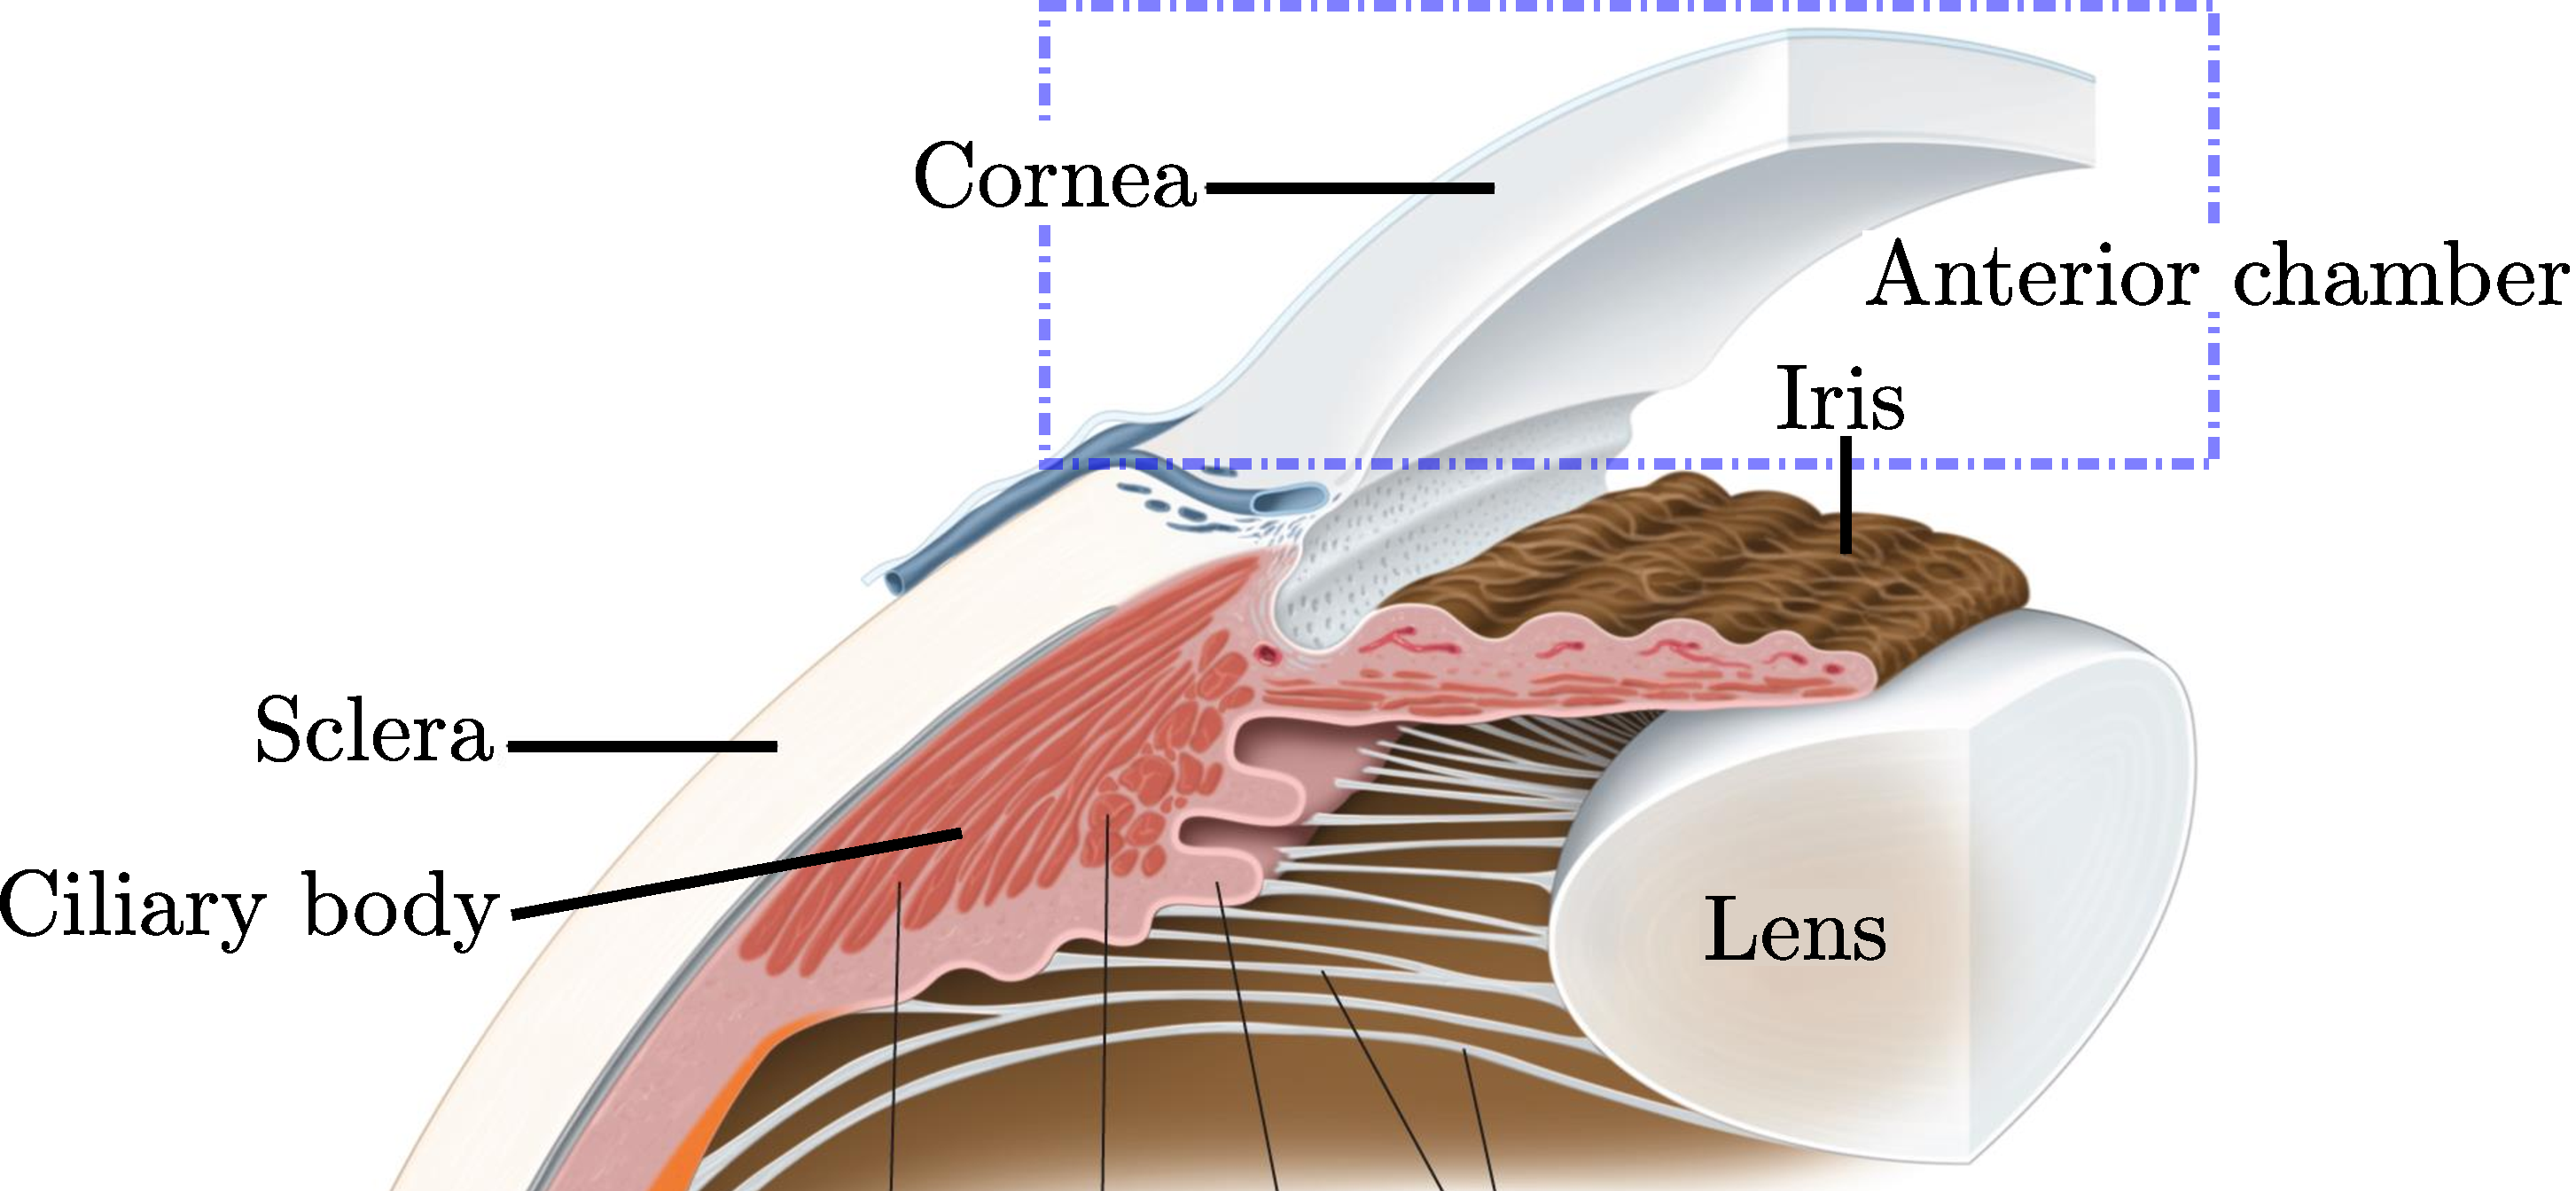
\includegraphics[width=.65\textwidth]{Figures/Results/EyeSchematic.pdf}
	\caption[Illustration of anterior segment anatomy.]{Illustration of anterior segment anatomy. [Adapted from \href{https://www.aao.org/image/anterior-segment-anatomy}{$\copyright$ 2020 American Academy of Ophthalmology}].}
	\label{fig:eyeSchematic}
\end{figure}

Computational refocusing has potential to extend the depth of field in anterior segment imaging in order to provide images with high lateral resolution in an extended depth covering a larger axial range of anterior segment~\cite{Wang2019_Cellular}. As an initial experimental demonstration, the SSOCT system used in the proof of concept experiment previously described was used to image the anterior segment of an excised swine eye, emphasizing in the cornea, around a region similar to that enclosed by blue rectangle in Fig.~\ref{fig:eyeSchematic}. From the measured tomogram, an ROI of 700 samples per A-line, 768 A-lines per B-scan and 256 B-scans was selected, covering a lateral field of view of 6$\times$2~mm$^2$ in an axial ranging of 4~mm in air. Two data-sets were acquired; a reference tomogram with the focal plane located at the paracentral zone of the cornea, and an OoF tomogram with the focal plane located at the iris, not visualized in the selected ROI. Figure~\ref{fig:ASImaging}(a) shows a B-scan of the original tomogram where defocus is evident in all the corneal layers and structures inside the stroma. Due to the confocal gating, there is a drop in signal-to-noise ratio (SNR) due to the large offset from the focal plane, observed as a low contrast between signal level in corneal tissue and noise floor level in regions having not signal from tissue.

Standard SHARP procedure was applied to the OoF tomogram, using Legendre polynomials $P_2,\ P_3,\ P_4,$ and $P_5$. The correction weights in $y$ were set equal to those found in $x$ given that the optimization procedure in $y$ was prone to fail at certain planes, possibly because there is not enough signal information for a robust estimation of the image quality metric, since the FoV in $y$ is small and the structures are oriented toward the $y$ axis. Fig.~\ref{fig:ASImaging}(b) shows that using the optimum filter [$\tilde{\Omega}(q_x,q_y)$] alone (i.e. setting phase filter $\tilde{\varphi}$ to zero) is very effective at reducing noise in this particular case where SNR in intrinsically low, achieving a floor noise reduction of $\sim$6~dB, which improves overall contrast. However, optimum filter alone does not improve the blur, contrary to Fig.~\ref{fig:ASImaging}(c) that shows that after applying SHARP structures appear both sharper and with better contrast. Image improvement with SHARP can be observed in the fibrilar structure in the stroma, but presence of speckle hinders visualization and assessment as noted when comparing insets in Figs.~\ref{fig:ASImaging}(a)-(c). For this reason, images were despeckled with TNode technique, known to preserve resolution and improve image contrast~\cite{Cuartas-Velez2018_Volumetric}, in order to facilitate visual inspection and assessment, using similarity and search windows of 5$\times$5$\times$5 and 15$\times$1$5\times$15 pixels ($z\times x\times y$) respectively, and filtering parameters $h_0 = 0.035$ and $h_1 = 0.010$. B-scans of the original and SHARP tomograms are shown in Figs.~\ref{fig:ASImaging}(d) and (e) after despeckling with TNode, where successful refocusing is distinguishable in SHARP image, which approaches to the image quality of the despeckled reference B-scan in Fig.~\ref{fig:ASImaging}(f), being loss in signal strength the major difference and a significant drawback in CAC.

\begin{figure}[htb!]
	\centering
	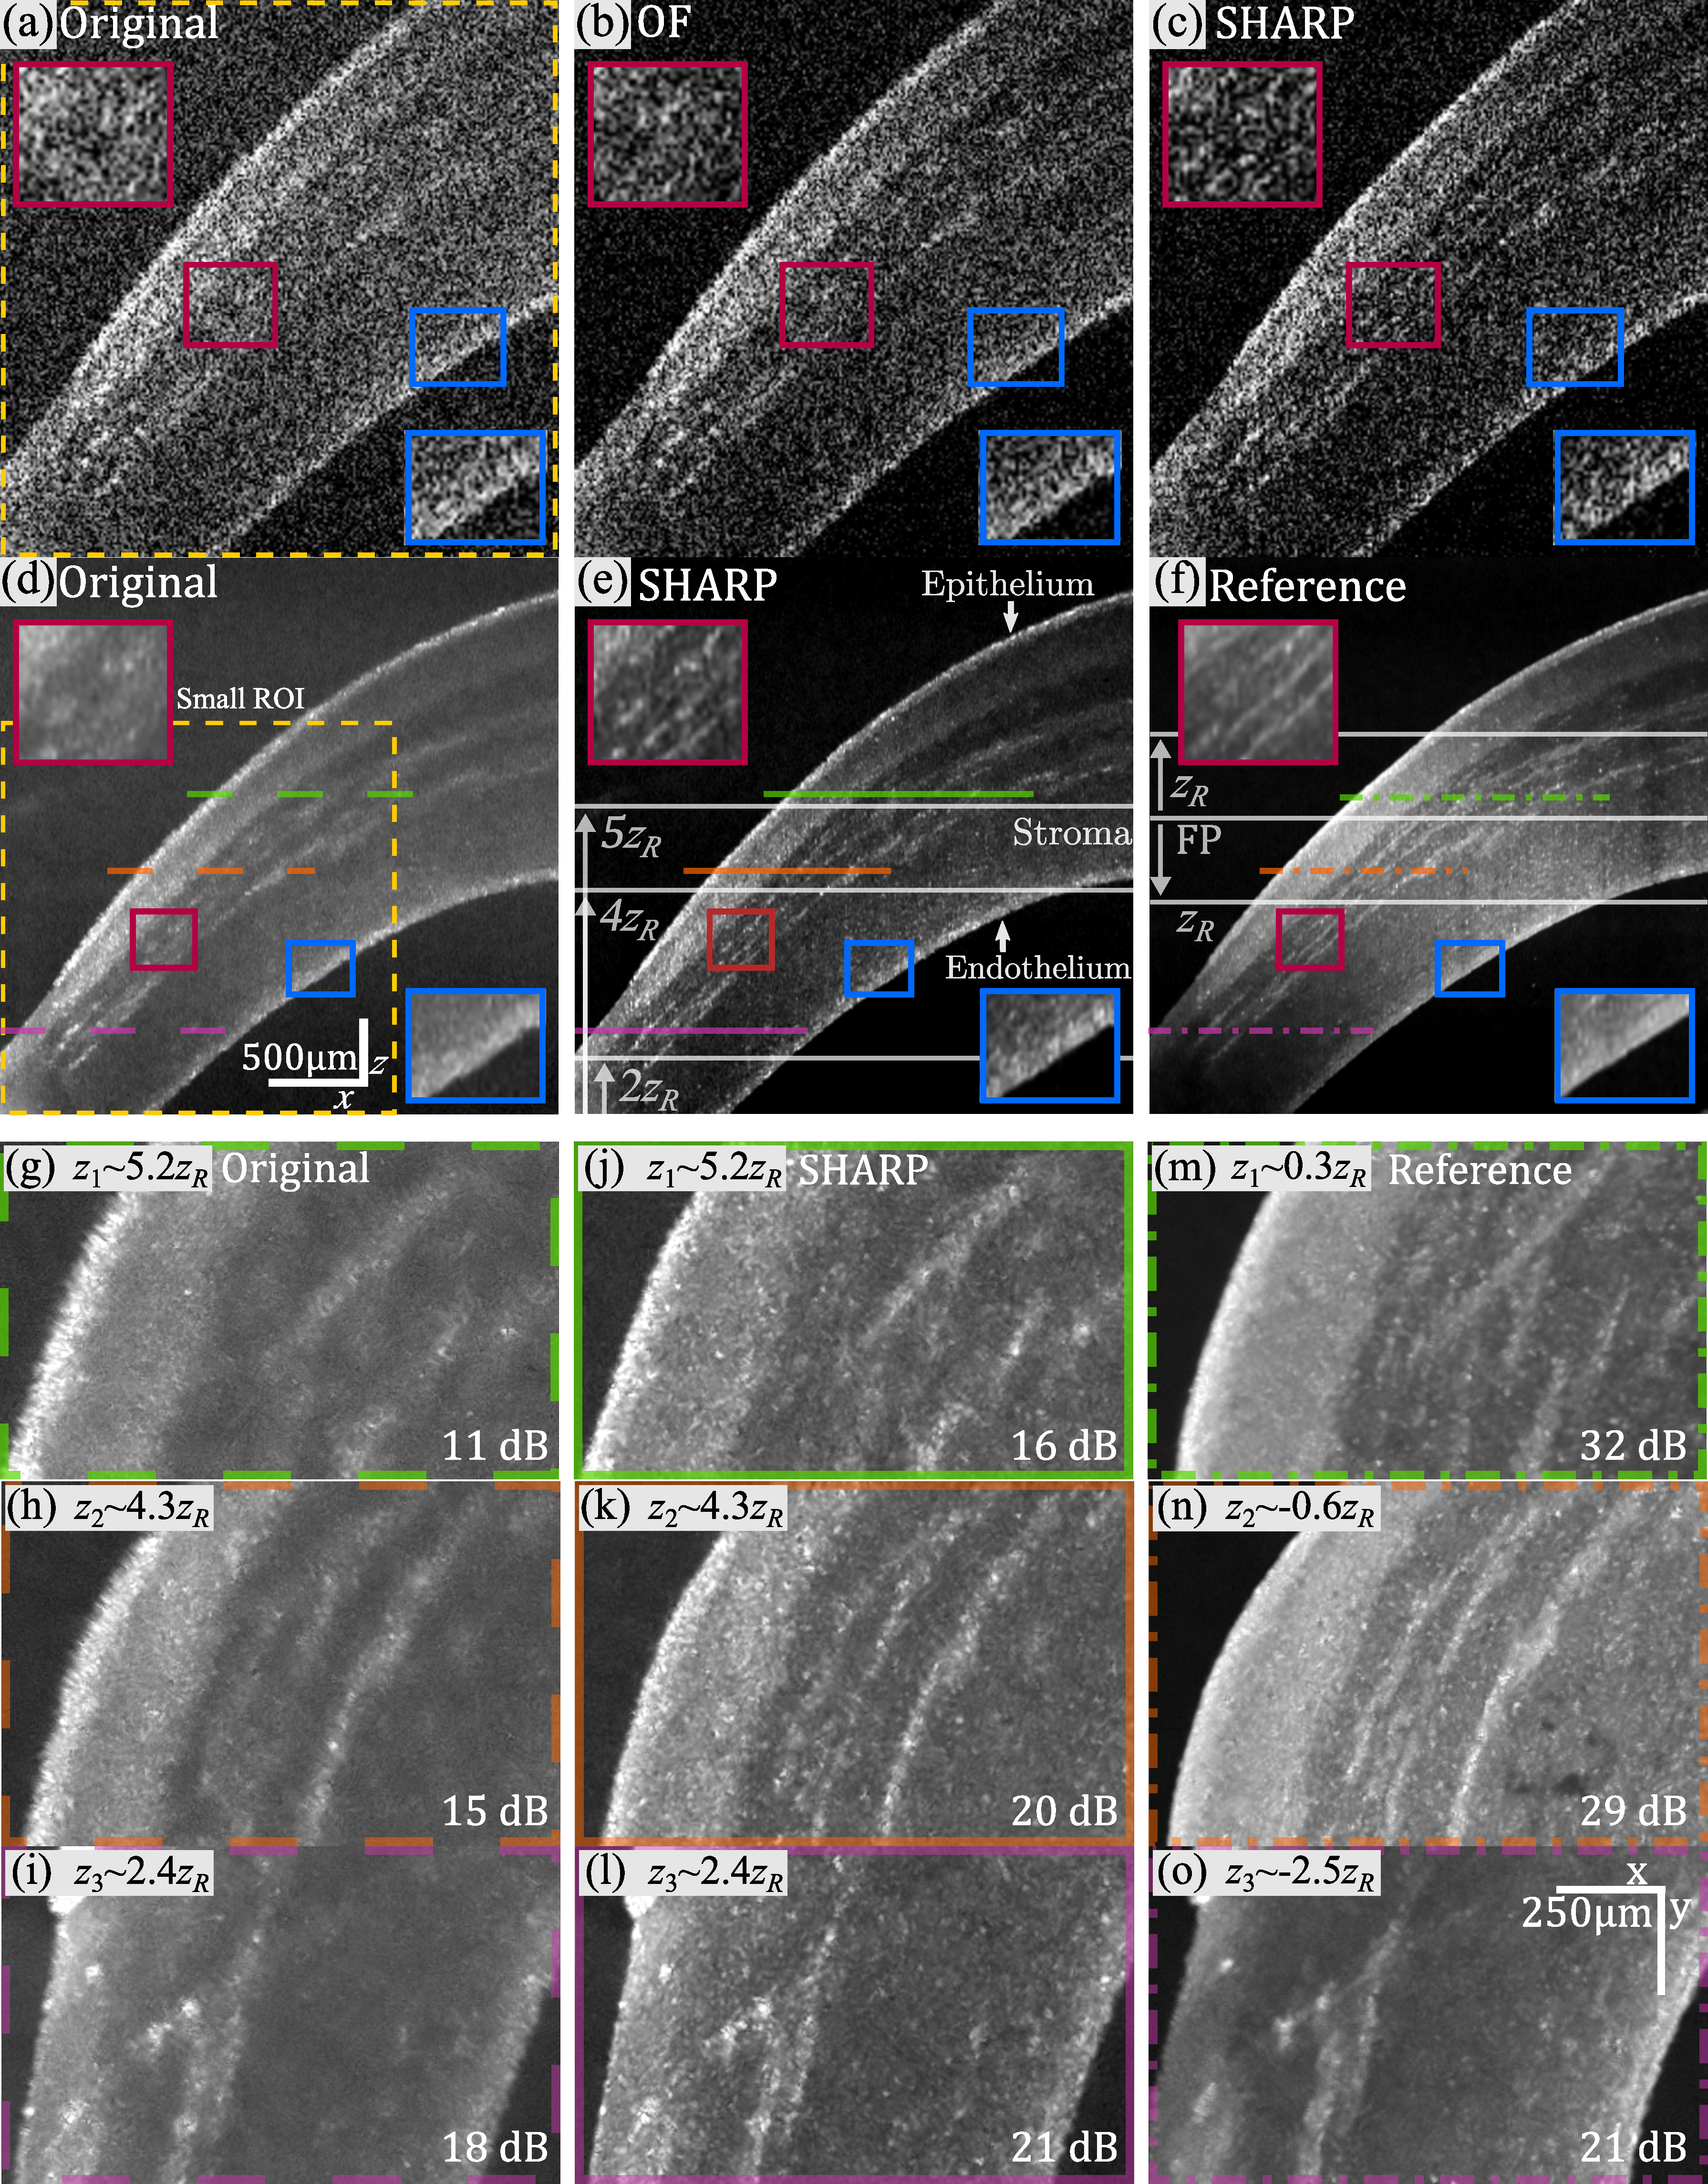
\includegraphics[width=\textwidth]{Figures/Results/ASImaging.pdf}
	\caption[Application of SHARP in anterior segment of excised swine eye.]{Application of SHARP in anterior segment of excised swine eye. Small ROI B-scans: (a) original, (b) optimum filter, and (c) SHARP. Full ROI B-scans after despeckling with TNode: (d) original, (e) SHARP and (f) reference (FP: focal plane, in (a)--(e) FP is in iris, out of image range). \textit{En face} at depths $z_i$ marked with lines in the B-scans: (g)--(i) original, (j)--(l) SHARP and (m)--(o) reference. Each \textit{en face} image shows its dynamic range.}
	\label{fig:ASImaging}
\end{figure}

Figures~\ref{fig:ASImaging}(g)--(o) show three despeckled \textit{en face} views of the original, SHARP and reference tomograms at three depths indicated by lines in Figs.~\ref{fig:ASImaging}(d)--(f). The dynamic range of each \textit{en face} view was adjusted to equalize the contrast for visual comparison. Blurring increases towards the cornea apex in the original views in Figs.~\ref{fig:ASImaging}(g)--(i). In contrast, SHARP views [Figs.~\ref{fig:ASImaging}(j)--(l)] have perceptually very similar resolution at all depths, enabling improved visualization of structures inside the stroma and clearer boundaries of the corneal epithelium, resembling reference images Figs.~\ref{fig:ASImaging}(o)--(m). These results show that SHARP could enable the examination of the iris and the full cornea in a single-shot acquisition with higher lateral resolution than currently possible, facilitating the accurate determination of parameters of clinical interest such as the stromal demarcation line and tissue layer thicknesses with existing OCT systems without regard to phase noise. Finally, the combination of SHARP and TNode provided a significant improvement of image quality compared to the original tomogram, in terms of resolution improvement, noise reduction and contrast.

\subsection{CTNode in combination with SHARP}

Back-scattering of cornea is relatively low because its constitutive tissue is inherently translucent for functional purposes, making that cornea stroma generally exhibits low to medium SNR, even lower in the presence of aberrations. In the previous demonstration of SHARP, the optimum filter shown to be a key tool to improve visualization of results in terms of noise suppression, providing an extended dynamic range. The aim now is to combine CTNode with SHARP to further improve contrast by reducing noise floor level.

After applying SHARP to the tomogram of previous demonstration, CTNode was applied using search and similarity windows of 11$\times$11$\times$11 and 3$\times$3$\times$3, respectively, and $h = 0.15$. Figure~\ref{fig:ASImaging_CTNode} shows a selected B-scan of the original tomogram, after SHARP and after subsequent CTNode. The upper value of the dynamic range of all images is the same but the lower limits were equalized to the noise floor level ($\mu_N$) of each image, computed as the average intensity within the blue rectangles in Figs.~\ref{fig:ASImaging_CTNode}(a)-(c), in order to match the visual contrast at the cost of having different dynamic ranges. More specifically, original B-scan in Fig.~\ref{fig:ASImaging_CTNode}(a) has a noise floor level of 56~dB and a dynamic range of $16$~dB, in SHARP B-scan in Fig.~\ref{fig:ASImaging_CTNode}(b) the noise floor was reduced by 6~dB, allowing to incraese dynamic range to 22~dB and after CTNode noise floor was additionally reduced by 5~dB, for a total reduction of 11~dB, allowing to increase dynamic range to 27~dB.

\begin{figure}[htb!]
	\centering
	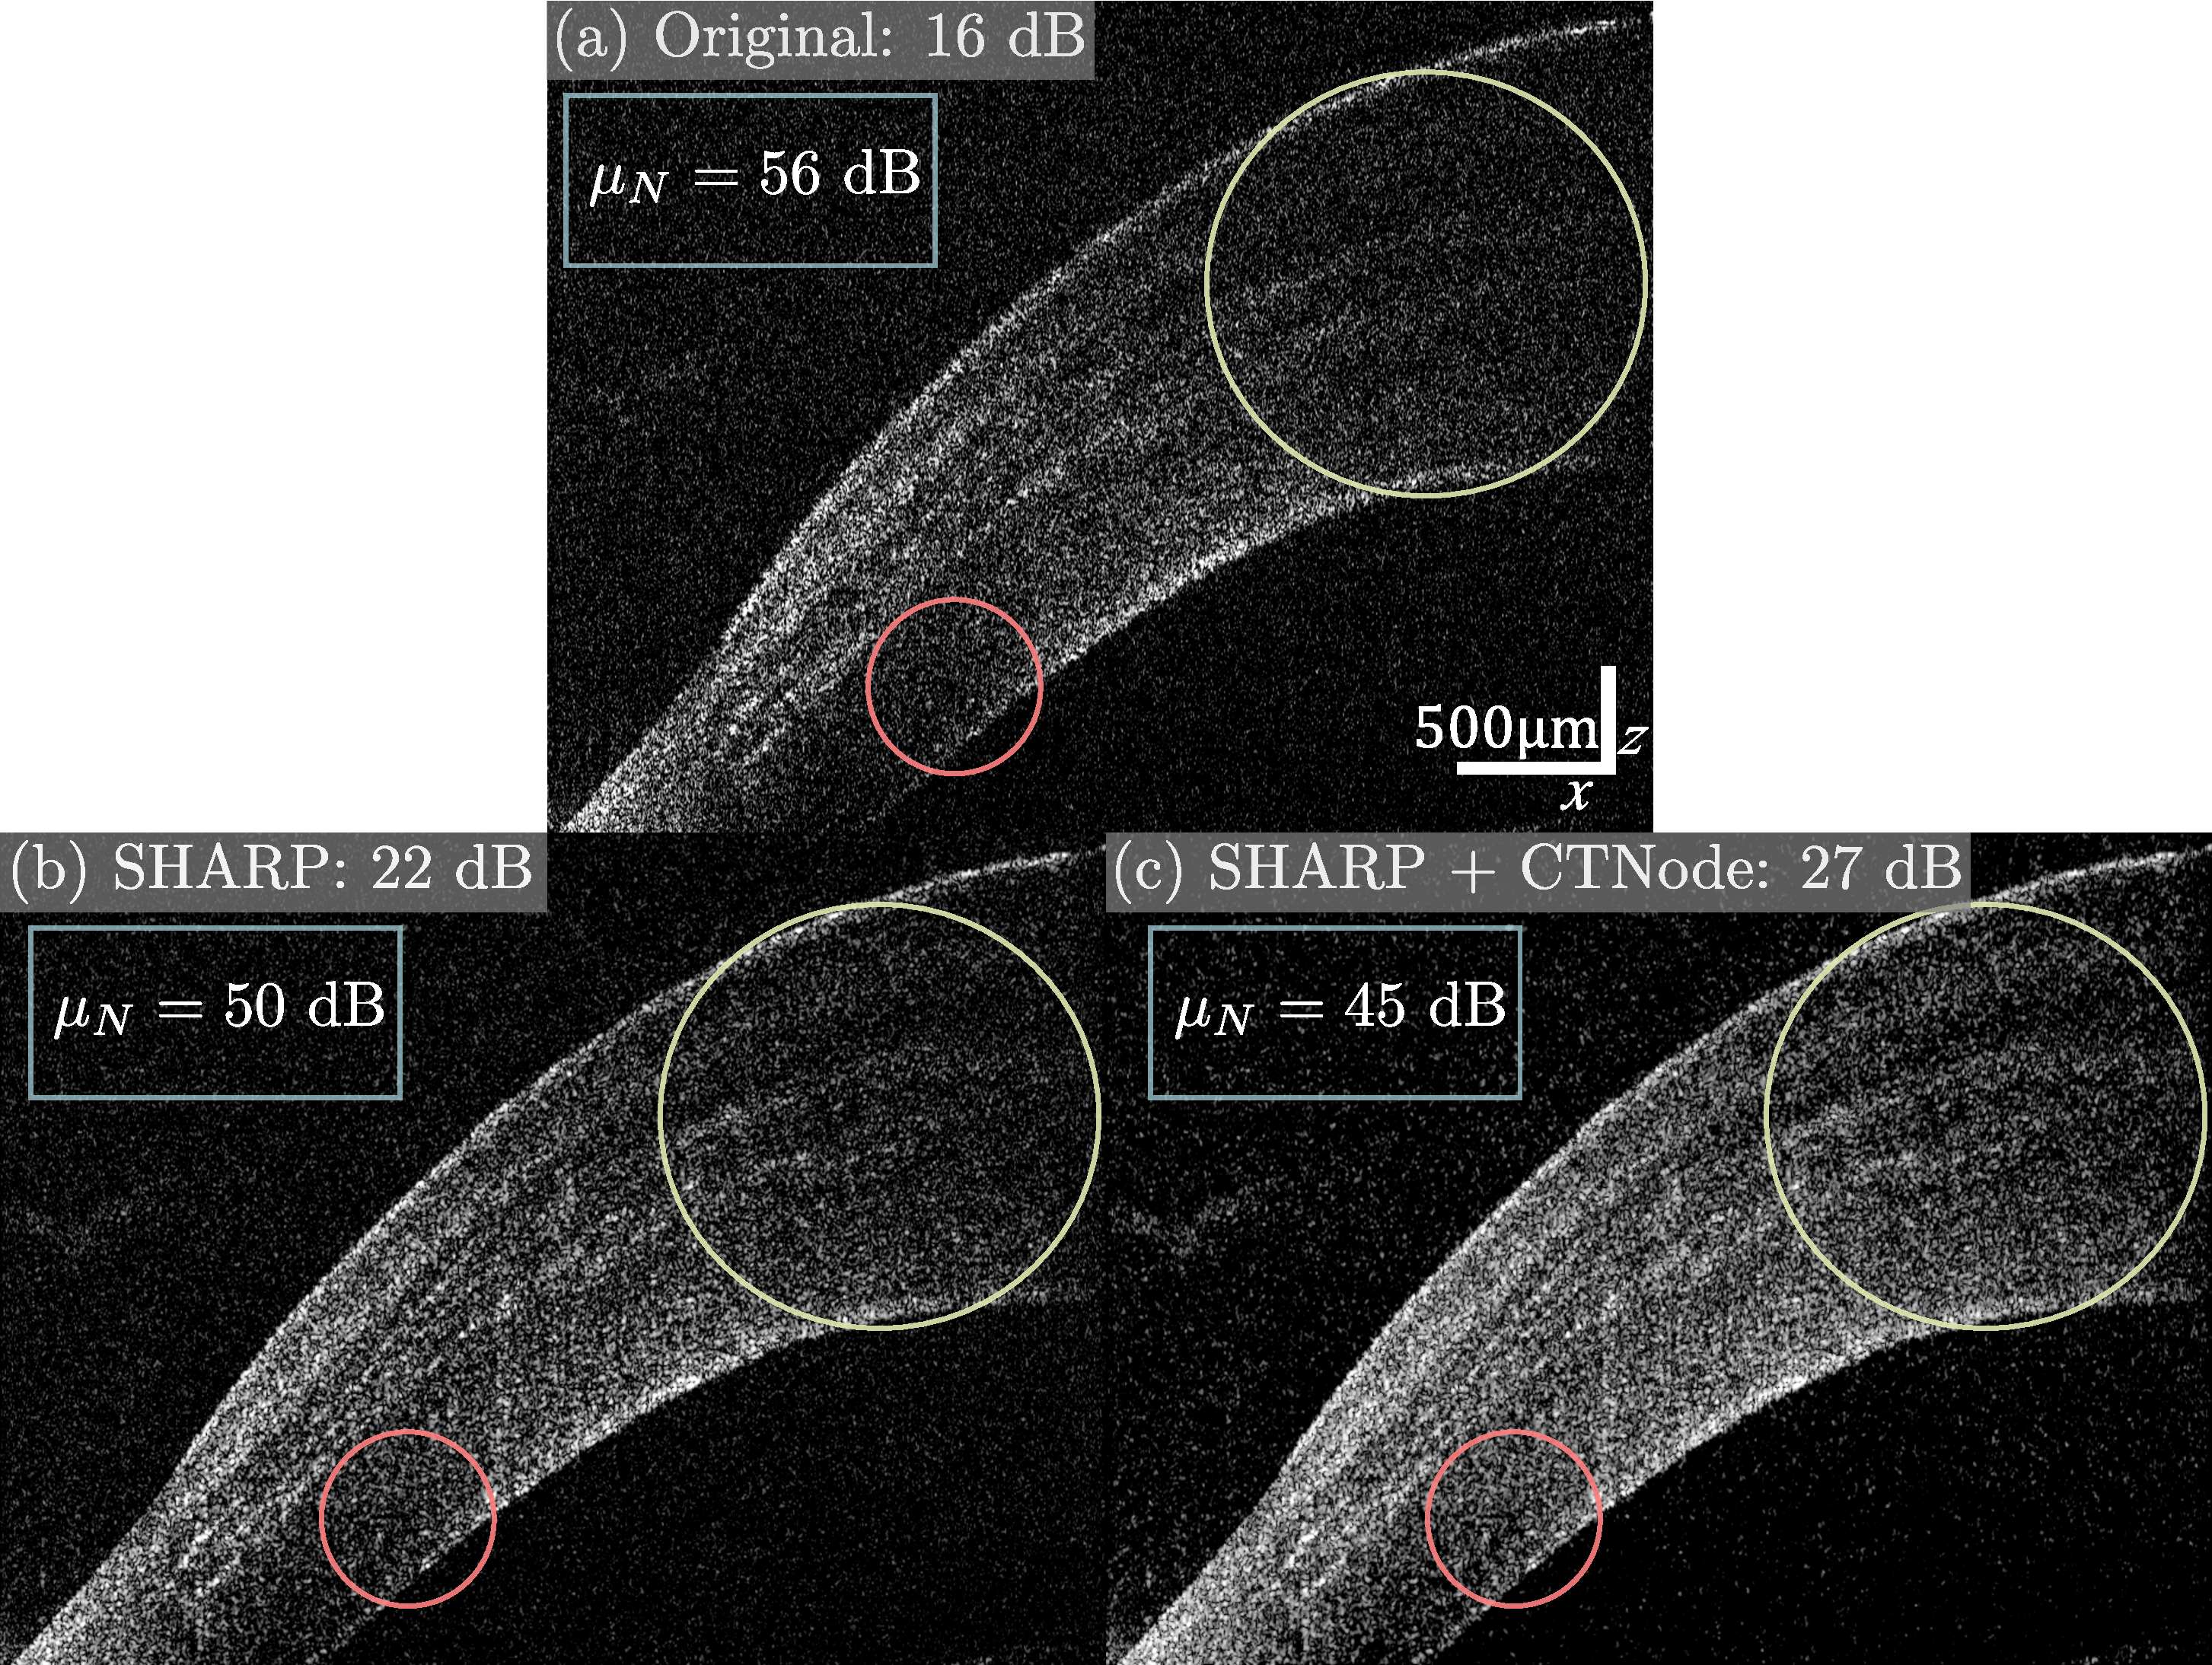
\includegraphics[width=\textwidth]{Figures/Results/ASImaging-CTNode.pdf}
	\caption[Combination of SHARP and CTNode in anterior segment of excised swine eye.]{Combination of SHARP and CTNode in anterior segment of excised swine eye. B-scan images: (a) original, (b) after SHARP and (c) after subsequent CTNode. Number in the label of each image corresponds to its dyanmic range.}
	\label{fig:ASImaging_CTNode}
\end{figure}

Apart from the correction of defocus, the image after SHARP and CTNode presents an overall improvement in contrast of low- and medium-SNR regions, such as the regions enclosed in circles of Fig.~\ref{fig:ASImaging_CTNode}(c) where signal is more clearly visualized than in their counterparts in Figs.~\ref{fig:ASImaging_CTNode}(a) and (b). A notable side effect is that contrast of high intensity signal seems to be reduced, as a consequence of the asymmetric extension of dynamic range: the noise floor level is decreased but the signal strength is not increased, but in fact it is technically impossible to increase signal strength computationally. Despite that, the beneficial effect of noise reduction is more significant, for instance the corneal stroma, presents a better contrast after CTNode than in the original image where stroma exhibits a signal just above noise floor level because of its relative low back-scattering and the negative effect of aberrations. This suggests that CTNode has potential to improve the visualization of tissue with low to medium SNR signal by means of noise reduction. Another important aspect is that no resolution loss was observed after CTNode, which is particularly relevant for SHARP given that it is desired to maintain the resolution improvement provided by correction of aberrations.

\FloatBarrier

\subsection{Correction of anisotropic defocus in the cornea}\label{sec:CorneaImaging}

The optical properties of the tissue being imaged affect the propagation of the probe beam, and in particular this may give rise to spatial variations of the focal position which means that the focus does not follow a plane but a deformed surface, depending on sample geometry. The cornea possess a curved surface and an index of refraction different to air and these features combined produce a variation of focal position across the field of view following a smooth curvature, resulting in a \textit{focal curve} rather than a focal plane. This phenomenon, encountered mainly in high-NA systems, demands spatially-varying aberrations correction.

To demonstrate correction of anisotropic defocus in the cornea, the SSOCT system was equipped with a scan lens producing an effective $e^{-2}$ beam diameter of 9~$\mu$m in a Rayleigh range of 97~$\mu$m. The excised swine eye was imaged around the cornea apex, tilting the sample to avoid signal saturation due to specular reflection near to the apex, which ultimately resulted in a even greater spatial variation of focal position. An ROI of 350 samples per A-lines, 1536 A-lines per B-scan and 1024 B-scans was selected, covering a lateral field of view of 5$\times$3.3~mm$^2$ in an axial ranging of 2~mm in air. It has been found that a better aberration correction is obtained if window-based CAO is applied after global CAO in each 1D aberration correction step, possibly because global correction serves as an initial estimate to aberration correction which is then improved locally with window-based correction. In this case, only Legendre polynomial $P_2$ was employed and, for window-based SHARP, the window size was set to 128$\times$128~px$^2$ (0.4$\times$0.4~mm$^2$)

\begin{figure}[b!]
	\centering
	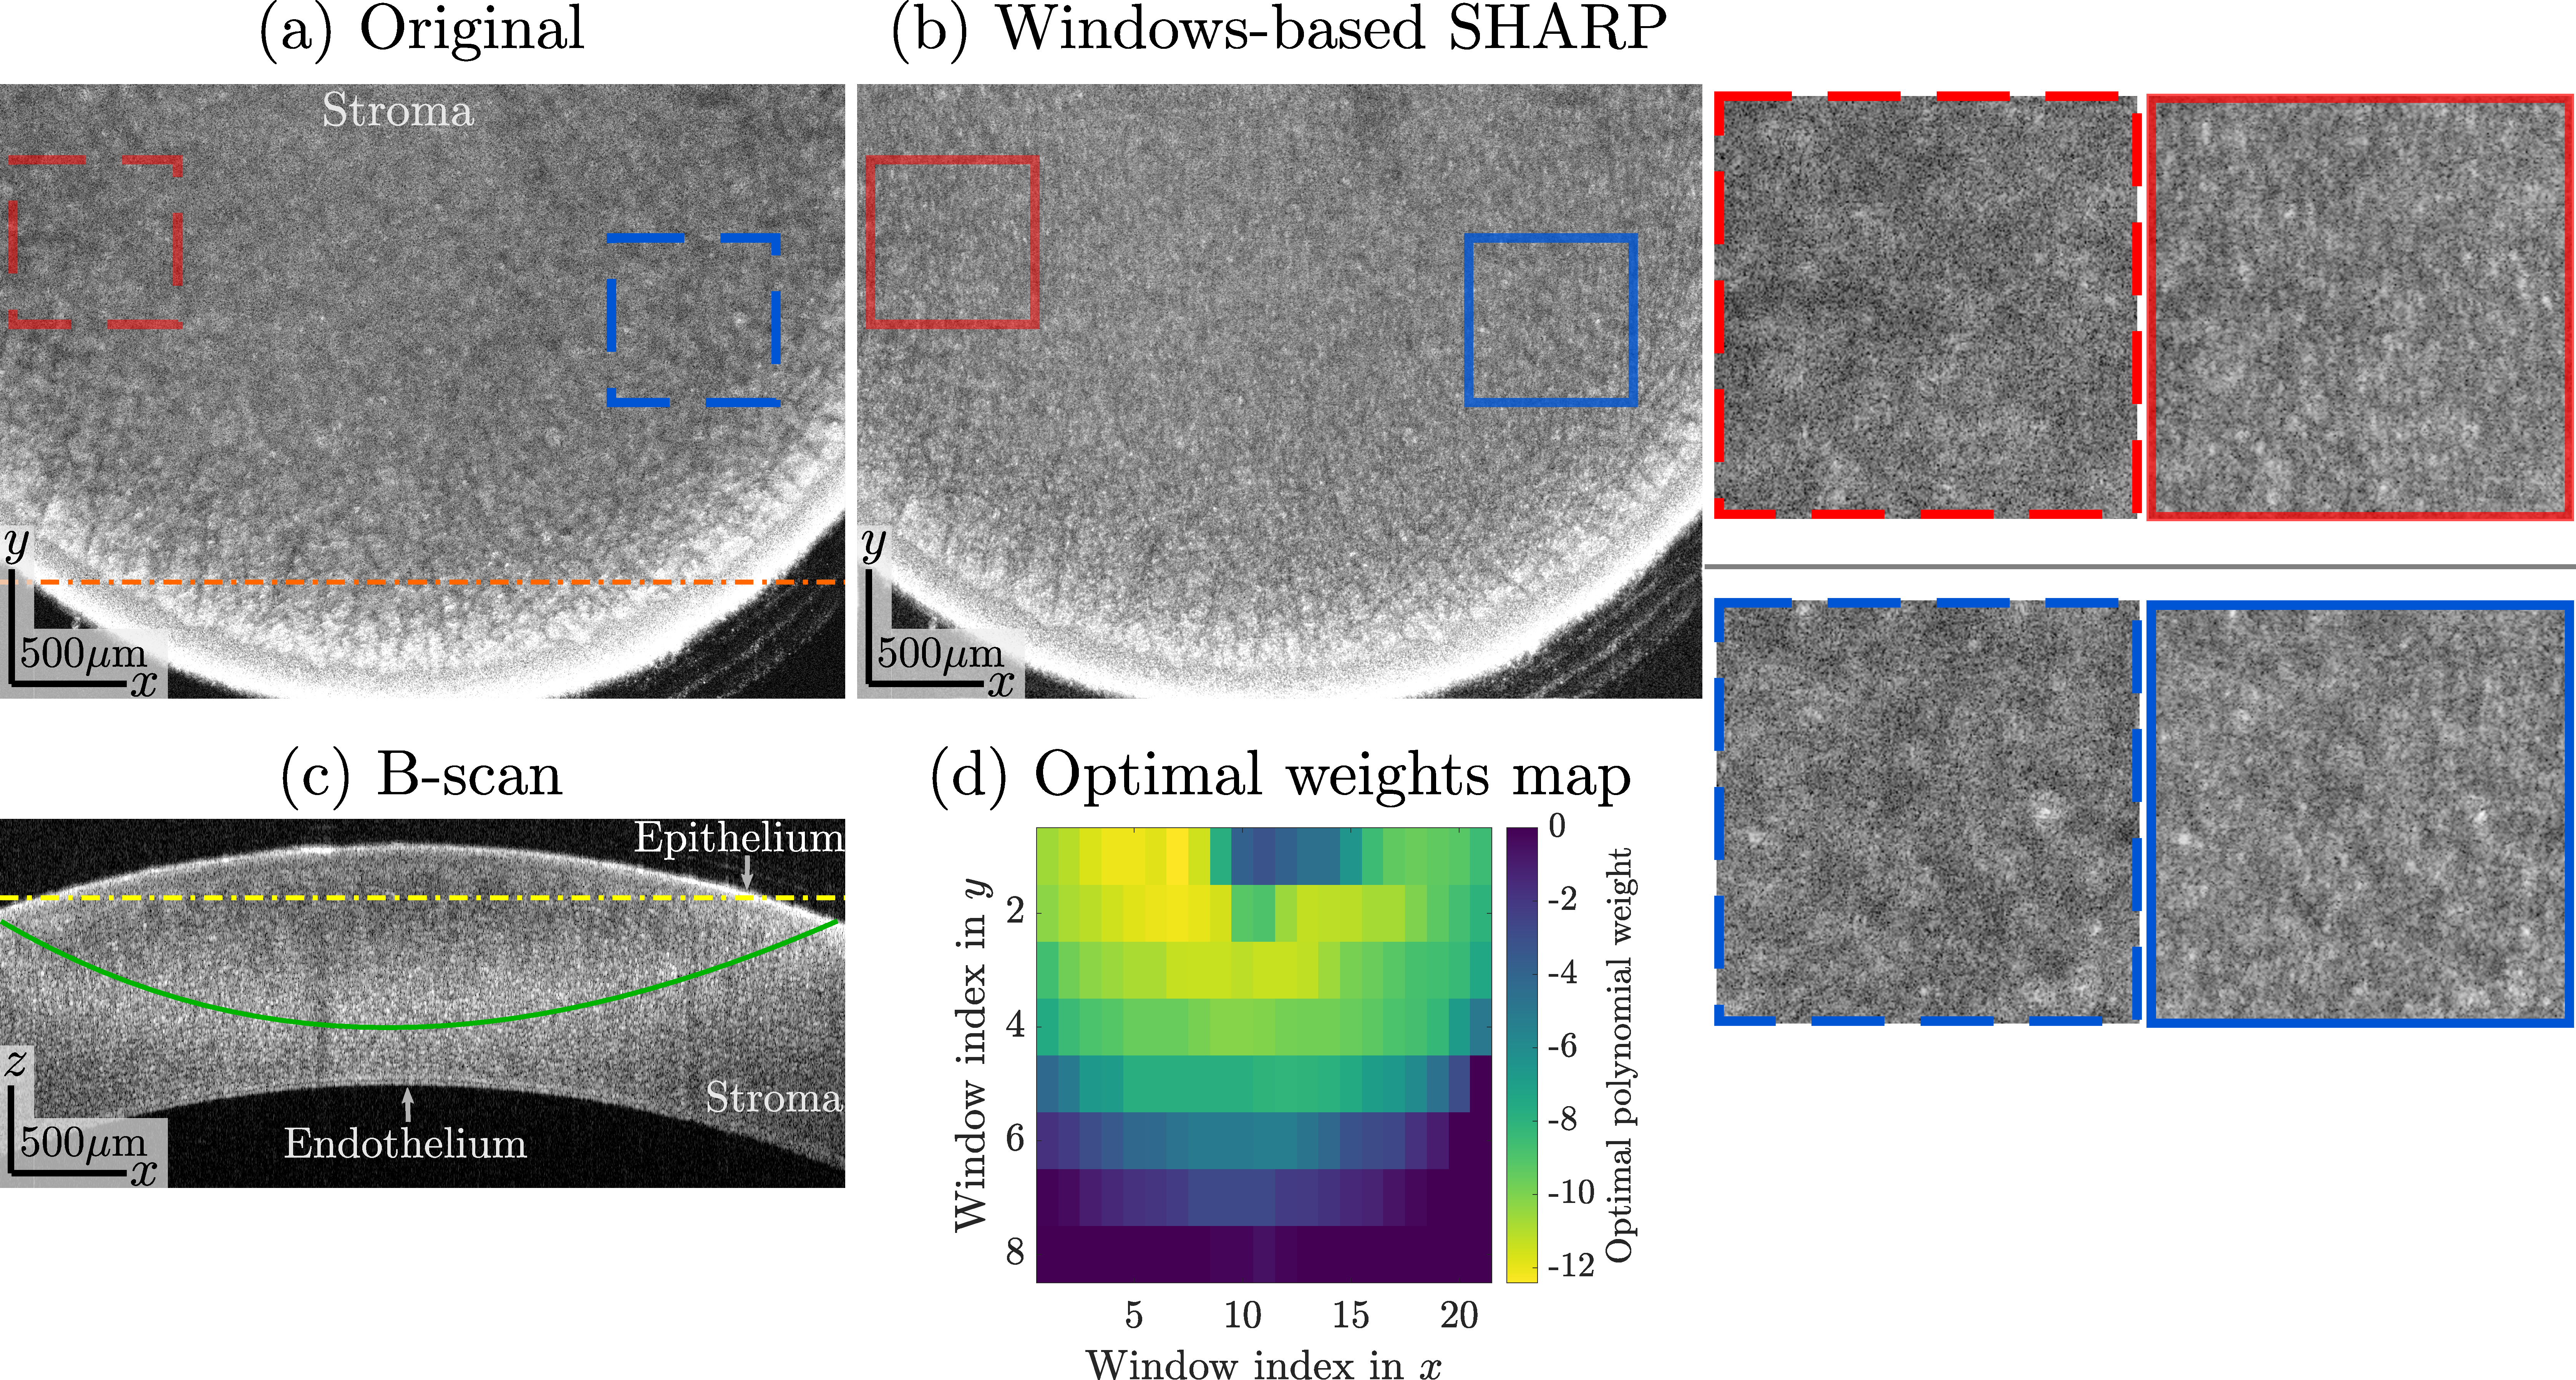
\includegraphics[width=\textwidth]{Figures/Results/CorneaImaging.pdf}
	\caption[Application of SHARP in cornea of excised swine eye.]{Application of SHARP in cornea of excised swine eye. \textit{En face} views: (a) original and (b) after global and window-based SHARP, located at depth marked by yellow dashed line in the original B-scan in (c), that at the same time corresponds to the location marked by orange dashed line in (a). (d) Two-dimensional map of optimal 
	weights for all windows found for correction along $x$ of \textit{en face} plane in (b).}
	\label{fig:ConrealImaging}
\end{figure}

Figure~\ref{fig:ConrealImaging} shows an \textit{en face} view of the original tomogram and after correction of aberrations with global and window-based SHARP. In this case, the optimum filter reduced noise floor level by 6~dB but contrast improvement is not evident because the dynamic range of original image in Fig.~\ref{fig:ConrealImaging}(a) was adjusted to match the contrast of the SHARP image in Fig.~\ref{fig:ConrealImaging}(b) for comparison purposes. Displayed \textit{en face} planes are located at a depth within the corneal stroma, marked by yellow line in original B-scan image in Fig.~\ref{fig:ConrealImaging}(c), presenting very dense signal but also fine structures that are significantly blurred in the original tomogram, whereas after SHARP they appear sharper given the improvement of lateral resolution, as noted when comparing the insets that show zoomed regions of the images.

In practical terms, the depth of field can be often identified in cross-sectional views as a bright intensity band because signal inside the depth of field is intrinsically stronger than outside. This way, it is possible to roughly determine the position of the focus as the center of this bright band, which in the B-scan view of Fig.~\ref{fig:ConrealImaging}(c) follows a curve instead of a plane, as marked by green line, indicating that indeed the location of the focus varies with lateral position, resulting in a focal curve. This effect can be also inferred from the two-dimensional map in Fig.~\ref{fig:ConrealImaging}(d) that shows the optimal weights determined for each window for the \textit{en face} plane in Fig.~\ref{fig:ConrealImaging}(b), which resemble the cornea curvature, instead of being constant across all windows as expected if the correction were purely global.

\FloatBarrier

\section{Complex noise reduction in human posterior segment imaging \textit{in vivo}}

Posterior segment of the eye is rich in structures that support the normal operation of the eye, such as the retinal nerve fiber layer, the photoreceptors layer and the choroid~\cite{Drexler2015_Retinal}. In general, these structures present high back-scattering that vary between them allowing a readily visual identification in intensity-contrast image. However, choroid and sclera typically present a lower signal, specially the sclera, given that they are at deep depths where signal strength is greatly affected by tissue absorption and the high reflectance of precedent layers like the retinal pigment epithelium. Measurement of the choroid thickness has been of great interest for diagnosis and study of pathologies~\cite{Yiu2014_Characterization}, and this requires to identify the choroid/sclera (C/S) junction in order to reliable identify the choroid and measure its thickness, but this task is difficult given the relatively low contrast of the C/S junction. 

An additional experimental validation of CTNode was performed, aiming to reduce noise in retinal imaging to improve contrast of structures, including the C/S junction. The posterior segment of a healthy subject was imaged using a retinal system described in~\cite{Braaf2018_Complex}. This SSOCT system is based on a VCSEL wavelength-swept source (Axsun Technologies, Inc., MA, USA) with an A-line repetition rate of 100~kHz and a spectral bandwidth of 91~nm centered at wavelength 1040~nm for an axial resolution of 10~$\mu$m in air. The system has a modified commercial ophthalmic interface (Heidelberg Engineering, Germany), that provides a diffraction-limited spot-size of 18~$\mu$m on the retina, with an integrated scanning laser ophthalmoscope (SLO) to track motion of the subject's eye by analyzing motion-induced affine image transformations compared to a pre-acquired reference SLO image, and then motion correction is translated to the control wave-forms of the galvanometers scanners of the SSOCT system on-the-fly in order to follow eye motions during the acquisition. Additionally, a reference reflection in a separated arm of the sample arm is available for 2D phase stabilization.

The acquired tomogram consisted in 2048 depth samples, 1024 A-lines per B-scan and 1024 B-scans, from which an ROI of 820$\times$960$\times$768 was extracted for processing. Phase was stabilized using the reference reflection~\cite{Vakoc2005_Phaseresolved}. Furthermore, residual motion was observed despite the use of the motion tracking system, mostly slow-frequency motion, that was corrected using intra-B-scan bulk motion correction as described in Section~\ref{sec:MotionCor}. Phase stabilization and motion correction enabled the use of 3D search and similarly windows, which otherwise would be restricted to 2D or 3D with limited performance. CTNode was applied using search and similarity windows of size 15$\times$15$\times$15 and 3$\times$3$\times$3, respectively, and $h=0.12$.

B-scan views of the original tomogram and after CTNode are shown in Figures~\ref{fig:RetinalCTNode}(a) and (b), corresponding to the cross-section marked by red dashed lines in \textit{en face} views shown in Figs~\ref{fig:RetinalCTNode}(d) and (e). In the original image, signal decays smoothly in the choroid making it difficult to identify the C/S junction. Application of CTNode provided a noise level reduction of 6~dB, allowing to increase the dynamic range of the image from 38~dB to 44~dB. This improvement is visualized in the medium-SNR layers in between the retinal nerve fiber layer and the photoreceptors layer that present a high contrast with respect to noise floor level, but the contrast between layers seems to be reduced, due to the side-effect of CTNode mentioned before. Anyhow, the interest is not to visualize high intensity layers, but more importantly the signal in the choroid that is more clearly identified from the sclera which is masked by the noise level, and this could improve further determination of C/S junction. Plot in Fig.~\ref{fig:RetinalCTNode} shows A-line profiles of the original and CTNode tomogram, at location marked by blue dashed lines in Figs.~\ref{fig:RetinalCTNode}(a) and (b). Signal within the green line have high intensity and thus reduction of noise is inconsequential, but for low signal regions within the orange line, such as the sclera, noise reduction is perceived as a decrease in signal intensity. Finally, Figs.~\ref{fig:RetinalCTNode}(d) and (e) show \textit{en face} views of the original and CTNode tomograms at depths marked by purple dashed lines in the B-scans. Signal around the optic disc is very homogeneous in the original \textit{en face} because SNR is low and noise dominates, instead, CTNode \textit{en face} view displays a transition in signal intensity from the choroid to the sclera. 

\begin{figure}[htb!]
	\centering
	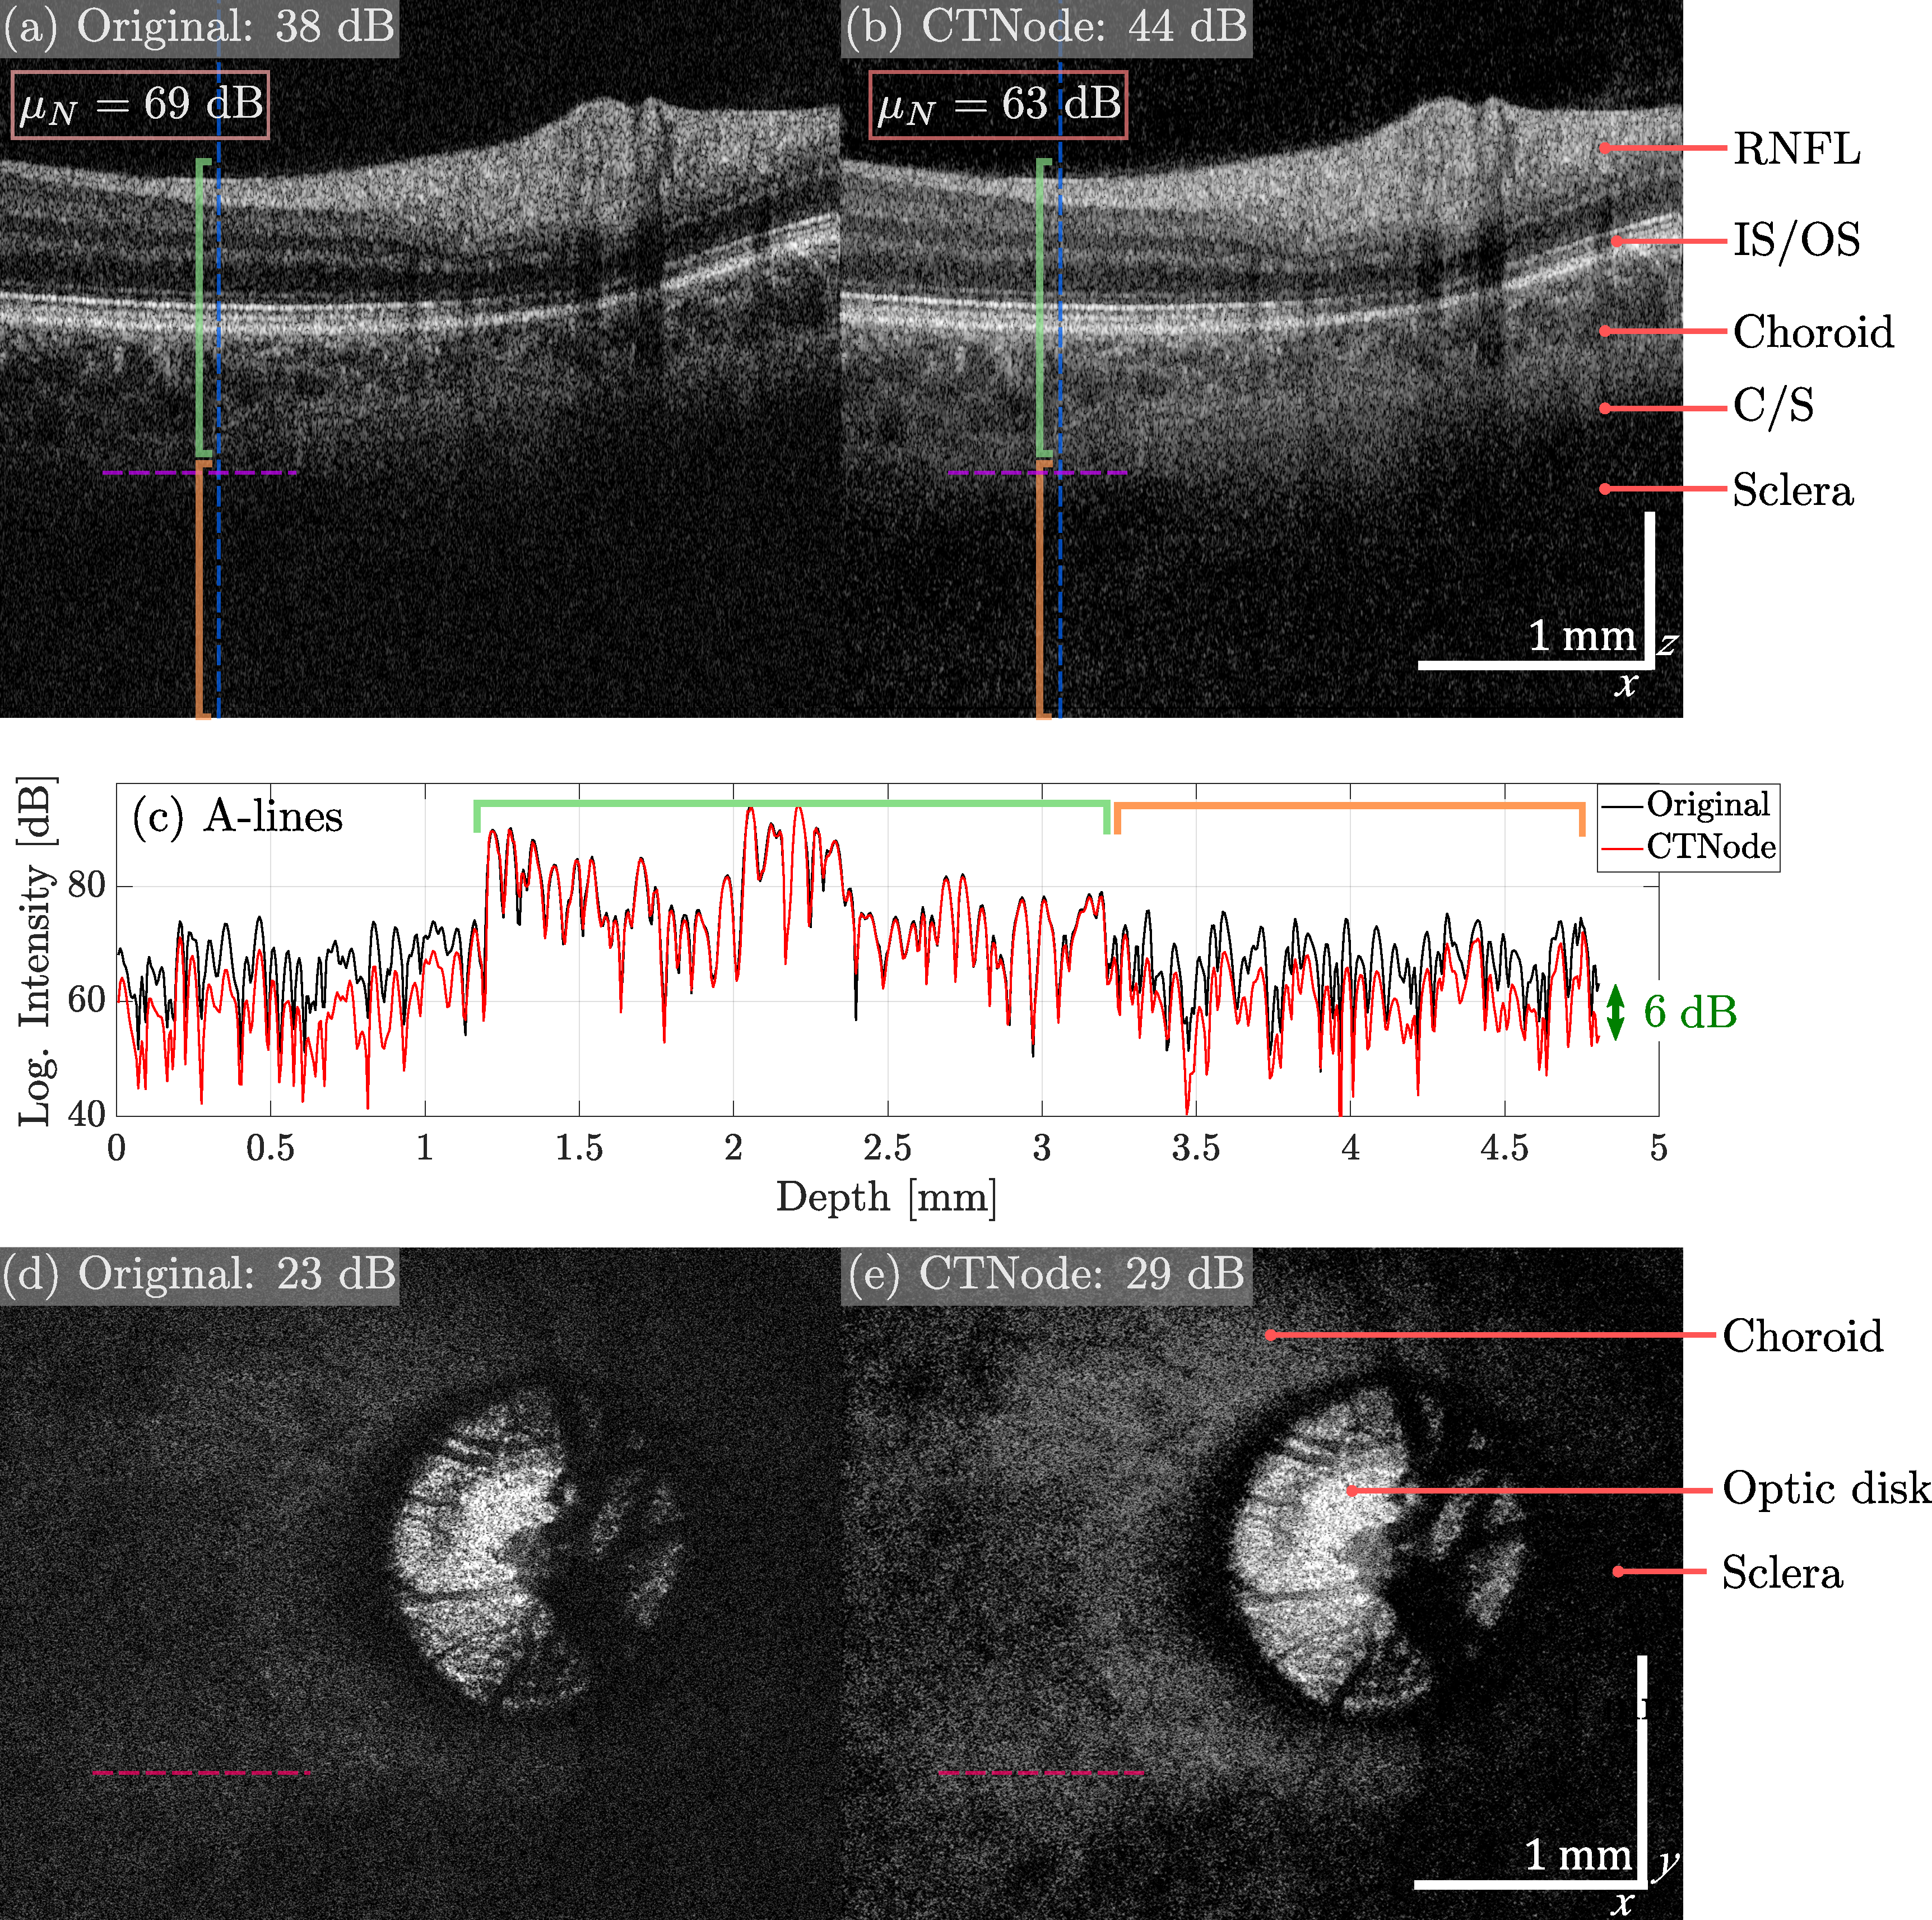
\includegraphics[width=\textwidth]{Figures/Results/RetinalCTNode.pdf}
	\caption[Reduction of noise with CTNode in retinal imaging \textit{in vivo}.]{Reduction of noise with CTNode in retinal imaging \textit{in vivo}. B-scan views: (a) original and (c) after CTNode, corresponding to the plane marked by red dashed lines in \textit{en face} views: (d) original and (e) after CTNode, at depth marked by purple dashes lines in (a) and (b). (c) A-line profile of original and CTNode tomograms at locations marked by blue lines in (a) and (b). RNFL: retinal nerve fiber layer, IS/OS: inner and outer photoreceptors segment junction, C/S: Choroid/sclera junction. }
	\label{fig:RetinalCTNode}
\end{figure}

\FloatBarrier

\section{Endoscopic imaging \textit{in vivo}}

To access internal tissue like coronary artery~\cite{Brezinski1996_Imaging} or gastrointestinal tract~\cite{Isenberg2003_Gastrointestinal} with endoscopic OCT, the scanner system composed of the galvo mirrors is replaced by a catheter that is inserted into the tissue lumen to guide light and to image internal structures. Light propagates inside the catheter through an optic fiber until the output tip, then it is focused by a gradient-index (GRIN) lens and finally it is reflected by a mirror or a prism by 90$^\circ$,  perpendicular to the lumen direction towards the interior of tissue~\cite{Hu2015_Optical}, as illustrated in Figure~\ref{fig:CatheterSchematic}. To scan the sample, A-lines are acquired while the catheter is being rotated by an external or internal actuator, providing B-scans of axial and \textit{azimuthal} axes, and additionally the catheter is pulled-back along the \textit{longitudinal} axis during the scanning to acquire multiple frames producing volumetric data. The probe is enclosed in a protective transparent tube to provide stability and prevent mechanical damage arising from the direct contact of the optics and the tissue, but this element induces astigmatism given its cylindrical geometry~\cite{Hu2015_Optical, Wang2012_Numerical, Xi2009_Highresolution}. As a consequence, the beam spot size in the longitudinal axis is different to that in the azimuthal axis, furthermore, the working distance in B-scan plane $d_x$ becomes larger than in longitudinal plane $d_y$~\cite{Wang2012_Numerical}, as depicted in Fig.~\ref{fig:CatheterSchematic}

\begin{figure}[htb!]
	\centering
	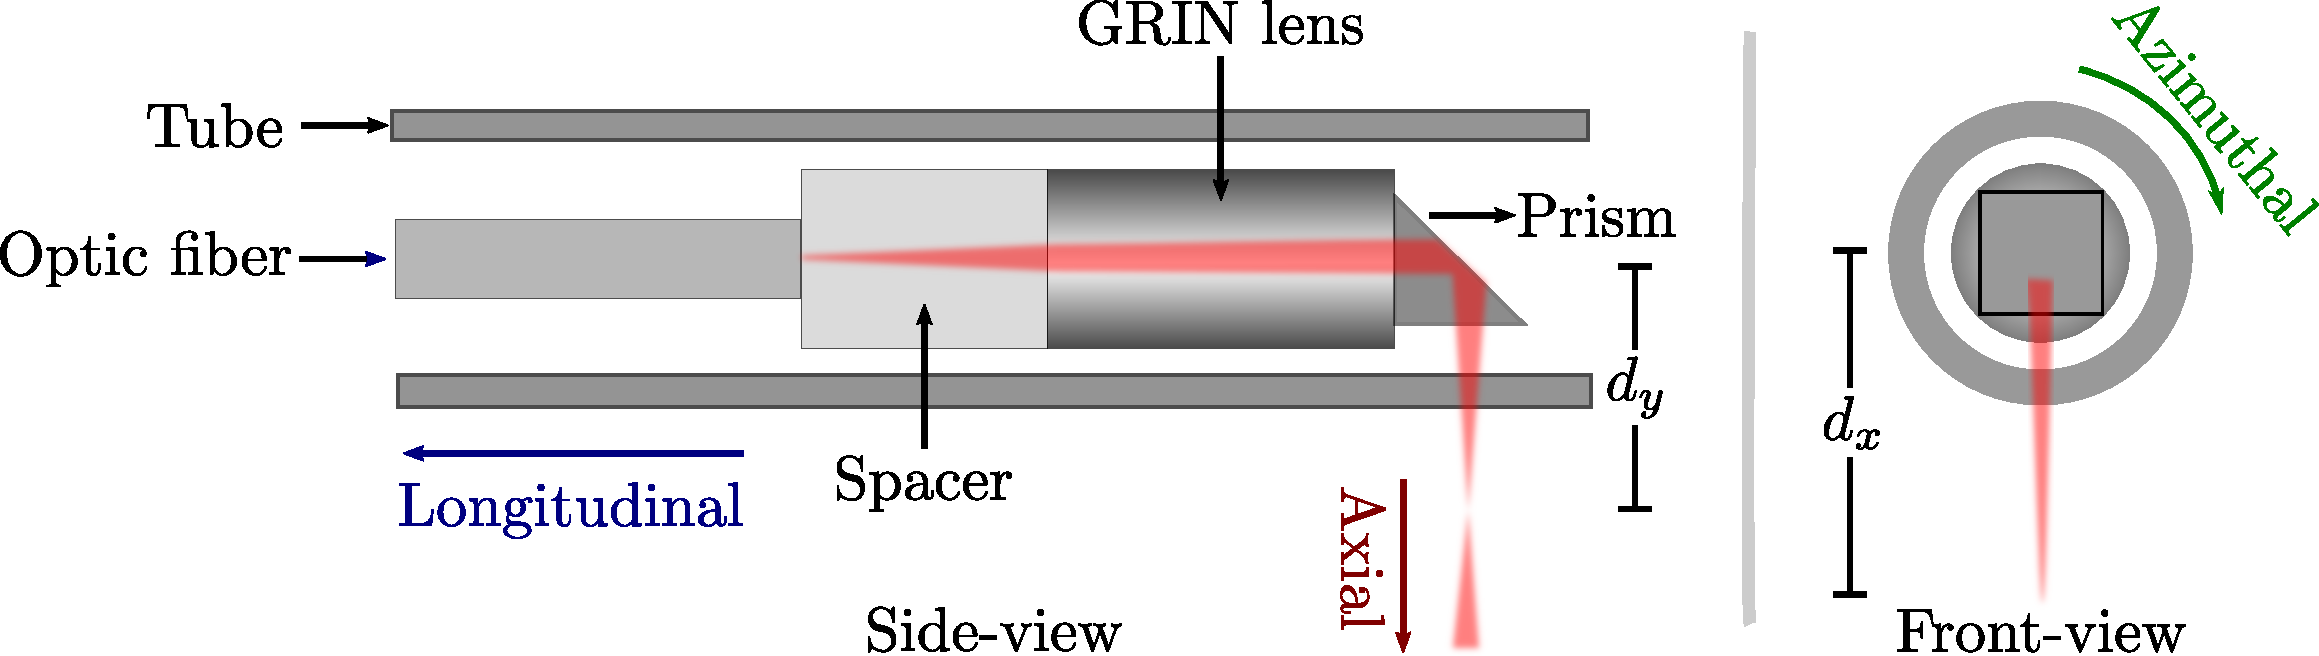
\includegraphics[width=.9\textwidth]{Figures/Results/CatheterSchematic.pdf}
	\caption[Schematic of a catheter for endoscopic OCT imaging.]{Schematic of the side and front view a catheter for OCT imaging.}
	\label{fig:CatheterSchematic}
\end{figure}

In raster scan systems, it is possible to adjust the distance between the scan lens and the sample to position the region of interest inside the imaging range, however, because the catheter-sample distance is fixed in endoscopic imaging, the working distance is a key feature in practical scenarios. For instance, a long working distance is required in esophageal imaging, whereas a short one is demanded in coronary artery imaging~\cite{Wang2012_Numerical}, thus optical design of catheter has become important~\cite{Hu2015_Optical, Xi2009_Highresolution, Kang2010_Endoscopically}, in order to produce astigmatism-free catheters with the desired working distance. Computational refocusing has the potential to facilitate optical design of catheters by correcting the negative effect of astigmatism and providing focused images across a larger depth of field without need of changing the working distance of the catheter.

The pullback of the catheter is typically performed such that the longitudinal sampling is often very sub-Nyquist and unevenly sampled, also, severe motion artifacts appear due to the probe rotation and the pullback, and for these reasons longitudinal axis is unsuitable for numerical aberration correction, thus only 1D refocusing is possible in endoscopic imaging, which is indeed possible with SHARP-$x$, computing only $\tilde{S}^{\text{1D}}$ in Eq.~\eqref{eq:SHARP}.

\begin{figure}[b!]
	\centering
	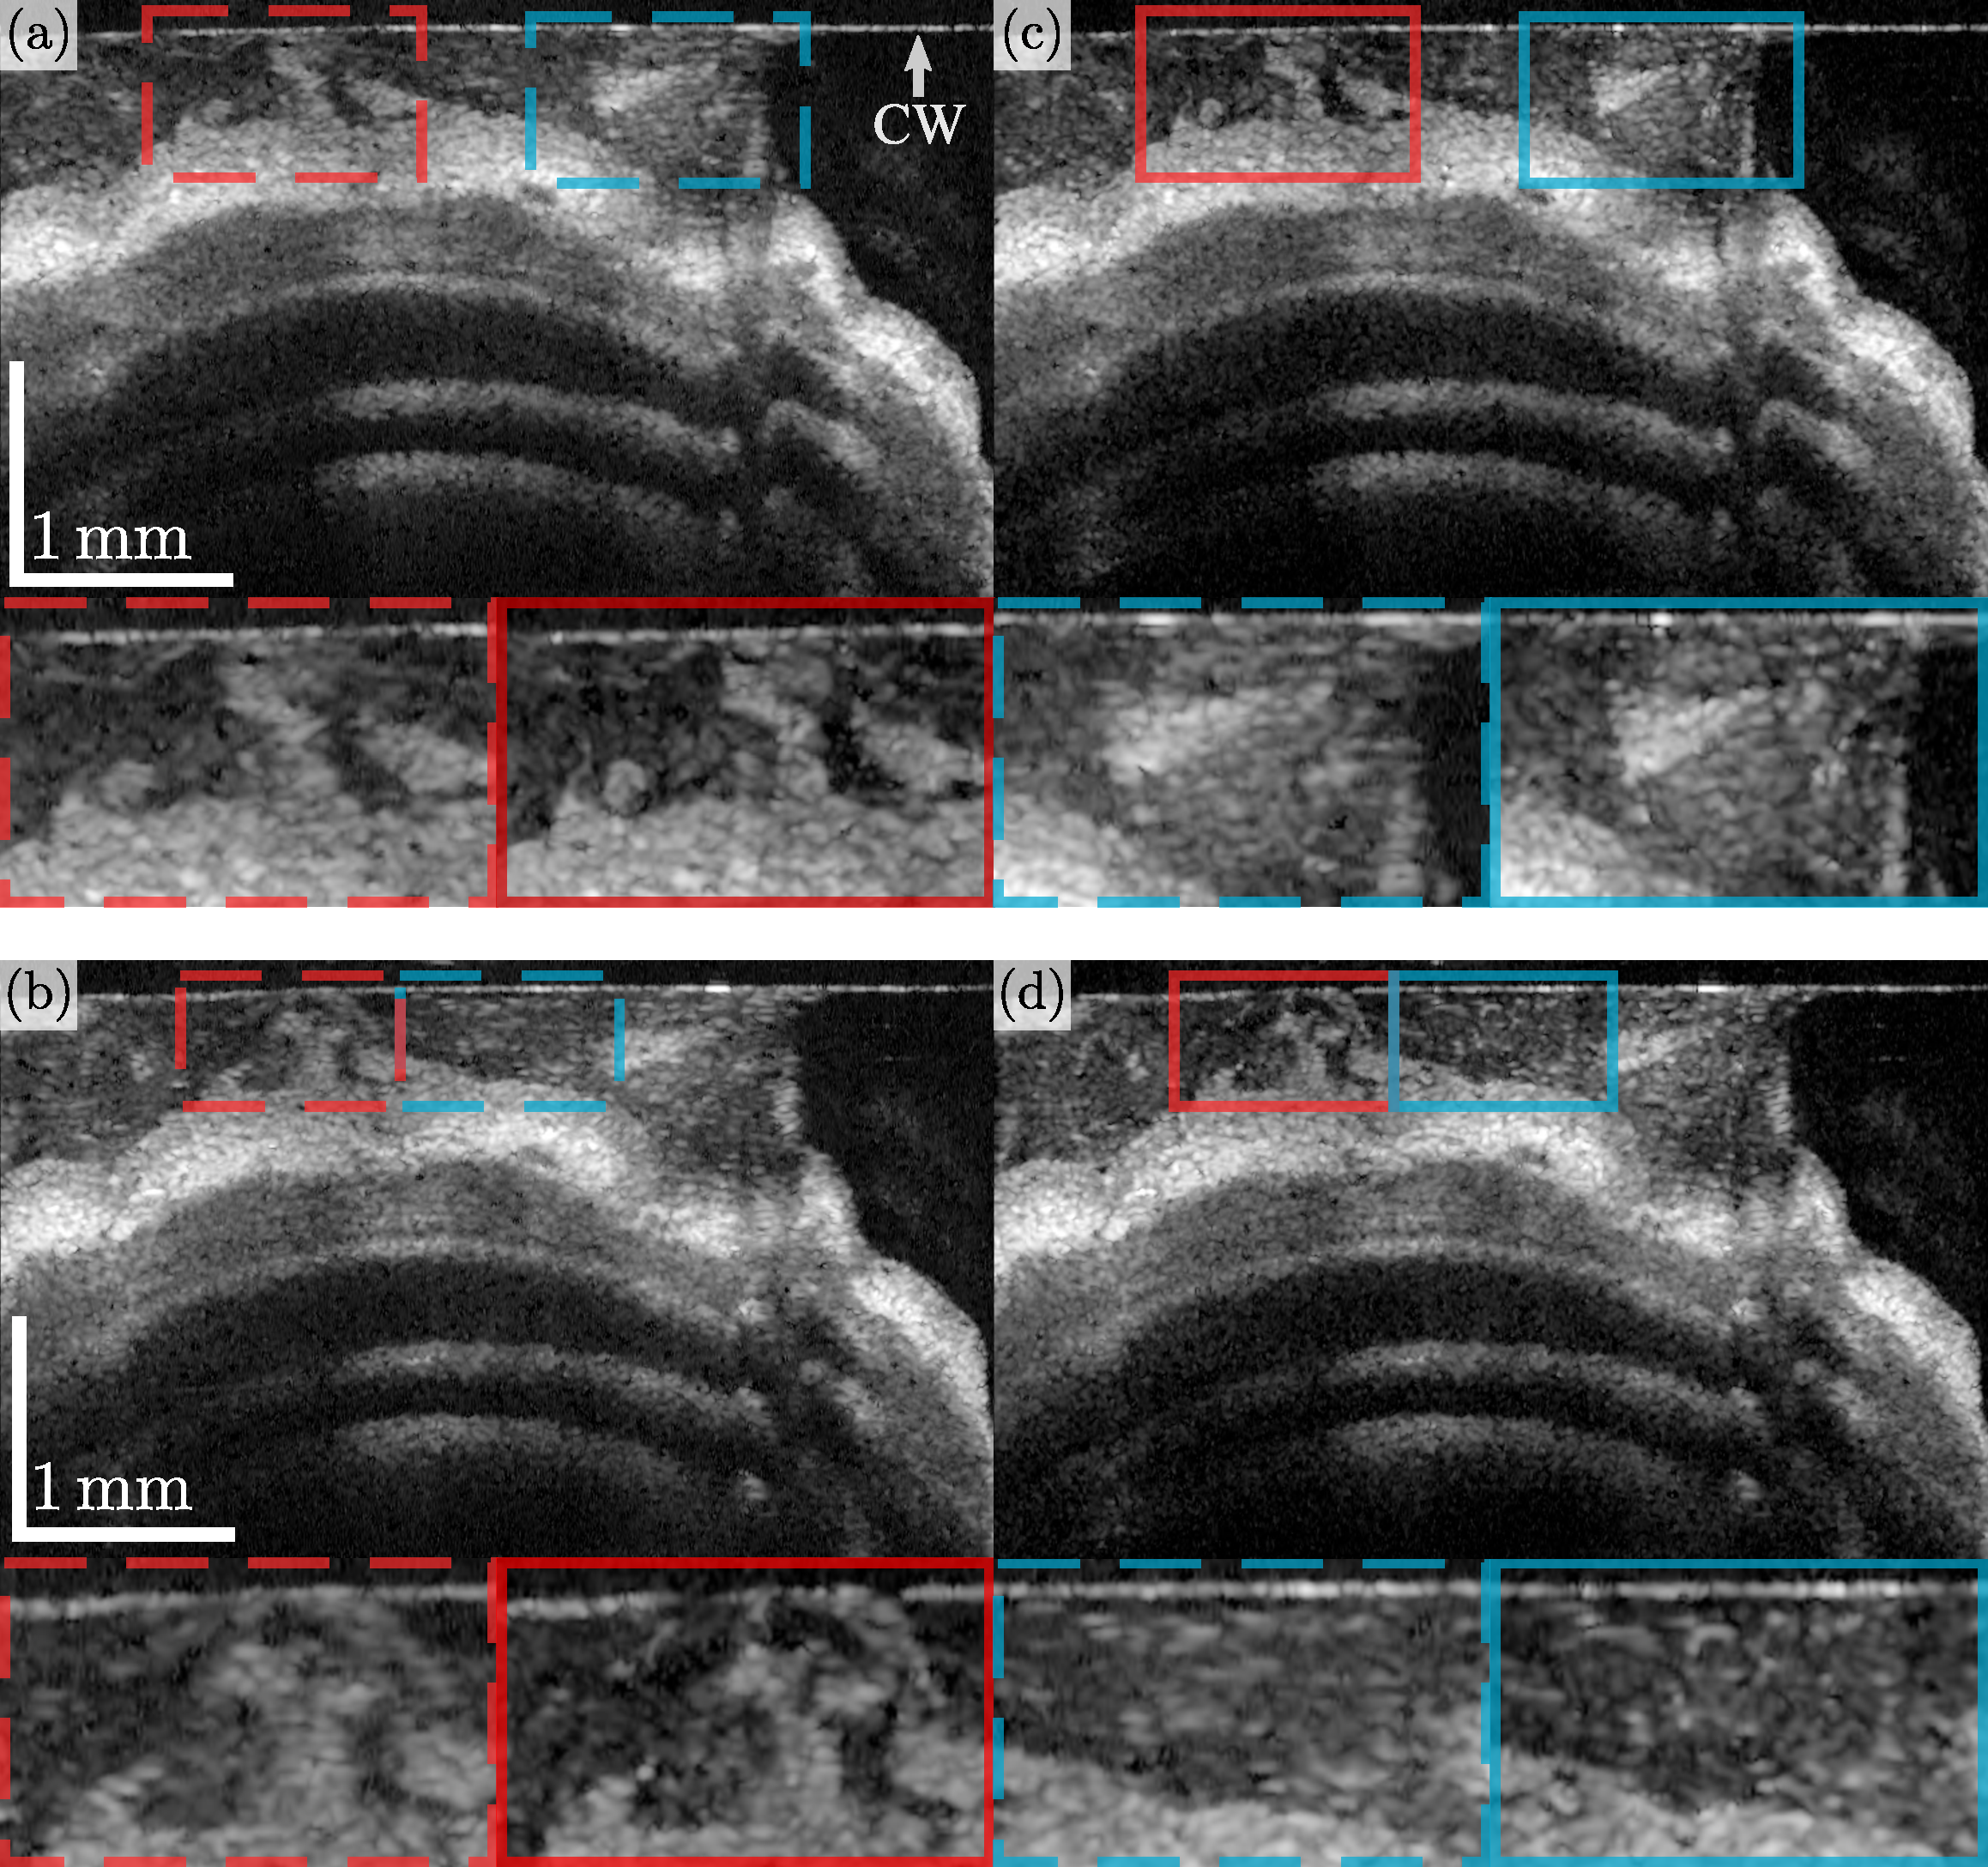
\includegraphics[width=.9\textwidth]{Figures/Results/CatheterImaging.pdf}
	\caption[Application of SHARP in endoscopic imaging of swine airway \textit{in vivo}.]{Application of SHARP in endoscopic imaging of swine airway \textit{in vivo}. B-scan views: (a)-(b) original and (c)-(d) SHARP-$x$. CW: catheter wall.}
	\label{fig:CatheterImaging}
\end{figure}

To demonstrate 1D operation of SHARP in endoscopic OCT for defocus and/or astigmatism correction, pullbacks of the airway of a swine were acquired \textit{in vivo} with a non-$k$-clocked catheter-based OCT system (NinePoint Medical Inc., Bedford, MA) having a 50~kHz polygon-based wavelength-swept source with $90$~nm $10$-dB bandwidth at central wavelength $1310$~nm and $e^{-2}$ beam diameter of $2w_0=40~\mu$m with Rayleigh range $z_R=1$~mm in air. SHARP was applied using $P_2$ only and TNode despeckling was performed afterwards using similarity and search windows of 5$\times$5$\times$0 and 31$\times$31$\times$5 pixels, respectively, and filtering parameters $h_0 = 0.06$ and $h_1 = 0.03$. Figure~\ref{fig:CatheterImaging} presents original and SHARP B-scans after TNode at two pullback positions showing an ROI of 450$\times$750~px$^2$ above the focal plane, which is located close to the lower edge of the images, making that structures near to the catheter wall appear blurred. Although 1D correction alone is more limited than 2D correction, SHARP-$x$ still provides an enhancement for depths $z>z_R$. In particular, debris in the mucus layer, located just below the catheter wall, is brought into focus as seen in the insets. This result suggests that SHARP-$x$ could improve endoscopic imaging when there is no fixed probe-tissue working distance, such as in airway and intravascular imaging, by combining long working distance catheters with SHARP to provide focal resolution in an extended range.

\section{Skin imaging \textit{in vivo}}

OCT offers readily observation of features of the skin such as stratum corneum, sweat ducts and dermal/epidermal junction and promises to offer key information for quick reliable diagnosis, in applications where avoiding skin biopsy is desirable~\cite{Holmes2015_OCT}.

To demonstrate operation of SHARP in skin imaging, a tomogram of a human hand dorsal surface was imaged \textit{in vivo} with the focal plane above the sample surface, using the same system and configuration used for the proof of concept experiment but selecting now an ROI of 500 samples per A-line, 512 A-lines per B-scan and 256 B-scans. The sample was imaged around the metacarpophalangeal joint, which presents an inhomogenous surface inducing spatial variations of defocus that make insufficient to correct the entire lateral FoV globally. Therefore, windows-based SHARP was applied using windows of size 64$\times$64~px$^2$. Although the hand of the subject was resting on a platform, small, low-frequency motion is evidenced in the tomogram, possibly dominated by heartbeat. Intra-B-scan motion correction was performed after phase stabilization along $x$, obtaining axial and lateral shifts of the order of a few micros, as shown in Figure~\ref{fig:SkinImaging}(a). Small shifts can be observed in the  blue inset aside Fig.~\ref{fig:SkinImaging}(d), which do not appear after correction. TNode despeckling was applied to display all images using similarity and search windows of 7$\times$7$\times$7 and 15$\times$15$\times$15 pixels, respectively, and filtering parameters $h_0 = 0.07$ and $h_1 = 0.01$.

\begin{figure}[htb!]
	\centering
	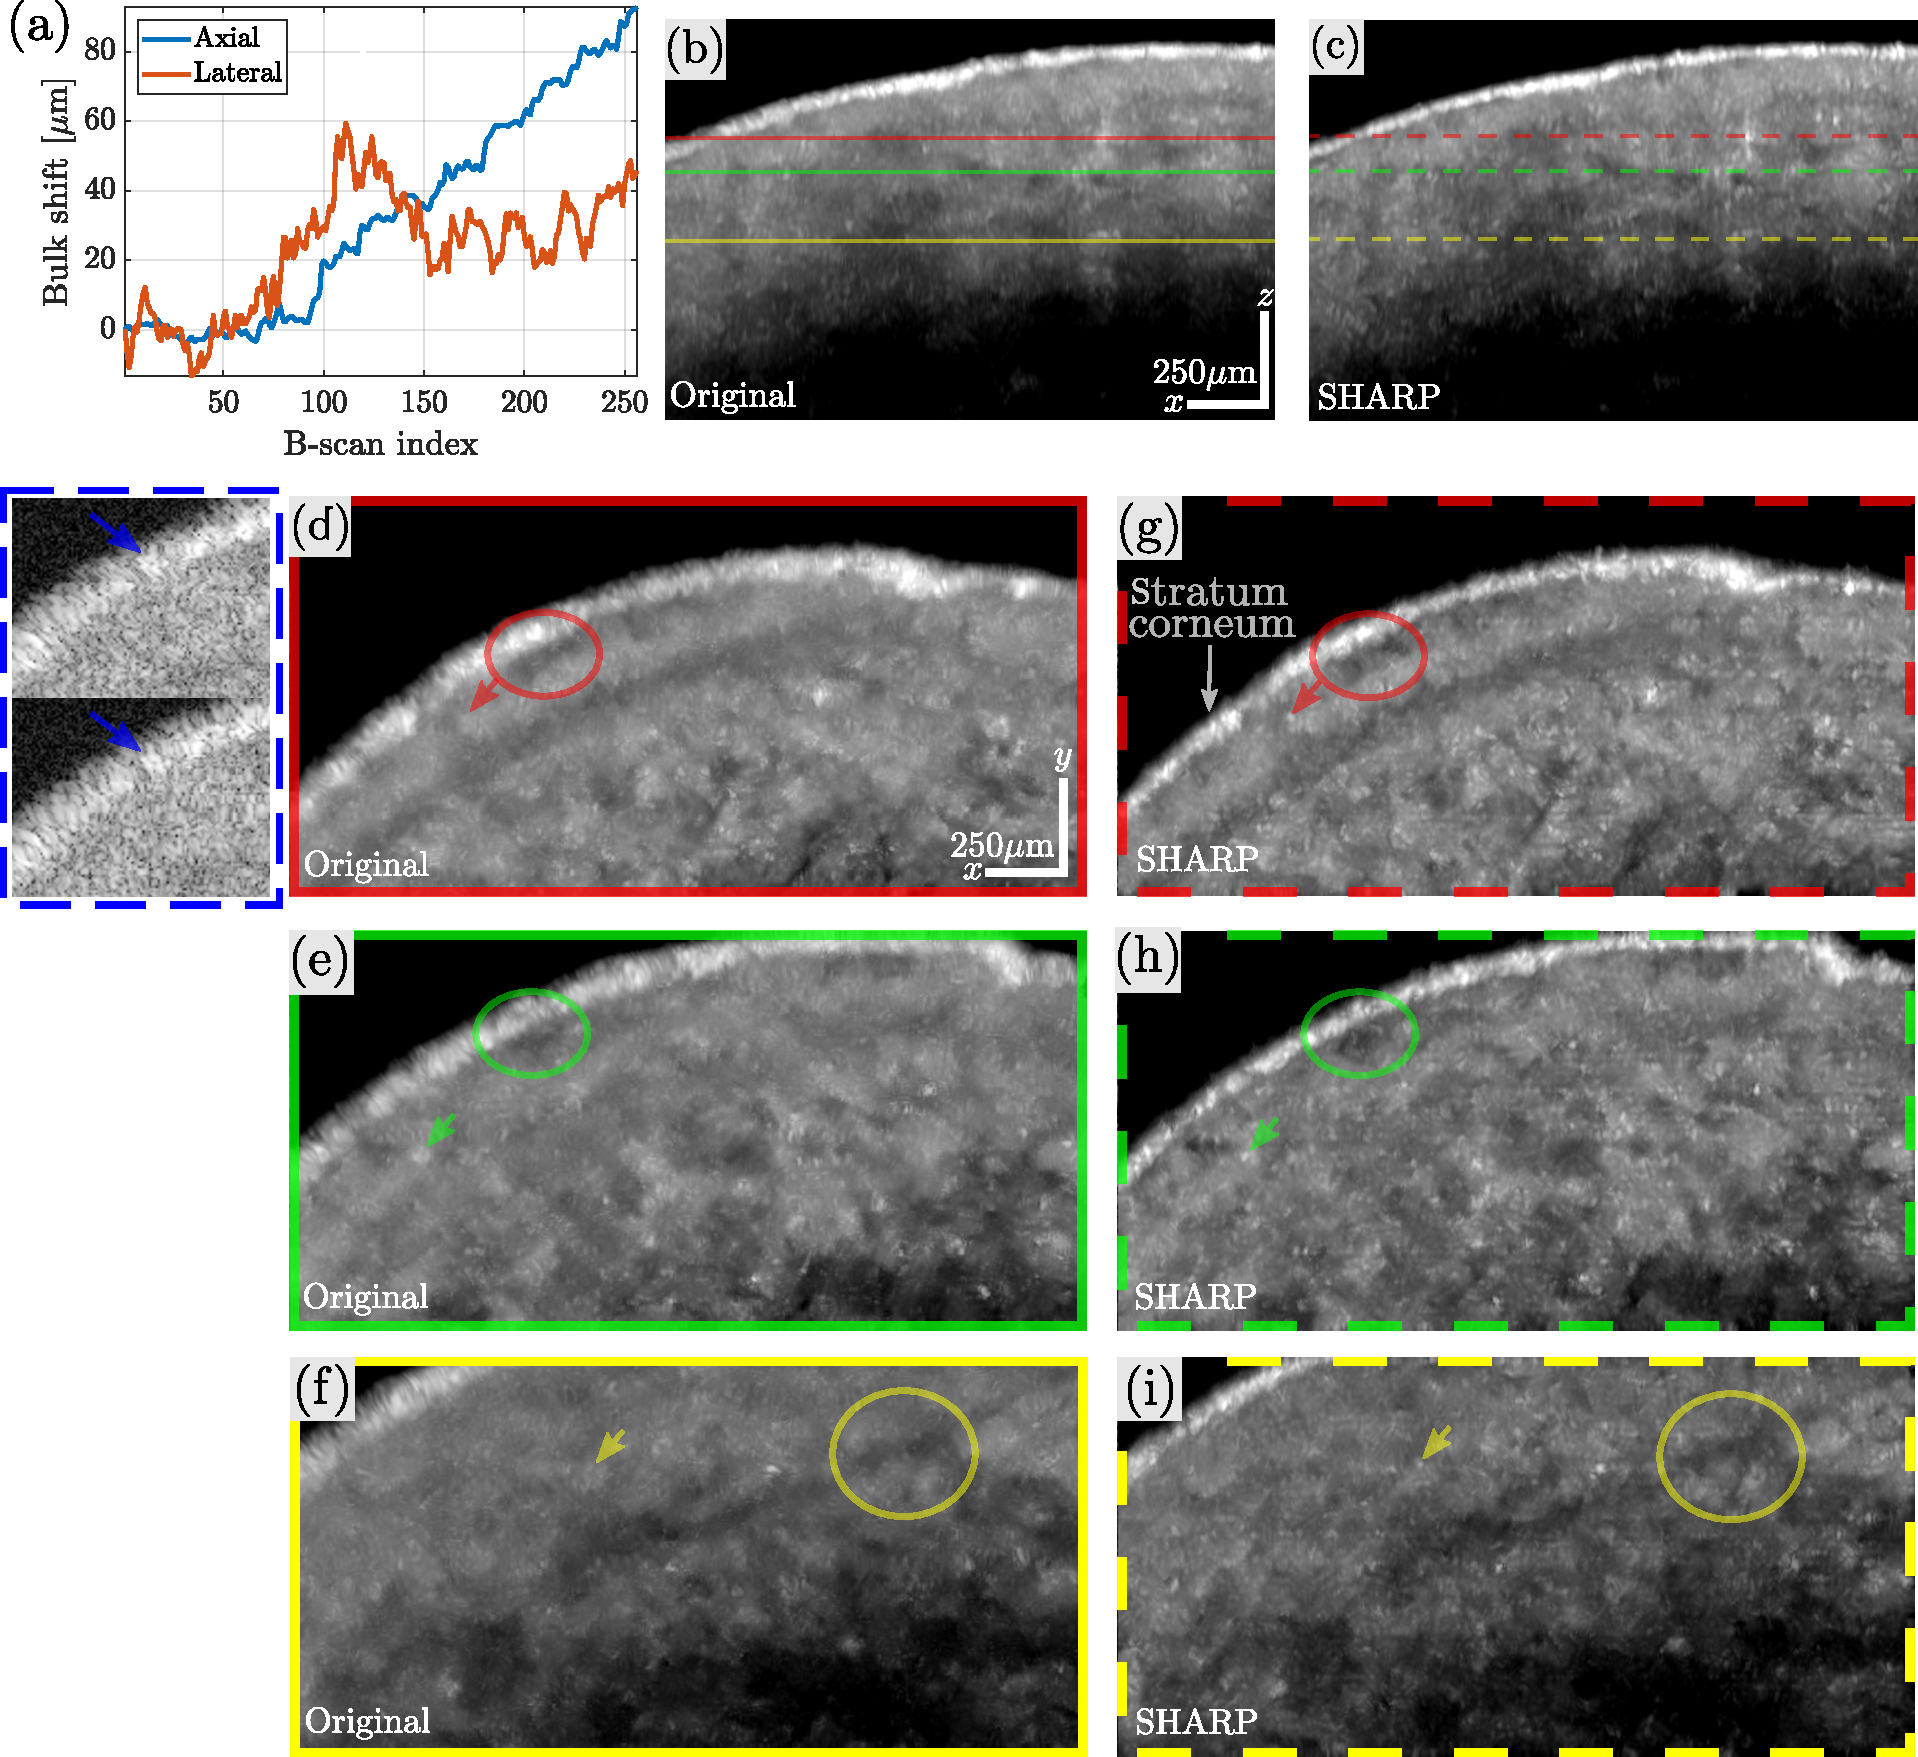
\includegraphics[width=\textwidth]{Figures/Results/SkinImaging.pdf}
	\caption[Application of SHARP in skin imaging \textit{in vivo}]{Application of SHARP in human skin imaging \textit{in vivo}. (a) Axial and lateral shifts determined in motion correction. B-scan views: (b) before and (c) after windows-based SHARP. \textit{En face} views at different depths marked in (b) and (c): (d)-(f) original tomogram and (g)-(i) windows-based SHARP tomogram. Blue inset corresponds to a small \textit{en face} ROI before (top) and after (bottom) motion correction.}
	\label{fig:SkinImaging}
\end{figure}

Figure~\ref{fig:SkinImaging} shows three different \textit{en face} planes of the motion-corrected and SHARP tomograms at depths indicated by the lines on B-scan views in Figs.~\ref{fig:SkinImaging}(b) and (c). Original \textit{en face} views in Figs.\ref{fig:SkinImaging}(e)-(g) present strong blurring, particularly towards the tissue surface, whereas corrected \textit{en faces} in Fig.\ref{fig:SkinImaging}(h)-(j) present sharper features with reduction of smearing that allows to visualize small details throughout the FoV with better contrast. For instance, fine bright structures appear after refocusing such as those marked with arrows and differences in contrast between tissues is observed clearer, like those  enclosed with circles. Most notably, the stratum corneum is brought to focus showing a reduction of the visual thickness. Major limitation of CAC techniques in dermatology is the presence of high multiple scattering that is particularly stronger in skin than in other tissues, frustrating aberration correction for depths deep into the tissue, however, skin imaging is in general shallow given the relatively high light absorption of skin tissue. These successful results demonstrate the ability of SHARP to refocus \textit{in vivo} addressing not only phase noise but complex amplitude shifts as well.

\section{Computational refocusing in polarization-sensitive OCT}

To demonstrate the possibility to preform computational refocusing in PS-OCT, a dataset of the anterior segment of an excised porcine eye was acquired. As seen in the previous experiments, anterior segment imaging is an attractive application that could benefit from computational refocusing due to its surface topography, which posses a long axial extension that precludes the use of medium-NA, and in particular for PS-OCT there is a potential clinical interest in high-resolution polarimetric parameters of tissue in this application~\cite{Li2020_Vectorial}.

The sample was imaged around the limbus with the focal plane located deep into the tissue targeting the trabecular meshwork. The dataset was acquired with the polygon-based SSOCT system and configuration used for the experiment in Section~\ref{sec:CorneaImaging}, but this time activating an integrated electro-optic modulator used to modulate the two illumination orthogonal polarization states between alternating A-lines in the fast scan axis, and using a beam with a $e^{-2}$ diameter of $2w_0=8.5~\mu$m with Rayleigh range $z_R=90~\mu$m in air. The acquired spectra were splitted into 5 spectral windows for the spectral binning processing with an overlap of 66~\% between them. The tomogram contains 1024 B-scans and 1024 A-lines with 1024 depth samples, with a pixel size of 3.3~$\mu$m in lateral axes and $6~\mu$m in the axial axis in air, from which different regions of interest were selected to process. SHARP was applied following the procedure proposed for polarization-sensitive imaging, using only defocus correction since it is the dominant aberration in the experiment, and then the Stokes parameters were spatially-averaged by using a Gaussian kernel with $e^{-2}$ diameter 13$\times$13 $\mu$m$^2$ (4$\times$4 px$^2$) oriented in the lateral axes only.

The analysis was centered on the limbal region, depicted in the B-scan of Figure~\ref{fig:PSOCT_int}(a), where the short vertical yellow line represents the length of the confocal parameter. The focus is visualized approximately in the middle of the yellow box. This configuration is representative of medium-NA imaging of the limbus, where the axial extent of the tissue makes impossible to have the whole ROI in focus. Figs.~\ref{fig:PSOCT_int}(b) and (c) show \textit{en face} intensity views before and after SHARP, respectively, at the depth indicated by the dotted line in Fig.~\ref{fig:PSOCT_int}(a). The intensity after SHARP exhibits a higher contrast and better resolution given the correction of defocus and the effect of the optimum filter.

\begin{figure}[htb!]
	\centering
	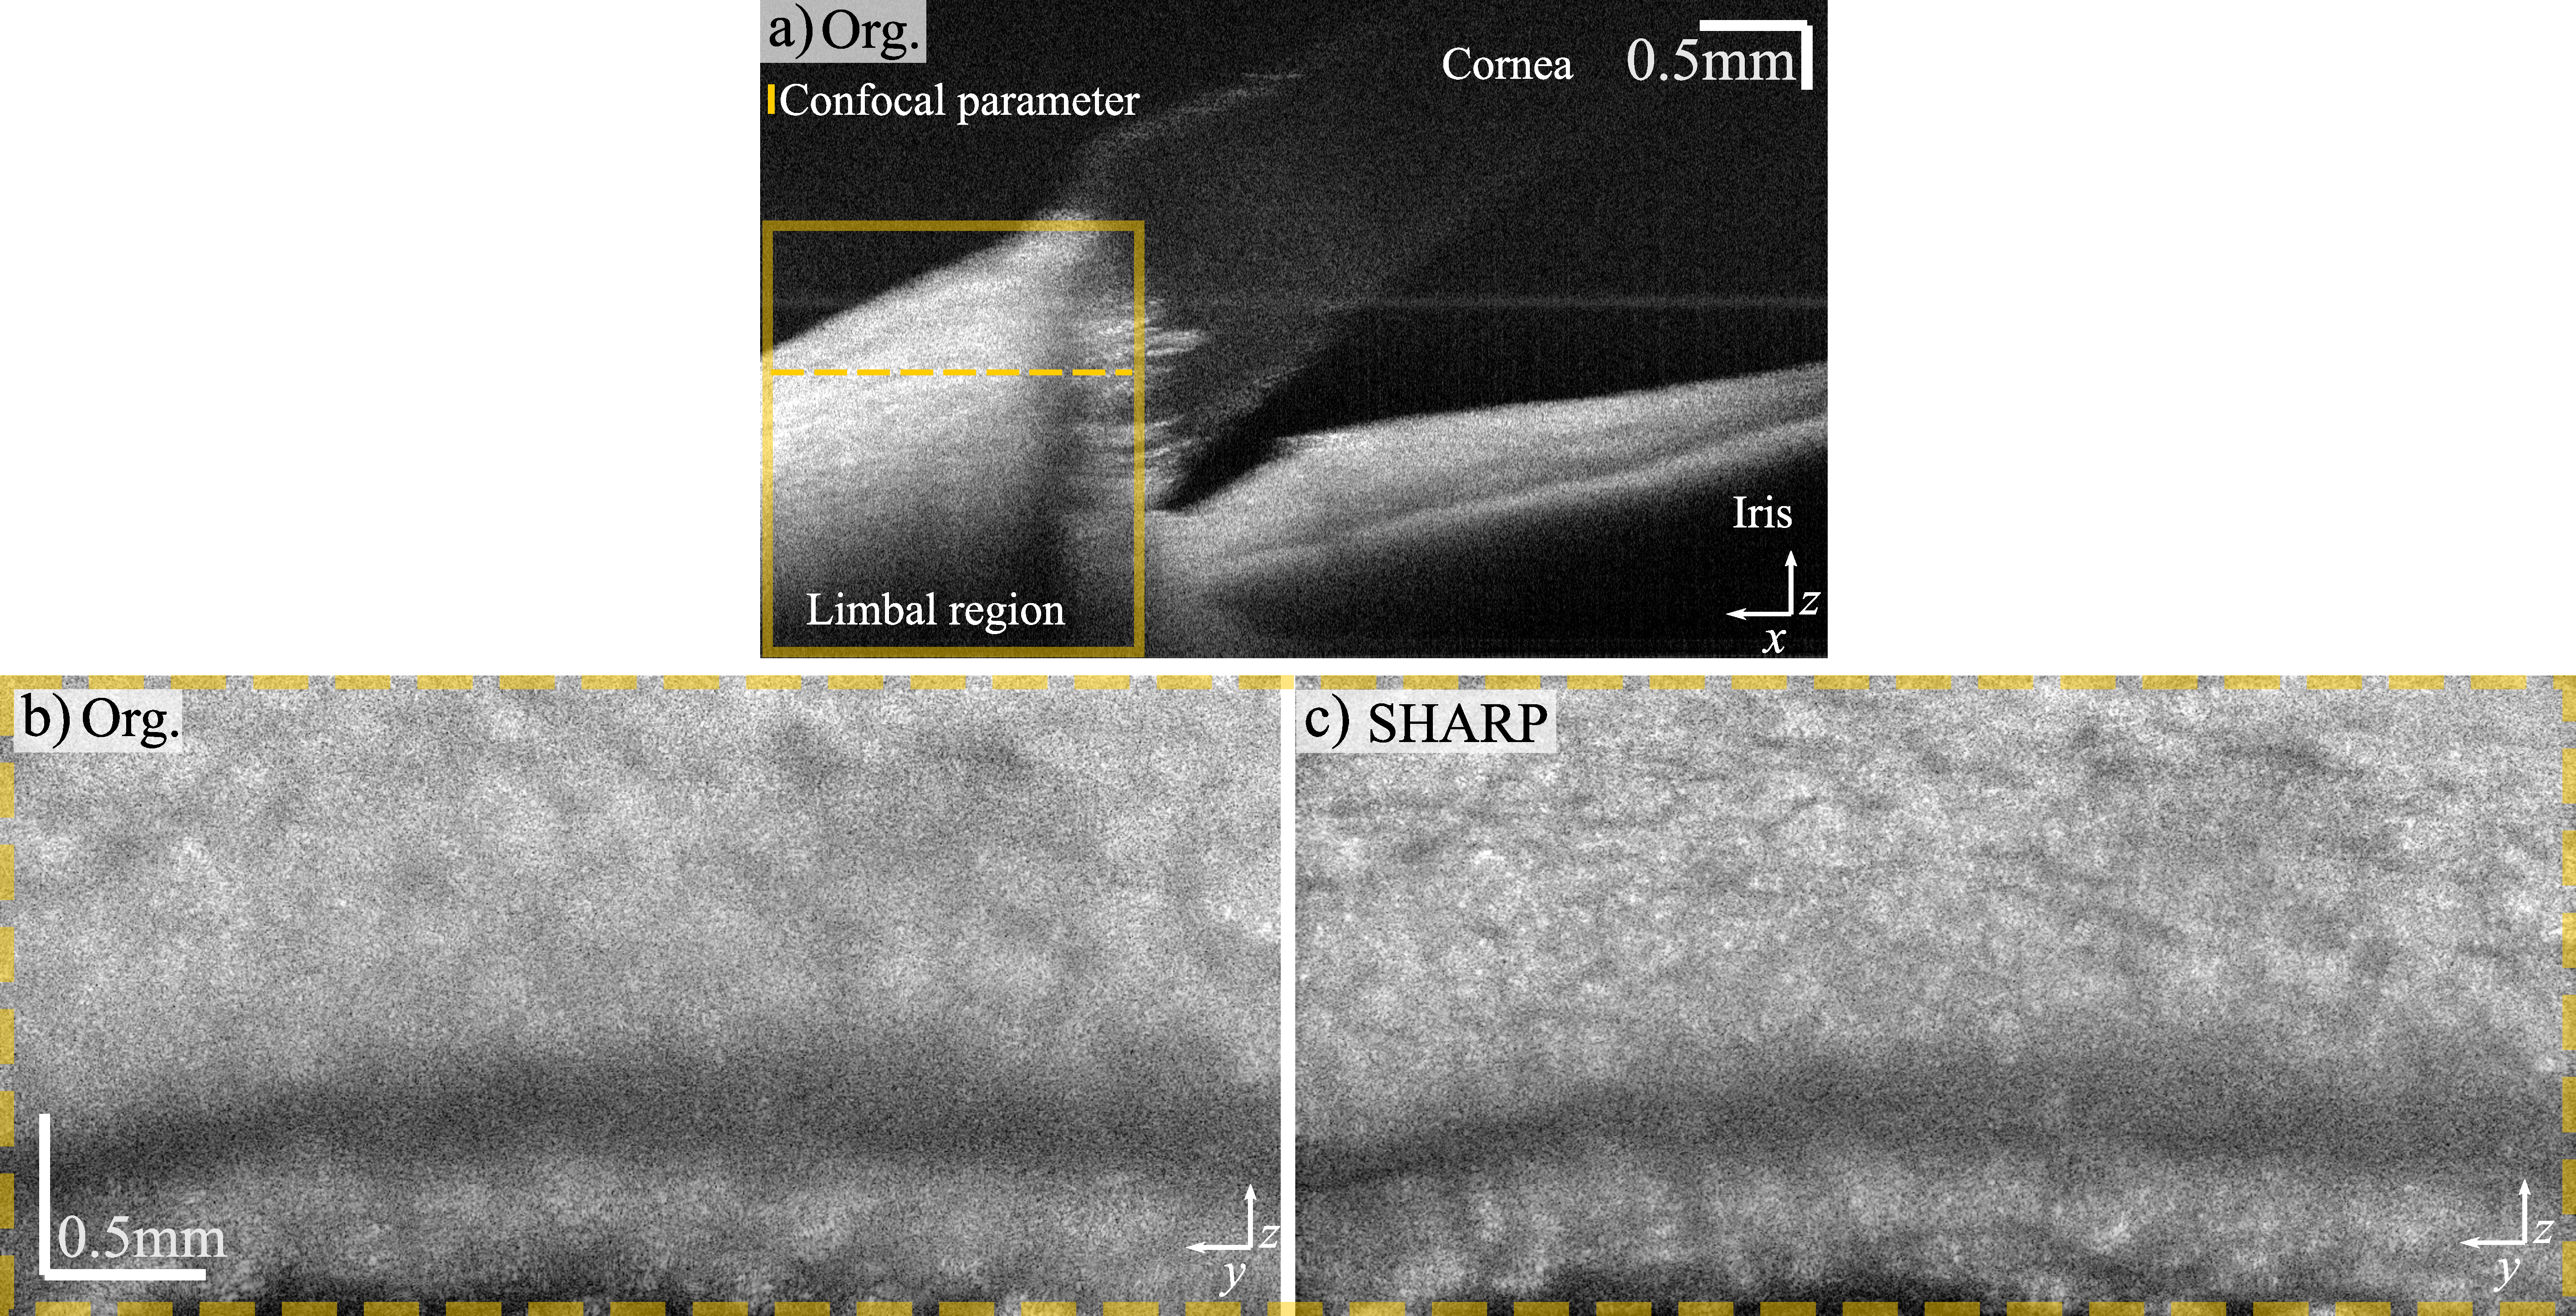
\includegraphics[width=\textwidth]{Figures/Results/PSOCT_Int.pdf}
	\caption[Application of SHARP in polarization-sensitive anterior segment imaging of an excised swine eye.]{Application of SHARP in polarization-sensitive anterior segment imaging of an excised swine eye. (a) B-scan around the limbal region. The limited depth of field is very apparent. The focus is near the center of the solid box. Dotted line indicates location of \textit{en face} views: (b) original (Org.) and (c) after SHARP.}
	\label{fig:PSOCT_int}
\end{figure}

\begin{figure}[b!]
	\centering
	\includegraphics[width=\textwidth]{Figures/Results/PSOCT.pdf}
	\caption[Demonstration of computational refocusing in polarimetric parameters of the anterior segment of an excised swine eye.]{Demonstration of computational refocusing in polarimetric parameters of the anterior segment of an excised swine eye. (a) Intensity B-scan ROI around the solid box in Fig.~\ref{fig:PSOCT_int}. Cross-sectional views of tissue polarimetric parameters, showing original (Org.) and after SHARP side-to-side: (b), (e) DOP (isoluminant colormap) overlaid with intensity (luminance); (c), (f) local retardation for regions with DOP~$>0.65$ over the intensity; (d), (g) optic axis (cyclic isoluminant colormap) overlaid with local retardation (luminance). Axes of each cross-section are indicated in its corresponding panel.}
	\label{fig:PSOCT}
\end{figure}

Figure~\ref{fig:PSOCT} presents cross-sectional views after PS-OCT processing of the original and SHARP tomograms. Fig.~\ref{fig:PSOCT}(a) shows an intensity B-scan view with a yellow line marking the location of the cross-sectional views on Figs.~\ref{fig:PSOCT}(b)-(d), and a red line marking the location for the \textit{en face} views on Figs.~\ref{fig:PSOCT}(e)-(g); all insets show different tissue polarimetric parameters of the original data and the SHARP data side-to-side. The degree of polarization (DOP) is overlaid with the intensity in Figs.~\ref{fig:PSOCT}(b) and (e), local retardation is shown in Figs.~\ref{fig:PSOCT}(c) and (f) using a DOP threshold to display the intensity where DOP is $<0.65$, and the optic axis is overlaid with the local retardation in Figs.~\ref{fig:PSOCT}(d) and (g). Structures in the uncorrected images appear highly affected by defocus, spatial averaging and spectral binning. Polarimetric parameters calculated after SHARP do not exhibit any corruption in their information, furthermore successful refocusing is indicated by the clear improvement in spatial resolution in the polarimetric parameters, indicating that PS-OCT processing is indeed compatible with computational refocusing. 

Correcting for defocus reveals structures that appear blurred in the original tomograms, exhibiting better contrast and sharpness associated with the improvement of lateral resolution. This is noticeable in all polarimetric images, especially in the \textit{en face} views given that refocusing operates on both lateral axes. In particular, ridges-like structures can be visualized in the DOP images with SHARP, that may be associated with the Palisades of Vogt which are functionally important structures containing stem cells, associated with the regeneration of the corneal tissue after damage~\cite{Bizheva2017_Invivo}. 

There are two main limitations to the use of SHARP in PS-OCT. First, axial resolution of retardance and optic axis depend on the magnitude of spectral binning and the step size for local PS processing~\cite{Villiger2013_Spectral}. Thus, cross-sectional views [like Figs.~\ref{fig:PSOCT}(b)-(d)] show a less remarkable improvement than \textit{en face} views in which defocus is corrected in both axes [like Figs.~\ref{fig:PSOCT}(e)-(g)]. Axial resolution loss that occurs in spectral binning Stokes processing can be avoided using Mueller processing~\cite{Li2018_Robust} but in this case phase stability becomes relevant because input orthogonal polarization states have to be phase-stable between them which currently is not achieved with SHARP. It could be possible to develop an strategy to leverage from the 1D phase stability like in SHARP but oriented to the tomograms from the two input polarization states to perform a full correction of the wavelength-dependent noise introduce by the system while maintaining the full axial resolution by using Mueller processing~\cite{Li2018_Robust}. Although this will limit spatial averaging to the axial and only one lateral dimensions, this could have attractive implications for the extraction of diattenuation information from tissue imaged with inter-A-line modulation PS-OCT systems, such as those used in intravascular OCT.

Second, the improvement in lateral resolution after SHARP is partially neutralized by the spatial averaging required for PS-OCT processing. For this reason, advanced resolution-preserving despeckling is demanded in order to take full advantage of computational refocusing in PS-OCT. An extension of TNode to despeckle Stokes parameters is on current development, called polarization-sensitive-TNode (PS-TNode) and its combination with SHARP promises to be a powerful tool to improve and preserve resolution in PS-OCT imaging.
\newpage
\phantomsection
\chapter{Conclusions and future works}\label{chap:conclusions}



% Referencias
\addcontentsline{toc}{chapter}{REFERENCES}
%\section*{Referencias}
\bibliographystyle{unsrt}
\bibliography{bibsource}

\end{document}